\documentclass{problemset}

%%%
% import all needed packages and macros
%%%
%%
%% All packages and macros needed for the problemsets
%%

\usepackage{amsmath}

\usepackage{lipsum}
%\usepackage{showframe}
%\usepackage{layout}


\usepackage[charter,cal=cmcal]{mathdesign} %different font
%\usepackage{avant}

\usepackage{microtype}
\usepackage{mathtools}
\usepackage{etoolbox}
%\usepackage{amsfonts}
%\usepackage{amssymb}
\usepackage{graphicx}
\usepackage[inline]{enumitem}
\usepackage{xparse}
\usepackage{ifthen}
\usepackage{graphicx}
\usepackage{caption}
\usepackage{subcaption}
\usepackage{color}
\usepackage{tikz}
	\usetikzlibrary{fit}
	\usetikzlibrary{fadings}
	\usetikzlibrary{calc}
	\tikzset{>=latex}
	\usetikzlibrary{cd}
\usepackage{fancyhdr}
\usepackage{calc}
\usepackage{wrapfig}
\usepackage{marginnote}
\usepackage{mparhack}
\usepackage{marginfix}
\usepackage[hidelinks]{hyperref}
\usepackage{fnpct} % fancy footnote spacing
\usepackage{bm}
\usepackage{systeme}
\usepackage{datatool}% http://ctan.org/pkg/datatool for sorted lists



\usepackage{pgfplots}
\pgfplotsset{compat=newest}
%%%
% Useful Linear Algebra macros
%%%
\newcommand{\declarecommand}[1]{\providecommand{#1}{}\renewcommand{#1}}
\declarecommand{\R}{\mathbb{R}}  % we don't care if it's already defined.  We really want *this* command!
\declarecommand{\Z}{\mathbb{Z}}
\declarecommand{\Q}{\mathbb{Q}}
\declarecommand{\N}{\mathbb{N}}
\declarecommand{\C}{\mathbb{C}}
\declarecommand{\d}{\mathrm{d}}
\declarecommand{\dd}{\mathbbm{d}} % exterior derivative
\DeclareMathOperator{\Span}{span}
\DeclareMathOperator{\Img}{img}
\DeclareMathOperator{\Id}{id}
\DeclareMathOperator{\Ident}{\Id}
\DeclareMathOperator{\Vol}{Vol}
\DeclareMathOperator{\VolChange}{Vol\hspace{1.5pt}Change}
\DeclareMathOperator{\Range}{range}
\DeclareMathOperator{\Rref}{rref}
\DeclareMathOperator{\Rank}{rank}
\DeclareMathOperator{\Comp}{\Vcomp}
\DeclareMathOperator{\Vcomp}{v\hspace{1pt}comp}
\DeclareMathOperator{\Null}{null}
\DeclareMathOperator{\Nullity}{nullity}
\DeclareMathOperator{\Char}{char}
\DeclareMathOperator{\Proj}{proj}
\DeclareMathOperator{\Flux}{Flux}
\DeclareMathOperator{\Circ}{Circ}
\DeclareMathOperator{\chr}{char}
\DeclareMathOperator{\Dim}{dim}
\DeclareMathOperator{\Perp}{perp}
\DeclareMathOperator{\Ker}{kernel}
\DeclareMathOperator{\Row}{row}
\DeclareMathOperator{\Col}{col}
\DeclareMathOperator{\Rep}{Rep}
\newcommand{\BasisChange}[2]{[#2\!\leftarrow\!#1]}
\newcommand{\proj}{\Proj}
\newcommand{\rref}{\Rref}
\newcommand{\xhat}{{\vec e_1}}
\newcommand{\yhat}{{\vec e_2}}
\newcommand{\zhat}{{\vec e_3}}
\newcommand{\sbasis}[1]{\vec { e}_{#1}}
\newcommand{\mat}[1]{\begin{bmatrix*}[r]#1\end{bmatrix*}}
\newcommand{\matc}[1]{\begin{bmatrix}#1\end{bmatrix}}
\newcommand{\formarg}[2]{\big(#1;\, #2\big)}
\DeclarePairedDelimiter\abs{\lvert}{\rvert}
\DeclarePairedDelimiter\Abs{\lvert}{\rvert}
\DeclarePairedDelimiter\norm{\lVert}{\rVert}
\newcommand{\Norm}[1]{\norm{#1}}
% just to make sure it exists
\providecommand\given{}
% can be useful to refer to this outside \Set
\newcommand\SetSymbol[1][]{%
	\nonscript\::%
	\allowbreak
	\nonscript\:
	\mathopen{}}
\DeclarePairedDelimiterX\Set[1]\{\}{%
	\renewcommand\given{\SetSymbol[\delimsize]}
	#1
}


%%%
% Set up the footers to have the correct copyright notices
%%%

\fancypagestyle{siefken}{%
	\rfoot{\footnotesize\it \copyright\,Jason Siefken, 2015--2019 \ \makebox(30,5){\includegraphics[height=1.2em]{by-sa.pdf}}}
	\lfoot{}
	\renewcommand{\headrulewidth}{0pt}
}
\fancypagestyle{iola}{%
	\rfoot{\footnotesize\it \copyright\,IOLA Team \url{iola.math.vt.edu} \ \makebox(30,5){\includegraphics[height=2.2em]{images/iolalogo.png}}}
	\lfoot{}
	\renewcommand{\headrulewidth}{0pt}
}

\DeclareDocumentEnvironment{iola}{o}{%
	\newpage
	\pagestyle{iola}
}{%
	\newpage
}


%%
% Allow hiding of environments
%%
\usepackage{environ}% http://ctan.org/pkg/environ
\makeatletter
\newcommand{\voidenvironment}[1]{%
  \expandafter\providecommand\csname env@#1@save@env\endcsname{}%
  \expandafter\providecommand\csname env@#1@process\endcsname{}%
  \@ifundefined{#1}{}{\RenewEnviron{#1}{}}%
}
\makeatother
% allow pagebreaks that only display in `standard` mode
\newcommand{\displayonlynewpage}{\begin{displayonly}\newpage\end{displayonly}}
% allow pagebreaks that only display in `book` mode
\newcommand{\bookonlynewpage}{\begin{bookonly}\newpage\end{bookonly}}

%
% Set up the three render modes: standard, instructor, and solutions.
% These render with varying amounts of extra data (like solutions and notes)
%
\newtoggle{instructor}
\newtoggle{standard}
\newtoggle{solutions}
\newtoggle{book}
\newcommand{\setinstructor}{
	\toggletrue{instructor}
	\togglefalse{standard}
	\togglefalse{solutions}
	\togglefalse{book}
}
\newcommand{\setstandard}{
	\togglefalse{instructor}
	\toggletrue{standard}
	\togglefalse{solutions}
	\togglefalse{book}
}
\newcommand{\setsolutions}{
	\togglefalse{instructor}
	\togglefalse{standard}
	\toggletrue{solutions}
	\togglefalse{book}
}
\newcommand{\setbook}{
	\togglefalse{instructor}
	\togglefalse{standard}
	\togglefalse{solutions}
	\toggletrue{book}
	\setbookgeometry
}

%
% Infer the document level from the \jobname
%
\usepackage{xstring}
\IfSubStr{\jobname}{\detokenize{book}}{\setbook}{
	\IfSubStr{\jobname}{\detokenize{solutions}}{\setsolutions}{
		\IfSubStr{\jobname}{\detokenize{instructor}}{\setinstructor}{
			\setstandard
		}
	}
}

%
% Hide the non-problem environments
%
\newcommand{\coversubtitle}{} % we override the subtitle in each mode, so make sure the command exists to override.
\iftoggle{instructor}{
	\voidenvironment{module}
	\voidenvironment{bookonly}
	\voidenvironment{displayonly}
	\renewcommand{\coversubtitle}{Instructor Guide}
}{}
\iftoggle{solutions}{
	\voidenvironment{module}
	\voidenvironment{bookonly}
	\voidenvironment{displayonly}
	\voidenvironment{lesson}
	\voidenvironment{notes}
	\renewcommand{\coversubtitle}{Solutions}
}{}
\iftoggle{standard}{
	\voidenvironment{module}
	\voidenvironment{bookonly}
	\voidenvironment{solution}
	\voidenvironment{annotation}
	\voidenvironment{lesson}
	\renewcommand{\coversubtitle}{MAT223 Notes}
}{}
\iftoggle{book}{
	\voidenvironment{displayonly}
	\voidenvironment{solution}
	\voidenvironment{annotation}
	\voidenvironment{lesson}
	\renewcommand{\coversubtitle}{MAT223 Workbook}
}{}
%\voidenvironment{solution}
%\voidenvironment{annotation}
%\voidenvironment{lesson}
%%\voidenvironment{notes}
%%\voidenvironment{displayonly}




\begin{document}
%%
%% Import definitions from definition.tex; all definitions can be restated multiple times
%%

%%
%% Start Definitions (each of these we can reuse)
%%
\begin{SaveDefinition}[
		key=SubsetSuperset,
		title={Subset \& Superset}
	]
	The set $B$ is a \emph{subset}\index[definitions]{Subset} of the set $A$, written $B\subseteq A$\index[symbols]{$\subseteq$}, if for all
	$b\in B$ we also have $b\in A$.  In this case, $A$ is called a \emph{superset}\index[definitions]{Superset}
	of $B$.\footnote{
		Some mathematicians use the symbol $\subset$ instead of $\subseteq$.}
\end{SaveDefinition}
\begin{SaveDefinition}[
		key=SetEquality,
		title={Set Equality}
	]
	The sets $A$ and $B$ are \emph{equal}\index{Set!equality}\index[definitions]{Set!equality}, written $A=B$, if $A\subseteq B$ and $B\subseteq A$.
\end{SaveDefinition}
\begin{SaveDefinition}[
		key=SetSubtraction,
		title={Set Subtraction}
	]
	For sets $A$ and $B$, the \emph{set-wise difference}\index[definitions]{Set!subtraction}\index{Set!subtraction} between $A$ and $B$,
	written $A\backslash B$, is the set
	\[
		A\backslash B = \Set{x\given x\in A\text{ and }x\notin B}.
	\]
\end{SaveDefinition}
\begin{SaveDefinition}[
		key=UnionsIntersections,
		title={Unions \& Intersections}
	]
	Let $X$ and $Y$ be sets. The \emph{union}\index[definitions]{Set!union}\index{Set!union}\index[symbols]{$\cup$} of $X$ and $Y$ and the 
	\emph{intersection}\index[definitions]{Set!intersection}\index{Set!intersection}\index[symbols]{$\cap$} of $X$
	and $Y$ are defined as follows.

	\smallskip

	\hfill\begin{minipage}{\dimexpr\textwidth-3cm}
	\begin{itemize}
		\item[(union)] $X\cup Y = \Set{ a \given a\in X\text{ or }a\in Y}$.
		\item[(intersection)] $X\cap Y = \Set{ a \given a\in X\text{ and }a\in Y}$.
	\end{itemize}
	\end{minipage}
\end{SaveDefinition}

\begin{SaveDefinition}[key=Set, title={Set}]
	A \emph{set}\index[definitions]{Set} is a (possibly infinite) collection of items and is notated
	with curly braces (for example, $\{1,2,3\}$ is the set containing the
	numbers 1, 2, and 3). We call the items in a set
	\emph{elements}.

	If $X$ is a set and $a$ is an element of $X$, we may write $a\in X$,
	which is read ``$a$ is an element of $X$.''

	If $X$ is a set, a
	\emph{subset} $Y$ of $X$ (written $Y\subseteq X$) is a set such that
	every element of $Y$ is an element of $X$. Two sets are called
	\emph{equal} if they are subsets of each other (i.e., $X=Y$ if $X\subseteq
	Y$ and $Y\subseteq X$).

	We can define a subset using
	\emph{set-builder notation}. That is, if $X$ is a set, we can define the
	subset
	\[
		Y= \Set*{a\in X \given \text{some rule involving }a},
	\]
	 which is read ``$Y$ is the set of $a$ in $X$ {\bf such that} some rule
	involving $a$ is true.'' If $X$ is intuitive, we may omit it and simply write
	$Y=\{a:\text{some rule involving }a\}$. You may equivalently use ``$|$''
	instead of ``$:$'', writing $Y=\{a\,|\,\text{some rule involving }a\}$.
\end{SaveDefinition}

\begin{SaveDefinition}[key=ZeroVector, title={Zero Vector}]
		The \emph{zero vector}\index{Zero vector ($\vec 0$)}\index[definitions]{Zero vector ($\vec 0$)}, notated as $\vec 0$\index[symbols]{$\vec 0$},
		is the vector with no magnitude.
\end{SaveDefinition}

\begin{SaveDefinition}[key=LinearCombination, title={Linear Combination}]
	A \emph{linear combination}\index{Linear combination}\index[definitions]{Linear combination} of the vectors
	$\vec v_{1},\vec v_{2},\ldots,\vec v_{n}$ is a vector
	\[
		\vec w = \alpha_{1}\vec v_{1}+\alpha_{2}\vec v_{2}+\cdots+\alpha_{n}\vec
		v_{n}.
	\]
	 The scalars $\alpha_{1},\alpha_{2},\ldots,\alpha_{n}$ are called the
	\emph{coefficients}\index{Linear combination!coefficient of}\index[definitions]{Linear combination!coefficient of} of the linear combination.
\end{SaveDefinition}

\begin{SaveDefinition}[
	key=NonnegativeConvexLinearCombinations,
	title={Non-negative \& Convex Linear Combinations}]

	Let
	$\vec w=\alpha_{1}\vec v_{1}+\alpha_{2}\vec v_{2}+\cdots+\alpha_{n}\vec
	v_{n}.$
	The vector $\vec w$ is called a 
	\emph{non-negative}\index{Linear combination!non-negative}\index[definitions]{Linear combination!non-negative} linear combination of
	$\vec v_{1},\vec v_{2},\ldots,\vec v_{n}$ if
	\[\alpha_{1},\alpha_{2},\ldots,\alpha_{n}\geq 0.\]

	The vector $\vec w$ is called a 
	\emph{convex}\index{Linear combination!convex}\index[definitions]{Linear combination!convex} linear combination of
	$\vec v_{1},\vec v_{2},\ldots,\vec v_{n}$
	if \[\alpha_{1},\alpha_{2},\ldots,\alpha_{n}\geq 0\qquad\text{and}\qquad
	\alpha_{1}+\alpha_{2}+\cdots+\alpha_{n}=1.\]
\end{SaveDefinition}

\begin{SaveDefinition}[key=VectorFormofaLine, title={Vector Form of a Line}]
	Let $\ell$ be a line and let $\vec d$ and $\vec p$ be vectors. If $\ell=\Set{\vec
	x\given \vec x= t\vec d+\vec p\text{ for some } t\in\R }$, we say the vector equation

	\[
		\vec x=t\vec d+\vec p
	\]
	 is $\ell$ expressed in
	\emph{vector form}\index{Line!vector form of}\index[definitions]{Line!vector form of}. The vector $\vec d$ is called a
	\emph{direction vector}\index{Line!direction vector for}\index[definitions]{Line!direction vector for} for $\ell$.
\end{SaveDefinition}

\begin{SaveDefinition}[key=VectorFormofaPlane, title={Vector Form of a Plane}]
	A plane $\mathcal P$ is written in
	\emph{vector form}\index{Plane!vector form of}\index[definitions]{Plane!vector form of} if it is expressed as
	\[
		\vec x=t\vec d_{1} +s\vec d_{2}+\vec p
	\]
	 for some vectors $\vec d_{1}$ and $\vec d_{2}$ and point $\vec p$. That
	is,
	$\mathcal P = \{\vec x: \vec x= t\vec d_{1}+s\vec d_{2} +\vec p\text{ for
	some }t,s\in\R \}$. The vectors $\vec d_{1}$ and $\vec d_{2}$ are called
	\emph{direction vectors}\index{Plane!direction vector for}\index[definitions]{Plane!direction vector for} for $\mathcal P$.
\end{SaveDefinition}

\begin{SaveDefinition}[key=Span, title={Span}]
	The
	\emph{span}\index{Span}\index[definitions]{Span} of a set of vectors $V$ is the set of all linear
	combinations of vectors in $V$. That is,
	\[
		\Span V = \Set{\vec v \given \vec v=\alpha_1\vec v_1+\alpha_2\vec
		v_2 + \cdots +\alpha_n\vec v_n\text{ for some }\vec v_1,\vec v_2,\ldots,\vec
		v_n\in V \text{ and scalars }\alpha_1,\alpha_2,\ldots,\alpha_n}.
	\]
	\index[symbols]{$\Span V$}

	Additionally, we define $\Span\Set{} = \Set{\vec 0}$.
\end{SaveDefinition}

\begin{SaveDefinition}[key=SetAddition, title={Set Addition}]
	If $A$ and $B$ are sets of vectors, then the
	\emph{set sum}\index{Set sum}\index[definitions]{Set sum} of $A$ and $B$, denoted $A+B$, is
	\[
		A+B=\Set{\vec x \given \vec x=\vec a+\vec b\text{ for some }\vec
		a\in A\text{ and } \vec b\in B}.
	\]

\end{SaveDefinition}

\begin{SaveDefinition}[
	key=LinearlyDependentIndependentGeometric,
	title={Linearly Dependent \& Independent (Geometric)}]

	We say the vectors $\vec v_{1},\vec v_{2},\ldots,\vec v_{n}$ are
	\emph{linearly dependent}\index{Linearly dependent} if for at least one $i$,
	\[
		\vec v_{i}\in\Span\Set{\vec v_1,\vec v_2,\ldots,\vec v_{i-1}, \vec
		v_{i+1},\ldots,\vec v_n}.
	\]
	 Otherwise, they are called
	\emph{linearly independent}\index{Linearly independent}\index[definitions]{Linear dependence/independence!geometric definition}.
\end{SaveDefinition}

\begin{SaveDefinition}[
	key=TrivialLinearCombination,
	title={Trivial Linear Combination}]

	The linear combination $\alpha_1\vec v_1+\cdots+\alpha_n\vec v_n$ is called
	\emph{trivial}\index{Linear combination!trivial}\index[definitions]{Linear combination!trivial}
	if $\alpha_1=\cdots=\alpha_n=0$. If at least one $\alpha_i\neq 0$,
	the linear combination is called \emph{non-trivial}.
\end{SaveDefinition}

\begin{SaveDefinition}[
	key=LinearlyDependentIndependentAlgebraic,
	title={Linearly Dependent \& Independent (Algebraic)}]

	The vectors $\vec v_{1},\vec v_{2},\ldots,\vec v_{n}$ are
	\emph{linearly dependent} if there is a non-trivial linear combination
	of $\vec v_{1},\ldots,\vec v_{n}$ that equals the zero vector. Otherwise they
	are linearly independent\index[definitions]{Linear dependence/independence!algebraic definition}.
\end{SaveDefinition}

\begin{SaveDefinition}[
	key=HomogeneousSystem,
	title={Homogeneous System}]

	A system of linear equations or a vector equation in the variables $\alpha_1$, \ldots, 
	$\alpha_n$ is called
	\emph{homogeneous}\index{System of linear equations!homogeneous}\index[definitions]{Homogeneous system} if it takes the form
	\[
		\alpha_1\vec v_1+\alpha_2\vec v_2+\cdots +\alpha_n\vec v_n=\vec 0,
	\]
	where the right side of the equation is $\vec 0$.
\end{SaveDefinition}


\begin{SaveDefinition}[key=Norm, title={Norm}]
	The
	\emph{norm} of a vector $\vec v=\matc{v_1\\\vdots\\v_n}$ is the length/magnitude
	of $\vec v$. It is written $\|\vec v\|$ and can be computed from the Pythagorean
	formula
	\[
		\|\vec v\|=\sqrt{v_1^2+\cdots +v_n^2}.
	\]

\end{SaveDefinition}

\begin{SaveDefinition}[key=DotProduct, title={Dot Product}]
	If $\vec a=\matc{a_1\\a_2\\ \vdots\\a_n}$ and
	$\vec b=\matc{b_1\\b_2\\ \vdots\\b_n}$ are two vectors in $n$-dimensional
	space, then the
	\emph{dot product} of $\vec a$ an $\vec b$ is
	\[
		\vec a\cdot\vec b = a_{1}b_{1}+a_{2}b_{2}+\cdots+a_{n}b_{n}.
	\]
	 Equivalently, the dot product is defined by the geometric formula
	\[
		\vec a\cdot \vec b = \|\vec a\|\|\vec b\|\cos \theta
	\]
	 where $\theta$ is the angle between $\vec a$ and $\vec b$.
\end{SaveDefinition}

\begin{SaveDefinition}[key=Direction, title={Direction}]
	The vector $\vec u$ points in the \emph{direction}\index{Direction}\index{Vector!positive direction of} of
	the vector $\vec v$ if $k\vec u=\vec v$ for some scalar $k$.
	The vector $\vec u$ points in the \emph{positive direction} of
	$\vec v$ if $k\vec u=\vec v$ for some positive scalar $k$.
\end{SaveDefinition}

\begin{SaveDefinition}[key=Distance, title={Distance}]
	The
	\emph{distance} between two vectors $\vec u$ and $\vec v$ is
	$\|\vec u-\vec v\|$.
\end{SaveDefinition}

\begin{SaveDefinition}[key=UnitVector, title={Unit Vector}]
	A vector $\vec v$ is called a
	\emph{unit vector} if $\|\vec v\|=1$.
\end{SaveDefinition}

\begin{SaveDefinition}[key=Orthogonal, title={Orthogonal}]
	Two vectors $\vec u$ and $\vec v$ are
	\emph{orthogonal}\index{Orthogonal}\index[definitions]{Orthogonal} to each other if $\vec u\cdot \vec v=0$. The word orthogonal
	is synonymous with the word perpendicular.
\end{SaveDefinition}

\begin{SaveDefinition}[key=NormalVector, title={Normal Vector}]
	A
	\emph{normal vector}\index[definitions]{Line!normal vector}\index{Plane!normal vector}\index{Line!normal vector}\index{Plane!normal vector} to a line (or plane or hyperplane) is a non-zero
	vector that is orthogonal to all direction vectors for the line (or plane
	or hyperplane).
\end{SaveDefinition}

\begin{SaveDefinition}[key=NormalFormofaLine, title={Normal Form of a Line}]

	A line $\ell\subseteq \R^2$ is expressed in \emph{normal form}\index[definitions]{Line!normal form}\index{Line!normal form} if there exist
	vectors $\vec n\neq \vec 0$ and $\vec p$ so that $\ell$ is the solution set to the equation
	\[
		\vec n\cdot (\vec x-\vec p)=0.
	\]
	The equation $\vec n\cdot (\vec x-\vec p)=0$ is called the \emph{normal form of $\ell$}.
\end{SaveDefinition}

\begin{SaveDefinition}[key=Hyperplane, title={Hyperplane}]
	The set $X\subseteq \R^n$ is called a \emph{hyperplane}\index{Hyperplane}\index[definitions]{Hyperplane} if there
	exists $\vec n\neq \vec 0$ and $\vec p$ so that $X$ is the set of solutions
	to the equation
	\[
		\vec n\cdot (\vec x-\vec p)=0.
	\]
\end{SaveDefinition}


\begin{SaveDefinition}[key=Projection, title={Projection}]
	Let $X$ be a set. The
	\emph{projection} of the vector $\vec v$ onto $X$, written $\Proj_{X}\vec
	v$, is the closest point in $X$ to $\vec v$.\index[definitions]{Projection}\index{Projection}\index[symbols]{$\Proj_{X}\vec v$}
\end{SaveDefinition}

\begin{SaveDefinition}[key=Component, title={Vector Components}]
	Let $\vec u$ and $\vec v\neq \vec 0$ be vectors. The
	\emph{vector component of $\vec u$ in the $\vec v$ direction}, written $\Comp_{\vec
	v}\vec u$, is the vector in the direction of $\vec v$ so that
	$\vec u-\Comp_{\vec v}\vec u$ is orthogonal to $\vec v$.\index{Vector component}\index[definitions]{Vector component}\index[symbols]{$\Vcomp_{\vec v}\vec u$}
	\begin{center}
		\usetikzlibrary{patterns, decorations.pathreplacing}
		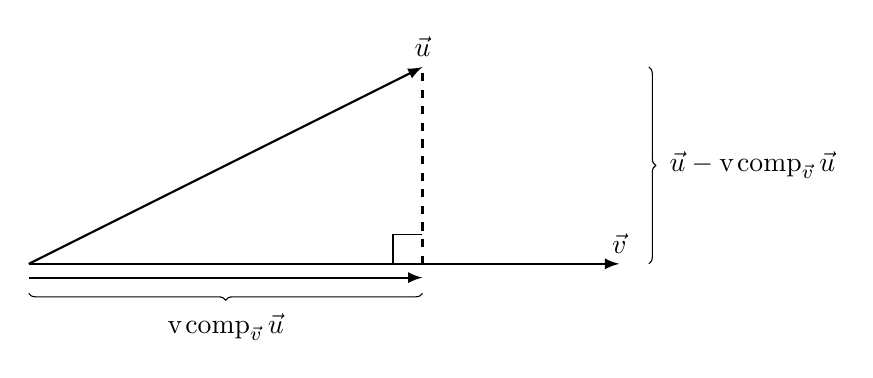
\begin{tikzpicture}[>=latex, scale=2.5]
			\draw[->,thick,black] (0,0) -- (2,1) node [above]
				{$\vec u$};

			\draw[->,thick,black] (0,0) -- (3,0) node [above]
				{$\vec v$};

			\draw[->,thick,black,yshift=-.07cm] (0,0) -- (2,0);
			\draw[decoration={brace, mirror}, decorate, yshift=-.15cm]
				(0,0) -- (2,0) node [midway,below,yshift=-4pt] {$\Comp_{\vec
				v}\vec u$};

			\draw[dashed,thick,black] (2,0) -- (2,1);
			\draw[decoration={brace, mirror}, decorate, xshift=1.15cm]
				(2,0) -- (2,1) node [midway,right,xshift=4pt]
				{$\vec u-\Comp_{\vec v}\vec u$};

			\draw[thin,black] (1.85,0)--(1.85,.15)--(2,.15);
		\end{tikzpicture}
	\end{center}
\end{SaveDefinition}

\begin{SaveDefinition}[key=Subspace, title={Subspace}]
	A non-empty subset $V\subseteq \R^{n}$ is called a \emph{subspace}\index{Subspace}\index[definitions]{Subspaces} if for all $\vec u,\vec v\in V$ and all
	scalars $k$ we have
	\begin{enumerate}
		\item[(i)] $\vec u+\vec v\in V$; and

		\item[(ii)] $k\vec u\in V$.
	\end{enumerate}
\end{SaveDefinition}

\begin{SaveDefinition}[key=TrivialSubspace, title={Trivial Subspace}]
	The subset $\Set{\vec 0}\subseteq\R^n$ is called the \emph{trivial subspace}\index{Subspace!trivial subspace}\index[definitions]{Subspace!trivial subspace}.
\end{SaveDefinition}

\begin{SaveDefinition}[key=Basis, title={Basis}]
	A
	\emph{basis}\index[definitions]{Basis}\index{Basis} for a subspace $\mathcal V$ is a linearly independent set of vectors,
	$\mathcal B$, so that $\Span\mathcal B=\mathcal V$.
\end{SaveDefinition}

\begin{SaveDefinition}[key=Dimension, title={Dimension}]
	The
	\emph{dimension}\index[definitions]{Subspace!dimension}\index{Subspace!dimension} of a subspace $V$ is the number of elements in a basis
	for $V$.
\end{SaveDefinition}

\begin{SaveDefinition}[key=StandardBasisforRn, title={Standard Basis}]
	The \emph{standard basis}\index[definitions]{Basis!standard basis}\index{Basis!standard basis} for $\R^n$ is the set $\Set{\vec e_1,\ldots,\vec e_n}$ where
	\[
		\vec e_1=\matc{1\\0\\0\\\vdots}\qquad
		\vec e_2=\matc{0\\1\\0\\\vdots}\qquad
		\vec e_3=\matc{0\\0\\1\\\vdots}\qquad\cdots.
	\]
	That is $\vec e_i$ is the vector with a $1$ in its
	$i$th coordinate and zeros elsewhere.
\end{SaveDefinition}

\begin{SaveDefinition}[
	key=RepresentationinaBasis,
	title={Representation in a Basis}]

	Let $\mathcal B=\Set{\vec b_1,\ldots,\vec b_n}$ be a basis for a
	subspace $V$ and let $\vec v\in V$. The
	\emph{representation of $\vec v$ in the $\mathcal B$ basis}\index{Vector!representation in a basis}\index[definitions]{Vector!representation in a basis}, notated $[\vec
	v]_{\mathcal B}$\index[symbols]{$[\vec v]_{\mathcal B}$}, is the column matrix
	\[
		[\vec v]_{\mathcal B}= \matc{\alpha_1\\\vdots\\\alpha_n}
	\]
	 where $\alpha_{1},\ldots,\alpha_{n}$ uniquely satisfy
	$\vec v=\alpha_{1}\vec b_{1}+\cdots+\alpha_{n}\vec b_{n}.$

	Conversely,
	\[
		\matc{\alpha_1\\\vdots\\\alpha_n}_{\mathcal B}= \alpha_{1}\vec b_{1}+\cdots
		+\alpha_{n}\vec b_{n}
	\]
	 is notation for the linear combination of $\vec b_{1},\ldots,\vec b_{n}$
	with coefficients $\alpha_{1},\ldots,\alpha_{n}$.
\end{SaveDefinition}

\begin{SaveDefinition}[key=OrthonormalBasis, title={Orthonormal Basis}]
	A basis $\mathcal B=\{\vec b_{1},\ldots,\vec b_{n}\}$ is called
	\emph{orthonormal}\index[definitions]{Basis!orthonormal basis}\index{Basis!orthonormal basis} if every basis vector is a unit vector and all
	basis vectors are orthogonal to each other. That is,
	\[
		\vec b_i\cdot \vec b_j=\begin{cases}
			1 &\text{ if }\quad i=j\\
			0 &\text{ if }\quad i\neq j
		\end{cases}.
	\]
\end{SaveDefinition}

\begin{SaveDefinition}[key=OrientationofaBasis, title={Orientation of a Basis}]
	The ordered basis $\mathcal B=\{\vec b_{1},\ldots,\vec b_{n}\}$ is
	\emph{right-handed}\index[definitions]{Basis!right-handed}\index{Basis!right-handed} or
	\emph{positively oriented}\index[definitions]{Basis!positively oriented}\index{Basis!positively oriented} if it can be continuously transformed to the
	standard basis (with $\vec b_{i}\mapsto \vec e_{i}$) while remaining
	linearly independent throughout the transformation. Otherwise,
	$\mathcal B$ is called
	\emph{left-handed}\index[definitions]{Basis!left-handed}\index{Basis!left-handed} or
	\emph{negatively oriented}\index[definitions]{Basis!negatively oriented}\index{Basis!negatively oriented}.
\end{SaveDefinition}

\begin{SaveDefinition}[key=LinearTransformation, title={Linear Transformation}]
	Let $V$ and $W$ be subspaces. A function $T:V\to W$ is called a
	\emph{linear transformation}\index[definitions]{Linear transformation}\index{Linear transformation} if
	\[
		T(\vec u+\vec v)=T(\vec u)+T(\vec v) \qquad\text{and}\qquad T(\alpha
		\vec v)=\alpha T(\vec v)
	\]
	 for all vectors $\vec u,\vec v\in V$ and all scalars $\alpha$.
\end{SaveDefinition}

\begin{SaveDefinition}[key=ImageofaSet, title={Image of a Set}]
	Let $L:\R^n\to \R^m$ be a transformation and let $X\subseteq \R^n$ be a set. The
	\emph{image of the set $X$ under $L$}\index[definitions]{Set!image of}\index{Set!image of}, denoted $L(X)$\index[symbols]{$L(X)$ (Image of a set)}, is the set
	\[
		L(X)=\Set{\vec y\in \R^m \given \vec y=L(\vec x)\text{ for some }\vec
		x\in X}.
	\]
\end{SaveDefinition}

\begin{SaveDefinition}[key=CompositionofFunctions, title={Composition of Functions}]
	Let $f:A\to B$ and $g:B\to C$. The \emph{composition}\index[definitions]{Function!composition}\index{Function!composition} of $g$ and $f$, notated $g\circ f$\index[symbols]{$g\circ f$},
	is the function $h:A\to C$ defined by
	\[
		h(x)=g\circ f(x) = g\Big(f(x)\Big).
	\]
\end{SaveDefinition}

\begin{SaveDefinition}[key=Range, title={Range}]
	The
	\emph{range} (or
	\emph{image})\index[definitions]{Linear transformation!range (image)}\index{Linear transformation!range (image)} of a linear transformation $T:V\to W$ is the set of vectors
	that $T$ can output. That is,
	\[
		\Range(T)=\Set{\vec y\in W \given \vec y=T\vec x\text{ for some }\vec
		x\in V}.
	\]

\end{SaveDefinition}

\begin{SaveDefinition}[key=NullSpace, title={Null Space}]
	The
	\emph{null space} (or
	\emph{kernel})\index[definitions]{Linear transformation!null space (kernel)}\index{Linear transformations!null space (kernel)} of a linear transformation $T:V\to W$ is the set of vectors
	that get mapped to the zero vector under $T$. That is,
	\[
		\Null(T)=\Set{\vec x\in V \given T\vec x=\vec 0}.
	\]

\end{SaveDefinition}

\begin{SaveDefinition}[
	key=InducedTransformation,
	title={Induced Transformation}]

	Let $M$ be an $n\times m$ matrix. We say $M$
	\emph{induces}\index[definitions]{Matrix!linear transformation induced by}\index{Matrix!linear transformation induced by}\index[definitions]{Linear transformation!induced}\index{Linear transformation!induced} a linear transformation $\mathcal T_{M}:\R^{m}\to\R^{n}$ defined
	by
	\[
		[\mathcal T_{M}\vec v]_{\mathcal E'}= M[\vec v]_{\mathcal E},
	\]
	 where $\mathcal E$ is the standard basis for $\R^{m}$ and $\mathcal E'$
	is the standard basis for $\R^{n}$.
\end{SaveDefinition}

\begin{SaveDefinition}[
	key=Transpose,
	title={Transpose}]

	Let $M$ be an $n\times m$ matrix defined by
	\[
		M=\matc{
			a_{11}&a_{12}&a_{13}&\cdots & a_{1m}\\
		a_{21}&a_{22}&a_{23}&\cdots&a_{2m}\\
		\vdots &\vdots&\vdots &\ddots&\vdots\\
		a_{n1}&a_{n2}&a_{n3}&\cdots&a_{nm}}.
	\]
	The \emph{transpose}\index[definitions]{Matrix!transpose of}\index{Matrix!transpose of} of $M$, notated $M^T$\index[symbols]{$M^T$}, is the $m\times n$ matrix produced by swapping the rows
	and columns of $M$. That is
	\[
		M^T=\matc{
		a_{11}&a_{21}&\cdots&a_{n1}\\
		a_{12}&a_{22}&\cdots&a_{n2}\\
		a_{13}&a_{23}&\cdots&a_{n3}\\
		\vdots&\vdots&\ddots&\vdots\\
		a_{1m}&a_{2m}&\cdots&a_{nm}}.
	\]
\end{SaveDefinition}

\begin{SaveDefinition}[
	key=ElementaryMatrix,
	title={Elementary Matrix}]

	A matrix is called an \emph{elementary matrix}\index[definitions]{Matrix!elementary matrix}\index{Matrix!elementary matrix} if it is an identity matrix with a single elementary row operation applied.
\end{SaveDefinition}

\begin{SaveDefinition}[
	key=MatrixInverse,
	title={Matrix Inverse}]
		
	The \emph{inverse}\index[definitions]{Matrix!inverse of}\index{Matrix!inverse of} of a matrix $A$ is a
		matrix $B$ such that $AB=I$ and $BA=I$.
		In this case, $B$ is called the inverse of $A$ and is notated $A^{-1}$.
\end{SaveDefinition}

\begin{SaveDefinition}[
	key=IdentityFunction,
	title={Identity Function}]
	
	Let $X$ be a set. The \emph{identity function}\index[definitions]{Function!identity function}\index{Function!identity function} with domain and codomain $X$,
	notated $\Ident:X\to X$\index[symbols]{$\Ident$}, is the function satisfying
	\[
		\Ident(x)=x
	\]
	for all $x\in X$.
\end{SaveDefinition}

\begin{SaveDefinition}[
	key=InverseFunction,
	title={Inverse Function}]
		
	Let $f:X\to Y$ be a function. We say $f$ is \emph{invertible}\index[definitions]{Function!invertible function}\index{Function!invertible function} if
	there exists a function $g:Y\to X$ so that $f\circ g=\Ident$ and $g\circ f=\Ident$.
	In this case, we call $g$ an \emph{inverse}\index[definitions]{Function!inverse of}\index{Function!inverse of} of $f$ and write
	\[
		f^{-1}=g.
	\]
\end{SaveDefinition}

\begin{SaveDefinition}[
	key=Onetoone,
	title={One-to-one}]
		
	Let $f:X\to Y$ be a function. We say $f$ is \emph{one-to-one}\index[definitions]{One-to-one function}\index{One-to-one function} (or \emph{injective}\index{Injective function}\index[definitions]{Injective function}) if
	distinct inputs to $f$ produce distinct outputs. That is $f(x)=f(y)$ implies $x=y$.
\end{SaveDefinition}

\begin{SaveDefinition}[
	key=Onto,
	title={Onto}]
		
	Let $f:X\to Y$ be a function.
	We say $f$ is \emph{onto}\index{Onto function}\index[definitions]{Onto function} (or \emph{surjective}\index{Surjective function}\index[definitions]{Surjective function}) if every point in the codomain of $f$ gets mapped to.
	That is $\Range(f)=Y$.
\end{SaveDefinition}

\begin{SaveDefinition}[
	key=IdentityMatrix,
	title={Identity Matrix}]
	
	An \emph{identity matrix}\index{Matrix!identity matrix}\index[definitions]{Matrix!identity matrix} is a square matrix with ones on the diagonal
	and zeros everywhere else. The $n\times n$ identity matrix is denoted $I_{n\times n}$,
	or just $I$ when its size is implied.
\end{SaveDefinition}

\begin{SaveDefinition}[key=FundamentalSubspaces, title={Fundamental Subspaces}]
	\index{Matrix!fundmamental subspaces of}\index[definitions]{Matrix!fundamental subspaces of}
	Associated with any matrix $M$ are three fundamental subspaces: the
	\emph{row space}\index{Matrix!row space}\index[definitions]{Matrix!row space} of $M$, denoted $\Row(M)$\index[symbols]{$\Row(M)$}, is the span of the rows of
	$M$; the
	\emph{column space}\index{Matrix!column space}\index[definitions]{Matrix!column space} of $M$, denoted $\Col(M)$\index[symbols]{$\Col(M)$}, is the span of the
	columns of $M$; and the
	\emph{null space}\index{Matrix!null space}\index[definitions]{Matrix!null space} of $M$, denoted $\Null(M)$\index[symbols]{$\Null(M)$}, is the set of solutions to
	$M\vec x=\vec 0$.
\end{SaveDefinition}

\begin{SaveDefinition}[key=RankofaLinearTransformation, title={Rank of a Linear Transformation}]
	For a linear transformation $T:\R^n\to \R^m$, the
	\emph{rank}\index[definitions]{Linear transformation!rank}\index{Linear transformation!rank} of $T$, denoted $\Rank(T)$\index[symbols]{$\Rank(T)$}, is the dimension of the range of
	$T$.
\end{SaveDefinition}

\begin{SaveDefinition}[key=RankofaMatrix, title={Rank of a Matrix}]
	Let $M$ be a matrix.
	The \emph{rank}\index[definitions]{Matrix!rank}\index{Matrix!rank} of $M$, denoted $\Rank(M)$\index[symbols]{$\Rank(M)$}, is the rank of
	the linear transformation induced by $M$.
\end{SaveDefinition}

\begin{SaveDefinition}[key=NullityofaMatrix, title={Nullity of a Matrix}]
	Let $M$ be a matrix.
	The \emph{nullity}\index[definitions]{Matrix!nullity}\index{Matrix!nullity} of $M$, denoted $\Nullity(M)$\index[symbols]{$\Nullity(M)$}, is the nullity of
	the linear transformation induced by $M$.
\end{SaveDefinition}

\begin{SaveDefinition}[key=Rank, title={Rank}]
	For a linear transformation $T:\R^n\to \R^m$, the
	\emph{rank} of $T$, denoted $\Rank(T)$, is the dimension of the range of
	$T$.\index[definitions]{Linear transformation!rank}\index{Linear transformation!rank}

	For an $m\times n$ matrix $M$, the
	\emph{rank} of $M$, denoted $\Rank(M)$, is the dimension of the 
	column space of $M$.\index[definitions]{Matrix!nullity}\index{Matrix!nullity}
\end{SaveDefinition}

\begin{SaveDefinition}[key=Nullity, title={Nullity}]
	For a linear transformation $T:\R^n\to \R^m$, the
	\emph{nullity} of $T$, denoted $\Nullity(T)$, is the dimension of the null space of
	$T$.\index[definitions]{Linear transformation!nullity}\index{Linear transformation!nullity}
\end{SaveDefinition}

\begin{SaveDefinition}[key=ChangeofBasisMatrix, title={Change of Basis Matrix}]
	Let $\mathcal A$ and $\mathcal B$ be bases for $\R^n$. The matrix $M$ is called
	a \emph{change of basis} matrix\index[definition]{Change of basis matrix}\index{Change of basis matrix} (which converts from $\mathcal A$ to $\mathcal B$) if
	for all $\vec x\in \R^n$
	\[
		M[\vec x]_{\mathcal A}=[\vec x]_{\mathcal B}.
	\]
	 Notationally, $\BasisChange{\mathcal A}{\mathcal B}$\index[symbols]{$\BasisChange{\mathcal A}{\mathcal B}$}
	stands for the change of basis matrix converting from $\mathcal A$ to $\mathcal B$,
	and we may write $M=\BasisChange{\mathcal A}{\mathcal B}$.
\end{SaveDefinition}

\begin{SaveDefinition}[key=LinearTransformationinaBasis, title={Linear Transformation in a Basis}]
	Let $\mathcal T:\R^n\to\R^n$ be a linear transformation and let $\mathcal B$ be a
	basis for $\R^n$. The \emph{matrix for $\mathcal T$ with respect to $\mathcal B$}, notated
	$[\mathcal T]_{\mathcal B}$,
	is the $n\times n$ matrix satisfying
	\[
		[\mathcal T\vec x]_{\mathcal B} = [\mathcal T]_{\mathcal B}[\vec x]_{\mathcal B}.
	\]
	In this case, we say the matrix $[\mathcal T]_{\mathcal B}$\index[symbols]{$[\mathcal T]_{\mathcal B}$} is the representation
	of $\mathcal T$ in the $\mathcal B$ basis.
	\index{Matrix!of a linear transformation}\index[definitions]{Matrix!of a linear transformation}\index{Linear transformation!representation in a basis}\index[definitions]{Linear transformation!representation in a basis}
\end{SaveDefinition}

\begin{SaveDefinition}[key=SimilarMatrices, title={Similar Matrices}]
	The matrices $A$ and $B$ are called
	\emph{similar matrices}\index[definitions]{Matrix!similar matrices},
	denoted $A\sim B$\index[symbols]{$\sim$}, if $A$ and $B$ represent the
	same linear transformation but in possibly different bases. Equivalently,
	$A\sim B$ if there is an invertible matrix $X$ so that
	\[
		A=XBX^{-1}.
	\]

\end{SaveDefinition}

\begin{SaveDefinition}[key=Unitncube, title={Unit $n$-cube}]
	The
	\emph{unit $n$-cube}\index[definitions]{Unit $n$-cube ($C_n$)}\index{Unit $n$-cube ($C_n$)} is the $n$-dimensional cube with sides given by the
	standard basis vectors and lower-left corner located at the origin. That
	is
	\[
		C_{n}=\Set*{\vec x\in\R^n:\vec x=\sum_{i=1}^n\alpha_i\vec e_i\text{
		for some }\alpha_1,\ldots,\alpha_n\in[0,1]}=[0,1]^{n}.
	\]\index[symbols]{$C_n$}

\end{SaveDefinition}

\begin{SaveDefinition}[key=Determinant, title={Determinant}]
	The
	\emph{determinant}\index{Determinant}\index[definitions]{Determinant} of a linear transformation $\mathcal T:\R^{n}\to \R^{n}$, denoted $\det(\mathcal T)$\index[symbols]{$\det(\mathcal T)$} or $\Abs{\mathcal T}$\index[symbols]{$\Abs{\mathcal T}$}, is
	the oriented volume of the image of the unit $n$-cube. The determinant of
	a square matrix is the determinant of its induced transformation.
\end{SaveDefinition}

\begin{SaveDefinition}[key=OrientationPreservingLinearTransformation, title={Orientation Preserving Linear Transformation}]
	Let $\mathcal T:\R^n\to\R^n$ be a linear transformation. We say $\mathcal T$
	is \emph{orientation preserving}\index[definitions]{Linear transformation!orientation preserving}\index{Linear transformation!orientation preserving} if the ordered basis $\Set{\mathcal T(\vec e_1),\ldots, \mathcal T(\vec e)}$
	is positively oriented  and we say $\mathcal T$
	is \emph{orientation reversing}\index[definitions]{Linear transformation!orientation reversing}\index{Linear transformation!orientation reversing} if the ordered basis $\Set{\mathcal T(\vec e_1),\ldots, \mathcal T(\vec e)}$
	is negatively oriented. If $\Set{\mathcal T(\vec e_1),\ldots, \mathcal T(\vec e)}$
	is not a basis for $\R^n$, then $\mathcal T$ is neither orientation preserving nor orientation reversing.
\end{SaveDefinition}

\begin{SaveDefinition}[key=Eigenvector, title={Eigenvector}]
	Let $X$ be a linear transformation or a matrix. An
	\emph{eigenvector}\index[definitions]{Eigenvector}\index{Eigenvector} for $X$ is a non-zero vector that doesn't change
	directions when $X$ is applied. That is, $\vec v\neq \vec 0$ is an
	eigenvector for $X$ if
	\[
		X\vec v=\lambda \vec v
	\]
	 for some scalar $\lambda$. We call $\lambda$ the
	\emph{eigenvalue}\index[definitions]{Eigenvalue}\index{Eigenvalue} of $X$ corresponding to the eigenvector $\vec v$.
\end{SaveDefinition}

\begin{SaveDefinition}[
	key=CharacteristicPolynomial,
	title={Characteristic Polynomial}]

	For a matrix $A$, the
	\emph{characteristic polynomial}\index{Characteristic polynomial}\index[definition]{Characteristic Polynomial} of $A$ is
	\[
		\chr(A)=\det(A-\lambda I).
	\]\index[symbols]{$\chr(A)$}

\end{SaveDefinition}

\begin{SaveDefinition}[key=Diagonalizable, title={Diagonalizable}]
	A matrix is
	\emph{diagonalizable}\index{Matrix!diagonalizable}\index[definitions]{Matrix!diagonalizible} if it is similar to a diagonal matrix.
\end{SaveDefinition}

\begin{SaveDefinition}[key=Eigenspace, title={Eigenspace}]
	Let $A$ be an $n\times n$ matrix with eigenvalues
	$\lambda_{1},\ldots,\lambda_{m}$. The
	\emph{eigenspace}\index[definitions]{Eigenspace}\index{Eigenspace} of $A$ corresponding to the eigenvalue $\lambda_{i}$
	is the null space of $A-\lambda_{i} I$. That is, it is the space spanned
	by all eigenvectors that have the eigenvalue $\lambda_{i}$.

	The
	\emph{geometric multiplicity}\index[definitions]{Eigenvalue!geometric multiplicity}\index{Eigenvalue!geometric multiplicity} of an eigenvalue $\lambda_{i}$ is the
	dimension of the corresponding eigenspace. The
	\emph{algebraic multiplicity}\index[definitions]{Eigenvalue!algebraic multiplicity}\index{Eigenvalue!algebraic multiplicity} of $\lambda_{i}$ is the number of times
	$\lambda_{i}$ occurs as a root of the characteristic polynomial of $A$ (i.e.,
	the number of times $x-\lambda_{i}$ occurs as a factor).
\end{SaveDefinition}




%%
%% End Definitions
%%






\pagestyle{empty}

\input{cover.tex}

\newpage



\begin{center}
{\huge\bf Inquiry Based Linear Algebra}\\

\vspace{.7in}
{
\it \copyright\,Jason Siefken, 2016--2019 \\
Creative Commons By-Attribution Share-Alike\, \makebox(30,5){\includegraphics[height=1.2em]{by-sa.pdf}}
}
\end{center}

\section*{About the Document}

This document is a hybrid of many linear algebra resources, including those of
the IOLA (Inquiry Oriented Linear Algebra) project and Jason Siefken's
IBL Linear Algebra project.

This document is a mix of short problems and more involved exploratory question. A typical
class day looks like:
\begin{enumerate}
	\item {\bf Introduction by instructor.} This may involve giving a definition,
		a broader context for the day's topics, or answering questions.

	\item {\bf Students work on problems.} Students work individually or in pairs/small groups
		on the prescribed problem. During this time the instructor moves
		around the room addressing questions that students may have and giving
		one-on-one coaching.

	\item {\bf Instructor intervention.} When most students have successfully solved
		the problem, the instructor refocuses the class by providing an
		explanation or soliciting explanations from students.
		This is also time for the instructor to ensure that everyone has
		understood the main point of the exercise (since it is sometimes
		easy to miss the point!).

		If students are having trouble, the instructor can give hints
		and additional guidance to ensure students' struggle is productive.

	\item {\bf Repeat step 2.}
\end{enumerate}

Using this format, students are thinking (and happily so) most of the class. Further,
after struggling with a question especially primed to hear the insights of the instructor.

These problems are geared towards concepts instead of computation, though some problems
focus on simple computation. The questions also have a geometric lean. Vectors are initially
introduced with familiar coordinate notation, but eventually, coordinates are understood to be
\emph{representations} of vectors rather than ``true'' geometric vectors, and objects like the
determinant are defined via oriented volumes rather than formulas involving matrix entries.

\bigskip
{\bf License} Unless otherwise mentioned, pages of this document are licensed under
the Creative Commons By-Attribution Share-Alike License. That means, you are free
to use, copy, and modify this document provided that you provide attribution to the
previous copyright holders and you release your derivative work under the same license.
Full text of the license is at \url{http://creativecommons.org/licenses/by-sa/4.0/}

If you modify this document, you may add your name to the copyright list. Also,
if you think your contributions would be helpful to others, consider making a
pull request, or opening an \emph{issue} at \url{https://github.com/siefkenj/IBLLinearAlgebra}

Content from other sources is reproduced here with permission and retains the
Author's copyright. Please see the footnote of each page to verify the
copyright.

\newpage

\begin{bookonly}
\section*{Contributors}
\input{contributors.tex}
\newpage
	$\phantom{x}$
	\newpage
\end{bookonly}

\setcounter{page}{1}
\pagestyle{siefken}


\addcontentsline{toc}{chapter}{Lessons}

\begin{module}
	\Title{Sets, Vectors \& Notation}

	In this module you will learn
	\begin{itemize}
		\item The basics of sets and set-builder notation.
		\item The definition of vectors and how they relate to points.
		\item Column vector notation and to how represent vectors in drawings.
		\item How to compute linear combinations of vectors and use systems of linear
			equations to answer questions about linear combinations of vectors.
	\end{itemize}

	\Heading{Sets}
Modern mathematics makes heavy use of \emph{sets}.  
A set is an unordered collection of distinct objects.  We won't try and pin
it down more than this---our intuition about collections
of objects will suffice\footnote{ When you pursue more rigorous math,
you rely on definitions to get yourself out of philosophical jams.  For instance,
with our definition of set, consider ``the set of all sets that don't
contain themselves''.  Such a set cannot exist!
This is called \emph{Russel's Paradox}\index{Russel's Paradox}, and shows
that if we start talking about sets of sets, we may need more than
intuition.}. We write a set with curly-braces $\{$ and $\}$ and
list the objects inside.  For instance
\[
	\Set{1,2,3}.
\]
This would be read aloud as ``the set containing the elements $1$, $2$, and $3$''.
Things in a set are called \emph{elements}\index{Set!element of},
and the symbol $\in$\index[symbols]{$\in$} is used to specify that something is an element of a set.
In contrast, $\notin$\index[symbols]{$\notin$} is used to specify something is not an element of a set.  For example,
\[
	3\in\Set{1,2,3}\qquad 4\notin\Set{1,2,3}.
\]
Sets can contain mixtures of objects, including other sets.  For example,
\[
	\Set{1,2,a,\Set{-70,\infty}, x}
\]
is a perfectly valid set.

It is tradition to use capital letters to name sets.  So we might say $A=\{6,7,12\}$
or $X=\{7\}$.  However there are some special sets which
already have names/symbols associated with them.
The \emph{empty set}\index{Set!empty}\index[definitions]{Set!empty} is the set containing no elements
and is written $\emptyset$\index[symbols]{$\emptyset$} or $\Set{}$.  Note that $\Set{\emptyset}$ is \emph{not}
the empty set---it is the set containing the empty set!  It is also traditional
to call elements of a set \emph{points}\index{Point!of a set} regardless of whether you
consider them ``point-like''.

\Heading{Operations on Sets}
If the set $A$ contains all the elements that the set $B$ does, we call $B$ a \emph{subset}
of $A$. Conversely, we call $A$ a \emph{superset} of $B$.  
\SavedDefinitionRender{SubsetSuperset}

Some simple examples are $\Set{1,2,3}\subseteq \Set{1,2,3,4}$ and $\Set{1,2,3}\subseteq\Set{1,2,3}$.
There's something funny about that last example, though.  Those two sets are not only subsets/supersets
of each other, they're \emph{equal}.  As surprising as it seems, we actually need to define
what it means for two sets to be equal.
\SavedDefinitionRender{SetEquality}
Having a definition of equality to lean on will help us when we need to prove things about sets.

\begin{example}
	Let $A$ be the set of numbers that can be expressed
	as $2n$ for some whole number $n$, and let $B$ be the
	set of numbers that can be expressed as $m+1$ where $m$ is
	an odd whole number.  We will show $A=B$.

	First, let us show $A\subseteq B$.  If $x\in A$, then $x=2n$
	for some whole number $n$.  Therefore 
	\[x=2n=2(n-1)+1+1=m+1\] where
	$m=2(n-1)+1$ is, by definition, an odd number.  Thus $x\in B$,
	which proves $A\subseteq B$.

	Now we will show $B\subseteq A$.  Let $x\in B$.  By definition,
	$x=m+1$ for some odd $m$. By the definition of oddness, $m=2k+1$
	for some whole number $k$.  Thus 
	\begin{align*}
		x=m+1&=(2k+1)+1=2k+2\\
		&=2(k+1)=2n,
	\end{align*} where $n=k+1$, and so $x\in A$.  Since $A\subseteq B$
	and $B\subseteq A$, by definition $A=B$.
\end{example}


\Heading{Set-builder Notation}
Specifying sets by listing all their elements can be a hassle, and if there are an infinite
number of elements, it's impossible!  Fortunately, \emph{set-builder notation}\index{Set-builder notation}\index[definitions]{Set-builder notation}
solves these problems.
If $X$ is a set, we can define a subset 
\[
	Y= \Set{a\in X\given\text{some rule involving }a},
\]
which is read ``$Y$ is the set of $a$ in $X$ \emph{such that} some rule
involving $a$ is true.''  If $X$ is intuitive, we may omit it and
simply write $Y=\Set{a\given\text{some rule involving }a}$\footnote{ If you want
to get technical, to make this notation unambiguous, you define a 
\emph{universe of discourse}.  That is, a set $\mathcal U$ containing
every object you might want to talk about.  Then $\Set{a\given\text{some rule involving }a}$
is short for $\Set{a\in\mathcal U\given\text{some rule involving }a}$}.  You may equivalently
use ``$|$'' instead of ``$:$'', writing $Y=\{a\,|\,\text{some rule involving }a\}$.

There are also some common operations we can do with two sets.
\SavedDefinitionRender{UnionsIntersections}

For example, if $A=\Set{1,2,3}$ and $B=\Set{-1,0,1,2}$, then $A\cap B=\Set{1,2}$ and $A\cup B=
\Set{-1,0,1,2,3}$.  Set unions and intersections are \emph{associative}, which means it doesn't
matter how you apply parentheses to an expression involving just unions or just intersections.
For example $(A\cup B)\cup C=A\cup(B\cup C)$, which means
we can give an unambiguous meaning to an expression like $A\cup B\cup C$ (just put
the parentheses wherever you like).  But watch out, $(A\cup B)\cap C$ means something
different than $A\cup(B\cap C)$!

%\SavedDefinitionRender{SetSubtraction}

Some common sets have special notation:
\begin{align*}
	\emptyset &= \Set{}\text{, the empty set}\\
	\N\index[symbols]{$\N$} &= \Set{0,1,2,3,\ldots}=\Set{\text{natural numbers}}\\
	\Z\index[symbols]{$\Z$} &= \Set{\ldots, -3,-2,-1,0,1,2,3,\ldots}=\Set{\text{integers}}\\
	\Q\index[symbols]{$\Q$} &= \Set{\text{rational numbers}}\\
	\R\index[symbols]{$\R$} &= \Set{\text{real numbers}}\\
	\R^n\index[symbols]{$\R^n$} &= \Set{\text{vectors in $n$-dimensional Euclidean space}}\\
\end{align*}



\Heading{Vectors \& Scalars}
A \emph{scalar}\index{Scalar}\index[definitions]{Scalar} number (also referred to as a \emph{scalar} or just an ordinary
\emph{number}) models a relationship between quantities. For example,
a recipe might call for \emph{six} times as much flour as sugar. In 
contrast, a \emph{vector}\index{Vector}\index[definitions]{Vector} models a relationship between points. For example,
the store might be \emph{2km East and 4km North} from your house.
In this way, a vector may be thought of as a \emph{displacement} with a \emph{direction}\index{Vector!direction of}
and a \emph{magnitude}\index{Vector!magnitude of}\footnote{
	Though in this book we will treat vectors as geometric objects 
	relating to Euclidean
	space, they are much more general.  For instance, someone's internet
	browsing habits could be described by a vector---the topics they
	find most interesting might be the ``direction'' and the amount
	of time they browse might be the ``magnitude.''
}.

Given points $P=(1,1)$ and $Q=(3,2)$, we specify the
\emph{displacement}\index{Displacement} from $P$ to $Q$ as a vector
$\overrightarrow{PQ}$ whose magnitude is $\sqrt{5}$ (as given by the Pythagorean
theorem) and whose direction is specified by a directed line segment from $P$ to $Q$.

\begin{center}
	\usetikzlibrary{patterns,decorations.pathreplacing}
	\begin{tikzpicture}
		\coordinate (A) at (1,1);
		\coordinate (B) at (3,2);
		\begin{axis}[
		    anchor=origin,
		    disabledatascaling,
		    xmin=-1,xmax=5,
		    ymin=-1,ymax=3,
		    x=1cm,y=1cm,
		    grid=both,
		    grid style={line width=.1pt, draw=gray!10},
		    %major grid style={line width=.2pt,draw=gray!50},
		    axis lines=middle,
		    minor tick num=0,
		    enlargelimits={abs=0.5},
		    axis line style={latex-latex},
		    ticklabel style={font=\tiny,fill=white},
		    xlabel style={at={(ticklabel* cs:1)},anchor=north west},
		    ylabel style={at={(ticklabel* cs:1)},anchor=south west}
		]

		\draw [mypink,fill] (A) circle (1.5pt) node [below right] {$P$};
		\draw [mypink,fill] (B) circle (1.5pt) node [below right] {$Q$};
		\draw[->,thick,myred!60!white] (A) -- (B) node [midway,above,yshift=2pt] {$\overrightarrow{PQ}$};

		\end{axis}
	\end{tikzpicture}
\end{center}



\Heading{Vector Notation}
There are many ways to represent vector quantities in writing.  If
we have two points, $P$ and $Q$, we write $\overrightarrow{PQ}$ to represent the
vector from $P$ to $Q$.  Absent points, a bold-faced letter (like {\bfseries a})
or an arrow over 
a letter (like $\vec a$) are the most common vector notations.
In this text, we will use $\vec a$ to represent a vector.
The notation $\norm{\vec a}$\index[symbols]{$\norm{\:\cdot\:}$}\index{Vector!magnitude of}\index{Vector!norm of}
represents the magnitude of the vector $\vec a$, which is sometimes called
the \emph{norm} or \emph{length} of $\vec a$.


Graphically, we may represent vectors as directed line segments (a
line segment with an arrow at one end), however we must take care to
distinguish between the picture we draw and the ``true'' vector.
For example, directed line segments always \emph{start} somewhere, but a vector
models a displacement and has no sense of ``origin''.

Consider the following: for the points $A=(1,1)$, $B=(3,2)$, $X=(1,0)$, and $Y=(3,1)$, define the vectors
$\vec a = \overrightarrow{AB}$ and $\vec x=\overrightarrow{XY}$.  


\begin{center}
	\usetikzlibrary{patterns,decorations.pathreplacing}
	\begin{tikzpicture}
		\coordinate (A) at (2,1);
		\begin{axis}[
		    anchor=origin,
		    disabledatascaling,
		    xmin=-1,xmax=5,
		    ymin=-1,ymax=3,
		    x=1cm,y=1cm,
		    grid=both,
		    grid style={line width=.1pt, draw=gray!10},
		    %major grid style={line width=.2pt,draw=gray!50},
		    axis lines=middle,
		    minor tick num=0,
		    enlargelimits={abs=0.5},
		    axis line style={latex-latex},
		    ticklabel style={font=\tiny,fill=white},
		    xlabel style={at={(ticklabel* cs:1)},anchor=north west},
		    ylabel style={at={(ticklabel* cs:1)},anchor=south west}
		]

			\draw[->,thick,myred!60!white] (1,1) -- +(A) node [midway,above,xshift=-8pt] {$\vec a=\overrightarrow{AB}$};
			\draw[->,thick,mypink] (1,0) -- +(A) node [midway,above,xshift=-8pt] {$\vec x=\overrightarrow{XY}$};
		\end{axis}
	\end{tikzpicture}
\end{center}

Are these 
the same or different vectors?  As directed line segments,
they are different because they are at different locations in space.  
However, both $\vec a$ and $\vec x$ have the same
magnitude and direction.  Thus, $\vec a=\vec x$ despite the fact that $A\neq X$\footnote{
	Some theories use \emph{rooted vectors}\index{Vector!rooted} instead of
	vectors as the fundamental object of study. A rooted vector
	represents a magnitude, direction, \emph{and} a starting point. And, 
	as rooted vectors, $\vec a\neq \vec x$ (from the example above).
	But for us, vectors will always be unrooted, even though our graphical
	representations of vectors might appear rooted.
}.
\begin{emphbox}[Takeaway]
	A vector is not the same as a line segment and a vector by itself
	has no ``origin''.
\end{emphbox}


\Heading{Vectors and Points}
The distinction between vectors and points is sometimes nebulous because
the two are so closely related.  A \emph{point}\index{Point!in Euclidean Space}
in Euclidean space specifies an absolute position whereas a vector
specifies a displacement (i.e., a magnitude and direction).  However, given a point $P$,
one associates $P$ with the vector $\vec p=\overrightarrow{OP}$, where $O$
is the origin.  Similarly, we associate the vector $\vec v$ with
the point $V$ so that $\overrightarrow{OV}=\vec v$.
Thus, we have a way to unambiguously go back and forth between vectors and
points\footnote{ Mathematically, we say there is an \emph{isomorphism}\index{Isomorphism} between
vectors and points (once an origin is fixed, of course!).}.  As such, \emph{we will treat vectors and points
interchangeably}.

\begin{emphbox}[Takeaway]
	Vectors and points can and will be treated interchangeably.
\end{emphbox}

\Heading{Vector Arithmetic}

Vectors provide a natural way to give directions.
For example, suppose $\xhat$ points one kilometer eastwards and $\yhat$
points one kilometer northwards.  Now, if you were standing at the origin
and wanted to move to a location 3 kilometers east and 2 kilometers north, you might say:
``Walk 3 times the length of $\xhat$  in the $\xhat$ direction and 2 times
the length of $\yhat$ in the $\yhat$ direction.''  Mathematically, we express this
as
\[
	3\xhat+2\yhat.
\]
Of course, we've incidentally described a new vector.  Let $P$
be the point at 3-east and 2-north.  Then
\[
	\overrightarrow{OP}=3\xhat+2\yhat.
\]
If the vector $\vec r$ points north but has a length of 10 kilometers, we have
a similar formula:
\[
	\overrightarrow{OP}=3\xhat+\tfrac{1}{5}\vec r,
\]
and we have the relationship $\vec r=10\yhat$.
Our notation here is very suggestive.  Indeed, if we could make
sense of ``$\alpha\vec v$'' (scalar multiplication) and ``$\vec v+\vec w$'' (vector addition)
for any scalar $\alpha$ and any vectors
$\vec v$ and $\vec w$, we could
do algebra with vectors.

We will define scalar multiplication\index[definitions]{Vector operations!scalar multiplication}\index{Vector operations!scalar multiplication}\index{Vector operations!addition}\index[definitions]{Vector operations!addition} intuitively:
For a vector $\vec v$ and a scalar $\alpha>0$, the
vector $\vec w=\alpha\vec v$ is the vector pointing in the same direction as
$\vec v$ but with length scaled by $\alpha$.  That is, $\norm{\vec w}=\alpha\norm{\vec v}$.
Similarly, $-\vec v$ is the vector of the same length as $\vec v$ but
pointing in the exact opposite direction.

\begin{center}
	\usetikzlibrary{patterns,decorations.pathreplacing}
	\begin{tikzpicture}
		\coordinate (A) at (2,1);

		\draw[->,thick,green!50!black] (1,0) -- +($(A) + (A)$) node [midway,below right ] {$2\vec v$};
		\draw[->,thick,myred!60!white] (0,0) -- +(A) node [midway,above left] {$\vec v$};
		\draw[->,thick,mypink] (-1,0) -- +($-.5*(A)$) node [midway,right,xshift=4pt] {$-\tfrac{1}{2}\vec v$};
	\end{tikzpicture}
\end{center}

For two vectors $\vec u$ and $\vec v$, the sum $\vec w=\vec u+\vec v$ represents
the displacement vector created by first displacing along $\vec u$
and then displacing along $\vec v$.

\begin{center}
	\usetikzlibrary{patterns,decorations.pathreplacing}
	\begin{tikzpicture}
		\coordinate (A) at (1,1);
		\coordinate (B) at (-.5,2);
		\coordinate (C) at (3,3);

		\draw[->,thick,myred!60!white] (A) -- (B) node [midway,below left] {$\vec u$};
		\draw[->,thick,mypink] (B) -- (C) node [midway,above left] {$\vec v$};
		\draw[->,thick,green!50!black, dashed, xshift=2pt, yshift=-1pt] (1,1) -- (3,3) node [midway,below right] {$\vec w=\vec u+\vec v$};
	\end{tikzpicture}
\end{center}


\begin{emphbox}[Takeaway]
	You add vectors tip to tail and you scale vectors by changing their length.
\end{emphbox}
Now, there is one snag.  What should $\vec v+(-\vec v)$ be?  Well, first we
displace along $\vec v$ and then we displace in the exact opposite direction
by the same amount.  So, we have gone nowhere.  This corresponds to a displacement
with zero magnitude.  But, what direction did we displace?  Here we make a philosophical
stand.

\SavedDefinitionRender{ZeroVector}

We will be pragmatic about the direction of the zero vector and say,
\emph{the zero vector does not have a well-defined direction}\footnote{
	In the mathematically precise definition of vector, the idea of ``magnitude''
	and ``direction'' are dropped.  Instead, a set of vectors is defined to be
	a set over which you can reasonably define addition and scalar multiplication.
}.  That means
sometimes we consider the zero vector to point in every direction and sometimes
we consider it to point in no directions.  It depends on our mood---but we must
never talk about \emph{the} direction of the zero vector, since it's not defined.

Formalizing, for vectors $\vec u$, $\vec v$, $\vec w$, and scalars $\alpha$ and $\beta$, the
following laws are always satisfied:
\begin{align*}
	(\vec u+\vec v)+\vec w&=\vec u+(\vec v+\vec w)\tag{Associativity}\\
	\vec u+\vec v&=\vec v+\vec u\tag{Commutativity}\\
	\alpha(\vec u+\vec v)&=\alpha\vec u+\alpha \vec v\tag{Distributivity}
\end{align*}\index{Vector operations!laws of}
and
\begin{align*}
	(\alpha\beta)\vec v&=\alpha(\beta \vec v)\tag{Associativity II}\\
	(\alpha+\beta)\vec v&=\alpha\vec v+\beta \vec v\tag{Distributivity II}
\end{align*}

Indeed, if we intuitively think about vectors in flat (Euclidean) space,
all of these properties are satisfied\footnote{
	If we deviate from flat space, some of these
	rules are no longer respected.  Consider moving 100 kilometers
	north then 100 kilometers east on a sphere.  Is this the
	same as moving 100 kilometers east and then 100 kilometers north?
}.  From now on, these properties of vector operations will be considered
the
\emph{laws (or axioms) of vector arithmetic}.

We group scalar multiplication
and vector addition under one name: \emph{linear combinations}.

\SavedDefinitionRender{LinearCombination}

\Heading{Coordinates and the Standard Basis}

Consider the standard, flat, Euclidean plane (which is notated by $\R^2$).
A coordinate system for $\R^2$ is a way to assign a unique pair of numbers to every point
in $\R^2$.
Though there are infinitely many coordinate systems we could choose for the plane,
there is one standard one: the $xy$-coordinate system depicted below (which you're already familiar with). 
\begin{center}
	\begin{tikzpicture}
		\begin{axis}[
		    anchor=origin,
		    disabledatascaling,
		    xmin=-1,xmax=3,
		    ymin=-1,ymax=2,
		    x=1cm,y=1cm,
		    grid=both,
		    grid style={line width=.1pt, draw=gray!10},
		    %major grid style={line width=.2pt,draw=gray!50},
		    axis lines=middle,
		    minor tick num=0,
		    enlargelimits={abs=0.5},
		    axis line style={->},
		    ticklabel style={font=\tiny,fill=white},
		    xlabel={$x$}, ylabel={$y$},
		    xlabel style={at={(ticklabel* cs:1)},anchor=west},
		    ylabel style={at={(ticklabel* cs:1)},anchor=south}
		]

		\end{axis}
		\draw[] (.2,1) node[right,myorange!60!black] {Standard Coordinate System};
	\end{tikzpicture}
	\hspace{1cm}
	\begin{tikzpicture}
		\begin{axis}[
		    anchor=origin,
		    disabledatascaling,
		    xmin=-1,xmax=3,
		    ymin=-1,ymax=2,
		    x=1cm,y=1cm,
		    grid=both,
		    grid style={line width=.1pt, draw=gray!10},
		    %major grid style={line width=.2pt,draw=gray!50},
		    axis lines=middle,
		    minor tick num=0,
		    enlargelimits={abs=0.5},
		    axis line style={->},
		    ticklabel style={font=\tiny,fill=white},
		    xlabel={$x$}, ylabel={$y$},
		    xlabel style={at={(ticklabel* cs:1)},anchor=west},
		    ylabel style={at={(ticklabel* cs:1)},anchor=south}
		]

		\end{axis}
		\draw[->, mypink, very thick] (0,0)--(1,0) node[below,midway,mypink] {$\xhat$};
		\draw[->, myorange, very thick] (0,0)--(0,1) node[left,midway,myorange!80!black] {$\yhat$};
	\end{tikzpicture}
\end{center}

In conjunction with the standard coordinate system, there are also \emph{standard basis vectors}\index{Standard basis}\index{Basis!standard basis}.
The vector $\xhat$ always points one unit in the direction of the positive $x$-axis and $\yhat$
always points one unit in the direction of the positive $y$-axis.

Using the standard basis, we can represent every point (or vector) in the plane 
as a linear combination. If the point $P$ has $xy$-coordinates $(\alpha,\beta)$, then
$\overrightarrow{OP}=\alpha\xhat+\beta\yhat$. Not only that, but this is the
\emph{only} way to represent the vector $\overrightarrow{OP}$ as a linear combination of
$\xhat$ and $\yhat$.

\begin{emphbox}[Takeaway]
	Every vector in $\R^2$ can be written uniquely as a linear combination of the standard basis vectors.
\end{emphbox}

For a vector $\vec w=\alpha\xhat+\beta\yhat$,
we call the pair $(\alpha,\beta)$  the
\emph{standard coordinates}\index{Coordinates} of the vector $\vec w$.  There
are many equivalent notations used to represent a vector in coordinates.
\begin{center}
	\begin{tabular}{c p{7cm}}
		$(\alpha,\beta)$ & parentheses\\
		$\langle \alpha,\beta\rangle$ & angle brackets\\
		$\mat{\alpha&\beta}$ & square brackets in a row (a row matrix/row vector)\\
		$\mat{\alpha\\\beta}$ & square brackets in a column (a column matrix/column vector)\\
	\end{tabular}
\end{center}

Coordinates and vectors go hand in hand, and we will often write
\[
	\vec v=\mat{\alpha\\\beta}
\]
as a shorthand for ``$\vec v=\alpha\xhat+\beta\yhat$''.

\Heading{Solving Problems with Coordinates}

Coordinates allow for vector arithmetic to be carried out in a mechanical way.
 Suppose $\vec u=\mat{a\\b}$ and $\vec v=\mat{x\\y}$.
Then,
\[
	\vec u=\vec v\qquad\iff\qquad \mat{a\\b}=\mat{x\\y}\qquad\iff\qquad a=x\text{ and }b=y.
\]
Further,
\[
	\vec u+\vec v=\mat{a\\b}+\mat{x\\y}=\mat{a+x\\b+y}\qquad\text{and}\qquad t\vec v=t\mat{a\\b}=\mat{ta\\tb}
\]
for any scalar $t$.

Using these rules, otherwise complicated questions about vectors can be reduced
to simple algebra questions\footnote{ So simple, that computers are able to answer billions of
such questions a second as you play your favorite video game!}.

\begin{example}
	Let $\vec x=\xhat-\yhat$, $\vec y=3\xhat-\yhat$, and $\vec r=2\xhat+2\yhat$. Is
	$\vec r$ a linear combination of $\vec x$ and $\vec y$?

	By definition, $\vec r$ is a linear combination of $\vec x$ and $\vec y$ if there exist scalars $a$ and $b$ such that
	\[
	    \vec r= a\vec x+b\vec y.
	\]
	Rewriting everything in coordinates, we see this is equivalent to the equation
	\[
		\mat{2\\2}=a\mat{1\\-1}+b\mat{3\\-1} = \mat{a+3b\\-a-b}.
	\]
	Therefore, we need to determine if the system of equations
	\[
	    \sysdelim\{.
		\systeme{
			a+3b=2,    
			-a-b=2     
		}
	\]
	has a solution.
	After solving, we find
	$a=-4$ and $b=2$ is the only solution. Thus, $\vec r$ is a linear combination of $\vec x$ and $\vec y$. More specifically, 
	\[
	    \vec r = -4\vec x+2\vec y.
	\]
\end{example}

\Heading{Higher Dimensions}
We coordinatize three dimensional space (notated by $\R^3$) by constructing $x$, $y$, and $z$ axes.
Again, $\R^3$ has standard basis vectors $\xhat$, $\yhat$, and $\zhat$ which each
point one unit along the $x$, $y$, and $z$ axes, respectively.

Since we live in three dimensional space, its study has a long history, and many notations
for the standard basis of three dimensional space are in use. This text will use $\xhat$, $\yhat$, $\zhat$, but other common
notations include:
\begin{center}
	\begin{tabular}{c  c  c}
		$\hat{\mathbf{x}}$ & $\hat{\mathbf{y}}$ &$\hat{\mathbf{z}}$\\
		$\hat{\imath}$ & $\hat{\jmath}$ &$\hat{k}$\\
		$\mathbf{i}$ & $\mathbf j$ & $\mathbf k$\\
		$\vec e_1$ & $\vec e_2$ & $\vec e_3$
	\end{tabular}
\end{center}

Beyond three dimensions, drawing pictures becomes hard, but we can still use vectors.
We use $\R^n$ to notate $n$-dimensional Euclidean space. The standard basis for $\R^n$ is
$\sbasis{1}$, $\sbasis{2}$, \ldots, $\sbasis{n}$. Again, every vector in $\R^n$ can be written
uniquely as a linear combination of the standard basis, and a coordinate representation
of a vector in $\R^n$ is a list of $n$ scalars.

\begin{example}
	Let $\vec x,\vec y\in\R^3$ be given by $\vec x=2\xhat-\zhat$ and $\vec y=6\yhat+3\zhat$.
	Compute $\vec z=\vec x+2\vec y$.

	\[
		\vec z=\vec x+2\vec y=\quad\mat{2\\0\\-1}+2\mat{0\\6\\3}\quad
		=\quad\mat{2\\0\\-1}+\mat{0\\12\\6}\quad=\quad\mat{2\\12\\5}\quad=2\xhat+12\yhat+5\zhat
	\]
\end{example}

\end{module}

\begin{lesson}
	\Title{Linear Combinations}

	\Heading{Textbook} Section 1.1

	\Heading{Objectives}
	\begin{itemize}
		\item Internalize vectors as geometric objects representing displacements.

		\item Use column vector notation to write vectors.

		\item Relate points an vectors and be able to interpret a point as
			a vector and a vector as a point.

		\item Solve simple equations involving vectors.
	\end{itemize}

	\Heading{Motivation} Students have differing levels of experience with vectors.
	We want to establish a common notation for vectors and use vector notation
	along with algebra to solve simple questions. E.g., ``How can I get to location
	$A$ given that I can only walk parallel to the lines $y=4x$ and $y=-x$?''


	\begin{annotation}
		\begin{notes}
			\begin{itemize}
			\item
			We will use the language \emph{component of $\vec v$ in
			the direction $\vec u$} in the future and it will be a \emph{vector}.
			For this reason, try to refer to the entries of a column
			vector as \emph{coordinates} or \emph{entries} instead of components.

			\item
			Though we will almost exclusively use
			column vector notation in this course, students should be able to parse
			questions phrased in terms of row vectors.
			\end{itemize}
		\end{notes}
	\end{annotation}We will use column vector notation and the idea of equating
	coordinates in order to solve problems.

\end{lesson}

\begin{iola}
\section*{Task 1.1: The Magic Carpet Ride}
\addcontentsline{toc}{subsection}{Task 1.1: The Magic Carpet Ride}


\begin{annotation}
	\begin{goals}
		\Goal{Hands-on experience with vectors as displacements.}
		\begin{itemize}
			\item Internalize vectors as geometric objects representing
				displacements.

			\item Use column vector notation to write vectors.

			\item Use pre-existing knowledge of algebra to answer vector
				questions.
		\end{itemize}
	\end{goals}
	\begin{notes}

		\begin{itemize}
			\item There are many ways to solve this problem.
				Some students
				might start with equations. After they use their
				equations to solve the problem, make them draw a picture
				and come up with a graphical solution.

			\item When the students start coming up with vector equations,
				give them the vocabulary of \emph{linear
				combinations}
				and \emph{column vector notation}.
		\end{itemize}
	\end{notes}
\end{annotation}
You are a young traveler, leaving home for the first time. Your parents
want to help you on your journey, so just before your departure, they give you two
gifts. Specifically, they give you two forms of transportation: a hover board and
a magic carpet. Your parents inform you that both the hover board and the magic carpet
have restrictions in how they operate:

\begin{minipage}{\textwidth}
	\vspace{.5cm}
	\begin{wrapfigure}{l}{1in}
	\vspace{-.8cm}
	\includegraphics[width=1in]{images/HoverBoard-small.png}
	\end{wrapfigure}

	We denote the restriction on the hover board's movement by the vector
	$\mat{3 \\1}$. By this we mean that if
	the hover board traveled ``forward'' for one hour, it would move along a
	``diagonal'' path that would result in a displacement of 3 miles East and
	1 mile North of its starting location.
\end{minipage}

\begin{minipage}{\textwidth}
	\vspace{.5cm}
	\begin{wrapfigure}{l}{1in}
	\vspace{-.8cm}
	\includegraphics[width=1in]{images/MagicCarpet-small.png}
	\end{wrapfigure}

	We denote the restriction on the magic carpet's movement by the vector
	$\mat{1 \\2 }$. By this we mean that if the
	magic carpet traveled ``forward'' for one hour, it would move along a
	``diagonal'' path that would result in a displacement of 1 mile East and
	2 miles North of its starting location.
\end{minipage}

\lfoot{\footnotesize Drawings by \url{@DavidsonJohnR} (twitter)}

\vspace{10mm}

% Scenario Section
\textbf{Scenario One: The Maiden Voyage}

Your Uncle Cramer suggests that your first adventure should be to go visit
the wise man, Old Man Gauss. Uncle Cramer tells you that Old Man Gauss
lives in a cabin that is 107 miles East and 64 miles North of your home.

\vspace{5mm}

\textbf{Task:}
\par
Investigate whether or not you can use the hover board and the magic
carpet to get to Gauss's cabin. If so, how? If it is not possible to
get to the cabin with these modes of transportation, why is that the case?

%\vspace{5mm}
% As a group, state and explain your answer(s) on the group whiteboard. Use
% the vector notation for each mode of transportation as part of your
% explanation and use a diagram or graphic to help illustrate your
% point(s).
\end{iola}

\begin{lesson}
	\Title{Linear Combinations}

	\Heading{Textbook}
	Section 1.2

	\Heading{Objectives}
	\begin{itemize}
		\item Set up and solve vector equations $a\vec v+b\vec u=\vec w$. The solving
			method may be ad hoc.
		\item Use set notation and set operations/relations $\cup$, $\cap$, $\in$, $\subseteq$.
		\item Translate between set-builder notation and words in multiple ways.
	\end{itemize}

	\Heading{Motivation}
	We revisit questions about linear combinations more formally and generate a need for
	algebra. The algebra we do to solve vector equations will become algorithmic when
	we learn row reduction, but at the moment, any method is fine.

	\begin{annotation}
		\begin{notes}
			You will have a mix of MAT135/136 and MAT137 students.
			The MAT137 students will be doing logic and sets in their
			class. The MAT135 students won't. Make sure not to leave them
			behind!
		\end{notes}
	\end{annotation}
	As we talk about more complex objects, we need precise ways to talk about
	groups of vectors. I.e., we need sets and set-builder notation. This preview of set-builder
	notation will take some of difficulty away when we define span as a set of vectors.

	In this course we will be using formal and precise language. Part of this lesson
	is that there are multiple correct ways (and multiple incorrect ways) to use formal
	language. Gone are the days of ``there's only one right answer and it is 4''!

\end{lesson}

\begin{iola}
\section*{Task 1.2: The Magic Carpet Ride, Hide and Seek}
\addcontentsline{toc}{subsection}{Task 1.2: The Magic Carpet Ride, Hide and Seek}


\begin{annotation}
	\begin{goals}
		\Goal{Address an existential question involving vectors: ``Is it possible
		to find a linear combination that does\ldots?''}

		The goal of this problem is to
		\begin{itemize}
			\item Formalize geometric questions using the language of vectors.
			\item Find both geometric and algebraic arguments to support the same
				conclusion.
			\item Establish what a ``negative multiple'' of a vector should be.
		\end{itemize}
	\end{goals}
	\begin{notes}
		\begin{itemize}
			\item Both \emph{yes} and \emph{no} are valid answers to
				this question depending on whether you are allowed
				to go backwards. Establish that ``negative'' multiples of
				a vector mean traveling backwards along that vector.
			\item This problem can be solved with algebra by finding a formula
				for the coefficients for an arbitrary position or with geometry,
				with arguments eventually hinging on the fact that non-parallel
				lines do not intersect.
		\end{itemize}
	\end{notes}
\end{annotation}
You are a young traveler, leaving home for the first time. Your parents
want to help you on your journey, so just before your departure, they give
you two gifts. Specifically, they give you two forms of transportation:
a hover board and a magic carpet. Your parents inform you that both the
hover board and the magic carpet have restrictions in how they operate:



\begin{minipage}{\textwidth}
	\vspace{.5cm}
	\begin{wrapfigure}{l}{1in}
	\vspace{-.8cm}
	\includegraphics[width=1in]{images/HoverBoard-small.png}
	\end{wrapfigure}

	We denote the restriction on the hover board's movement by the vector
	$\mat{3 \\1}$. By this we mean that if
	the hover board traveled ``forward'' for one hour, it would move along a
	``diagonal'' path that would result in a displacement of 3 miles East and
	1 mile North of its starting location.
\end{minipage}

\begin{minipage}{\textwidth}
	\vspace{.5cm}
	\begin{wrapfigure}{l}{1in}
	\vspace{-.8cm}
	\includegraphics[width=1in]{images/MagicCarpet-small.png}
	\end{wrapfigure}

	We denote the restriction on the magic carpet's movement by the vector
	$\mat{1 \\2 }$. By this we mean that if the
	magic carpet traveled ``forward'' for one hour, it would move along a
	``diagonal'' path that would result in a displacement of 1 mile East and
	2 miles North of its starting location.
	\vspace{1cm}
\end{minipage}



\textbf{Scenario Two: Hide-and-Seek}

Old Man Gauss wants to move to a cabin in a different location. You are
not sure whether Gauss is just trying to test your wits at finding him
or if he actually wants to hide somewhere that you can't visit him.

\vspace{5mm}

\textbf{Are there some locations that he can hide and you cannot reach him
with these two modes of transportation?}

Describe the places that you
can reach using a combination of the hover board and the magic carpet and
those you cannot. Specify these geometrically and algebraically. Include
a symbolic representation using vector notation. Also, include a convincing
argument supporting your answer.

%\vspace{5mm} \par \textbf{Use your
%group's whiteboard as a space to write out our work as your work together
%on this problem.}
\end{iola}







\section*{Sets and Set Notation}
\vspace{-.5cm}

	\SavedDefinitionRender{Set}

	\begin{definition}
		Some common sets are
		\begin{itemize}
			\item[] $\N=\Set{\text{natural numbers}} = \Set{\text{non-negative whole numbers}}$.
			\item[] $\Z=\Set{\text{integers}} = \Set{\text{whole numbers, including negatives}}$.
			\item[] $\R=\Set{\text{real numbers}}$.
			\item[] $\R^n=\Set{\text{vectors in $n$-dimensional Euclidean space}}$.
		\end{itemize}
	\end{definition}


	\question
	\begin{annotation}
		\begin{goals}
			\Goal{Practice reading sets and set-builder notation.}

			The goal of this problem is to
			\begin{itemize}
				\item Become familiar with $\in$, $\subseteq$, and $=$ in
					the context of sets.
				\item Distinguish between $\in$ and $\subseteq$.
				\item Use quantifiers with sets.
			\end{itemize}
		\end{goals}

		\begin{notes}
			\begin{itemize}
				\item Most are easy up through (h).
				\item Make students ``fix'' (i) so it
					becomes true.
				\item (j) and (k) are an opportunity to use
					the definition of set equality. Students don't
					realize that $=$'s has a definition.
			\end{itemize}
		\end{notes}
	\end{annotation}
	\begin{parts}
		\item Which of the following statements are true?
		\begin{enumerate}
			\item $3\in\Set{1,2,3}$.
				\begin{solution}[inline]True\end{solution}
			\item $1.5\in\Set{1,2,3}$.
				\begin{solution}[inline]False\end{solution}
			\item $4\in\Set{1,2,3}$.
				\begin{solution}[inline]False\end{solution}
			\item ``b''$\in \Set{ x \given x\text{ is an English letter}}$.
				\begin{solution}[inline]True\end{solution}
			\item ``\`o''$\in \Set{x \given x\text{ is an English letter}}$.
				\begin{solution}[inline]False\end{solution}
			\item $\Set{1,2} \subseteq \Set{1,2,3}$.
				\begin{solution}[inline]True\end{solution}
			\item For some $a\in \Set{1,2,3}$, $a \geq 3$.
				\begin{solution}[inline]True\end{solution}
			\item For any $a\in \Set{1,2,3}$, $a\geq 3$.
				\begin{solution}[inline]False\end{solution}
			\item $1 \subseteq \Set{1,2,3}$.
				\begin{solution}[inline]False\end{solution}
			\item $\Set{1,2,3}=\Set{x\in\R \given 1\leq x\leq 3}$.
				\begin{solution}[inline]False\end{solution}
			\item $\Set{1,2,3}=\Set{x\in\Z \given 1\leq x\leq 3}$.
				\begin{solution}[inline]True\end{solution}
		\end{enumerate}
	\end{parts}

	\question
	\begin{annotation}
		\begin{goals}
			\Goal{Practice writing sets using set-builder notation.}

			The goal of this problem is to
			\begin{itemize}
				\item Express English descriptions using math notation.
				\item Recognize there is more than one correct way to
					write formal math.
				\item Preview vector form of a line.
			\end{itemize}
		\end{goals}

		\begin{notes}
			\begin{itemize}
				\item There are multiple correct ways to write
					each of these sets. It's a good opportunity
					to get man correct and incorrect sets up on the
					board for discussing.
				\item Don't worry about the geometry of $B$. That's coming
					in a later problem.
			\end{itemize}
		\end{notes}
	\end{annotation}
		Write the following in set-builder notation
	\begin{parts}
			\item The subset $A\subseteq \R$ of real numbers larger than $\sqrt{2}$.
				\begin{solution}
					$\Set*{x\in\R \given x>\sqrt{2}}$.
				\end{solution}
			\item The subset $B\subseteq \R^2$ of vectors whose first coordinate
			is twice the second.
				\begin{solution}
					$\Set*{\vec v\in\R^2\given \vec v=\mat{a\\b}\text{ with }a=2b}$
					or
					$\Set*{\vec v\in\R^2\given\vec v=\mat{2t\\t}\text{ for some }t\in \R}$\\
					or
					$\Set*{\mat{a\\b}\in\R^2\given a=2b}$.
				\end{solution}
	\end{parts}


	\bookonlynewpage
	\SavedDefinitionRender{UnionsIntersections}

	\question
	\begin{annotation}
		\begin{goals}
			\Goal{Apply the definition of $\cup$ and $\cap$.}
		\end{goals}

		\begin{notes}
			\begin{itemize}
				\item It's not important to emphasize that $\cup$ and $\cap$ are binary
			operations but we ask for $X\cup Y\cup Z$ without parenthesis.
			Students won't worry if you don't bring it up.
				\item It won't be clear to them how to write the empty set.
					Some will write $\{\emptyset\}$. Make sure this comes out.
			\end{itemize}
		\end{notes}
	\end{annotation}
	Let $X=\Set{1,2,3}$ and $Y=\Set{2,3,4,5}$ and $Z=\Set{4,5,6}$.  Compute
	\begin{parts}
		\item $X\cup Y$ \begin{solution}[inline]$\Set{1,2,3,4,5}$\end{solution}
		\item $X\cap Y$ \begin{solution}[inline]$\Set{2,3}$\end{solution}
		\item $X\cup Y\cup Z$ \begin{solution}[inline]$\Set{1,2,3,4,5,6}$\end{solution}
		\item $X\cap Y\cap Z$ \begin{solution}[inline]$\emptyset=\Set{}$\end{solution}
	\end{parts}

%\begin{module}
%All Defs:
%\edef\mylist{\pgfkeysvalueof{/definitions/all}}
%\foreach \x in \mylist {
%	\x
%	\SavedDefinitionRender{\x}
%}
%\end{module}









\begin{lesson}
	\Title{Visualizing Sets, Formal Language of Linear Combinations}

	\Heading{Textbook}
	Section 1.2

	\Heading{Objectives}
	\begin{itemize}
		\item Draw pictures of formally-described subsets of $\R^2$.
		\item Graphically represent $\cup$ and $\cap$ for subsets of $\R^2$.
		\item Graphically represent linear combinations and then come up with
			algebraic arguments to support graphical intuition.
	\end{itemize}

	\Heading{Motivation}

	We want to build a bridge between the formal language of linear combinations
	and set-builder notation and geometric intuition. Where as last time
	the focus was on formal language, this time the focus is on linking geometry
	to formal descriptions.


\end{lesson}

	\bookonlynewpage
	\question
	\begin{annotation}
		\begin{goals}
			\Goal{Visualize sets of vectors.}

			The goal of this problem is to
			\begin{itemize}
				\item Apply set-builder notation in the context of vectors.
				\item Distinguish between ``for all'' and ``for some''
					in set builder notation.
				\item Practice unions and intersections.
				\item Practice thinking about set equality.
			\end{itemize}
		\end{goals}

		\begin{notes}
			\begin{itemize}
				\item 1--3 will be easy.
				\item Have a discussion about when you
					should draw vectors as arrows
					vs\mbox{.} as points.
				\item 4 gets at a subtle point that will come up again
					when we define span.
				\item Many will miss 7. Writing a proof for this is
					good practice.
			\end{itemize}
		\end{notes}
	\end{annotation}
	Draw the following subsets of $\R^2$.
	\begin{parts}
		\item $V=\Set*{\vec x\in\R^2 \given \vec x=\mat{0\\t}\text{ for some }t\in\R}$.
		\item $H=\Set*{\vec x\in\R^2 \given \vec x=\mat{t\\0}\text{ for some }t\in\R}$.
		\item $D=\Set*{\vec x\in\R^2 \given \vec x=t\mat{1\\1}\text{ for some }t\in\R}$.
		\begin{solution}
	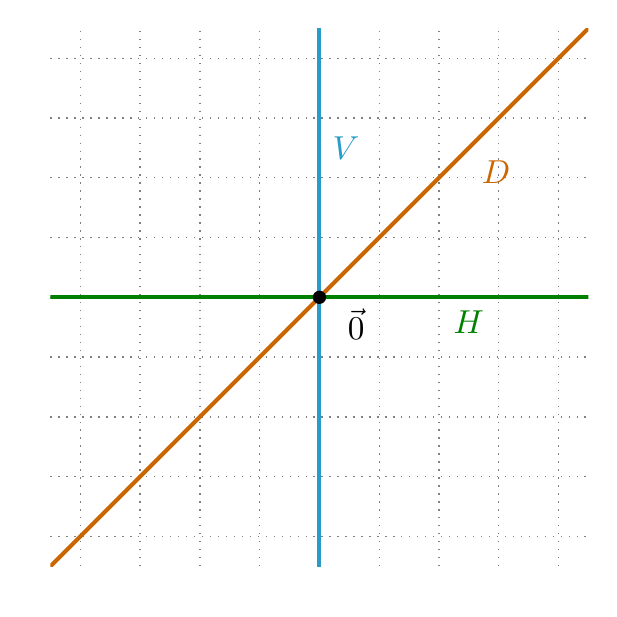
\begin{tikzpicture}[scale=1.2, >=latex]
    \begin{axis}[scale=1,
		    axis equal image,
		    axis line style={draw=none},
		    tick style={draw=none},
		    yticklabels={,,},
		    xticklabels={,,},
		 xmin=-4.5,
		 xmax=4.5,
		 ymin=-4.5,
		 ymax=4.5,
		 major grid style={dotted, gray},
                 xtick={-10,-9,...,10},
                 ytick={-10,-9,...,10},
                 grid=both,
		 anchor=origin]

	    \draw[Green, very thick] (-5,0) -- (5,0) node[near end, below] {$H$};
	    \draw[cyan!80!black, very thick] (0,-5) -- (0,5) node[near end, right] {$V$};
	    \draw[orange!80!black, very thick] (-5,-5) -- (5,5) node[near end, below right] {$D$};

	    \fill[fill=black] (0,0) circle[radius=2pt] node[below right, xshift=5pt] {\color{black}$\vec 0$};
    \end{axis}
\end{tikzpicture}
		\end{solution}
		\item $N=\Set*{\vec x\in\R^2 \given \vec x=t\mat{1\\1}\text{ for all }t\in\R}$.
				\begin{solution}[inline]
			$N=\Set{}$.
		\end{solution}

		\item $V\cup H$.
			\begin{solution}[inline]
			$V\cup H$ looks like a ``$+$'' going through the origin.
		\end{solution}
		\item $V\cap H$.
			\begin{solution}[inline]
				$V\cap H=\Set{\vec 0}$ is just the origin.
		\end{solution}
		\item Does $V\cup H=\R^2$?
			\begin{solution}
				No. $V\cup H$ does not contain $\mat{1\\1}$ while $\R^2$ does contain
				$\mat{1\\1}$.
			\end{solution}
	\end{parts}

	\bookonlynewpage
\section*{Vector Combinations}
	\vspace{-1em}

	\SavedDefinitionRender{LinearCombination}

	\question
	\label{ProbSkewBasis}
	\begin{annotation}
		\begin{goals}
			\Goal{Practice linear combinations.}

			The goal of this problem is to
			\begin{itemize}
				\item Practice using the formal term \emph{linear combination}.
				\item Foreshadow span.
			\end{itemize}
		\end{goals}

		\begin{notes}
			\begin{itemize}
				\item In 2, the question should arise: ``Is $3\vec v_1$
					a linear combination of $\vec v_1$ \emph{and}
					$\vec v_2$?'' Address this.
				\item Refer to the magic carpet ride for 5. You don't
					need to do a full proof.
			\end{itemize}
		\end{notes}
	\end{annotation}
	Let $\vec v_1=\mat{1\\1}$, $\vec v_2=\mat{1\\-1}$, and $\vec w=2\vec v_1+\vec v_2$.
	\begin{parts}
		\item Write $\vec w$ as a column vector. When $\vec w$ is written as a
			linear combination of $\vec v_1$ and $\vec v_2$, what are the
			coefficients of $\vec v_1$ and $\vec v_2$?
			\begin{solution}
				$\vec w=\mat{3\\2}$; the coefficients are $(2,1)$.
			\end{solution}
		\item Is $\mat{3\\3}$ a linear combination of $\vec v_1$ and $\vec v_2$?
			\begin{solution}[inline]
				Yes. $\mat{3\\3}=3\vec v_1+0\vec v_2$.
			\end{solution}

		\item Is $\mat{0\\0}$ a linear combination of $\vec v_1$ and $\vec v_2$?
			\begin{solution}[inline]
				Yes. $\vec 0=0\vec v_1+0\vec v_2$.
			\end{solution}
		\item Is $\mat{4\\0}$ a linear combination of $\vec v_1$ and $\vec v_2$?
			\begin{solution}[inline]
				Yes. $\mat{4\\0}=2\vec v_1+2\vec v_2$.
			\end{solution}
		\item Can you find a vector in $\R^2$ that isn't a linear combination of
		$\vec v_1$ and $\vec v_2$?
			\begin{solution}
				No. $\mat{1\\0}=\tfrac{1}{2}\vec v_1+\tfrac{1}{2}\vec v_2$ and
				$\mat{0\\1}=\tfrac{1}{2}\vec v_1-\tfrac{1}{2}\vec v_2$.
				Therefore
				\[
					\mat{a\\b}
					= a\mat{1\\0}+b\mat{0\\1}
					= a(\tfrac{1}{2}\vec v_1+\tfrac{1}{2}\vec v_2)
						+b(\tfrac{1}{2}\vec v_1-\tfrac{1}{2}\vec v_2)
					=(\tfrac{a+b}{2})\vec v_1+(\tfrac{a-b}{2})\vec v_2.
				\]
				Therefore any vector in $\R^2$ can be written as linear combinations
				of $\vec v_1$ and $\vec v_2$.
			\end{solution}
		\item Can you find a vector in $\R^2$ that isn't a linear combination of
			$\vec v_1$?
			\begin{solution}
				Yes. All linear combinations of $\vec v_1$ have equal $x$ and
				$y$ coordinates, therefore $\vec w=\mat{2\\1}$ is not a linear
				combination of $\vec v_1$.
			\end{solution}
	\end{parts}


	\bookonlynewpage
	\question
	\begin{annotation}
		\begin{goals}
			\Goal{Practice formal writing.}
		\end{goals}

		\begin{notes}
			\begin{itemize}
				\item Make everyone \emph{write}. They will think
					they can do it, but they will find it hard if
					they try.
			\end{itemize}
		\end{notes}
	\end{annotation}
	Recall the \emph{Magic Carpet Ride} task where the hover board could
	travel in the direction $\vec h=\mat{3\\1}$ and the magic carpet could
	move in the direction $\vec m=\mat{1\\2}$.
	\begin{parts}
		\item Rephrase the sentence \emph{``Gauss can be reached using just the
			magic carpet and the hover board''} using formal mathematical
			language.
			\begin{solution}
				Gauss's location can be written as a linear combination of
				$\vec m$ and $\vec h$.
			\end{solution}
		\item Rephrase the sentence \emph{``There is nowhere Gauss can hide
			where he is inaccessible by magic carpet and hover board''} using
			formal mathematical language.
			\begin{solution}
				Every vector in $\R^2$ can be written as a linear combination
				of $\vec m$ and	$\vec h$.
			\end{solution}
		\item Rephrase the sentence \emph{``$\R^2$ is the set of all linear
			combinations of $\vec h$ and $\vec m$''} using formal mathematical
			language.
			\begin{solution}
				$\R^2=\Set{\vec v\given \vec v=t\vec m+s\vec h\text{ for some }t,s\in \R}$.
			\end{solution}
	\end{parts}

\begin{module}
	\Title{Sets of Vectors, Lines \& Planes}

	In this module you will learn
	\begin{itemize}
		\item How to draw a set of vectors making an appropriate choice of when to use
			line segments and when to use dots to represent vectors.
		\item The \emph{vector form} of lines and planes, including how to determine
			the intersection of lines and planes in vector form.
		\item Restricted linear combinations and how to use them to represent common geometric
			objects (like line segments or polygons).
	\end{itemize}

	With a handle on vectors, we can now use them to describe some common geometric
objects: lines and planes.

\Heading{Lines}
Consider for a moment the line $\ell$ through the points $P$ and $Q$.  When $P,Q\in\R^2$, we
can describe $\ell$ with an equation of the form $y=mx+b$ (provided it isn't a vertical line), but if
$P,Q\in\R^3$, it's much harder to describe $\ell$ with an equation.  Using vectors
provides an easier way.

Let $\vec d=\overrightarrow{PQ}$ and consider the set of points (or vectors) $\vec x$ that can be expressed as
\[
	\vec x=t\vec d+P
\]
for $t\in \R$.  Geometrically, this is the set of all points we get by starting at $P$ and
displacing by some multiple of $\vec d$.  This is a line!


\begin{center}
	\begin{tikzpicture}
		\coordinate (A) at (1,1);
		\coordinate (B) at (3,2);
		\coordinate (D) at ($(B)-(A)$);
		\begin{axis}[
		    anchor=origin,
		    disabledatascaling,
		    xmin=-1,xmax=5,
		    ymin=-1,ymax=3,
		    x=1cm,y=1cm,
		    grid=both,
		    grid style={line width=.1pt, draw=gray!10},
		    %major grid style={line width=.2pt,draw=gray!50},
		    axis lines=middle,
		    minor tick num=0,
		    enlargelimits={abs=0.5},
		    axis line style={latex-latex},
		    ticklabel style={font=\tiny,fill=white},
		    xlabel style={at={(ticklabel* cs:1)},anchor=north west},
		    ylabel style={at={(ticklabel* cs:1)},anchor=south west}
		]

		\draw [Green,fill] (A) circle (1.5pt) node [below right] {$P$};
		\draw [Green,fill] (B) circle (1.5pt) node [below right] {$Q$};
		\draw[->,thick,myred!60!white] (A) -- (B) node [midway,below right,yshift=2pt] {$\vec d$};


		\end{axis}
		\foreach \x in {-1,5} {
			\draw [mypink,fill] ($(A)+\x/3*(D)$) circle (1.5pt) node [left] {\footnotesize$\tfrac{\x}{3}\vec d+P$};
		}
		\foreach \x in {-3,-2,4,6} {
			\draw [mypink,fill] ($(A)+\x/3*(D)$) circle (1.5pt);
		}
	\end{tikzpicture}
	\begin{tikzpicture}
		\coordinate (A) at (1,1);
		\coordinate (B) at (3,2);
		\coordinate (D) at ($(B)-(A)$);
		\begin{axis}[
		    anchor=origin,
		    disabledatascaling,
		    xmin=-1,xmax=5,
		    ymin=-1,ymax=3,
		    x=1cm,y=1cm,
		    grid=both,
		    grid style={line width=.1pt, draw=gray!10},
		    %major grid style={line width=.2pt,draw=gray!50},
		    axis lines=middle,
		    minor tick num=0,
		    enlargelimits={abs=0.5},
		    axis line style={latex-latex},
		    ticklabel style={font=\tiny,fill=white},
		    xlabel style={at={(ticklabel* cs:1)},anchor=north west},
		    ylabel style={at={(ticklabel* cs:1)},anchor=south west}
		]

		\draw [Green,fill] (A) circle (1.5pt) node [below right] {$P$};
		\draw [Green,fill] (B) circle (1.5pt) node [below right] {$Q$};
		\draw[->,thick,myred!60!white] (A) -- (B) node [midway,below right,yshift=2pt] {$\vec d$};

		\end{axis}

		\foreach \x in {-3,-2,-1,0,4,5,6} {
			\draw [->, gray!50!white] (0,0) -- ($(A)+\x/3*(D)$);
		}
		\foreach \x in {-1,5} {
			\draw [mypink,fill] ($(A)+\x/3*(D)$) circle (1.5pt) node [left] {\footnotesize$\tfrac{\x}{3}\vec d+P$};
		}
		\foreach \x in {-3,-2,4,6} {
			\draw [mypink,fill] ($(A)+\x/3*(D)$) circle (1.5pt);
		}
	\end{tikzpicture}
\end{center}
We simultaneously interpret this line as a set of points (the points that make up
the line) and as a set of vectors 
rooted at the origin (the vectors pointing from the origin to the line).
Note that sometimes we draw vectors as directed line segments.
Other times, drawing drawing vectors as line segments makes
it hard to see what is going on, and so it is better to draw
each vector by marking only its ending point.

Which picture below do you think best represents $\ell$?
\begin{center}
	\begin{tikzpicture}
		\coordinate (A) at (1,1);
		\coordinate (B) at (3,2);
		\coordinate (D) at ($(B)-(A)$);
		\begin{axis}[
		    anchor=origin,
		    disabledatascaling,
		    xmin=-1,xmax=5,
		    ymin=-1,ymax=3,
		    x=1cm,y=1cm,
		    grid=both,
		    grid style={line width=.1pt, draw=gray!10},
		    %major grid style={line width=.2pt,draw=gray!50},
		    axis lines=middle,
		    minor tick num=0,
		    enlargelimits={abs=0.5},
		    axis line style={latex-latex},
		    ticklabel style={font=\tiny,fill=white},
		    xlabel style={at={(ticklabel* cs:1)},anchor=north west},
		    ylabel style={at={(ticklabel* cs:1)},anchor=south west}
		]

		\node[above right] at (0,3) {~Vectors in $\ell$ as dots};
		\draw [mypink, thick] ($(A)-3*(D)$) -- ($(A)+3*(D)$);
		\end{axis}
	\end{tikzpicture}
	\begin{tikzpicture}
		\coordinate (A) at (1,1);
		\coordinate (B) at (3,2);
		\coordinate (D) at ($(B)-(A)$);
		\begin{axis}[
		    anchor=origin,
		    disabledatascaling,
		    xmin=-1,xmax=5,
		    ymin=-1,ymax=3,
		    x=1cm,y=1cm,
		    grid=both,
		    grid style={line width=.1pt, draw=gray!10},
		    %major grid style={line width=.2pt,draw=gray!50},
		    axis lines=middle,
		    minor tick num=0,
		    enlargelimits={abs=0.5},
		    axis line style={latex-latex},
		    ticklabel style={font=\tiny,fill=white},
		    xlabel style={at={(ticklabel* cs:1)},anchor=north west},
		    ylabel style={at={(ticklabel* cs:1)},anchor=south west}
		]
			\node[above right] at (0,3) {~Vectors in $\ell$ as arrows from $(0,0)$};
		\end{axis}

		\foreach \x in {-8,...,14} {
			\draw [->, mypink] (0,0) -- ($(A)+\x/6*(D)$);
		}
	\end{tikzpicture}
\end{center}


\begin{emphbox}[Takeaway]
	When drawing a picture depicting several vectors, make an appropriate choice (arrows, dots, or
	a mix) so that the picture is clear.
\end{emphbox}

The line $\ell$ described above can be written in set-builder notation
as:
\[
	\ell=\Set{\vec x\given \vec x=t\vec d+P\text{ for some }t\in \R}.
\]
Notice that in set-builder notation, we write ``for some $t\in \R$.'' Make sure you
understand why replacing ``for some $t\in\R$'' with ``for
all $t\in \R$'' would be incorrect.

Writing lines with set-builder notation all the time can be overkill,
so we will allow ourselves to describe lines in a shorthand called \emph{vector form}\footnote{
	$y=mx+b$ form of a line is also shorthand.  The line $\ell$ described by the equation
	$y=mx+b$ is actually the set $\Set{(x,y)\in\R^2\given y=mx+b}$.
}.

\SavedDefinitionRender{VectorFormofaLine}

We can also use coordinates when writing a line in vector form. For example,
\[
	\mat{x\\y}=t\mat{d_1\\d_2}+\mat{p_1\\p_2}
\]
corresponds to the line passing through $\mat{p_1\\p_2}$ with $\mat{d_1\\d_2}$ as a direction vector.

The ``$t$'' that appears in a vector form is called the \emph{parameter variable}, and for this
reason, some textbooks use the term \emph{parametric form} in place of ``vector form''. 

Writing a line in vector form only requires a point on the line and a direction for the line.
Thus, converting to vector form from another form is straightforward.
\begin{example}
	Find vector form of the line $\ell\subseteq\R^2$ with equation $y=2x+3$.

	First, we find two
	points on the line.  By guess-and-check we see $P=(0,3)$ and $Q=(1,5)$ are on $\ell$.
	Thus, a direction vector for $\ell$ is given by
	\[
		\vec d = (1,5)-(0,3)=(1,2).
	\]
	We may now express $\ell$ in vector form as
	\[
		\vec x=t\vec d+P
	\]
	or, in components,
	\[
		\mat{x\\y} = t\mat{1\\2}+\mat{0\\3}.
	\]
\end{example}

It's important to note that when we write a line in vector form, it is a \emph{specific shorthand} notation.
If we augment the notation, we no longer have written a line in ``vector form''.

\begin{example} Let $\ell$ and let $\vec d$ be a direction vector for $\ell$ and let $\vec p\in \ell$
	be a point on $\ell$. Writing
	\[
		\vec x=t\vec d+\vec p
	\]
	or 
	\[
		\vec x=t\vec d+\vec p\quad\text{ where }\quad t\in \R
	\]
	specifies $\ell$ in vector form and are both shorthands for $\Set{\vec x\given
	\vec x=t\vec d+\vec p\text{ for some }t\in \R}$. But,
	\[
		\vec x=t\vec d+\vec p\quad\text{ for some }\quad t\in \R
	\]
	and
	\[
		\vec x=t\vec d+\vec p\quad\text{ for all }\quad t\in \R
	\]
	are logical statements about the vectors $\vec x$, $\vec d$, and
	$\vec p$. These statements are either true or false; they do \emph{not} 
	specify $\ell$ in vector form.

	Similarly, the statement
	\[
		\ell = t\vec d+\vec p
	\]
	is mathematically nonsensical and does not specify $\ell$ in vector form. (On the
	left is a \emph{set} and on the right is a \emph{vector}!)

\end{example}

But, why is vector form useful? For starters, every line can be expressed in vector form 
(you cannot write a vertical line in $y=mx+b$ form, and in $\R^3$, you would need two linear equations
to represent a line). But, the most useful thing about expressing a line in vector form is that
you can easily generate points on that line.

Suppose $\ell$ can be represented in vector form as $\vec x=t\vec d+\vec p$.
Then, for every $t\in \R$, the vector $t\vec d +\vec p\in\ell$. Not only that, but as $t$ ranges over
$\R$, all points on $\ell$ are ``traced out''. Thus, we can find points on $\ell$ without having to ``solve''
any equations.

The downside to using vector form is that it is not unique. There are multiple direction vectors and multiple points
for every line.  Thus, merely by looking at the vector equation for two lines, it can be hard to tell if
they're equal.

For example,
\[
	\mat{x\\y} = t\mat{1\\2}+\mat{0\\3},\qquad
	\mat{x\\y} = t\mat{2\\4}+\mat{0\\3},\quad\text{and}\quad
	\mat{x\\y} = t\mat{1\\2}+\mat{1\\5}
\]
all represent the same line.  In the second equation, the direction vector is parallel but scaled, and in
the third equation, a different point on the line was chosen.

Recall that in vector form, the variable $t$ is called the \emph{parameter variable}.  It is an instance of
a \emph{dummy variable}. In other words, $t$ is a placeholder---just because ``$t$'' appears in two different vector
forms, doesn't mean it's the same quantity.

To drive this point home, we need to remember that vector
form is shorthand for a set described in set-builder notation.

\bigskip
Let $\vec d_1,\vec d_2\neq\vec 0$ and $\vec p_1,\vec p_2$ be vectors and define the lines
\[
	\ell_1=\Set{\vec x\given \vec x=t\vec d_1+\vec p_1\text{ for some }t\in\R}
\]
\[
	\ell_2=\Set{\vec x\given \vec x=t\vec d_2+\vec p_2\text{ for some }t\in\R}.
\]
These lines have vector forms $\vec x=t\vec d_1+\vec p_1$ and $\vec x=t\vec d_2+\vec p_2$.
However, declaring that $\ell_1=\ell_2$ if and only if $t\vec d_1+\vec p_1=t\vec d_2+\vec p_2$
does \emph{not} make sense.   Instead, as per the definition, $\ell_1=\ell_2$ if $\ell_1\subseteq\ell_2$ and $\ell_2\subseteq\ell_1$.
If $\vec x\in\ell_1$ then $\vec x=t\vec d_1+\vec p_1$ for some $t\in\R$.  If $\vec x\in\ell_2$
then $\vec x=t\vec d_2+\vec p_2$ for some \emph{possibly different} $t\in \R$.  This can get
confusing really quickly.  The easiest way to avoid confusion is to use different parameter variables 
when comparing different vector forms.

\begin{example}
	Determine if the lines $\ell_1$ and $\ell_2$, given in vector form as 
	\[
		\vec x=t\mat{1\\1}+\mat{2\\1}\qquad\text{and}\qquad
		\vec x=t\mat{2\\2}+\mat{4\\3},
	\]
	are the same line.  
	
	To determine this, we need to figure out if $\vec x\in\ell_1$
	implies $\vec x\in \ell_2$ and if $\vec x\in\ell_2$ implies $\vec x\in\ell_1$.

	If $\vec x\in\ell_1$, then $\vec x=t\mat{1\\1}+\mat{2\\1}$ for some $t\in\R$.  If
	$\vec x\in\ell_2$, then $\vec x=s\mat{2\\2}+\mat{4\\3}$ for some $s\in \R$.  Thus if
	\[
		t\mat{1\\1}+\mat{2\\1} = \vec x = s\mat{2\\2}+\mat{4\\3}
	\]
	always has a solution, $\ell_1=\ell_2$.  Moving everything to one side we see
	\begin{align*}
		\vec 0 = \mat{4\\3}-\mat{2\\1} + s\mat{2\\2}-t\mat{1\\1}
		&=\mat{2\\2}+s\mat{2\\2}-t\mat{1\\1}\\
		&=(s+1)\mat{2\\2}-\tfrac{t}{2}\mat{2\\2}\\
		&= (s+1-\tfrac{t}{2})\mat{2\\2}.
	\end{align*}
	This has a solution whenever $0=s+1-t/2$.  Since for every $t\in\R$ we can find an $s\in\R$ satisfying
	this equation
	and for every $s\in \R$ we can find a $t\in \R$ satisfying this equation, we know $\ell_1=\ell_2$.
\end{example}


\Heading{Vector Form in Higher Dimensions}
The geometry of lines in space ($\R^3$ and above) is a bit more complicated than that of lines
in the plane.  Lines in the plane either intersect or are parallel.
In space,  we have to be a more careful about what we mean by
``parallel lines,'' since lines with entirely different directions can
still fail to intersect\footnote{ Recall that in Euclidean geometry
two lines are defined to be parallel if they coincide or never intersect.}.

\begin{center}
  \begin{tikzpicture}
    \begin{axis}[grid=major,view={20}{40},z buffer=sort,
	    zmin=0,
	    xticklabels={,,}, yticklabels={,,}, zticklabels={,,}
	    ]
	    \addplot3 [no marks,orange,ultra thick] coordinates {(0,10,10) (20,10,30)};
	    \addplot3 [no marks,orange,dashed, thick] coordinates {(0,10,0) (20,10,0)};
	    \addplot3 [no marks,mypink,ultra thick] coordinates {(0,0,20) (20,20,0)};
	    \addplot3 [no marks,mypink,dashed, thick] coordinates {(0,0,0) (20,20,0)};
	%\addplot3[domain=4:30,samples=80,samples y=0,mark=none,orange, opacity=0.5,ultra thick]
	%    ({x},{118.89/x},{2*x});
    \end{axis}
  \end{tikzpicture}
\end{center}

\begin{example}
Consider the lines described by
\begin{align*}
\vec x &= t( 1, 3, -2 ) + ( 1, 2, 1 ) \\
\vec x &= t( -2, -6, 4) + ( 3, 1, 0 ).
\end{align*}
They have parallel directions since $( -2, -6, 4 ) = -2( 1, 3,-2 )$.
Hence, in this case, we say the lines are \emph{parallel}\index{parallel lines}.  (How can
we be sure the lines are not the same?)
\end{example}

\begin{example}
Consider the lines described by
\begin{align*}
	\vec x &= t(1, 3, -2 ) + ( 1, 2, 1 ) \\
	\vec x &= t( 0, 2, 3) + ( 0, 3, 9 ).
\end{align*}
They are not parallel because neither of the direction
vectors is a multiple
of the other.  They may or may not intersect.  (If they don't,
	we say the lines are \emph{skew}\index{skew lines}.)  How can we find out?
	Mirroring our earlier approach,
	we can set their equations equal and see if we can solve for the point
	of intersection \emph{after ensuring we give their parametric variables
	different names}.   We'll keep one parametric variable named $t$ and name the
	other one $s$.  Thus, we want
\[
\vec x = t( 1, 3, -2 ) + ( 1, 2, 1 ) =
s( 0, 2, 3) + ( 0, 3, 9 ),
\]
which after collecting terms yields
\[
    ( t + 1, 3t + 2, -2t + 1 ) = ( 0, 2s + 3, 3s + 9).
\]
Picking out the components yields three equations
\begin{align*}
    t + 1 &= 0 \\
    3t +2 &= 2s + 3 \\
    -2t + 1 &=  3s + 9
\end{align*}
in 2 unknowns  $s$ and $t$.  This is an {\it overdetermined\/}
system, and it may or may not have a consistent solution.
The first two equations yield $t = -1$  and $s = -2$.  Putting
these values in the last equation yields $(-2)(-1) + 1 = 3(-2) + 9$,
which is indeed true.
Hence, the equations are consistent, and the lines
intersect.   To find the point of intersection, put $t = -1$
in the equation for the first line (or
$s = -2$ in that for the second) to obtain  $( 0, -1, 3 )$.
\end{example}

\Heading{Planes}

Any two distinct points define a line.  To define a plane, we
need three points.  But there's a caveat: the three points cannot
be on the same line, otherwise they'd define a line
and not a plane.  Let $A,B,C\in\R^3$ be three points that are not
collinear and let $\mathcal P$ be the plane that passes through $A$,
$B$, and $C$.

Just like lines, planes have direction vectors.  For $\mathcal P$, both
$\vec d_1=\overrightarrow{AB}$ and $\vec d_2=\overrightarrow{AC}$ are direction
vectors for $\mathcal P$.  Of course, $\vec d_1$, $\vec d_2$ and their multiples
are not the only direction vectors for $\mathcal P$. There are infinitely many more, including
$\vec d_1+\vec d_2$, and $\vec d_1-7\vec d_2$, and so on.  However, since a plane
is a \emph{two}-dimensional object, we only need two different direction vectors to describe it.

Like lines, planes have a vector form.  Using the direction vectors $\vec d_1=\overrightarrow{AB}$ and 
$\vec d_2=\overrightarrow{AC}$,
the plane $\mathcal P$ can be written in vector form as
\[
	\mat{x\\y\\z} = t\vec d_1+s\vec d_2+A.
\]
\begin{center}
  \begin{tikzpicture}
    \begin{axis}[grid=major,view={20}{40},z buffer=sort,
	    %zmin=0,
	    xticklabels={,,}, yticklabels={,,}, zticklabels={,,}
	    ]
		\addplot3 [data cs=cart,surf,domain=-10:10,samples=2, opacity=0.5]
		{x+y};
		\coordinate (A) at (axis cs:-3,-3,-6);
		\coordinate (B) at (axis cs:3,4,7);
		\coordinate (C) at (axis cs:-4,4,0);

		\draw [mypink,fill] (A) circle (1.5pt) node [below right] {$A$};
		\draw [->, thick] (A) -- (B) node [midway,below right] {$\vec d_1$};
		\draw [->, thick] (A) -- (C) node [midway,above left] {$\vec d_2$};
    \end{axis}
  \end{tikzpicture}
\end{center}

\SavedDefinitionRender{VectorFormofaPlane}

\begin{example}
	Describe the plane $\mathcal P\subseteq \R^3$ with equation $z=2x+y+3$ in vector form.

	To describe $\mathcal P$ in vector form, we need a point on $\mathcal P$ and two direction
	vectors for $\mathcal P$. By guess-and-check, we see the points
	\[
		A=\mat{0\\0\\3}\qquad B=\mat{1\\0\\5}\qquad C=\mat{0\\1\\4}
	\]
	are all on $\mathcal P$. Thus
	\[
		\vec d_1=B-A=\mat{1\\0\\2}\qquad \text{and}\qquad
		\vec d_2=C-A=\mat{0\\1\\1}
	\]
	are both direction vectors for $\mathcal P$.  Therefore, we can express $\mathcal P$ in vector
	form as
	\[
		\vec x=t\vec d_1+s\vec d_2+A=t\mat{1\\0\\2}+s\mat{0\\1\\1}+\mat{0\\0\\3}.
	\]
\end{example}


\begin{example}
	Find the line of intersection between $\mathcal P_1$ and $\mathcal P_2$ where 
	$\mathcal P_1$ and $\mathcal P_2$ are expressed in vector form as ...

	XXX Finish
\end{example}

\Heading{Restricted Linear Combinations}

Using vectors, we can describe more than just lines and planes---we can describe 
all sorts of geometric objects.

Recall that when we write $\vec x=t\vec d+\vec p$
to describe the line $\ell$,
what we mean is
\[
	\ell=\Set{\vec x\given \vec x=t\vec d+\vec p\text{ for some }t\in \R}.
\]
The line $\ell$ stretches off infinitely in both directions. But, what if we wanted
to describe just a part of $\ell$? We can do this by placing additional restrictions
on $t$.
For example, consider the ray $R$
and the line segment $S$:
\begin{align*}
	R&=\Set{\vec x\given \vec x=t\vec d+\vec p\text{ for some }t\geq 0}\\
	S&=\Set{\vec x\given \vec x=t\vec d+\vec p\text{ for some }t\in [0,2]}
\end{align*}

\begin{center}
	\begin{tikzpicture}
		\begin{axis}[
		    anchor=origin,
		    disabledatascaling,
		    xmin=-1,xmax=4,
		    ymin=-1,ymax=3,
		    x=1cm,y=1cm,
		    grid=both,
		    grid style={line width=.1pt, draw=gray!10},
			xtick={0,1,2,3,4},
		    %major grid style={line width=.2pt,draw=gray!50},
		    axis lines=middle,
		    minor tick num=0,
		    enlargelimits={abs=0.5},
		    axis line style={latex-latex},
		    ticklabel style={font=\tiny,fill=white},
		    xlabel style={at={(ticklabel* cs:1)},anchor=north west},
		    ylabel style={at={(ticklabel* cs:1)},anchor=south west}
		]

			\draw [mypink, very thick] (0,0) -- (5,3) node[midway, below right] {$R$};
			\draw [black!70!white, thick,dashed, ->, yshift=.15cm] (0,0) -- (5/5,3/5) node[midway, above] {$\vec d$};
		\end{axis}
			\node[above right] at (0,3) {~The ray $R$};
	\end{tikzpicture}
	~~~~
	\begin{tikzpicture}
		\begin{axis}[
		    anchor=origin,
		    disabledatascaling,
		    xmin=-1,xmax=4,
		    ymin=-1,ymax=3,
			xtick={0,1,2,3,4},
		    x=1cm,y=1cm,
		    grid=both,
		    grid style={line width=.1pt, draw=gray!10},
		    %major grid style={line width=.2pt,draw=gray!50},
		    axis lines=middle,
		    minor tick num=0,
		    enlargelimits={abs=0.5},
		    axis line style={latex-latex},
		    ticklabel style={font=\tiny,fill=white},
		    xlabel style={at={(ticklabel* cs:1)},anchor=north west},
		    ylabel style={at={(ticklabel* cs:1)},anchor=south west}
		]
			\draw [mygreen, very thick] (0,0) -- (10/5,6/5) node[midway, below right] {$S$};
			\draw [black!70!white, thick,dashed, ->, yshift=.15cm] (0,0) -- (5/5,3/5) node[midway, above] {$\vec d$};
		\end{axis}
			\node[above right] at (0,3) {~The line segment $S$};
	\end{tikzpicture}
\end{center}

We can also make polygons by adding restrictions to the vector form of a plane. Let
$\vec a=\mat{2\\1}$ and $\vec b=\mat{-1\\1}$ and consider the unit square $U$ and
the parallelogram $P$ defined by
\begin{align*}
	U&=\Set{\vec x\given \vec x=t\xhat+s\yhat\text{ for some }t,s\in [0,1]}\\
	P&=\Set{\vec x\given \vec x=t\vec a+s\vec b\text{ for some }t\in [0,1]\text{ and }s\in[-1,1]}
\end{align*}

\begin{center}
	\begin{tikzpicture}
		\begin{axis}[
		    anchor=origin,
		    disabledatascaling,
		    xmin=-2,xmax=3,
		    ymin=-1,ymax=2,
			xtick={-2,...,3},
			ytick={-2,...,3},
		    x=1cm,y=1cm,
		    grid=both,
		    grid style={line width=.1pt, draw=gray!10},
		    %major grid style={line width=.2pt,draw=gray!50},
		    axis lines=middle,
		    minor tick num=0,
		    enlargelimits={abs=0.5},
		    axis line style={latex-latex},
		    ticklabel style={font=\tiny,fill=white},
		    xlabel style={at={(ticklabel* cs:1)},anchor=north west},
		    ylabel style={at={(ticklabel* cs:1)},anchor=south west}
		]

			\fill [mypink, opacity=.3] (0,0) -- (1,0) -- (1,1) node[midway, right, opacity=1] {$U$} -- (0,1) -- cycle;
			\draw [black!70!white, thick,dashed, ->, yshift=-.15cm] (0,0) -- (1,0) node[midway, below] {$\xhat$};
			\draw [black!70!white, thick,dashed, ->, xshift=-.15cm] (0,0) -- (0,1) node[midway, left] {$\yhat$};
		\end{axis}
			\node[above right] at (0,2) {~The unit square $U$};
	\end{tikzpicture}
	~~~~
	\begin{tikzpicture}
		\begin{axis}[
		    anchor=origin,
		    disabledatascaling,
		    xmin=-2,xmax=3,
		    ymin=-1,ymax=2,
			xtick={-2,...,3},
			ytick={-2,...,3},
		    x=1cm,y=1cm,
		    grid=both,
		    grid style={line width=.1pt, draw=gray!10},
		    %major grid style={line width=.2pt,draw=gray!50},
		    axis lines=middle,
		    minor tick num=0,
		    enlargelimits={abs=0.5},
		    axis line style={latex-latex},
		    ticklabel style={font=\tiny,fill=white},
		    xlabel style={at={(ticklabel* cs:1)},anchor=north west},
		    ylabel style={at={(ticklabel* cs:1)},anchor=south west}
		]
			\fill [mygreen, opacity=.3] (1,2) -- (3,0) -- (1,-1) node[midway, below right, opacity=1] {$P$} -- (-1,1) -- cycle;
			\draw [black!70!white, thick,dashed, ->] (0,0) -- (2,1) node[midway, below right] {$\vec a$};
			\draw [black!70!white, thick,dashed, ->] (0,0) -- (-1,1) node[midway, left, yshift=-3pt] {$\vec b$};
		\end{axis}
			\node[above right] at (0,2) {~The parallelogram $P$};
	\end{tikzpicture}
\end{center}

Each set so far is a set of linear combinations, and we 
have made different shapes by restricting the coefficients of those linear
combinations. There are two ways of restricting linear combinations that arise
up often enough to get their own names.

\SavedDefinitionRender{NonnegativeConvexLinearCombinations}

You can think of a non-negative linear combinations as vector you can arrive at by
only displacing ``forward'' along your vectors.
Convex linear combinations can be thought of as weighted averages of vectors (the average of $\vec v_1,\ldots,
\vec v_n$ would be the convex linear combination with coefficients $\alpha_i=\frac{1}{n}$). 
A convex linear combination
of two vectors gives a point on the line segment connecting them. 

\begin{example}
	Let $\vec a=\mat{2\\1}$ and $\vec b=\mat{-1\\1}$ and define
	\begin{align*}
		A&=\Set{\vec x\given \vec x\text{ is a convex linear combination of }\vec a\text{ and }\vec b}\\
		&=\Set{\vec x\given \vec x=\alpha\vec a+(1-\alpha)\vec b\text{ for some }\alpha\in [0,1]}.
	\end{align*}
	Draw $A$.

	XXX Finish

	XXX Figure
\end{example}


	
\end{module}
\begin{lesson}
	\Title{Restricted Linear Combinations, Lines}

	\Heading{Textbook} Section 1.2

	\Heading{Objectives}
	\begin{itemize}
		\item Read and digest a new definition.

		\item Use pictures to explore a new concept.

		\item Convert from an equation-representation of a line to a set-representation.
	\end{itemize}

	\Heading{Motivation} Part of doing math in the world is reading and understanding
	other people's definitions. Most students will not have heard of non-negative
	linear combinations or convex linear combinations. This is a chance for them
	to read and try to understand these formal definitions. They will need to
	draw pictures to get an intuition about what these concepts mean.

	These concepts are useful in their own right, and in particular, convex linear
	combinations can be used to describe line segments. Adding these definitions
	to a student's toolbox serves the goal of \emph{being able to describe
	the world with mathematics}.

	To that end, we start working with lines. Lines are something students have
	used since grade school, but they worked with them in $y=mx+b$ form which
	is only applicable in $\R^{2}$. We want to convert this representation
	into vector form and set-based descriptions which apply to all
	dimensions.

\end{lesson}

	\displayonlynewpage
	\SavedDefinitionRender{NonnegativeConvexLinearCombinations}

	\question
	\begin{annotation}
		\begin{goals}
			\Goal{Geometric meaning of \emph{non-negative} and \emph{convex}
			linear
			combinations.}

			The goal of this problem is to
			\begin{itemize}
				\item Read and apply the definition of non-negative and convex
					linear combinations.
				\item Gain geometric intuition for non-negative and convex linear
					combinations.
				\item Learn how to describe line segments using
					convex linear combinations.
			\end{itemize}
		\end{goals}

		\begin{notes}
			\begin{itemize}
				\item This question is about reading and applying;
					emphasize that before they start.
				\item The geometry won't be obvious. Ask them to \emph{draw} specific
					linear combinations (e.g., $(1/2,1/2)$) to get an idea.
				\item They know $\vec a$ and $\vec b$ span all vectors from problem \ref{ProbSkewBasis}.
				\item In part 1, they will forget $\vec a$ and $\vec b$ are linear combinations of themselves.
				\item Part 2 (b) highlights a degeneracy that will come up again when discussing linear independence
					and dependence. Explain how the picture for non-negative linear combinations
					almost always looks one way, but this case is an exception.
			\end{itemize}
		\end{notes}
	\end{annotation}
	Let
	\[
		\vec a=\mat{1\\1} \qquad \vec b=\mat{-1\\1}\qquad \vec c=\mat{0\\1}\qquad\vec d=\mat{0\\2}\qquad\vec e=\mat{-1\\-1}.
	\]
	\begin{parts}
		\item Out of $\vec a$, $\vec b$, $\vec c$, $\vec d$, and $\vec e$, which
			vectors are
			\begin{enumerate}
				\item linear combinations of $\vec a$ and $\vec b$?
				\begin{solution}[inline]
					All of them, since any vector in $\R^2$ can be written as a linear combination
					of $\vec a$ and $\vec b$.
				\end{solution}

				\item non-negative linear combinations of $\vec a$ and $\vec b$?
				\begin{solution}[inline]
					$\vec a$, $\vec b$, $\vec c$, $\vec d$.
				\end{solution}

				\item convex linear combinations of $\vec a$ and $\vec b$?
				\begin{solution}[inline]
					$\vec a$, $\vec b$, $\vec c$.
				\end{solution}
			\end{enumerate}

		\item If possible, find two vectors $\vec u$ and $\vec v$ so that
			\begin{enumerate}
				\item $\vec a$ and $\vec c$ are non-negative linear combinations
					of $\vec u$ and $\vec v$ but $\vec b$ is not.
				\begin{solution}
					Let $\vec u=\vec a$ and $\vec v=\vec c$.
				\end{solution}

				\item $\vec a$ and $\vec e$ are non-negative linear combinations
					of $\vec u$ and $\vec v$.
				\begin{solution}
					Let $\vec u=\vec a$ and $\vec v=\vec e$.
				\end{solution}

				\item $\vec a$ and $\vec b$ are non-negative linear combinations
					of $\vec u$ and $\vec v$ but $\vec d$ is not.
				\begin{solution}
					Impossible. If $\vec a$ and $\vec b$ are non-negative
					linear combinations of $\vec u$ and $\vec v$, then every non-negative
					linear combination of $\vec a$ and $\vec b$ is also a non-negative
					linear combination of $\vec u$ and $\vec v$. And, we already concluded that
					$\vec d$ is a non-negative linear combination of $\vec a$ and $\vec b$.
				\end{solution}

				\item $\vec a$, $\vec c$, and $\vec d$ are convex linear
					combinations of $\vec u$ and $\vec v$.
				\begin{solution}
					Impossible. Convex linear combinations all lie on the same line segment,
					but $\vec a$, $\vec c$, and $\vec d$ are not collinear.
				\end{solution}
			\end{enumerate}Otherwise, explain why it's not possible.
	\end{parts}

	\displayonlynewpage
	\bookonlynewpage
\section*{Lines and Planes}

	\question
	\begin{annotation}
		\begin{goals}
			\Goal{Link prior knowledge to new notation/concepts.}

			The goal of this problem is to
			\begin{itemize}
				\item Convert between $y=mx+b$ form of a line and
					the set-builder definition of the same line.
				\item Think about lines in terms of vectors rather
					than equations.
			\end{itemize}
		\end{goals}

		\begin{notes}
			\begin{itemize}
				\item This question is foreshadowing for vector form of a line.
				\item In part 3, some will draw $\vec d$ from the origin and
					some will draw it on the line. Both are fine, but make
					sure they understand that $\vec d\notin L$ by the end of
					part 4.
			\end{itemize}
		\end{notes}
	\end{annotation}
	Let $L$ be the set of points $(x,y)\in\R^2$ such that $y=2x+1$.
	\begin{parts}
		\item Describe $L$ using set-builder notation.
			\begin{solution}
				$\Set*{\vec v\in\R^2 \given \vec v=\matc{t\\2t+1}\text{ for some } t\in\R}$\\
				or
				$\Set*{\mat{x\\y}\in\R^2 \given y=2x+1}$
				or
				$\Set*{\matc{t\\2t+1}\in\R^2 \given t\in\R}$
			\end{solution}
		\item Draw $L$ as a subset of $\R^2$.
		\item Add the vectors $\vec a=\mat{-1\\-1}$, $\vec b=\mat{1\\3}$ and
			$\vec d=\vec b-\vec a$ to your drawing.
			\begin{solution}
				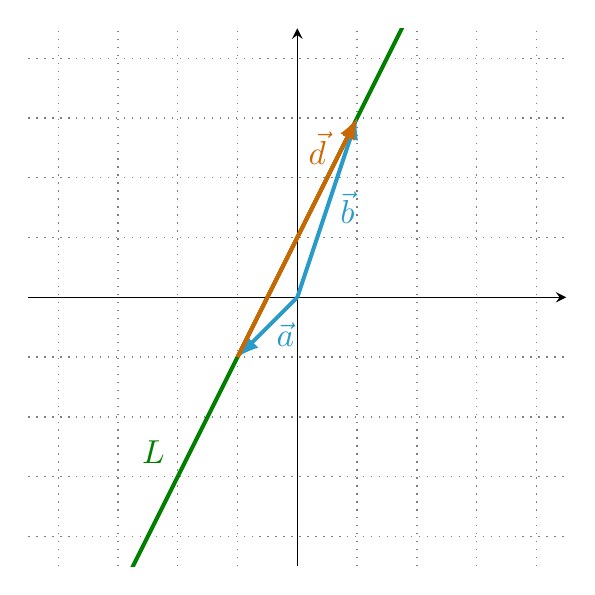
\begin{tikzpicture}[scale=1.2, >=latex]
			    \begin{axis}[scale=1,
					    axis equal image,
					    axis lines=middle,
					    axis line style = {black},
					    tick style={draw=none},
					    yticklabels={,,},
					    xticklabels={,,},
					 xmin=-4.5,
					 xmax=4.5,
					 ymin=-4.5,
					 ymax=4.5,
					 major grid style={dotted, gray},
					 xtick={-10,-9,...,10},
					 ytick={-10,-9,...,10},
					 grid=both,
					 anchor=origin]

				    \draw[Green, very thick] (-5,-9) -- (5,11) node[pos=.3, above left] {$L$};
				    \draw[cyan!80!black, very thick, ->] (0,0) -- (-1,-1) node[pos=.2, below] {$\vec a$};
				    \draw[cyan!80!black, very thick, ->] (0,0) -- (1,3) node[pos=.5, right] {$\vec b$};
				    \draw[orange!80!black, very thick, ->] (-1,-1) -- (1,3) node[near end, above, xshift=-3pt] {$\vec d$};

			    \end{axis}
				\end{tikzpicture}
			\end{solution}
		\item Is $\vec d\in L$? Explain.
			\begin{solution}
				No. $\vec d=\mat{2\\4}$ and so its entries don't satisfy $y=2x+1$.
			\end{solution}
		\item For which $t\in\R$ is it true that $\vec a+t\vec d\in L$? Explain using your picture.
			\begin{solution}
				$\vec a +t\vec d\in L$ for any $t\in \R$. We can see this because if we start at the
				vector $\vec a$ and the displace by $t\vec d$, we will always be on the line $L$.
			\end{solution}
	\end{parts}

\begin{lesson}
	\Title{Vector Form of Lines, Intersecting Lines}

	\Heading{Textbook}
	Section 1.2

	\Heading{Objectives}
	\begin{itemize}
		\item Fluency with vector form of a line in $\R^2$ and $\R^3$.
		\item Recognize that vector form of a line is not unique.
		\item Find the intersection of two lines in vector form.
	\end{itemize}

	\Heading{Motivation}
	A single linear equation cannot describe a line in more than two dimensions.
	One way to describe a line that works in all dimensions is vector form, which
	is a shorthand for a particular set. Vector form has the upside that it makes it easy
	to produce points on a line, but it has the downside that it is not unique.

	\begin{annotation}
		\begin{notes}
			Giving a proper definition of vector form of a line is awkward and
			shouldn't be the focus. For vector form, that they ``know it when they see it''
			and can ``produce it'' is good enough. (This is in contrast to other definitions
			which they must be able to correctly state).
		\end{notes}
	\end{annotation}
	Vector form works because a line in any dimension can be defined by two
	points or, equivalently, a point and a direction. Though we don't yet have
	a systematic way to write solutions to a system of linear equations,
	if we have a system representing a line, all we need to do is guess two
	solutions to that system to find vector form of the line.


	\begin{annotation}
		\begin{notes}
			The biggest stumbling block for finding the intersection of two lines
			in vector form will be choosing different dummy variables before
			setting the lines equal.
		\end{notes}
	\end{annotation}
	One thing vector form makes difficult is finding intersections, but intersections
	can be turned into just another algebra problem involving a system of equations.

\end{lesson}

	\bookonlynewpage
	\SavedDefinitionRender{VectorFormofaLine}

	\question
	\begin{annotation}
		\begin{goals}
			\Goal{Practice with vector form.}

			The goal of this problem is to
			\begin{itemize}
				\item Express lines in $\R^2$ and $\R^3$ in
					vector form.
				\item Produce direction vectors by subtracting two points
					on a line.
				\item Recognize vector form is not unique.
			\end{itemize}
		\end{goals}

		\begin{notes}
			\begin{itemize}
				\item If students get stuck on part 1, ask them
					to find a vector parallel to $\ell$. If
					they're still stuck, ask them to find a vector
					connecting two points on $\ell$.
				\item Many students will intuit part 1 but get stuck on
					part 2 because they can't draw it. Ask them
					to start by finding some points on $L$.
			\end{itemize}
		\end{notes}
	\end{annotation}
	Let $\ell\subseteq \R^2$ be the line with equation $2x+y=3$,
	and let $L\subseteq \R^3$ be the line with equations $2x+y=3$ and
	$z=y$.
	\begin{parts}
		\item Write $\ell$ in vector form. Is vector form of $\ell$ unique?
			\begin{solution}
				$\vec x = t \mat{1 \\ -2} + \mat{0 \\ 3}$

				The vector form is not unique, as any non-zero scalar multiple of
				$\mat{1 \\ -2}$ can serve as a direction vector. Additionally,
				any other point on the line can be used in place of
				$\mat{0 \\3}$. For example,  $\vec x = t \mat{-4 \\ 8} + \mat{1 \\ 1}$
				is another vector form of $\ell$.
			\end{solution}
		\item Write $L$ in vector form.
			\begin{solution}[inline]
				$\vec x = t\mat{1 \\ -2 \\ -2} + \mat{0 \\ 3 \\ 3}$. This is obtained
				by finding two points: one when $x=0$ and one when $x=1$ and subtracting
				them to find a direction vector for $L$.
			\end{solution}
		\item Find another vector form for $L$ where both ``$\vec d$'' and
			``$\vec p$'' are different from before.
			\begin{solution}
				$\vec x = t \mat{-3 \\ 6 \\ 6} + \mat{1 \\ 1 \\ 1}$.

				Again, any non-zero scalar multiple of the direction vector
				will work for $\vec d$, as will any other point on the line
				work for $\vec p$.
			\end{solution}
	\end{parts}

	\bookonlynewpage
	\question
	\begin{annotation}
		\begin{goals}
			\Goal{Intersect lines in vector form.}

			The goal of this problem is to
			\begin{itemize}
				\item Practice computing the intersection between lines
					in vector form.
				\item Recognize ``$t$'' as a dummy variable as used
					in vector form and that, when comparing lines in
					vector form, ``$t$'' needs to be replaced with
					non-dummy variables.
			\end{itemize}
		\end{goals}

		\begin{notes}
			\begin{itemize}
				\item The most common mistake is to set two lines
					in vector form equal and use ``$t$'' as
					the variable in each one. Make sure to have a discussion
					about this.
			\end{itemize}
		\end{notes}
	\end{annotation}
	Let $A$, $B$, and $C$ be given in vector form by
	\[
	\overbrace{\vec x=t\mat{1\\2\\3}+\mat{0\\0\\1}}^{\displaystyle A}
	\qquad \overbrace{\vec x=t\mat{-1\\1\\1}+\mat{-1\\1\\2}}^{\displaystyle B}
	\qquad \overbrace{\vec x=t\mat{2\\-1\\1}+\mat{1\\1\\1}}^{\displaystyle C}.
	\]
	\begin{parts}
		\item Do the lines $A$ and $B$ intersect? Justify your conclusion.
			\begin{solution}
				Yes. $(0)\mat{1\\2\\3}+\mat{0\\0\\1} = \mat{0\\0\\1} = (-1)\mat{-1\\1\\1}+\mat{-1\\1\\2}$.

				To find the intersection, if there is one, we must solve the vector equation:
				\[
					t\mat{1\\2\\3}+\mat{0\\0\\1} = s\mat{-1\\1\\1}+\mat{-1\\1\\2}.
				\]
				One solution is when $t = 0$ and $s = -1$.
			\end{solution}
		\item Do the lines $A$ and $C$ intersect? Justify your conclusion.
			\begin{solution}
				No. The vector equation
				\[
					t\mat{1\\2\\3}+\mat{0\\0\\1} = s\mat{2\\-1\\1}+\mat{1\\1\\1}
				\]
				has no solutions. This is equivalent to saying that the following
				system of equations has no solutions:
				\begin{gather*}
					t = 2s + 1 \\
					2t = -s + 1 \\
					3t + 1 = s + 1
				\end{gather*}
				The third equation tells us that $s = 3t$, which when substituted
				into the first equation forces $t = -\tfrac{1}{5}$ and therefore
				$s = -\tfrac{3}{5}$. However, these two numbers don't satisfy the second
				equation.
			\end{solution}
		\item Let $\vec p\neq \vec q$ and suppose
			$X$ has vector form $\vec x=t\vec d+\vec p$ and $Y$ has
			vector form $\vec x=t\vec d+\vec q$. Is it possible
			that $X$ and $Y$ intersect?
			\begin{solution}
				Yes. If $\vec q=\vec p+a\vec d$ for $a\neq 0$, then $X$ and $Y$
				will actually be the same line, since in this case
				\[
					\vec x = t\vec d+\vec q
					= t\vec d+(\vec p+a\vec d)
					= (t+a)\vec d+\vec p.
				\]

				For example, the following two vector equations represent the
				same line.
				\[
					\vec x = t \mat{1\\1\\1} + \mat{0\\0\\0}
					\qquad \text{and} \qquad
					\vec x = t \mat{1\\1\\1} + \mat{7\\7\\7}.
				\]
			\end{solution}
	\end{parts}


\begin{lesson}
	\Title{Planes, Span}

	\Heading{Textbook}
	Section 1.2

	\Heading{Objectives}
	\begin{itemize}
		\item Describe a plane in vector form.
		\item Visualize spans.
		\item Recognize the dimension of $\Span(X)$ is not necessarily how many vectors
			are in $X$.
		\item Define \emph{span}.
	\end{itemize}

	\Heading{Motivation}
	Planes are just like lines but one dimension higher. Vector form of a plane is just like
	vector form of a plane with all the advantages and disadvantages. But, we now have
	\emph{two} direction vectors.

	Spans are similar to lines and planes; $\Span\{\vec a,\vec b\}$ looks a lot like
	vector form of the plane
	$\vec x=t\vec a+s\vec b$. Except, $\Span\{\vec a,\vec b\}$ may not always be a plane.
	We haven't defined linear independence and linear dependence yet, but we will continue to
	foreshadow it by seeing that the dimension of the span of a set is not always the size of
	that set.

	Knowing definitions is an essential part of solving math problems. Span is
	the first definition that students will think they ``know'' but won't be
	able to write down.

\end{lesson}

	\bookonlynewpage
	\SavedDefinitionRender{VectorFormofaPlane}

	\question
	\begin{annotation}
		\begin{goals}
			\Goal{Apply vector form of a plane.}

			The goal of this problem is to
			\begin{itemize}
				\item Use direction vectors for lines given in vector form.
				\item Think about planes in terms of vectors rather
					than equations.
				\item Combine direction vectors in a plane to produce new direction vectors.
			\end{itemize}
		\end{goals}

		\begin{notes}
			\begin{itemize}
				\item Students may think they need to find the intersection
					of the lines to serve as their ``$\vec p$''.
					They don't. All they need is a point
					on the plane!
			\end{itemize}
		\end{notes}
	\end{annotation}
	Recall the intersecting lines $A$ and $B$ given in vector form by
	\[
		\overbrace{\vec x=t\mat{1\\2\\3}+\mat{0\\0\\1}}^{\displaystyle A}
		\qquad
		\overbrace{\vec x=t\mat{-1\\1\\1}+\mat{-1\\1\\2}}^{\displaystyle B}.
	\]
	Let $\mathcal P$ the plane that contains the lines $A$ and $B$.
	\begin{parts}
		\item Find two direction vectors for $\mathcal P$.
			\begin{solution}
				Two possible answers are:
				\[
					\vec d_1 = \mat{1\\2\\3}
					\qquad \text{and} \qquad
					\vec d_2 = \mat{-1\\1\\1}.
				\]
				These are the two direction vectors we already know are in the
				plane---the ones from the two lines:

				Note that neither of these is a multiple of the other, so they
				really are two unique direction vectors in $\mathcal P$.
			\end{solution}
		\item Write $\mathcal P$ in vector form.
			\begin{solution}
				\[
					\vec x = t\vec d_1 +s\vec d_2+\vec p
					= t \mat{1\\2\\3} + s \mat{-1\\1\\1} + \mat{0\\0\\1}.
				\]
				We already have two direction vectors, so we just needed a point
				on the plane. We used the point $\vec p = \mat{0\\0\\1}$
				that we already know is on line $A$.
			\end{solution}
		\item Describe how vector form of a plane relates to linear
			combinations.
			\begin{solution}
				The vector form of a plane says that a vector $\vec x$ is on the
				plane exactly when it is equal to some linear combination of
				$\vec d_1$ and $\vec d_2$, plus $\vec p$.

				Another way of saying
				the same thing is that the vector $\vec x$ is on the plane
				exactly when $\vec x - \vec p$ is equal	to some linear
				combination of $\vec d_1$ and $\vec d_2$.
			\end{solution}
		\item Write $\mathcal P$ in vector form using different
			direction vectors and a different point.
			\begin{solution}
				One possible answer:
				\[
					\vec x = t\mat{-1\\-2\\-3}+s\mat{-7\\7\\7}+\mat{-1\\1\\2}.
				\]
				As with the equations of lines from before, we can use any
				non-zero scalar multiple of either direction vector and get the
				same plane. We also used the point $\vec q = \mat{-1\\1\\2}$
				that we already knew is on line $B$.
			\end{solution}
	\end{parts}

	\bookonlynewpage
	\question
	\label{ProbPlane}
	\begin{annotation}
		\begin{goals}
			\Goal{Connect vector form and scalar form of a plane.}

			The goal of this problem is to
			\begin{itemize}
				\item Produce direction vectors for a plane defined by
					an equation.
				\item Generalize the procedure for finding direction
					vectors that was used for lines.
			\end{itemize}
		\end{goals}

		\begin{notes}
			\begin{itemize}
				\item This problem is scaffolded and should be straight forward.
				\item You have the opportunity to discuss if $\vec x=t\vec d+s(-\vec d)+\vec p$
					is a valid vector form of $\mathcal P$. The two direction vectors
					are different, after all.
			\end{itemize}
		\end{notes}
	\end{annotation}
	Let $\mathcal Q\subseteq \R^3$ be a plane with equation $x+y+z=1$.
	\begin{parts}
		\item Find three points in $\mathcal Q$.
			\begin{solution}
				There are many choices here, of course. Three natural ones are:
				\[
					\vec p_1 = \mat{1\\0\\0}
					\qquad
					\vec p_2 = \mat{0\\1\\0}
					\qquad
					\vec p_3 = \mat{0\\0\\1}
				\]
			\end{solution}
		\item Find two direction vectors for $\mathcal Q$.
			\begin{solution}
				Now that we have three points on the plane, we can use the
				direction vectors joining any two pairs of them. For example:
				\[
					\vec d_1 = \vec p_1 - \vec p_2 = \mat{1\\-1\\0}
					\qquad
					\vec d_2 = \vec p_1 - \vec p_3 = \mat{1\\0\\-1}.
				\]
			\end{solution}
		\item Write $\mathcal Q$ in vector form.
			\begin{solution}
				Using the point $\vec p_1$ from above, one possible answer is:
				\[
					\vec x = t\vec d_1 + s\vec d_2 + \vec p_1
					= t \mat{1\\-1\\0} + s \mat{1\\0\\-1} + \mat{1\\0\\0}.
				\]
			\end{solution}
	\end{parts}

\begin{module}
	\Title{Spans, Translated Spans, and Linear Independence/Dependence}

	In this module you will learn
	\begin{itemize}
		\item The definition of span and how to visualize spans.
		\item How to express lines/planes/volumes through the origin as spans.
		\item How to express lines/planes/volumes \emph{not} through the origin as
			\emph{translated} spans using set addition.
		\item Geometric and algebraic definitions of linear independence and linear 
			dependence.
		\item How to find linearly independent subsets.
	\end{itemize}

	Let $\vec u=\mat{1\\1}$ and $\vec v=\mat{1\\-2}$. Can the vectors $\vec w=\mat{2\\5}$ be obtained
as a linear combination of $\vec u$ and $\vec v$?

By drawing a picture, the answer appears to be \emph{yes}.

\begin{center}
	\begin{tikzpicture}
		\begin{axis}[
		    anchor=origin,
		    disabledatascaling,
		    xmin=-1,xmax=3,
		    ymin=-2,ymax=5,
			xtick={-2,...,3},
		    x=1cm,y=1cm,
		    grid=both,
		    grid style={line width=.1pt, draw=gray!10},
		    %major grid style={line width=.2pt,draw=gray!50},
		    axis lines=middle,
		    minor tick num=0,
		    enlargelimits={abs=0.5},
		    axis line style={latex-latex},
		    ticklabel style={font=\tiny,fill=white},
		    xlabel style={at={(ticklabel* cs:1)},anchor=north west},
		    ylabel style={at={(ticklabel* cs:1)},anchor=south west}
		]

			\draw [myorange, thick, ->] (0,0) -- (1,1) node[midway, below] {$\vec u$};
			\draw [mypink, thick, ->] (0,0) -- (1,-2) node[midway, below left] {$\vec v$};
			\draw [mygreen, thick, dashed, ->] (0,0) -- (2,5) node[midway, above left] {$\vec w$};
			%\draw [black!70!white, thick,dashed, ->, xshift=-.15cm] (0,0) -- (0,1) node[midway, left] {$\yhat$};
		\end{axis}
	\end{tikzpicture}
	~~~~
	\begin{tikzpicture}
		\begin{axis}[
		    anchor=origin,
		    disabledatascaling,
		    xmin=-1,xmax=3,
		    ymin=-2,ymax=5,
			xtick={-2,...,3},
		    x=1cm,y=1cm,
		    grid=both,
		    grid style={line width=.1pt, draw=gray!10},
		    %major grid style={line width=.2pt,draw=gray!50},
		    axis lines=middle,
		    minor tick num=0,
		    enlargelimits={abs=0.5},
		    axis line style={latex-latex},
		    ticklabel style={font=\tiny,fill=white},
		    xlabel style={at={(ticklabel* cs:1)},anchor=north west},
		    ylabel style={at={(ticklabel* cs:1)},anchor=south west}
		]

			\draw [black!70!white, thick, ->] (0,0) -- (1,1);
			\draw [black!70!white, thick, ->] (1,1) -- (2,2) node[midway, below right] {$3\vec u$};
			\draw [black!70!white, thick, ->] (2,2) -- (3,3);
			\draw [black!70!white, thick, ->] (3,3) -- (2,5) node[midway, below left] {$-\vec v$};
			\draw [mygreen, thick, dashed, ->] (0,0) -- (2,5) node[midway, above left] {$\vec w$};
			%\draw [black!70!white, thick,dashed, ->, xshift=-.15cm] (0,0) -- (0,1) node[midway, left] {$\yhat$};
		\end{axis}
	\end{tikzpicture}
\end{center}

Algebraically, we can use the definition of a \emph{linear combination} to set up a system of equations.
We know $\vec w$ can be expressed as a linear combination of $\vec u$ and $\vec v$ if and only if 
the vector equation
\[
	\vec w = \mat{2\\5}=\alpha\mat{1\\1}+\beta\mat{1\\-2}=\alpha \vec u+\beta \vec v
\]
has a solution. By inspection, we see $\alpha=3$ and $\beta=-1$ solve this equation.

After initial success, we might ask the following:
\emph{what are all the locations in $\R^2$ that can be obtained
as a linear combination of $\vec u$ and $\vec v$?} Geometrically, it appears
any location can be reached. To verify this algebraically, consider the vector equation
\begin{equation}
	\label{EQSPAN1}
	\vec x=\mat{x\\y} = \alpha\mat{1\\1}+\beta\mat{1\\-2} = \alpha\vec u+\beta\vec v.
\end{equation}
Here $\vec x$ represents an arbitrary point in $\R^2$. If equation \eqref{EQSPAN1} always
has a solution\footnote{ The official terminology would be to say that
the equations are always \emph{consistent}.}, any vector in $\R^2$ can be obtained as a linear combination of $\vec u$ and $\vec v$.

We can solve this equation for $\alpha$ and $\beta$ by considering the equations arising from the
first and second coordinates. Namely,
	\[
		\sysdelim..\systeme*{x=\alpha+\beta, y=\alpha-2\beta}
	\]
Subtracting the second equation from the first, we get $x-y=3\beta$ and so $\beta=(x-y)/3$. Plugging 
$\beta$ into the first equation and solving, we get $\alpha=(2x+y)/3$. Thus, equation \eqref{EQSPAN1}
\emph{always} has the solution
\begin{align*}
	\alpha &= \tfrac{1}{3}(2x+y)\\
	\beta &= \tfrac{1}{3}(x-y).
\end{align*}

There is a formal term for the set of vectors that can be obtained as linear combinations
of others: \emph{span}\index{Span}.

\SavedDefinitionRender{Span}

We just showed above that $\Span\Set*{\mat{1\\1},\mat{1\\-2}}=\R^2$.

\begin{example}
	Let $\vec u=\mat{-1\\2}$ and $\vec v=\mat{1\\-2}$. Find $\Span\Set{\vec u,\vec v}$.

	By the definition of span,
	\[
		\Span\Set{\vec u,\vec v}=
		\Set{\vec x\given \vec x=\alpha\vec u+\beta\vec v\text{ for some }\alpha,\beta\in\R}.
	\]
	We need to determine for which $x$ and $y$ the vector equation $\mat{x\\y} = \alpha\mat{-1\\2}+\beta\mat{1\\-2}$ is consistent.
	
	From the first and second coordinates, we get the system
	\[
		\sysdelim..\systeme*{x=-\alpha+\beta, y=2\alpha-2\beta}.
	\]
	Adding 2 times the first equation to the second, we get $2x+y=0$ and so $y=-2x$.
	Therefore, if $\mat{x\\y}$ makes the above system consistent, we must have
	\[
		\mat{x\\y}=\mat{t\\-2t}=t\vec v
	\]
	for some $t$.
	Thus,
	\[
		\Span\Set{\vec u,\vec v}=
		\Set{\vec x\given \vec x=t\vec v\text{ for some }t}=\Span\Set{\vec v},
	\]
	which is a line through the origin with direction $\vec v$.
\end{example}

\begin{example}
	Let $\vec a=\mat{1\\2\\1}$, $\vec b=\mat{0\\1\\0}$, and $\vec c=\mat{1\\1\\2}$. Show that
	$\R^3=\Span\Set{\vec a,\vec b,\vec c}$.

	If the equation 
	\[
		\vec x=\mat{x\\y\\z} = \alpha_1\mat{1\\2\\1}+\alpha_2\mat{0\\1\\0}+\alpha_3\mat{1\\1\\2}
		 = \alpha_1\vec a+\alpha_2\vec b+\alpha_3\vec c
	\]
	is always consistent, then any vector in $\R^3$ can be obtained as a linear combination of
	$\vec a, \vec b$, and $\vec c$.
	
	Reading off the coordinates, we get the system
	\[
		\sysdelim..\systeme*{x=\alpha_1+\alpha_3, y=2\alpha_1+\alpha_2+\alpha_3, z=\alpha_1+2\alpha_3}.
	\]
	Solving this system, we see
	\[
		\begin{aligned}
			\alpha_1&=2x-z\\
			\alpha_2&=-3x+y+z\\
			\alpha_3&=-x+z
		\end{aligned}
	\]
	is always a solution (no matter the values of $x$, $y$, and $z$). Therefore,
	$\Span\Set{\vec a,\vec b,\vec c}=\R^3$.
\end{example}

\Heading{Representing Lines \& Planes as Spans}

If spans remind you of vector forms of lines and planes, your intuition is keen.
Consider the line $\ell$ given in vector form by
\[
	\vec x=t\vec d+\vec 0.
\]
The line $\ell$ passes through the origin, and if we unravel its definition, we see
\[
	\ell=\Set{\vec x\given \vec x=t\vec d+\vec 0\text{ for some }t\in \R}
	=\Set{\vec x\given \vec x=t\vec d\text{ for some }t\in \R}=\Span\Set{\vec d}.
\]

Similarly, if $\mathcal P$ is a plane given in vector form by
\[
	\vec x=t\vec d_1+s\vec d_2+\vec 0,
\]
then
\[
	\mathcal P=
	\Set{\vec x\given \vec x=t\vec d_1+s\vec d_2\text{ for some }t,s\in \R}=\Span\Set{\vec d_1,\vec d_2}.
\]

If the ``$\vec p$'' in our vector form is $\vec 0$, then that vector form actually defines
a span. This means (if you accept that every line/plane through the origin has a
vector form) that every line/plane through the origin can be written as a span. Conversely,
if $X=\Span\Set{\vec v_1,\ldots,\vec v_n}$ is a span, we know $\vec 0=0\vec v_1+\cdots+0\vec v_n\in X$,
and so every span passes through the origin.


As it turns out, spans exactly describe points, lines, planes, and volumes\index{Volume}\footnote{
 We use the word \emph{volume} to indicate the higher-dimensional analogue of a plane.} through the origin.

\begin{example}
	The line $\ell_1\subseteq\R^2$ is described by the equation $x+2y=0$ and the line 
	$\ell_2\subseteq \R^2$ is described by the equation $4x-2y=6$.
	If possible, describe $\ell_1$ and $\ell_2$ using spans.

	We can express $\ell_1$ in vector form by
	\[
		\vec x=t\mat{2\\-1}+\vec 0,
	\]
	and so 
	\[
		\ell_1=\Span\Set*{\mat{2\\-1}}.
	\]

	However, $\ell_2$ does not pass through $\vec 0$, and so $\ell_2$ cannot be written as a span.
\end{example}

\begin{emphbox}[Takeaway]
	Lines and planes through the origin, and only lines and planes through the origin, can be expressed as spans.
\end{emphbox}

\Heading{Set Addition}
We're going to work around the fact that only objects which pass through the origin can be written as
spans, but first let's take a detour and learn about \emph{set addition}.

\SavedDefinitionRender{SetAddition}

Set sums are very different than regular sums despite using the same symbol, ``$+$''\footnote{
For example, $A+\Set{}=\Set{}$, which might seem counterintuitive for an ``addition'' operation.
}.
 However, they are very useful.
Let $C=\Set{\vec x\in\R^2\given \norm{\vec x}=1}$ be the unit circle centered at the origin, and consider
the sets
\[
	X=C+\Set{\yhat}\qquad Y=C+\Set{3\xhat,\yhat}\qquad Z=C+\Set{\vec 0, \xhat,\yhat}.
\]
Rewriting, we see $X=\Set{\vec x+\yhat\given \norm{\vec x}=1}$ is just $C$ translated
by $\yhat$. Similarly, $Y=\Set{\vec x+\vec v\given \norm{\vec x}=1\text{ and }\vec v=3\xhat\text{
	or }\vec v=\yhat}=(C+\Set{3\xhat})\cup (C+\Set{\yhat})$, and so $Y$ is the union
of two translated copies of $C$\footnote{ If you want to stretch your mind, consider what $C+C$
is as a set.}. Finally, $Z$ is the union of three translated copies of $C$.

\begin{center}
	\begin{tikzpicture}
		\begin{axis}[
		    anchor=origin,
		    disabledatascaling,
		    xmin=-1,xmax=1,
		    ymin=-1,ymax=2,
			xtick={-2,...,4},
		    x=1cm,y=1cm,
		    grid=both,
		    grid style={line width=.1pt, draw=gray!10},
		    %major grid style={line width=.2pt,draw=gray!50},
		    axis lines=middle,
		    minor tick num=0,
		    enlargelimits={abs=0.5},
		    axis line style={latex-latex},
		    ticklabel style={font=\tiny,fill=white},
		    xlabel style={at={(ticklabel* cs:1)},anchor=north west},
		    ylabel style={at={(ticklabel* cs:1)},anchor=south west}
		]

			\draw[myorange, thick] (0,1) circle (1cm) node[right] {$X$};
		\end{axis}
	\end{tikzpicture}
	~~~~
	\begin{tikzpicture}
		\begin{axis}[
		    anchor=origin,
		    disabledatascaling,
		    xmin=-1,xmax=4,
		    ymin=-1,ymax=2,
			xtick={-2,...,4},
		    x=1cm,y=1cm,
		    grid=both,
		    grid style={line width=.1pt, draw=gray!10},
		    %major grid style={line width=.2pt,draw=gray!50},
		    axis lines=middle,
		    minor tick num=0,
		    enlargelimits={abs=0.5},
		    axis line style={latex-latex},
		    ticklabel style={font=\tiny,fill=white},
		    xlabel style={at={(ticklabel* cs:1)},anchor=north west},
		    ylabel style={at={(ticklabel* cs:1)},anchor=south west}
		]

			\draw[mypink, thick] (0,1) circle (1cm) (3,0) circle (1cm) node[above right] {$Y$};
		\end{axis}
	\end{tikzpicture}
	~~~~
	\begin{tikzpicture}
		\begin{axis}[
		    anchor=origin,
		    disabledatascaling,
		    xmin=-1,xmax=2,
		    ymin=-1,ymax=2,
			xtick={-2,...,4},
		    x=1cm,y=1cm,
		    grid=both,
		    grid style={line width=.1pt, draw=gray!10},
		    %major grid style={line width=.2pt,draw=gray!50},
		    axis lines=middle,
		    minor tick num=0,
		    enlargelimits={abs=0.5},
		    axis line style={latex-latex},
		    ticklabel style={font=\tiny,fill=white},
		    xlabel style={at={(ticklabel* cs:1)},anchor=north west},
		    ylabel style={at={(ticklabel* cs:1)},anchor=south west}
		]

			\draw[mygreen, thick] (0,0) circle (1cm) (0,1) circle (1cm) (1,0) circle (1cm) node[above right] {$Z$};
		\end{axis}
	\end{tikzpicture}
\end{center}

\Heading{Translated Spans}\index{Span!translated}

Set addition allows us to easily create parallel lines and planes by translation. For example,
consider the lines $\ell_1$ and $\ell_2$ given in vector form as $\vec x=t\vec d$ and $\vec x=t\vec d+\vec p$,
respectively, where  $\vec d=\mat{2\\1}$ and $\vec p=\mat{-1\\1}$.  These lines
differ from each other by a translation. That is, every point in $\ell_2$ can be obtained by adding $\vec p$ to
a corresponding point in $\ell_1$. Using the idea of set addition, we can express this relationship
by the equation
\[
	\ell_2 = \ell_1+\Set{\vec p}.
\]

\begin{center}
	\begin{tikzpicture}
		\begin{axis}[
		    anchor=origin,
		    disabledatascaling,
		    xmin=-1,xmax=4,
		    ymin=-1,ymax=3,
			xtick={-2,...,4},
		    x=1cm,y=1cm,
		    grid=both,
		    grid style={line width=.1pt, draw=gray!10},
		    %major grid style={line width=.2pt,draw=gray!50},
		    axis lines=middle,
		    minor tick num=0,
		    enlargelimits={abs=0.5},
		    axis line style={latex-latex},
		    ticklabel style={font=\tiny,fill=white},
		    xlabel style={at={(ticklabel* cs:1)},anchor=north west},
		    ylabel style={at={(ticklabel* cs:1)},anchor=south west}
		]

			\draw[myorange,very thick] (-2,-1) -- (6,3) node[midway, below right] {$\ell_1$};
			\draw[mygreen, thick] (-3,0) -- (5,4) node[near end, above left] {$\ell_2=\ell_1+\Set{\vec p}$};
			\draw[black!50!white, thick,dotted, ->] (0,0) -- +(-1,1) node[midway, below left, yshift=2pt] {$\vec p$};
		\end{axis}
	\end{tikzpicture}
	~~~~
	\begin{tikzpicture}
		\begin{axis}[
		    anchor=origin,
		    disabledatascaling,
		    xmin=-1,xmax=4,
		    ymin=-1,ymax=3,
			xtick={-2,...,4},
		    x=1cm,y=1cm,
		    grid=both,
		    grid style={line width=.1pt, draw=gray!10},
		    %major grid style={line width=.2pt,draw=gray!50},
		    axis lines=middle,
		    minor tick num=0,
		    enlargelimits={abs=0.5},
		    axis line style={latex-latex},
		    ticklabel style={font=\tiny,fill=white},
		    xlabel style={at={(ticklabel* cs:1)},anchor=north west},
		    ylabel style={at={(ticklabel* cs:1)},anchor=south west}
		]

			\draw[myorange, very thick] (-2,-1) -- (6,3) node[pos=.15, below right] {$\ell_1$};
			\draw[black, thick, dashed, ->] (0,0) -- (3,1.5) node[midway, below right] {$\tfrac{3}{2}\vec d\in\ell_1$};
			\draw[mygreen, thick] (-3,0) -- (5,4);% node[near end, above left] {$\ell_1+\Set{\vec p}$};
			\draw[black!50!white, thick,dotted, ->] (0,0) -- +(-1,1);
			\draw[black!50!white, thick,dotted, ->] (-1,-1/2) -- +(-1,1);
			\draw[black!50!white, thick,dotted, ->] (1,1/2) -- +(-1,1);
			\draw[black!50!white, thick,dotted, ->] (2,1) -- +(-1,1);
			\fill[black!60!white] (2,2.5) circle (1.5pt);
			\draw[black, thick,dashed, ->] (3,3/2) -- +(-1,1) node[midway, above right] {$\vec p$} 
			node[above left]{$\tfrac{3}{2}\vec d+\vec p\in\ell_2$};
			\draw[black!50!white, thick,dotted, ->] (4,2) -- +(-1,1);
		\end{axis}
	\end{tikzpicture}
\end{center}

Note: it would be incorrect to write ``$\ell_2=\ell_1+\vec p$''. Because $\ell_1$
is a set and $\vec p$ is not a set, ``$\ell_1+\vec p$'' does not make mathematical sense.

\begin{example}
	Recall $\ell_2\subseteq\R^2$ is the line described by the equation $4x-2y=6$.
	Describe $\ell_2$ as a translated span.

	We can express $\ell_2$ in vector form with the equation
	\[
		\vec x=t\mat{1\\2}+\mat{1\\-1}.
	\]
	Therefore,
	\[
		\ell_2=\Span\Set*{\mat{1\\2}}+\Set*{\mat{1\\-1}}.
	\]
\end{example}

We can now see translated spans provide an alternative notation to vector form 
for specifying lines and planes. If $Q$ is described in vector form by
\[
	\vec x=t\vec d_1+s\vec d_2+\vec p,
\]
then
\[
	Q=\Span\Set{\vec d_1,\vec d_2}+\Set{\vec p}.
\]



\begin{emphbox}[Takeaway]
	All lines and planes, whether through the origin or not, can be expressed as translated
	spans.
\end{emphbox}

\Heading{Linear Independence \& Linear Dependence}

Let
\[
	\vec u=\mat{1\\0\\0}\qquad\vec v=\mat{0\\1\\0}\qquad \vec w=\mat{1\\1\\0}.
\]
Since $\vec w=\vec u+\vec v$, we know that $\vec w\in\Span\Set{\vec u,\vec v}$. Geometrically,
this is also clear because $\Span\Set{\vec u,\vec v}$ is the $xy$-plane in $\R^3$ and 
$\vec w$ lies on that plane.

What about $\Span\Set{\vec u,\vec v,\vec w}$? Intuitively, since $\vec w$ is already
a linear combination of $\vec u$ and $\vec v$, we can't get anywhere \emph{new} by
taking linear combinations of $\vec u$, $\vec v$, \emph{and} $\vec w$ compared to linear combinations
of just $\vec u$ and $\vec v$. So $\Span\Set{\vec u,\vec v}=\Span\Set{\vec u,\vec v,\vec w}$.

Can we prove this from the definitions? Yes! Suppose $\vec r\in \Span\Set{\vec u,\vec v,\vec w}$.
By definition,
\[
	\vec r=\alpha\vec u+\beta\vec v+\gamma\vec w
\] for some $\alpha,\beta,\gamma\in\R$. Since $\vec w=\vec u+\vec v$, we see
\[
	\vec r=\alpha\vec u+\beta\vec v+\gamma(\vec u+\vec v) 
	= (\alpha+\gamma)\vec u+(\beta+\gamma)\vec v\in\Span\Set{\vec u,\vec v}.
\]
Thus, $\Span\Set{\vec u,\vec v,\vec w}\subseteq \Span\Set{\vec u,\vec v}$. Conversely, if $\vec s\in\Span\Set{\vec u,\vec v}$,
by definition,
\[
	\vec s=a\vec u+b\vec v=a\vec u+b\vec v+0\vec w
\]
for some $a,b\in \R$,
and so $\vec s\in\Span\Set{\vec u,\vec v,\vec w}$. Thus $\Span\Set{\vec u,\vec v}\subseteq\Span\Set{\vec u,\vec v,\vec w}$.
We conclude $\Span\Set{\vec u,\vec v}=\Span\Set{\vec u,\vec v,\vec w}$.

In this case, $\vec w$ was a redundant vector---it wasn't needed for the span. When a set contains
a redundant vector, we call the set \emph{linearly dependent}.

\SavedDefinitionRender{LinearlyDependentIndependentGeometric}

We will also refer to sets of vectors (for example $\Set{\vec v_1,\ldots,\vec v_n}$) as being linearly
independent or linearly dependent. For technical reasons, we didn't state the definition in terms
of sets\footnote{ The issue is, every element of a set is unique. Clearly, the vectors $\vec v$ and $\vec v$
are linearly dependent, but $\Set{\vec v,\vec v}=\Set{\vec v}$, and so $\Set{\vec v,\vec v}$ is technically
a linearly independent set. This issue would be resolved by talking about \emph{multisets} instead of sets,
but it isn't worth the hassle.}.

The geometric definition of linear dependence says that the vectors $\vec v_1,\ldots,\vec v_n$ are linearly dependent
if you can remove at least one vector without changing the span. In other words, $\vec v_1,\ldots,\vec v_n$ 
are linearly dependent \emph{if there is a redundant vector}.

\begin{example}
	\label{EXLINDEP}
	Let $\vec a=\mat{1\\2}$, $\vec b=\mat{2\\3}$, $\vec c=\mat{4\\6}$, and $\vec d=\mat{4\\5}$. Determine whether
	$\Set{\vec a,\vec b,\vec c,\vec d}$ is linearly independent or linearly dependent.

	By inspection, we see $\vec c=2\vec b$. Therefore,
	\[
		\Span\Set{\vec a,\vec b,\vec c,\vec d}=\Span\Set{\vec a,\vec b,\vec d},
	\]
	and so $\Set{\vec a,\vec b,\vec c,\vec d}$ is linearly dependent.
\end{example}

\begin{example}
	The planes $\mathcal P$ and $\mathcal Q$ are given in vector form by
	\[
		\overbrace{\vec x=t\mat{1\\2\\1}+s\mat{2\\2\\1}}^{\mathcal P}
		\qquad\text{and}\qquad
		\overbrace{\vec x=t\mat{3\\4\\2}+s\mat{2\\2\\1}}^{\mathcal Q}.
	\]
	Determine if $\mathcal P$ and $\mathcal Q$ are the same plane.

	Let $\vec a_1=\mat{1\\2\\1}$ and $\vec a_2=\mat{2\\2\\1}$ be the direction vectors
	for $\mathcal P$ and let
	$\vec b_1=\mat{3\\4\\2}$ and $\vec b_2=\mat{2\\2\\1}$ be the direction vectors
	for $\mathcal Q$. We know that $\mathcal P=\mathcal Q$ if every direction vector for $\mathcal Q$
	is a linear combination of the direction vectors for $\mathcal P$. In other words, 
	$\mathcal P=\mathcal Q$ if
	\[
		\Set{\vec a_1,\vec a_2,\vec b_1}\qquad\text{and}\qquad \Set{\vec a_1,\vec a_2,\vec b_2}
	\]
	are both linearly dependent sets. Since $\vec a_2=\vec b_2$, clearly $\Set{\vec a_1,\vec a_2,\vec b_2}$
	is linearly dependent. 

	We will now check whether $\Set{\vec a_1,\vec a_2,\vec b_1}$ is linearly dependent. Since $\Set{\vec a_1,\vec a_2}$
	is a linearly independent set, we only need to check if $\vec b_1$ can be written as a linear combination of $\vec a_1$ and $\vec a_2$.
	After solving the system
	\[
		\mat{3\\4\\2}=x\mat{1\\2\\1}+y\mat{2\\2\\1},
	\]
	we see that $\vec b_1=\vec a_1+\vec a_2$, and so $\Set{\vec a_1,\vec a_2,\vec b_1}$ is linearly dependent. Therefore,
	$\mathcal P=\mathcal Q$.
\end{example}

We can also think of linear independence/dependence from an algebraic perspective.
Suppose the vectors $\vec u$, $\vec v$, and $\vec w$ satisfy 
\begin{equation}
	\label{EQLIND}
	\vec w=\vec u+\vec v.
\end{equation}
The set
$\Set{\vec u,\vec v,\vec w}$ is linearly dependent since $\vec w\in\Span\Set{\vec u,\vec v}$,
but equation \eqref{EQLIND} can be rearranged
to get
\begin{equation}
	\label{EQLIND2}
	\vec 0=\vec u+\vec v-\vec w.
\end{equation}
Here we have expressed $\vec 0$ as a linear combination of $\vec u$, $\vec v$, and $\vec w$.
By itself, this is nothing special. After all, we know $\vec 0=0\vec u+0\vec v+0\vec w$
is a linear combination of $\vec u$, $\vec v$, and $\vec w$. However, the right side of equation \eqref{EQLIND2} has non-zero
coefficients, which makes the linear combination \emph{non-trivial}.

\SavedDefinitionRender{TrivialLinearCombination}

We can always write $\vec 0$ as a linear combination of vectors if we let all the coefficients
be zero, but it turns out we can only write $\vec 0$ as a \emph{non-trivial} linear combination
of vectors if those vectors are linearly dependent. This is the inspiration for another definition
of linear independence/dependence.

\SavedDefinitionRender{LinearlyDependentIndependentAlgebraic}

The idea of a ``redundant vector'' coming from the geometric definition of linear dependence
is easy to visualize, but it can be hard to prove things with---checking for linear independence
with the geometric definition involves verifying for every vector that it is not in the span of the others.
The algebraic definition on the other hand is less obvious, but the reasoning is easier.
You only need to analyze solutions to one equation!

\begin{example}
	Let $\vec u=\mat{1\\2}$, $\vec v=\mat{2\\3}$, and $\vec w=\mat{4\\5}$. Use the algebraic definition
	of linear independence to determine whether
	$\Set{\vec u,\vec v,\vec w}$ is linearly independent or dependent.

	We need to determine if there is a non-trivial solution to 
	\[
		x\vec u+y\vec v+z\vec w=\vec 0.
	\]
	This vector equation is equivalent to the system of equations
	\[
		\systeme{x+2y+4z=0,2x+3y+5z=0}.
	\]
	Solving this system using row reduction, we see the complete solution set can be expressed as
	\[
		\mat{x\\y\\z}=t\mat{2\\-3\\1}.
	\]
	In particular, $(x,y,z)=(2,-3,1)$ is a non-trivial solution to this system. Therefore $\Set{\vec u,\vec v,\vec w}$
	is linearly dependent.
\end{example}


\begin{theorem}
	The geometric and algebraic definitions of linear independence are equivalent.
\end{theorem}
\begin{proof}
	To show the two definitions are equivalent, we need to show that geometric~$\implies$~algebraic
	and algebraic~$\implies$~geometric.

	\medskip
	\noindent
	(geometric~$\implies$~algebraic) Suppose $\vec v_1,\ldots,\vec v_n$ are linearly dependent by the 
	geometric definition. That means that for some $i$, we have
	\[
		\vec v_i \in \Span\Set{\vec v_1,\ldots,\vec v_{i-1},\vec v_{i+1},\ldots,\vec v_n}.
	\]
	Fix such an $i$. Then, by the definition of span we know
	\[
		\vec v_i=\alpha_1\vec v_1+\cdots \alpha_{i-1}\vec v_{i-1}+\alpha_{i+1}\vec v_{i+1}+\cdots +\alpha_n\vec v_n,
	\]
	and so
	\[
		\vec 0=\alpha_1\vec v_1+\cdots \alpha_{i-1}\vec v_{i-1}-\vec v_i+\alpha_{i+1}\vec v_{i+1}+\cdots +\alpha_n\vec v_n.
	\]
	This must be a non-trivial linear combination because the coefficient of $\vec v_i$ is $-1\neq 0$. Therefore, 
	$\vec v_1,\ldots,\vec v_n$ is linearly dependent by the algebraic definition.
	
	\medskip
	\noindent
	(algebraic~$\implies$~geometric) Suppose $\vec v_1,\ldots,\vec v_n$ are linearly dependent by the 
	algebraic definition. That means there exist $\alpha_1,\ldots,\alpha_n$, not all zero, so that
	\[
		\vec 0=\alpha_1\vec v_1+\cdots +\alpha_n\vec v_n.
	\]
	Fix $i$ so that $\alpha_i\neq 0$ (why do we know there is such an $i$?). Rearranging we get
	\[
		-\alpha_i\vec v_i=\alpha_1\vec v_1+\cdots \alpha_{i-1}\vec v_{i-1}+\alpha_{i+1}\vec v_{i+1}+\cdots +\alpha_n\vec v_n,
	\]
	and since $\alpha_i\neq 0$, we can multiply both sides by $\frac{-1}{\alpha_i}$ to get
	\[
		\vec v_i=\tfrac{-\alpha_1}{\alpha_i}\vec v_1+\cdots +\tfrac{-\alpha_{i-1}}{\alpha_i}\vec v_{i-1}
	+\tfrac{-\alpha_{i+1}}{\alpha_i}\vec v_{i+1}+\cdots +\tfrac{-\alpha_n}{\alpha_i}\vec v_n.
	\]
	This shows that
	\[
		\vec v_i \in \Span\Set{\vec v_1,\ldots,\vec v_{i-1},\vec v_{i+1},\ldots,\vec v_n},
	\]
	and so $\vec v_1,\ldots,\vec v_n$ is linearly dependent by the geometric definition.
\end{proof}

\Heading{Linear Independence and Unique Solutions}

The algebraic definition of linear independence can teach us something about
solutions to systems of equations. 

Recall the linearly dependent vectors 
\[
	\vec u=\mat{1\\0\\0}\qquad \vec v=\mat{0\\1\\0}\qquad \vec w=\mat{1\\1\\0}
\]
which satisfy the non-trivial relationship $\vec u+\vec v-\vec w=\vec 0$. Since $\vec u+\vec v-\vec w=\vec 0$
is a non-trivial relationship giving $\vec 0$, we can use it to generate others. For example,
\begin{alignat*}{2}
	17(\vec u+\vec v-\vec w)\ &=\ 17\vec u+17\vec v-17\vec w\ &=\ 17\vec 0\ &=\ \vec 0\\
	-3(\vec u+\vec v-\vec w)\ &=\ -3\vec u-3\vec v+3\vec w\ &=\ -3\vec 0\ &=\ \vec 0\\
	&\hspace{5em}\vdots&&
\end{alignat*}
are all different non-trivial linear combinations that give $\vec 0$. In other words, if 
the equation $\alpha\vec u+\beta \vec v+\gamma \vec w=\vec 0$ has a non-trivial solution,
it has \emph{infinitely many} non-trivial solutions. Conversely, if  the equation
$\alpha\vec u+\beta \vec v+\gamma \vec w=\vec 0$ has infinitely many solutions, one of them
has to be non-trivial!

Equations where one side is $\vec 0$ show up often and are called \emph{homogeneous} equations.
\SavedDefinitionRender{HomogeneousSystem}

This insight links linear independence and homogeneous systems together, and is encapsulated
in the following theorem.

\begin{theorem}
	The vectors $\vec v_1$, \ldots, $\vec v_n$ are linearly independent if and only if
	the homogeneous equation
	\[
		\alpha_1\vec v_1+\cdots +\alpha_n\vec v_n=\vec 0
	\]
	has a unique solution.
\end{theorem}

This theorem has a practical application: suppose you wanted to decide if the vectors $\vec a$, $\vec b$, and
$\vec c$ were linearly dependent. You could (i) find a non-trivial solution to $x\vec a+y\vec b+z\vec c=\vec 0$, 
or (ii) merely show that $x\vec a+y\vec b+z\vec c=\vec 0$ has more than one solution. Sometimes one is easier than
the other.

\Heading{Linear Independence and Vector Form}

The equation
\[
	\vec x=t_1\vec d_1+t_2\vec d_2
\]
represents a plane in vector form whenever $\vec d_1$ and $\vec d_2$ are non-zero, non-parallel vectors.
In other words, 
	$\vec x=t_1\vec d_1+t_2\vec d_2$
	represents a plane whenever $\Set{\vec d_1,\vec d_2}$ is linearly independent.

Does this reasoning work for lines too? The equation
\[
	\vec x=t\vec d
\]
represents a line in vector form precisely when $\vec d\neq \vec 0$. And $\Set{\vec d}$ is linearly independent
exactly when $\vec d\neq 0$.

This reasoning generalizes to volumes. The equation
\[
	\vec x=t_1\vec d_1+t_2\vec d_2+t_3\vec d_3
\]
represents a \emph{volume} in vector form exactly when $\Set{\vec d_1,\vec d_2,\vec d_3}$ is linearly independent.
To see this, suppose $\Set{\vec d_1,\vec d_2,\vec d_3}$ were linearly dependent. That means one or
more vectors could be removed from $ \Set{\vec d_1,\vec d_2,\vec d_3}$ without changing its span.
Therefore, if $\Set{\vec d_1,\vec d_2,\vec d_3}$ is linearly dependent $\vec x=t_1\vec d_1+t_2\vec d_2+t_3\vec d_3$
at best represents a plane (though it could be a line or a point).

We now have a way of testing the validity of a vector-form representation of a line/plane/volume. Just check
whether the chosen direction vectors are linearly independent!
\begin{emphbox}[Takeaway]
	When writing an object in vector form, the direction vectors must always be linearly independent.
\end{emphbox}

\end{module}


	\bookonlynewpage
\section*{Span}
	\begin{annotation}
		\begin{notes}
			\begin{itemize}
				\item There's an opportunity for another ``for some'' vs. ``for all''
					discussion involving the definition of span. Many students won't
					understand why ``the set of all linear combinations'' should
					be written with a ``for some $\vec v_1$\ldots''.
			\end{itemize}
		\end{notes}
	\end{annotation}

	\SavedDefinitionRender{Span}

	\question
	\begin{annotation}
		\begin{goals}
			\Goal{Apply the definition of \emph{span}.}

			The goal of this problem is to
			\begin{itemize}
				\item Practice applying a new definition in a familiar context ($\R^2$).
				\item Recognize spans as lines and planes through the origin.
			\end{itemize}
		\end{goals}

		\begin{notes}
			\begin{itemize}
				\item These vectors have been used in other problems,
					so the bulk of the argument for part 3 has
					already been made.
				\item Parts 4 \& 5 foreshadow linear dependence. Emphasize
					that you cannot tell the size (dimension) of $\Span X$
					by knowing the number of vectors in $X$.
			\end{itemize}
		\end{notes}
	\end{annotation}
	Let $\vec v_1=\mat{1\\1}$, $\vec v_2=\mat{1\\-1}$, and $\vec v_3=\mat{2\\2}$.
	\begin{parts}
		\item Draw $\Span\Set{\vec v_1}$.
		\item Draw $\Span\Set{\vec v_2}$.
			\begin{solution}
				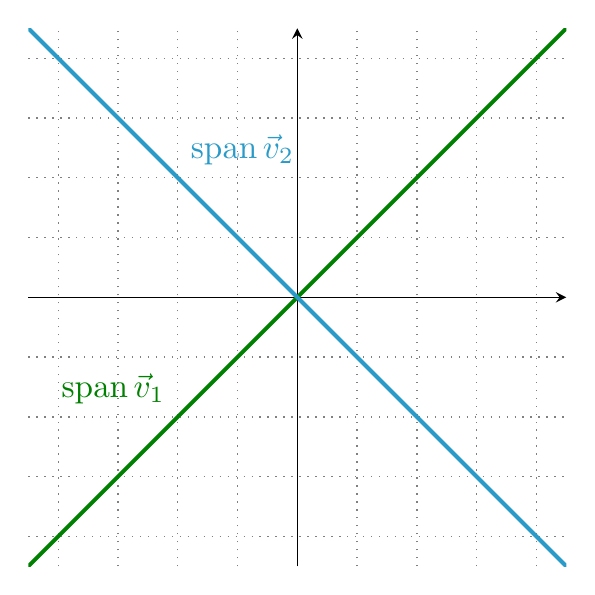
\begin{tikzpicture}[scale=1.2, >=latex]
			    \begin{axis}[scale=1,
					    axis equal image,
					    axis lines=middle,
					    axis line style = {black},
					    tick style={draw=none},
					    yticklabels={,,},
					    xticklabels={,,},
					 xmin=-4.5,
					 xmax=4.5,
					 ymin=-4.5,
					 ymax=4.5,
					 major grid style={dotted, gray},
					 xtick={-10,-9,...,10},
					 ytick={-10,-9,...,10},
					 grid=both,
					 anchor=origin]

				    \draw[Green, very thick] (-5,-5) -- (5,5) node[pos=.3, above left] {$\Span\Set{\vec v_1}$};
				    \draw[cyan!80!black, very thick] (-5,5) -- (5,-5) node[pos=.3, above right] {$\Span\Set{\vec v_2}$};
			    \end{axis}
				\end{tikzpicture}
			\end{solution}
		\item Describe $\Span\Set{\vec v_1,\vec v_2}$.
			\begin{solution}
				$\Span\Set{\vec v_1,\vec v_2} = \R^2$

				We can see this since for any $\mat{x\\y} \in \R^2$,
				\[
					\mat{x\\y}
					=\frac{x}{2}\left(\mat{1\\1}+\mat{1\\-1}\right)+\frac{y}{2}\left(\mat{1\\1}-\mat{1\\-1}\right)
					=\frac{x+y}{2}\vec v_1 + \frac{x-y}{2}\vec v_2
				\]
			\end{solution}
		\item Describe $\Span\Set{\vec v_1,\vec v_3}$.
			\begin{solution}[inline]
				$\Span\Set{\vec v_1,\vec v_3} = \Span\Set{\vec v_1}$,
				a line through the origin with direction vector $\vec v_1$.
			\end{solution}
		\item Describe $\Span\Set{\vec v_1,\vec v_2,\vec v_3}$.
			\begin{solution}[inline]
				$\Span\Set{\vec v_1,\vec v_2,\vec v_3} = \Span\Set{\vec v_1,\vec v_2} = \R^2$
			\end{solution}
	\end{parts}


\begin{lesson}
	\Title{Span, Translated Span}

	\Heading{Textbook}
	Section 1.2

	\Heading{Objectives}
	\begin{itemize}
		\item Explain why spans always go through the origin.
		\item Express lines or planes through the origin as spans.
		\item Express lines or planes not through the origin as translated spans.
	\end{itemize}

	\Heading{Motivation}
	Translated spans link vector form of lines and planes with sets and spans.
	Soon we will have the vocabulary of linear independence and be able to
	talk about independent direction vectors of a plane, but right now just connecting
	the concepts and notation is enough.

\end{lesson}

	\bookonlynewpage
	\question
	\begin{annotation}
		\begin{goals}
			\Goal{Connect geometric figures to spans.}

			The goal of this problem is to
			\begin{itemize}
				\item Identify a relationship between lines and spans.
				\item Describe a line through the origin as a span.
				\item Identify when a line cannot be described as a span.
				\item Apply the definition of $\Span X$ even when $X$ is infinite.
			\end{itemize}
		\end{goals}

		\begin{notes}
			\begin{itemize}
				\item The lines are not written in $y=mx+b$ form on purpose.
					We avoid this form in linear algebra since it cannot
					describe all lines.
				\item Part 3 will really stretch their minds. Students at this point are not used
					to applying definitions. They will have a conception of $\Span X$
					where $X$ is finite and will forget the definition because
					this conception is ``good enough''. This question forces
					them to think back to the definition.
			\end{itemize}
		\end{notes}
	\end{annotation}
	\label{linesAsSpans}
	Let $\ell_1\subseteq \R^2$ be the line with equation $x-y=0$ and $\ell_2\subseteq\R^2$
	the line with equation $x-y=4$.
	\begin{parts}
		\item If possible, describe $\ell_1$ as a span. Otherwise explain why
			it's not possible.
			\begin{solution}
				$\ell_1 = \Span\Set*{\mat{1\\1}}$, since $\mat{x\\y} \in \ell_1$
				if and only if $x = y$, which in turn is true if and only if it
				is a scalar multiple of $\mat{1\\1}$.
			\end{solution}
		\item If possible, describe $\ell_2$ as a span. Otherwise explain why it's
			not possible.
			\label{linesAsSpans.2}
			\begin{solution}
				This is not possible. $\mat{0\\0}$ is an element of	the span of
				\emph{any} set of vectors, since we can use all zeroes as the
				scalars in a linear combination, but $\mat{0\\0} \notin \ell_2$.
			\end{solution}
		\item Does the expression $\Span(\ell_1)$ make sense? If so, what is it?
			How about $\Span(\ell_2)$?
			\begin{solution}
				Both of these expressions do make sense. One can compute the span
				of any set of vectors, and these lines are just special set of
				points in $\R^2$ which we are already used to thinking of as vectors.

				$\Span(\ell_1) = \ell_1$, since all of the vectors on
				the line $\ell_1$ are already multiples of $\mat{1\\1}$, as we
				discovered earlier.

				$\Span(\ell_2)$ equals all of $\R^2$. It's easy to see that the
				vectors $v = \mat{4\\0}$ and $w = \mat{0\\-4}$ are both on $\ell_2$,
				and the span of these two vectors alone is all of $\R^2$.
			\end{solution}
	\end{parts}


	\bookonlynewpage
	\SavedDefinitionRender{SetAddition}


	\question
	\begin{annotation}
		\begin{goals}
			\Goal{Describing geometry using sets.}

			The goal of this problem is to
			\begin{itemize}
				\item Practice applying a new definition in a familiar context ($\R^2$).
				\item Gain an intuitive understanding of set addition.
				\item Describe lines that don't pass through $\vec 0$ using
					a combination of set addition and spans.
			\end{itemize}
		\end{goals}

		\begin{notes}
			\begin{itemize}
				\item Set addition will be brand new to most students, even
					those with a linear algebra background.
				\item Special care must be taken to differentiate
					$\vec a+\vec b$ and $\{\vec a\}+\{\vec b\}$.
				\item We will use set addition mainly as a mathematical
					notation to describe translated spans. In this
					case the summands will be an infinite set
					and a singleton. There is no need to explore the sum
					of two infinite sets.
			\end{itemize}
		\end{notes}
	\end{annotation}
	Let $A=\Set*{\mat{1\\2}}$, $B=\Set*{\mat{1\\1},\mat{1\\-1}}$,
	and $\ell=\Span\Set*{\mat{1\\-1}}$.
	\begin{parts}
		\item Draw $A$, $B$, and $A+B$ in the same picture.
			\begin{solution}
				\begin{tikzpicture}[scale=1.2, >=latex]
			    \begin{axis}[scale=1,
					    axis equal image,
					    axis line style={black},
					    axis lines=middle,
					    tick style={draw=none},
					    yticklabels={,,},
					    xticklabels={,,},
					 xmin=-4.5,
					 xmax=4.5,
					 ymin=-4.5,
					 ymax=4.5,
					 major grid style={dotted, gray},
					 xtick={-10,-9,...,10},
					 ytick={-10,-9,...,10},
					 grid=both,
					 anchor=origin]

				    %\draw[Green, very thick] (-5,0) -- (5,0) node[near end, below] {$H$};
				    %\draw[cyan!80!black, very thick] (0,-5) -- (0,5) node[near end, right] {$V$};
				    %\draw[orange!80!black, very thick] (-5,-5) -- (5,5) node[near end, below right] {$D$};


				    \fill[fill=Green] (1,2) circle[radius=2pt] node[left] {\color{Green}$A$};
				    \fill[fill=Red]
				    	(1,1) circle[radius=2pt]
				    	(1,-1) circle[radius=2pt] node[below right] {\color{Red}$B$}
				    ;
				    \fill[fill=Blue]
				    	(2,3) circle[radius=2pt]
				    	(2,1) circle[radius=2pt] node[below right] {\color{Blue}$A+B$}
				    ;
			    \end{axis}
			\end{tikzpicture}
			\end{solution}
		\item Is $A+B$ the same as $B+A$?
			\begin{solution}
				Yes. Since $A$ and $B$ are such small sets we could just
				compute all the vectors in $A+B$ and $B+A$ and see that they're
				equal. However, we know that real numbers can be added up in any
				order, and the coordinates of an element of $A+B$ or $B+A$ are
				simply sums of the corresponding coordinates of elements of $A$ and $B$.
			\end{solution}
		\item Draw $\ell+A$.
			\begin{solution}
				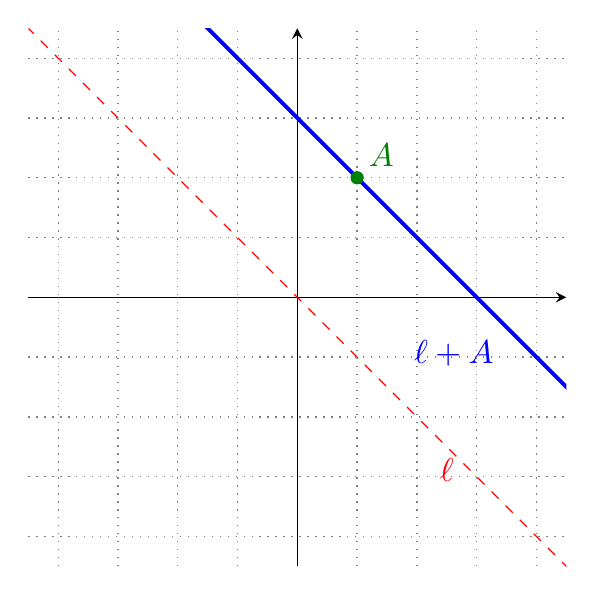
\begin{tikzpicture}[scale=1.2, >=latex]
			    \begin{axis}[scale=1,
					    axis equal image,
					    axis line style={black},
					    axis lines=middle,
					    tick style={draw=none},
					    yticklabels={,,},
					    xticklabels={,,},
					 xmin=-4.5,
					 xmax=4.5,
					 ymin=-4.5,
					 ymax=4.5,
					 major grid style={dotted, gray},
					 xtick={-10,-9,...,10},
					 ytick={-10,-9,...,10},
					 grid=both,
					 anchor=origin]

				    \draw[Red, thin, dashed] (-5,5) -- (5,-5) node[near end, below] {$\ell$};
				    \draw[Blue, very thick] (-4,7) -- (6,-3) node[near end, below left] {$\ell+A$};
				    \fill[fill=Green] (1,2) circle[radius=2pt] node[above right] {\color{Green}$A$};
			    \end{axis}
			\end{tikzpicture}
			\end{solution}
		\item Consider the line $\ell_2$ given in vector form by $\vec x=t\mat{1\\-1}+\mat{1\\2}$.
			Can $\ell_2$ be described using only a span? What about using a span
			and set addition?
			\begin{solution}
				$\ell_2$ cannot be described using only a span, for the same reason
				as the line $\ell_2$ in Problem \ref{linesAsSpans}.\ref{linesAsSpans.2}
				couldn't be. We know that the origin $\mat{0\\0}$ must be an element
				of any span, but it is not a point on $\ell_2$.

				$\ell_2$ can be described as a span plus a set addition though.
				Specifically, $\ell_2=\ell + A$.
			\end{solution}
	\end{parts}



\begin{lesson}
	\Title{Linear Independence \& Dependence}

	\Heading{Textbook}
	Section 1.2

	\Heading{Objectives}
	\begin{itemize}
		\item Define linear independence/dependence using spans.
		\item Pick linearly independent subsets with the same span by inspection.
		\item Explain why having a ``closed loop'' or trivial linear combination
			means a set is linearly dependent.
	\end{itemize}

	\Heading{Motivation}
	Linear independence/dependence is one of the biggest concepts in linear algebra.
	Linear independence/dependence tells us whether a set has redundant information
	in it with respect to spans. The idea of a having redundant information vs\mbox{.}
	not comes up all the time in the world (sometimes it's a plus, sometimes it's not).

	Knowing
	a set is independent tells us what its span will look like (in terms of what dimension
	it will be). It is also an abstract concept that has both a ``geometric'' definition
	and an ``algebraic'' one.
	\begin{annotation}
		\begin{notes}
			Don't define a linearly dependent \emph{set}, define
			a linearly dependent \emph{list}. Otherwise you cannot talk about
			$\mat{1\\1}$ and $\mat{1\\1}$ be linearly dependent since sets don't
			contain duplicates.
		\end{notes}
	\end{annotation}
	Geometrically, a set is linearly dependent if you can remove
	a vector without the span changing. Algebraically a set is linearly dependent if there
	is a non-trivial linear combination giving the zero vector. This lesson focuses on the
	geometric definition (with the algebraic definition coming next).

	Though the algebraic definition is easier to work with in proofs, the geometric definition
	provides intuition about how to visualize linearly
	dependent sets.

\end{lesson}

\begin{iola}
\section*{Task 1.3: The Magic Carpet, Getting Back Home}
\addcontentsline{toc}{subsection}{Task 1.3: The Magic Carpet Ride, Getting Back Home}

	\begin{annotation}
		\begin{goals}
			\Goal{Span in higher dimensions.}

			The goal of this problem is to
			\begin{itemize}
				\item Examine subtleties that exist in three dimensions that are
					missing in two dimensions.
				\item Apply linear algebra tools to answer open-ended questions.
			\end{itemize}
		\end{goals}

		\begin{notes}
			This problem is set up to prime
			theorems about linearly dependent vectors. In particular, it
			\begin{itemize}
				\item gives an example of a non-trivial linear combination giving $\vec 0$;
				\item shows that if there is one non-trivial linear combination giving $\vec 0$,
					there are others;
				\item shows that 3 non-parallel vectors in $\R^3$ need not span $\R^3$.
			\end{itemize}

			The problem also allows linking to previous linear algebra ideas. A system
			of equations can be used to find \emph{all} non-trivial solutions, and showing
			a particular system of equations is inconsistent will show that the span
			is not $\R^3$.
		\end{notes}
	\end{annotation}
Suppose you are now in a three-dimensional world for the carpet
ride problem, and you have three modes of transportation:
\[
	\vec v_1 = \mat{1 \\1 \\ 1}\qquad
	\vec v_2 = \mat{6 \\3 \\ 8}\qquad
	\vec v_3 = \mat{4 \\1 \\ 6}
\]

You are only allowed to use each mode of transportation \textbf{once}
(in the forward or backward direction) for a fixed amount of time ($c_1$
on $\vec v_1$, $c_2$ on $\vec v_2$, $c_3$ on $\vec v_3$).

\vspace{5mm}


\begin{enumerate}
	\item  Find the amounts of time on each mode of transportation ($c_1$, $c_2$,
		and $c_3$, respectively) needed to go on a journey that starts and ends
		at home \emph{or} explain why it is not possible to do so.

	\item Is there more than one way to make a journey that meets the
		requirements described above? (In other words, are there different
		combinations of times you can spend on the modes of transportation so
		that you can get back home?) If so, how?

	\item Is there anywhere in this 3D world that Gauss
		could hide from you? If so, where? If not, why not?

	\item What is $\Span\Set*{\mat{1\\1\\1},\mat{6\\3\\8},\mat{4\\1\\6}}$?

\end{enumerate}
\end{iola}


	\begin{annotation}
		\begin{goals}
			\Goal{Geometric definition of linear independence/dependence.}
		\end{goals}

		\begin{notes}
			\begin{itemize}
				\item This definition is conceptually simple but notationally hard.
				\item The definition is phrased in terms of a list of vectors (instead of
					a set) to avoid issues with the fact that sets cannot have repeated elements. (e.g.,
					if $\vec a\neq \vec 0$, then the set $\{\vec a,\vec a\}=\{\vec a\}$ is linearly
					independent, whereas the list of vectors $\vec a,\vec a$ is linearly dependent.)
				\item Many students will not realize that $\vec v_i$ is being ``left out''
					of the span.
				\item Students might assume, for example, that $\vec v_1$ could always be removed
					from the span. This misconception is targeted in a later problem.
				\item Have students rephrase this definition in plain language.
			\end{itemize}
		\end{notes}
	\end{annotation}

	\bookonlynewpage
	\SavedDefinitionRender{LinearlyDependentIndependentGeometric}

	\question
	\begin{annotation}
		\begin{goals}
			\Goal{Apply the (geometric) definition of linear independence/dependence.}

			The goal of this problem is to
			\begin{itemize}
				\item Develop a mental picture linking linear dependence and
					``redundant'' vectors.
				\item Practice applying a new definition.
				\item Find multiple linearly independent subsets of a linearly dependent set.
			\end{itemize}
		\end{goals}

		\begin{notes}
			\begin{itemize}
				\item Students won't find this problem hard.
				\item There may be some confusion about what ``describe'' means.
			\end{itemize}
		\end{notes}
	\end{annotation}
		Let $\vec u=\mat{1\\0\\0}$, $\vec v=\mat{0\\1\\0}$, and $\vec w=\mat{1\\1\\0}$.
	\begin{parts}
		\item Describe $\Span\Set{\vec u,\vec v,\vec w}$.
			\begin{solution}
				The $xy$-plane in $\R^3$. That is, the set of all vectors in $\R^3$ with $z$-coordinate
				equal to zero.
			\end{solution}
		\item Is $\{\vec u,\vec v,\vec w\}$ linearly independent? Why or why not?
			\begin{solution}
				No. $\vec w=\vec u+\vec v$, and so $\vec w \in \Span\Set{\vec u, \vec v}$.
			\end{solution}
	\end{parts}

	Let $X=\Set{\vec u,\vec v,\vec w}$.

	\begin{parts}[resume]
		\item Give a subset $Y\subseteq X$ so that $\Span Y=\Span X$ and $Y$ is
			linearly independent.
			\begin{solution}
				$Y = \Set{\vec u,\vec v}$ is one example that works.
			\end{solution}
		\item Give a subset $Z\subseteq X$ so that $\Span Z=\Span X$ and $Z$ is
			linearly independent and $Z\neq Y$.
			\begin{solution}
				$Z = \Set{\vec u, \vec w}$ and $Z = \Set{\vec v, \vec w}$ both have
				the same span as $Y$ above.
			\end{solution}
	\end{parts}


	\bookonlynewpage
	\SavedDefinitionRender{TrivialLinearCombination}

	\question
	\begin{annotation}
		\begin{goals}
			\Goal{Link trivial/non-trivial linear combinations to linear independence/dependence.}
		\end{goals}

		\begin{notes}
			\begin{itemize}
				\item Part 2 is a chance to practice writing arguments.
				\item Many students will mistakenly assume that non-trivial means
					\emph{all} coefficients are non-zero and use this in
					their argument. Bring out this misconception.
			\end{itemize}
		\end{notes}
	\end{annotation}
		Recall $\vec u=\mat{1\\0\\0}$, $\vec v=\mat{0\\1\\0}$, and $\vec w=\mat{1\\1\\0}$.
	\begin{parts}
		\item Consider the linearly dependent
			set $\Set{\vec u,\vec v,\vec w}$ (where $\vec u,\vec v,\vec w$ are
			defined as above). Can you write $\vec 0$ as a non-trivial linear
			combination of vectors in this set?
			\begin{solution}[inline]
				$\vec 0 = \vec u + \vec v - \vec w$.
			\end{solution}
		\item Consider the linearly independent set $\Set{\vec u,\vec v}$.
			Can you write $\vec 0$ as a non-trivial linear combination of
			vectors in this set?
			\begin{solution}
				No. Suppose
				\[
					a_1 \vec u + a_2 \vec v = \vec 0
				\]
				was a non-trivial linear combination. Then at least one of $a_1$ or $a_2$
				is non-zero. If $a_1$ is non-zero, then
				\[
					\vec u = -\frac{a_2}{a_1}\vec v
				\]
				and so $\vec u\in\Span\Set{\vec v}$.
				If $a_2$ is non-zero, then
				\[
					\vec v=-\frac{a_1}{a_2}\vec u.
				\]
				and so $\vec v\in\Span\Set{\vec u}$.
				In either case, $\{\vec u,\vec v\}$ would be linearly dependent.
			\end{solution}
	\end{parts}


\begin{lesson}
	\Title{Linear Independence \& Dependence---Equivalent Definitions}

	\Heading{Textbook}
	Section 1.2

	\Heading{Objectives}
	\begin{itemize}
		\item Define linear independence/dependence in terms of trivial linear combinations.
		\item Explain how the geometric and algebraic definitions of linear independence/dependence relate.
		\item Explain the connection between a vector equation having multiple
			solutions and those vectors being linearly independent/dependent.
		\item Identify the largest linearly independent set that could exist in $\R^n$.
	\end{itemize}

	\Heading{Motivation}
	We've done geometry, now let's do algebra. The geometric and algebraic definitions
	are equivalent, but they suggest different consequences. The geometric definition
	of linear independence tells us about the dimension of a span. The algebraic
	definition tells us about the number of solutions to a vector equation.

\end{lesson}

	We now have an equivalent definition of linear dependence.
	\begin{annotation}
		\begin{notes}
			\begin{itemize}
				\item The algebraic definition of linear independence/dependence
					is good for proofs but hard to intuit.
			\end{itemize}
		\end{notes}
	\end{annotation}

	\bookonlynewpage
	\SavedDefinitionRender{LinearlyDependentIndependentAlgebraic}

	\question
	\begin{annotation}
		\begin{goals}
			\Goal{Link algebraic and geometric definitions of linear independence/dependence.}

			The goal of this problem is to
			\begin{itemize}
				\item Understand how the algebraic and geometric definitions of linear
					independence/dependence relate.
				\item Practice writing mathematical arguments.
			\end{itemize}
		\end{goals}

		\begin{notes}
			\begin{itemize}
				\item You could easily spend an entire class working with students
					to get well-written proofs. Be mindful of time. Since
					this is not a proofs-based course, we want to focus on the intuition here.
			\end{itemize}
		\end{notes}
	\end{annotation}
	\begin{parts}
		\item Explain how this algebraic definition (new) implies the geometric one (original).
			\begin{solution}
				Suppose the vectors $\vec v_1, \vec v_2, \dots, \vec v_n$ is
				linearly dependent in this new sense. That means there are
				scalars	$a_1, a_2, \dots, a_n$, at least one of which is non-zero,
				such that
				\[
					a_1 \vec v_1 + \cdots + a_n \vec v_n = 0.
				\]
				Suppose $a_i\neq 0$. Then
				\[
					\vec v_i = \tfrac{-a_1}{a_i}\vec v_1+\cdots +\tfrac{-a_{i-1}}{a_i}\vec v_{i-1}
					+\tfrac{-a_{i+1}}{a_i}\vec v_{i+1}+\cdots+\tfrac{-a_n}{a_i}\vec v_n.
				\]
				This means $\vec v_i\in \Span\Set{\vec v_1,\ldots,\vec v_{i-1},\vec v_{i+1},\ldots,\vec v_n}$,
				which is precisely the geometric definition of linear dependence.
			\end{solution}
		\item Explain how the geometric definition (original) implies this algebraic one (new).
			\begin{solution}
				Suppose that $\vec v_1, \vec v_2, \dots, \vec v_n$ are linearly
				dependent according to the geometric definition. Fix $i$ so that
				$\vec v_i\in \Span\Set{\vec v_1,\ldots,\vec v_{i-1},\vec v_{i+1},\ldots,\vec v_n}$.

				By the definition of $\Span$, we know that
				\[
					\vec v_i=\beta_1\vec v_1+\cdots +\beta_{i-1}\vec v_{i-1}+\beta_{i+1}\vec v_{i+1}
					+\cdots +\beta_n\vec v_{n}.
				\]
				Thus
				\[
					\vec 0 = -\vec v_i+\beta_1\vec v_1+\cdots +\beta_{i-1}\vec v_{i-1}+\beta_{i+1}\vec v_{i+1}
					+\cdots +\beta_n\vec v_{n},
				\]
				and this is a non-trivial linear combination since the coefficient of $\vec v_i$ is $-1\neq 0$.
			\end{solution}
	\end{parts}

	Since we have geometric def $\implies$ algebraic def, and algebraic def $\implies$ geometric def
	($\implies$ should be read aloud as `implies'), the two definitions
	are \emph{equivalent} (which we write as algebraic def $\iff$ geometric def).


	\bookonlynewpage
	\question
	\begin{annotation}
		\begin{goals}
			\Goal{Linear dependence and infinite solutions.}

			The goal of this problem is to
			\begin{itemize}
				\item Connect linear dependence with infinite solutions.
				\item Connect linear independence with unique solutions.
			\end{itemize}
		\end{goals}

		\begin{notes}
			\begin{itemize}
				\item Part 1 won't give the students much trouble.
				\item Part 2 will be hard. The idea that you could add $\vec 0$
					but change the coefficients of a linear combination
					is hard to thin of and even harder to write correctly.
			\end{itemize}
		\end{notes}
	\end{annotation}
	Suppose for some unknown $\vec u, \vec v, \vec w$, and $\vec a$,
	\[
		\vec a = 3\vec u+2\vec v +\vec w\qquad \text{and}\qquad
		\vec a = 2\vec u+\vec v -\vec w.
	\]
	\begin{parts}
		\item Could the set $\Set{\vec u,\vec v,\vec w}$ be linearly
		independent?
			\begin{solution}
				No. If both equations are true, they would combine to show
				\[
					3\vec u+2\vec v +\vec w = 2\vec u+\vec v -\vec w.
				\]
				Collecting all the terms on the left side, we get:
				\[
					\vec u + \vec v + 2\vec w = \vec 0,
				\]
				which is a non-trivial linear combination of vectors in the given
				set equalling the zero vector.
			\end{solution}
	\end{parts}
	Suppose that
	\[
		\vec a = \vec u+6\vec r-\vec s
	\]
	is the \emph{only} way to write $\vec a$ using $\vec u,\vec r,\vec s$.
	\begin{parts}[resume]
		\item Is $\Set{\vec u,\vec r,\vec s}$ linearly independent?
			\begin{solution}
				Yes. If it were not, there would exist scalars $a_1, a_2, a_3$,
				not all of which are zero, such that:
				\[
					a_1 \vec u + a_2 \vec r + a_3\vec s = \vec 0.
				\]
				But then
				\[
					\vec u+6\vec r-\vec s + (a_1 \vec u + a_2 \vec r + a_3\vec s)
				\]
				would be another way to write $\vec a$ using only the same three
				vectors.
			\end{solution}
		\item Is $\Set{\vec u,\vec r}$ linearly independent?
			\begin{solution}
				Yes. If it were not, we would necessarily have $\vec u = \beta \vec r$
				for some scalar $\beta$. But then
				\[
					(\beta + 6) \vec r - \vec s
				\]
				would be another way to write $\vec a$ using only the same three
				vectors.
			\end{solution}
		\item Is $\Set{\vec u,\vec v,\vec w,\vec r}$ linearly independent?
			\begin{solution}
				No. We know from earlier that $\vec u+\vec v+2\vec w=\vec 0$, and
				so $\vec u+\vec v+2\vec w+0\vec r=\vec 0$ is a non-trivial linear
				combination of the vectors in this set that equals the zero vector.
			\end{solution}
	\end{parts}


\begin{iola}
\section*{Task 1.4: Linear Independence and Dependence, Creating Examples}
\addcontentsline{toc}{subsection}{Task 1.4: Linear Independence and Dependence, Creating Examples}



\begin{enumerate}
	\item Fill in the following chart keeping track of the strategies you used to generate
examples.

\vspace{2mm}

\begin{center}
\begin{tabular}{|c|c|c|}
	\hline
	&Linearly independent & Linearly dependent \\
	\hline
	A set of 2 vectors in $\R^2$ &&\\
	\hline
	A set of 3 vectors in $\R^2$ &&\\
	\hline
	A set of 2 vectors in $\R^3$ &&\\
	\hline
	A set of 3 vectors in $\R^3$ &&\\
	\hline
	A set of 4 vectors in $\R^3$ &&\\
	\hline
\end{tabular}
\end{center}

		\item Write at least two generalizations that can
			be made from these examples and the strategies you
			used to create them.
	\begin{annotation}
		\begin{notes}
			\begin{itemize}
				\item Make sure ``more than $n$ vectors in $\R^n$
					is linearly dependent'' comes out.
			\end{itemize}
		\end{notes}
	\end{annotation}

\end{enumerate}

\end{iola}


\begin{module}
	\Title{Dot Products \& Normal Forms}

	In this module you will learn
	\begin{itemize}
		\item Geometric an algebraic definitions of the dot product.
		\item How dot products relate to the length of a vector and the angle
			between two vectors.
		\item The \emph{normal form} of lines, planes, and hyperplanes.
	\end{itemize}

	Let $\vec a$ and $\vec b$ be vectors rooted at the same point and let
$\theta$ denote the \emph{smaller} of the
two angles between them, so $0\leq \theta \leq \pi$.
The \emph{dot product}\index{dot product} of $\vec a$ and $\vec b$ is defined to be
\[
	\vec a\cdot \vec b=\norm{\vec a}\norm{\vec b}\cos \theta.
\]
We will call this the \emph{geometric definition of the dot product}.
The dot product is also sometimes called the \emph{scalar product} because
the result is a scalar.
Note that $\vec a\cdot\vec b = 0$ when either $\vec a$ or $\vec b$ is zero or,
more interestingly, if their directions are perpendicular.

\begin{center}
	\newcommand{\tikzAngleOfLine}{\tikz@AngleOfLine}
	  \def\tikz@AngleOfLine(#1)(#2)#3{%
	  \pgfmathanglebetweenpoints{%
	    \pgfpointanchor{#1}{center}}{%
	    \pgfpointanchor{#2}{center}}
	  \pgfmathsetmacro{#3}{\pgfmathresult}%
	  }
	\newcommand{\tikzMarkAngle}[3]{
	\tikzAngleOfLine#1#2{\AngleStart}
	\tikzAngleOfLine#1#3{\AngleEnd}
	\draw #1+(\AngleStart:0.35cm) arc (\AngleStart:\AngleEnd:0.35cm);
	}
	\usetikzlibrary{patterns,decorations.pathreplacing}
	\begin{tikzpicture}
		\coordinate (A) at (2,1);
		\coordinate (B) at (.5,2);
		\coordinate (O) at (0,0);

		\draw[->,thick,myred!60!white] (0,0) -- +(A) node [midway,below right] {$\vec a$};
		\draw[->,thick,mypink] (0,0) -- +(B) node [midway,above left] {$\vec b$};
		\tikzMarkAngle{(O)}{(A)}{(B)}
		\node at ($(O)+(50:.65)$) {$\theta$};
	\end{tikzpicture}
	\hspace{1cm}
	\begin{tikzpicture}
		\coordinate (A) at (-2,-1);
		\coordinate (B) at (.5,2);
		\coordinate (O) at (0,0);

		\draw[->,thick,myred!60!white] (0,0) -- +(A) node [midway,below right] {$\vec a$};
		\draw[->,thick,mypink] (0,0) -- +(B) node [midway,above left] {$\vec b$};
		\tikzMarkAngle{(O)}{(B)}{(A)}
		\node at ($(O)+(140:.65)$) {$\theta$};
	\end{tikzpicture}
\end{center}

Algebraically, we can define the dot product in terms of coordinates:
\[
	\matc{a_1\\a_2\\\vdots\\a_n}\cdot \matc{b_1\\b_2\\\vdots\\b_n}
	=a_1b_1+a_2b_2+\cdots+a_nb_n.
\]
We will call this the \emph{algebraic definition of the dot product}.

By switching between algebraic and geometric definitions, we can use the dot
product to find quantities that are otherwise difficult to find.
\begin{example}
	Find the angle between the vectors $\vec v=(1,2,3)$ and $\vec w=(1,1,-2)$.

	From the algebraic definition of the dot product, we know
	\[
		\vec v\cdot \vec w = 1(1)+2(1)+3(-2) = -3.
	\]
	From the geometric definition, we know
	\[
		\vec v\cdot \vec w=\norm{\vec v}\norm{\vec w}\cos\theta
		=\sqrt{14}\sqrt{6}\cos\theta=2\sqrt{21}\cos\theta.
	\]
	Equating the two definitions of $\vec v\cdot \vec w$, we see
	\[
		\cos\theta = \frac{-3}{2\sqrt{21}}
	\]
	and so $\theta=\arccos\Big(\tfrac{-3}{2\sqrt{21}}\Big)$.
\end{example}

The dot product has several interesting properties. Since the angle between
$\vec a$ and itself is $0$, the geometric definition of the dot product tells us
\[
	\vec a\cdot \vec a=\Norm{\vec a}\Norm{\vec a}\cos 0 = \Norm{\vec a}^2.
\]
In other words,
\[
	\Norm{\vec a}=\sqrt{\vec a\cdot \vec a},
\]
and so dot products can be used to compute the length of vectors\footnote{ Oftentimes in
non-geometric settings, the dot product between two vectors is defined first and then
the length of $\vec a$ is actually \emph{defined} to be $\sqrt{\vec a\cdot \vec a}$.}.

From the algebraic definition of the dot product, we can deduce several distributive laws.
Namely, for any vectors $\vec a$, $\vec b$, and $\vec c$ and any scalar $k$ we have
\[
	(\vec a+\vec b)\cdot\vec c = \vec a\cdot \vec c+\vec b\cdot \vec c\qquad
	\vec a\cdot(\vec b+\vec c)=\vec a\cdot \vec b+\vec a\cdot \vec c
\]
\[
	(k\vec a)\cdot \vec b = k(\vec a\cdot \vec b)=\vec a\cdot (k\vec b)
\]
and
\[
	\vec a\cdot \vec b=\vec b\cdot \vec a.
\]

\Heading{Orthogonality}
Recall that for vectors $\vec a$ and $\vec b$, the relationship $\vec a\cdot \vec b=0$
can hold for two reasons: (i) either $\vec a=\vec 0$, $\vec b=\vec 0$, or both
or (ii) $\vec a$ and $\vec b$ meet at $90^{\circ}$.  Thus, the dot product
can be used to tell if two vectors are perpendicular.  There is some strangeness
with the zero vector here, but it turns out this strangeness simplifies our lives
mathematically.

\SavedDefinitionRender{Orthogonal}

The definition of orthogonal encapsulates both the idea of two vectors forming
a right angle and the idea of one of them being $\vec 0$.

Before we continue, let's pin down the idea of one vector pointing
in the \emph{direction}\index{direction}\index{positive direction} of another.  
There are many ways we could define
this idea, but we'll go with this one.

\SavedDefinitionRender{Direction}

The vector $2\xhat$ points in the direction of $\xhat$ since
$\frac{1}{2}(2\xhat)=\xhat$.  Since $\frac{1}{2}>0$, $2\xhat$ also points
in the positive direction of $\xhat$. In contrast, 
$-\xhat$ points in the direction $\xhat$ but not the positive direction of $\xhat$.

When it comes to the relationship between two vectors, there are two extremes: they
point in the same direction, or they are orthogonal. The dot product can be used to
tell you which of these cases you're in, and more than that, it can tell you to 
what extent one vector points in the direction of another (even if they don't point in
the same direction).

\begin{example}
	Let $\vec a=\mat{1\\2}$, $\vec b=\mat{3\\3}$, $\vec c=\mat{2\\1}$, and $\vec v=\mat{3\\4}$. Which vector out of
	$\vec a$, $\vec b$, and $\vec c$ has a direction closest to the direction of $\vec v$?

	XXX Finish
\end{example}


\Heading{Normal Form of Lines and Planes}

Let $\vec n=\mat{1\\2}$. If a vector $\vec v=\mat{v_1\\v_2}$ is orthogonal to $\vec n$, then
\[
	\vec n\cdot\vec v=v_1+2v_2=0,
\]
and so $v_1=-2v_2$. In other words, $\vec v$ is orthogonal to $\vec n$ exactly when $\vec v\in\Span\Set*{\mat{-2\\1}}$.
What have we learned? The set of all vectors orthogonal to $\vec n$ forms a line $\ell=\Span\Set*{\mat{-2\\1}}$. In
this case, we call $\vec n$ a \emph{normal vector} for $\ell$.

\begin{center}
	\begin{tikzpicture}
		\def\dotMarkRightAngle[size=#1](#2,#3,#4){%
		 \draw ($(#3)!#1!(#2)$) -- 
		       ($($(#3)!#1!(#2)$)!#1!90:(#2)$) --
		       ($(#3)!#1!(#4)$);
		 \path (#3) -- ($($(#3)!#1!(#2)$)!#1!90:(#2)$);
		}
		\begin{axis}[
		    anchor=origin,
		    name=plot1,
		    disabledatascaling,
		    xmin=-3,xmax=3,
		    ymin=-2,ymax=2,
			xtick={-4,...,4},
			ytick={-2,...,4},
		    x=1cm,y=1cm,
		    grid=both,
		    grid style={line width=.1pt, draw=gray!10},
		    %major grid style={line width=.2pt,draw=gray!50},
		    axis lines=middle,
		    minor tick num=0,
		    enlargelimits={abs=0.5},
		    axis line style={latex-latex},
		    ticklabel style={font=\tiny,fill=white},
		    xlabel style={at={(ticklabel* cs:1)},anchor=north west},
		    ylabel style={at={(ticklabel* cs:1)},anchor=south west}
		]
			\coordinate (A) at (1,2);
			\coordinate (O) at (0,0);
			\coordinate (B) at (2,-1);
			\dotMarkRightAngle[size=6pt](B,O,A);
			\draw[mypink, thick] ($-2*(-2,1)$) -- ($2*(-2,1)$);
			\draw[mygreen, thick, ->] (0,0) -- (1,2) node[midway, below right] {$\vec n$};
		\end{axis}
		\node[mypink, above right] at (2,-1.2) {$\ell=\Span\Set*{\mat{-2\\1}}$};
	\end{tikzpicture}
\end{center}

\SavedDefinitionRender{NormalVector}

In $\R^2$, normal vectors provide yet another way to describe lines, including lines which don't pass
through the origin.

Let $n=\mat{1\\2}$ as before, and fix $\vec p=\mat{1\\1}$. If we draw the set of all vectors
orthogonal to $\vec n$ but \emph{root all the vectors at $\vec p$}, again we get a line, but this
time the line passes through $\vec p$.

\begin{center}
	\begin{tikzpicture}
		\def\dotMarkRightAngle[size=#1](#2,#3,#4){%
		 \draw ($(#3)!#1!(#2)$) -- 
		       ($($(#3)!#1!(#2)$)!#1!90:(#2)$) --
		       ($(#3)!#1!(#4)$);
		 \path (#3) -- ($($(#3)!#1!(#2)$)!#1!90:(#2)$);
		}
		\begin{axis}[
		    anchor=origin,
		    name=plot1,
		    disabledatascaling,
		    xmin=-2,xmax=4,
		    ymin=-1,ymax=3,
			xtick={-4,...,4},
			ytick={-2,...,4},
		    x=1cm,y=1cm,
		    grid=both,
		    grid style={line width=.1pt, draw=gray!10},
		    %major grid style={line width=.2pt,draw=gray!50},
		    axis lines=middle,
		    minor tick num=0,
		    enlargelimits={abs=0.5},
		    axis line style={latex-latex},
		    ticklabel style={font=\tiny,fill=white},
		    xlabel style={at={(ticklabel* cs:1)},anchor=north west},
		    ylabel style={at={(ticklabel* cs:1)},anchor=south west}
		]
			\begin{scope}[cm={1,0,0,1,(1,1)}]
				\coordinate (A) at (1,2);
				\coordinate (O) at (0,0);
				\coordinate (B) at (2,-1);
				\dotMarkRightAngle[size=6pt](B,O,A);
				\draw[mypink, thick] ($-2*(-2,1)$) -- ($2*(-2,1)$);
				\draw[mygreen, thick, ->] (0,0) -- (1,2) node[midway, below right] {$\vec n$};
				\fill[myorange] (0,0) node[below left] {$\vec p$} circle (2pt);
			\end{scope}
		\end{axis}
		\node[mypink, above right] at (3,0) {$\ell_2=\Span\Set*{\mat{-2\\1}}+\Set*{\mat{1\\1}}$};
	\end{tikzpicture}
\end{center}

In fact, the line we get is $\ell_2=\Span\Set*{\mat{-2\\1}}+\Set*{\mat{1\\1}}=\ell+\Set{\vec p}$, which is just $\ell$ (the
parallel line through the origin) translated by $\vec p$. 

Let's relate this to dot products and normal vectors. By definition, for every $\vec v\in \ell$, we have $\vec n\cdot \vec v=0$.
Since $\ell_2$ is a translate of $\ell$ by $\vec p$, we deduce the relationship that for every $\vec v\in \ell_2$,
\[
	\vec n\cdot(\vec v-\vec p) = 0,
\]
and this is the \emph{normal form} of a line in $\R^2$.

\SavedDefinitionRender{NormalFormofaLine}


\bigskip
What about in $\R^3$? 
Fix a non-zero vector $\vec n\in\R^3$ and let $\mathcal Q\subseteq\R^3$ be the set of vectors orthogonal to $\vec n$.
$\mathcal Q$ is a plane through the origin, and again, we call $\vec n$ a \emph{normal vector}\index{normal vector} of the plane $\mathcal Q$.


\begin{center}
\begin{tikzpicture}
	\newcommand{\RightAngle}[4][5pt]{%
        \draw ($#3!#1!#2$)
        --($ #3!2!($($#3!#1!#2$)!.5!($#3!#1!#4$)$) $)
        --($#3!#1!#4$) ;
        }
    \begin{axis}[grid=major,view={20}{40},z buffer=sort,
	    width=12cm,
	    scale mode=scale uniformly,
	    zmin=-5,zmax=5,xmin=-10,xmax=10,ymin=-10,ymax=10,
	    xticklabels={,,}, yticklabels={,,}, zticklabels={,,},
	    xtick={-10,-5,...,10}, ytick={-10,-5,...,10}
	    ]
		\addplot3 [data cs=cart,surf,domain=-10:10,samples=2, opacity=0.5]
		{.25*x+.25*y};
		\coordinate (A) at (axis cs:-4,-4,-2);
		\coordinate (N) at (axis cs:-6,-6,6);
		\coordinate (B) at (axis cs:4,4,2);
		\coordinate (C) at (axis cs:-4,4,0);

		\draw [mypink,fill] (A) circle (1.5pt) node [below right] {$\vec 0$};
		\draw [->, thick] (A) -- (B) node [midway,below right] {$\vec d_1$};
		\draw [->, thick] (A) -- (C) node [midway,above left] {$\vec d_2$};
		\draw [->, thick] (A) -- (N) node [midway,left] {$\vec n$};
		\RightAngle{(N)}{(A)}{(C)}
		%\RightAngle{(N)}{(A)}{(B)}
    \end{axis}
  \end{tikzpicture}
\end{center}

In a similar way to the case of a line, $\mathcal Q$ is the set of solutions to $\vec n\cdot \vec x=0$.
And, for any $\vec p\in\R^3$, the translated plane $\mathcal Q+\Set{\vec p}$ is the solution set to
\[
	\vec n\cdot (\vec x-\vec p)=0.
\]
Thus, we see planes in $\R^3$ have a normal form just like lines in $\R^2$ do. 

\begin{example}
	Find vector form and normal form of the plane $\mathcal P$ passing
	through the point $A=(1,0,0)$, $B=(0,1,0)$ and $C=(0,0,1)$.

	To find vector form of $\mathcal P$, we need a point on the plane and
	two direction vectors.  We have three points on the plane, so we can
	obtain two direction vectors by subtracting these points in different ways.
	Let
	\[
		\vec d_1=\overrightarrow{AB} = \mat{-1\\1\\0}\qquad\vec d_2=\overrightarrow{AC}=
		\mat{-1\\0\\1}.
	\]
	Using the point $A$, we may now write vector form of $\mathcal P$ as
	\[
		\mat{x\\y\\z} = t\mat{-1\\1\\0}+s\mat{-1\\0\\1}+\mat{1\\0\\0}.
	\]

	To write normal form we need to find a normal vector to $\mathcal P$.  By inspection,
	we can see that $\vec n=(1,1,1)$ is a normal vector to $\mathcal P$.  If we weren't
	so insightful, we could also solve the system $\vec n\cdot \vec d_1=0$ and $\vec n\cdot\vec d_2=0$ to find a
	normal vector.  Now, we may express $\mathcal P$ in normal form as
	\[
		\mat{1\\1\\1}\cdot\left(\mat{x\\y\\z}-\mat{1\\0\\0}\right)=0.
	\]
\end{example}

In $\R^2$, only lines have a normal form, and in $\R^3$ only planes have a normal form. In general,
we call objects in $\R^n$ which have a normal form \emph{hyperplanes}.

\SavedDefinitionRender{Hyperplane}

Hyperplanes always have dimension one less than the space they're contained in. So, hyperplanes in
$\R^2$ are (one-dimensional) lines, hyperplanes in $\R^3$ are regular (two-dimensional) planes, 
and hyperplanes in $\R^4$ are (three-dimensional) volumes.

\Heading{Hyperplanes and Linear Equations}

Suppose $\vec n,\vec p\in \R^3$ and $\vec n\neq \vec 0$. Then, solutions to 
\[
		\vec n\cdot(\vec x-\vec p)=0
\]
define a plane $\mathcal P$. But, $\vec n\cdot (\vec x-\vec p)=0$
if and only if
\[
		\vec n\cdot\vec x = \vec n\cdot \vec p = \alpha.
\]
Since $\vec n$ and $\vec p$ are fixed, $\alpha$ is a constant. Expanding using
coordinates, we see
\[
		\vec n\cdot(\vec x-\vec p)=\vec n\cdot\vec x-\alpha=
		n_xx+n_yy+n_zz-\alpha=0
\]
and so $\mathcal P$ is the set of solutions to
\begin{equation}
	\label{EQScalarForm}
		n_xx+n_yy+n_zz=\alpha.
\end{equation}
Equation \eqref{EQScalarForm} is sometimes
called \emph{scalar form}\index{scalar form of a plane}
of a plane.  For us, it will not be important to distinguish between scalar and normal form, but
what is important is that we can use the row reduction algorithm to write the complete solution
to \eqref{EQScalarForm}, and this complete solution will necessarily be written in vector form.

\begin{example}
	Let $\mathcal Q\subseteq \R^3$ be the plane passing through $\vec p$ and with normal vector $\vec n$ where
	\[
		\vec p=\mat{1\\1\\0}\qquad\text{and}\qquad\vec n=\mat{1\\1\\1}.
	\]
	Write $\mathcal Q$ in vector form.

	We know $\mathcal Q$ is the set of solutions to $\vec n\cdot (\vec x-\vec p)=0$. In scalar form, this equation
	becomes
	\[
		\vec n\cdot (\vec x-\vec p)=\vec n\cdot \vec x-\vec n\cdot \vec p = x+y+z-2=0.
	\]
	Rearranging, we see $\mathcal Q$ is the set of all solutions to
	\[
		x+y+z=2.
	\]
	Using the row reduction algorithm to write the complete solution\footnote{ In some sense, this is overkill
	because the equation corresponds to the augmented matrix $\mat{1&1&1&\!\!\!\!|\!\!\!\!&2}$, which is already row reduced.}, we get
	\[
		\mat{x\\y\\z}=t\mat{-1\\1\\0}+s\mat{-1\\0\\1}+\mat{2\\0\\0}.
	\]
\end{example}



\end{module}

\begin{lesson}
	\Title{Dot Product, Orthogonality}

	\Heading{Textbook}
	Section 1.3

	\Heading{Objectives}
	\begin{itemize}
		\item Compute the dot product of two vectors.
		\item Compute the length of a vector.
		\item Find the distance between two vectors.
		\item Define what it means for vectors to be orthogonal.
		\item Interpret the sign of the dot product geometrically.
		\item Create a unit vector in the direction of another.
	\end{itemize}

	\Heading{Motivation}
	Studying $\R^n$ we're in a natural inner product space with lengths and
	angles. The dot product allows us to get at lengths and angles. It will
	also give an alternative way to compute matrix products (dot product with rows
	instead of linear combination of columns).

	Most importantly, the dot product tells us how much two vectors point in
	the same direction as well as when they're orthogonal.

\end{lesson}


	\bookonlynewpage
\section*{Dot Product}
	\begin{annotation}
		\begin{notes}
			\begin{itemize}
				\item It'd be great to say $\norm{\vec v}=\sqrt{\vec v\cdot \vec v}$,
					but that would make the geometric definition of the dot product circular.
			\end{itemize}
		\end{notes}
	\end{annotation}

	\SavedDefinitionRender{Norm}

	\begin{annotation}
		\begin{notes}
			\begin{itemize}
				\item The two definitions are useful in different contexts.
				\item Students will gravitate towards the algebraic definition because
					it has an easier formula. Emphasize that if they don't know
					both definitions, there will be problems they can't solve.
			\end{itemize}
		\end{notes}
	\end{annotation}

	\SavedDefinitionRender{DotProduct}

	\question
	\begin{annotation}
		\begin{goals}
			\Goal{Practicing dot products.}

			The goal of this problem is to
			\begin{itemize}
				\item Use both the algebraic and geometric definitions of the dot product
					as appropriate to compute dot products.
				\item Gain an intuition that positive dot product
					means ``pointing in similar directions'', negative dot product
					means ``pointing in opposite directions'', and zero dot product
					means ``pointing in orthogonal directions''.
			\end{itemize}
		\end{goals}

		\begin{notes}
			\begin{itemize}
				\item For part 3(d), some students will suggest a vector
					that ``points out of the page''. This is a great idea!
					Except that such a vector would have the wrong number of components,
					so the dot products wouldn't be defined.
				\item For part 4, students will try to solve an equation. Encourage them
					to guess-and-check instead. It will be much faster.
			\end{itemize}
		\end{notes}
	\end{annotation}

		Let $\vec a=\mat{1\\1}$, $\vec b=\mat{3\\1}$, and $\vec u=\mat{1\\2\\1}$.
	\begin{parts}
		\item
		\begin{enumerate}
			\item Draw a picture of $\vec a $ and $\vec b$.
				\begin{solution}
				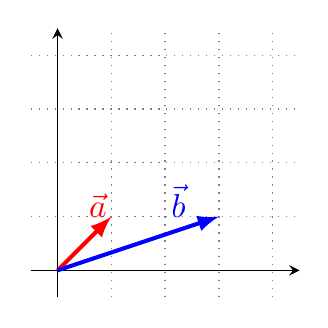
\begin{tikzpicture}[scale=1.2, >=latex]
			    \begin{axis}[scale=.5,
					    axis equal image,
					    axis line style={black},
					    axis lines=middle,
					    tick style={draw=none},
					    yticklabels={,,},
					    xticklabels={,,},
					 xmin=-.5,
					 xmax=4.5,
					 ymin=-.5,
					 ymax=4.5,
					 major grid style={dotted, gray},
					 xtick={-10,-9,...,10},
					 ytick={-10,-9,...,10},
					 grid=both,
					 anchor=origin]

				    \draw[Red, very thick, ->] (0,0) -- (1,1) node[near end, above] {$\vec a$};
				    \draw[Blue, very thick, ->] (0,0) -- (3,1) node[near end, above] {$\vec b$};
			    \end{axis}
			\end{tikzpicture}
				\end{solution}
			\item Compute $\vec a\cdot \vec b$.
				\begin{solution}[inline]
					$\vec a\cdot \vec b = (1)(3) + (1)(1) = 4$.
				\end{solution}
			\item Find $\|\vec a\|$ and $\|\vec b\|$ and use your knowledge of
			the multiple ways to compute the dot product to find $\theta$,
			the angle between $\vec a$ and $\vec b$. Label $\theta$ on your picture.
				\begin{solution}
					$\|\vec a\| = \sqrt{(1)^2 + (1)^2} = \sqrt{2}$ and
					$\|\vec b\| = \sqrt{(3)^2 + (1)^2} = \sqrt{10}$.

					Using the two definitions of the dot product we have:
					\begin{align*}
						\vec a\cdot \vec b &= \|\vec a\|\|\vec b\|\cos \theta \\
						\implies 4 &= (\sqrt{2})(\sqrt{10}) \cos \theta \\
						\implies \theta &= \arccos\left( \frac{2}{\sqrt{5}}\right)
					\end{align*}
				\end{solution}
		\end{enumerate}
		\item Draw the graph of $\cos$ and identify which angles make $\cos$
			negative, zero,	or positive.
			\begin{solution}
				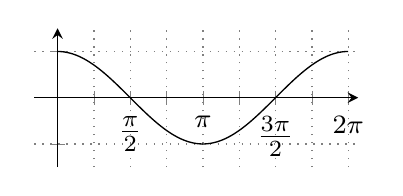
\begin{tikzpicture}[scale=1.2, >=latex]
			    \begin{axis}[scale=.5,
					    axis equal image,
					    axis line style={black},
					    axis lines=middle,
					    yticklabels={,,},
					    xticklabels={,,},
					 xmin=-.5,
					 xmax=6.5,
					 ymin=-1.5,
					 ymax=1.5,
					 major grid style={dotted, gray},
					 xtick={0,.7854,...,6.284},
					 xticklabels={,,$\tfrac{\pi}{2}$,,\footnotesize $\pi$,,$\tfrac{3\pi}{2}$,,\footnotesize $2\pi$},
					 ytick={-10,-9,...,10},
					 grid=both,
					 anchor=origin]

					 \addplot[domain=0:6.283,samples=100] {cos(180/3.1415*x)};
			    \end{axis}
				\end{tikzpicture}

				Cosine is positive for angles in the interval $\left(-\frac{\pi}{2},\frac{\pi}{2}\right)$,
				as well as all shifts of this interval by a multiple of $2\pi$ in
				either direction.

				$\cos$ is positive for angles in the interval $\left(\frac{\pi}{2},\frac{3\pi}{2}\right)$,
				as well as all shifts of this interval by a multiple of $2\pi$ in
				either direction.
			\end{solution}

		\item Draw a new picture of $\vec a$ and $\vec b$ and on that picture draw
		\begin{enumerate}
			\item a vector $\vec c$ where $\vec c\cdot \vec a$ is negative.
			\item a vector $\vec d$ where $\vec d\cdot \vec a=0$ and $\vec d\cdot \vec b < 0$.
			\item a vector $\vec e$ where $\vec e\cdot \vec a=0$ and $\vec e\cdot \vec b>0$.
			\item Could you find a vector $\vec f$ where $\vec f\cdot \vec a=0$ and $\vec f\cdot \vec b=0$?
				Explain why or why not.
				\begin{solution}
				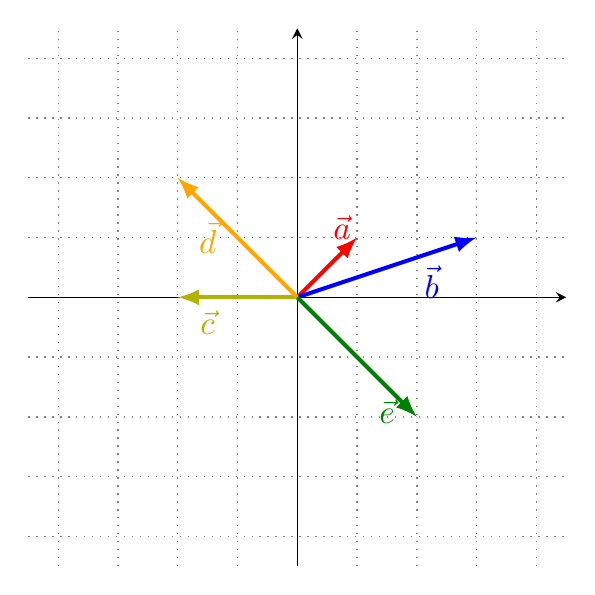
\begin{tikzpicture}[scale=1.2, >=latex]
			    \begin{axis}[scale=1,
					    axis equal image,
					    axis line style={black},
					    axis lines=middle,
					    tick style={draw=none},
					    yticklabels={,,},
					    xticklabels={,,},
					 xmin=-4.5,
					 xmax=4.5,
					 ymin=-4.5,
					 ymax=4.5,
					 major grid style={dotted, gray},
					 xtick={-10,-9,...,10},
					 ytick={-10,-9,...,10},
					 grid=both,
					 anchor=origin]

				    \draw[Red, very thick, ->] (0,0) -- (1,1) node[near end, above] {$\vec a$};
				    \draw[Blue, very thick, ->] (0,0) -- (3,1) node[near end, below] {$\vec b$};
				    \draw[Yellow!70!black, very thick, ->] (0,0) -- (-2,0) node[near end, below] {$\vec c$};
				    \draw[Orange, very thick, ->] (0,0) -- (-2,2) node[near end, below] {$\vec d$};
				    \draw[Green, very thick, ->] (0,0) -- (2,-2) node[near end, below] {$\vec e$};
			    \end{axis}
			\end{tikzpicture}

					(d) $\vec f = \vec 0$ is the only possibility. For any vector
					$\vec f = \mat{x\\y}$, we can compute:
					\[
						\vec f\cdot \vec a = x + y
						\qquad \text{and} \qquad
						\vec f\cdot \vec b = 3x + y.
					\]
					If these both equal zero, the first equation says that $y = -x$,
					and in turn the second one says $x = 0$ (and so $y = 0$ as well).
				\end{solution}
		\end{enumerate}

		\item Recall the vector $\vec u$ whose coordinates are given at the beginning of this problem.
		\begin{enumerate}
			\item Write down a vector $\vec v$ so that the angle between $\vec u$
				and $\vec v$ is $\pi/2$. (Hint, how does this relate to the dot
				product?)
				\begin{solution}
					$\vec v = \mat{1\\1\\-3}$ is one such vector.

					Since $\cos(\pi/2) = 0$, from the second definition of the dot
					product above we know we are looking for a $\vec v$ such that
					$\vec u \cdot \vec v = 0$. Using the first definition of the
					dot product, we can see that the $\vec v$ given above is one
					possibility.
				\end{solution}
			\item Write down another vector $\vec w$ (in a different direction from
				$\vec v$) so that the angle between $\vec w$ and $\vec u$ is $\pi/2$.
				\begin{solution}
					$\vec w = \mat{-1\\1\\-1}$ is a possible answer.

					$\vec u \cdot \vec w = 0$, and $\vec w$ is clearly not parallel
					to $\vec v$ from above.
				\end{solution}
			\item Can you write down other vectors different than both $\vec v$
				and $\vec w$ that still	form an angle of $\pi/2$ with $\vec u$?
				How many such vectors are there?
				\begin{solution}
					Yes. $\mat{0\\2\\-4}$ is one possibility.

					There are actually infinitely many such vectors; any linear
					combination of $\vec w$ and $\vec v$ will work.

					To see this, note that any such vector $\vec x$ is of the form
					\[
						\vec x = t \mat{1\\1\\-3} + s \mat{-1\\1\\-1}
						= \matc{t-s\\t+s\\-3t-s},
					\]
					for scalars $t$ and $s$. We can then compute
					\[
						\vec u \cdot \vec x = (1)(t-s) + (2)(t+s) + (1)(-3t-s) = 0,
					\]
					and so any such vector $\vec x$ forms an angle of $\pi/2$
					with $\vec u$.
				\end{solution}
		\end{enumerate}
	\end{parts}

	\bookonlynewpage
	\displayonlynewpage
	\begin{theorem}
		For a vector $\vec v\in \R^n$, the formula
		\[
			\|\vec v\| = \sqrt{\vec v\cdot \vec v}
		\]
		always holds.
	\end{theorem}

	\SavedDefinitionRender{Distance}

	\SavedDefinitionRender{UnitVector}

	\question
	\begin{annotation}
		\begin{goals}
			\Goal{Practice using norms.}

			The goal of this problem is to
			\begin{itemize}
				\item Practice finding the distance between two vectors.
				\item Produce a unit vector pointing in the same direction as another vector.
				\item Intuitively apply the triangle inequality: $\norm{\vec a+\vec b}\leq \norm{\vec a}+\norm{\vec b}$.
			\end{itemize}
		\end{goals}

		\begin{notes}
			\begin{itemize}
				\item Part 1 will be easy.
				\item Many will have trouble with part 2. Encourage them to write definitions! $\vec a$ is
					in the direction of $\vec u$ if $\vec a=k\vec u$ and $\vec a$ is a unit vector if $\norm{\vec a}=1$.
					Now, solve for $k$.

					They will forget that $\sqrt{k^2}=\abs{k}$ and so there are two solutions
					unless you insist on $k\geq 0$. You could mention ``in the direction of'' vs. the
					more specific ``in the positive direction of'' if you want to have a detailed discussion.
				\item Have them draw a picture for part 3.
				\item Part 4 will be very hard. Only go into it if you have plenty of time.
			\end{itemize}
		\end{notes}
	\end{annotation}
	Let $\vec u=\mat{1\\2\\1}$ and $\vec v=\mat{1\\1\\3}$.
	\begin{parts}
		\item Find the distance between $\vec u$ and $\vec v$.
			\begin{solution}
				$\vec u - \vec v = \mat{0\\1\\-2}$, and so $\norm{\vec u-\vec v} = \sqrt{5}$.
			\end{solution}
		\item Find a unit vector in the direction of $\vec u$.
			\begin{solution}
				$\frac{1}{\sqrt{6}} \vec u = \mat{\frac{1}{\sqrt{6}}\\\frac{2}{\sqrt{6}}\\\frac{1}{\sqrt{6}}}$.

				$\norm{\vec u} = \sqrt{6}$, and so if we multiply $\vec u$ by $\frac{1}{\sqrt{6}}$,
				the length of the resulting vector will be 1.
			\end{solution}
		\item Does there exist a \emph{unit vector} $\vec x$ that is distance
			$1$ from $\vec u$?
			\begin{solution}
				No. $\norm{\vec u} = \sqrt{6}$, and so the shortest length that a
				vector whose distance from $\vec u$ is 1 can have is $\sqrt{6} - 1$,
				which is greater than 1.
			\end{solution}
		\item Suppose $\vec y$ is a unit vector and the distance between $\vec y$
			and	$\vec u$ is $2$. What is the angle between $\vec y$ and $\vec u$?
			\begin{solution}
				The angle between $\vec u$ and $\vec y$ is $\arccos\left(\frac{3}{2\sqrt{6}}\right)$.

				By assumption, $2=\norm{\vec u-\vec y}$, and so
				\begin{align*}
					4 &= \norm{\vec u-\vec y}^2\\
					&= (\vec u-\vec y)\cdot(\vec u-\vec y)\\
					&= \vec u\cdot\vec u - 2(\vec u\cdot\vec y) + \vec y\cdot\vec y\\
					&=\norm{\vec u}^2 - 2\vec u\cdot\vec y + \norm{\vec y}^2\\
					&=6 - 2\vec u\cdot\vec y + 1.
				\end{align*}
				Then we rearrange to find that $\vec u\cdot \vec y = \frac{3}{2}$.

				Using this in the second definition of the dot product, we see:
				\[
					\frac{3}{2} = \left(\sqrt{6}\right)(1) \cos \theta,
				\]
				where $\theta$ is the angle between $\vec u$ and $\vec y$.
			\end{solution}
	\end{parts}

	\bookonlynewpage
	\SavedDefinitionRender{Orthogonal}

	\question
	\begin{annotation}
		\begin{goals}
			\Goal{Apply the definition of \emph{orthogonal}.}

			The goal of this problem is to
			\begin{itemize}
				\item Gain an intuitive understanding of \emph{orthogonal vectors}.
				\item Produce orthogonal vectors via guess-and-check.
				\item Apply the Pythagorean theorem to orthogonal vectors to find lengths.
			\end{itemize}
		\end{goals}

		\begin{notes}
			\begin{itemize}
				\item It won't occur to most students that $\vec 0$ is orthogonal to everything. Make sure
					this come up.
				\item Guessing-and-checking is a valid and useful mathematical technique. Student aren't
					comfortable with this method because there's no algorithm for it (and so it
					doesn't seem reliable and repeatable). We should change their attitude. Most problems
					in their lives won't be solved with repeatable algorithms (unless they work on
					an assembly line).
			\end{itemize}
		\end{notes}
	\end{annotation}
	\begin{parts}
		\item Find two vectors orthogonal to $\vec a=\mat{1\\-3}$.  Can you find
			two such vectors that are not parallel?
			\begin{solution}
				Two such vectors are $\mat{3\\1}$ and $\mat{-6\\-2}$.

				It is impossible for two non-parallel vectors to both be
				orthogonal to $\vec a$. If $\vec b = \mat{x\\y}$ is orthogonal to
				$\vec a$, then we must have that $x - 3y = 0$, or in other words
				that $x = 3y$. Any $\vec b$ satisfying this is a multiple of
				$\mat{3\\1}$.
			\end{solution}
		\item Find two vectors orthogonal to $\vec b=\mat{1\\-3\\4}$.  Can you
			find two such vectors that are not parallel?
			\begin{solution}
				Two such vectors are $\mat{7\\1\\-1}$ and $\mat{2\\2\\1}$.

				These two vectors are not parallel.
			\end{solution}
		\item Suppose $\vec x$ and $\vec y$ are orthogonal to each other and
			$\norm{\vec x}=5$ and $\norm{\vec y}=3$. What is the distance between
			$\vec x$ and $\vec y$?
			\begin{solution}
				The distance between them must be $\sqrt{34}$.

				One way to see this is with Pythagoras' theorem. Two perpendicular
				line segments of lengths 3 and 5 form the two shorter sides of a
				right angle triangle, and so the length of the third side is
				$\sqrt{5^2 + 3^2} = \sqrt{34}$.

				An equivalent way to see this is to use what we know about dot
				products to calculate $\norm{\vec x-\vec y}$ as follows:
				\[
					\norm{\vec x-\vec y} = \sqrt{(\vec x-\vec y)\cdot(\vec x-\vec y)}
					= \sqrt{\norm{\vec x}^2 - 2(\vec x\cdot\vec y) + \norm{\vec y}^2}
					= \sqrt{5^2 + 2(0) + 3^2},
				\]
				where in the last step we've used the fact that $\vec x$ and $\vec y$
				are orthogonal, so $\vec x\cdot\vec y = 0$.
			\end{solution}
	\end{parts}

\begin{lesson}
	\Title{Normal Form of Lines and Planes}

	\Heading{Textbook}
	Section 1.3

	\Heading{Objectives}
	\begin{itemize}
		\item Describe lines and planes in normal form.
	\end{itemize}

	\Heading{Motivation}
	Physics often describes surfaces in terms of normal and tangential components.
	Normal form of lines and planes is one way to get at this decomposition. Further, thinking
	about lines and planes in terms of right angles will help when visualizing orthogonal projections.

\end{lesson}

	\bookonlynewpage
	\question
	\begin{annotation}
		\begin{goals}
			\Goal{Generate lines using orthogonality.}

			The goal of this problem is to
			\begin{itemize}
				\item Visually see how the set of all vectors orthogonal to
					a given vector forms a line.
				\item Given a line defined as the set of all vectors orthogonal
					to a given vector, express the line using an equation or
					span.
			\end{itemize}
		\end{goals}

		\begin{notes}
			\begin{itemize}
				\item This problem won't be hard, so don't spend too much time on it.
				\item For part 1, students might insist on drawing arrowheads and tails
					on their vectors. This is an opportunity to discuss when you should
					draw arrowheads/tails and when you shouldn't.
			\end{itemize}
		\end{notes}
	\end{annotation}
	\begin{parts}
		\item Draw $\vec u=\mat{2\\3}$ and \emph{all} vectors orthogonal to it.
			Call this set $A$.
			\begin{solution}
				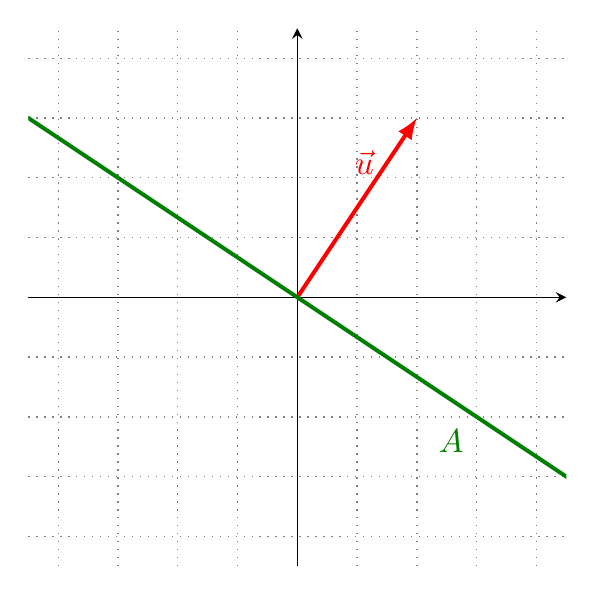
\begin{tikzpicture}[scale=1.2, >=latex]
			    \begin{axis}[scale=1,
					    axis equal image,
					    axis line style={black},
					    axis lines=middle,
					    tick style={draw=none},
					    yticklabels={,,},
					    xticklabels={,,},
					 xmin=-4.5,
					 xmax=4.5,
					 ymin=-4.5,
					 ymax=4.5,
					 major grid style={dotted, gray},
					 xtick={-10,-9,...,10},
					 ytick={-10,-9,...,10},
					 grid=both,
					 anchor=origin]

				    \draw[Red, very thick, ->] (0,0) -- (2,3) node[near end, left] {$\vec u$};
				    \draw[Green, very thick] (-6,4) -- (6,-4) node[near end, below left] {$A$};
			    \end{axis}
			\end{tikzpicture}
			\end{solution}
		\item If $\vec x=\mat{x\\y}$ and $\vec x$ is orthogonal to $\vec u$,
			what is $\vec x\cdot \vec u$?
			\begin{solution}[inline]
				$\vec x\cdot \vec u = 0$, by the definition of orthogonality.
			\end{solution}
		\item Expand the dot product $\vec u\cdot \vec x$ to get an equation for $A$.
			\begin{solution}
				$A$ is the line with vector equation $\vec x = t\mat{3\\-2}$.

				If $\vec x=\mat{x\\y} \in A$, then $\vec x\cdot\vec u = 2x + 3y = 0$.
			\end{solution}
		\item If possible, express $A$ as a span.
			\begin{solution}[inline]
				$A = \Span\Set*{\mat{3\\-2}}$.
			\end{solution}
	\end{parts}

	\bookonlynewpage
	\displayonlynewpage
	\SavedDefinitionRender{NormalVector}

	\question
	\begin{annotation}
		\begin{goals}
			\Goal{Express lines in normal form.}

			The goal of this problem is to
			\begin{itemize}
				\item Express lines, including lines that don't pass through $\vec 0$,
					in normal form.
				\item See the $\vec q$ in $\vec n\cdot (\vec x-\vec q)=0$ is similar
					to the $\vec p$ in the vector form $\vec x=t\vec d+\vec p$ in
					that it accommodates lines that don't pass through $\vec 0$.
				\item Use the dot product to represent a line compactly.
			\end{itemize}
		\end{goals}

		\begin{notes}
			\begin{itemize}
				\item In part 2 there may be some lingering confusion about the difference between
					a vector and a point. In particular, $\vec u-\vec p$ is a direction vector for $\ell_2$,
					but is not \emph{contained in} $\ell_2$.
				\item In part 3, have a discussion about the role that $\vec q$ plays. Namely,
					that it ``translates'', in a similar way that $\vec p$ in the vector
					form $\vec x=t\vec d+\vec p$ translates.

					However, be careful about the discussion here. Students may find it very
					confusing that we ``subtract $\vec q$'' to translate in normal form, whereas in
					vector form we add $\vec p$. Have a good explanation prepared if you go
					down this route.
			\end{itemize}
		\end{notes}
	\end{annotation}
	Let $\vec d=\mat{1\\2}$ and $\vec p=\mat{1\\-1}$, and define the lines
	\[
		\ell_1 = \Span\Set{\vec d}\qquad\text{and}\qquad \ell_2=\Span\Set{\vec d}+\Set{\vec p}.
	\]
	\begin{parts}
		\item Find a vector $\vec n$ that is a normal vector for both $\ell_1$
			and	$\ell_2$.
			\begin{solution}
				$\vec n=\mat{2\\-1}$ is one possibility.

				This vector is orthogonal to $\vec d$, which is a direction
				vector for both lines.
			\end{solution}
		\item Let $\vec v\in \ell_1$ and $\vec u\in \ell_2$.
			What is $\vec n\cdot \vec v$? What about $\vec n\cdot (\vec u-\vec p)$? Explain using a picture.
			\begin{solution}
				$\vec n\cdot \vec v =\vec n\cdot(\vec u-\vec p)= 0$.
				
				This is because any $\vec v \in \ell_1$ is a multiple
				of $\vec d$, which is orthogonal to $\vec n$. Similarly, for any $\vec u\in \ell_2$,
				the vector $\vec u-\vec p$ is a direction vector for $\ell_2$, and so it is orthogonal to $\vec n$.

				$\vec n\cdot \vec u=3$, since any such $\vec u$ is of the form
				$\vec u=\vec p+t\vec d$ for some scalar $t$, and so
				\[
					\vec n\cdot \vec u
					=\vec n\cdot (\vec p+t\vec d)
					=\vec n\cdot \vec p+t(\vec n\cdot \vec d)
					=3+t(0)
					=3.
				\]
			\end{solution}
		\item A line is expressed in \emph{normal form} if it is represented by
			an equation of the form $\vec n\cdot (\vec x-\vec q)=0$ for some
			$\vec n$ and $\vec q$. Express $\ell_1$ and $\ell_2$ in normal form.
			\begin{solution}
				A normal form of $\ell_1$ is $\mat{2\\-1}\cdot\vec x=0$.

				A normal form of $\ell_2$ is $\mat{2\\-1}\cdot\left(\vec x-\mat{1\\-1}\right)=0$.
				In the previous part we saw that $\vec n\cdot \vec x=\vec n\cdot \vec p$
				for all $\vec x\in \ell_2$, or in other words $\vec n\cdot (\vec x-\vec p) = 0$.
			\end{solution}
		\item Some textbooks would claim that $\ell_2$ could be expressed in normal form as {\color{cyan}$\mat{2\\-1}\cdot \vec x=3$}.
			How does this relate to the $\vec n\cdot(\vec x-\vec p)=0$ normal form? Where does the $3$ come from?
			\begin{solution}
				Let $\vec n=\mat{2\\-1}$ and let $\vec x\in \ell_2$. From the previous part, we know
				\[
					0=\vec n\cdot (\vec x-\vec p)
					=\vec n\cdot \vec x-\vec n\cdot \vec p
					=\vec n\cdot \vec x-3.
				\]
				Therefore
				\[
					\vec n\cdot \vec x= 3.
				\]
			\end{solution}
	\end{parts}

	\bookonlynewpage
	\question
	\begin{annotation}
		\begin{goals}
			\Goal{Planes in normal form.}

			The goal of this problem is to
			\begin{itemize}
				\item Observe that the set of all vectors orthogonal to another in $\R^3$
					is a plane.
				\item Translate descriptions of sets into precise mathematical statements using
					set-builder notation.
				\item Express a plane in multiple ways.
			\end{itemize}
		\end{goals}

		\begin{notes}
			\begin{itemize}
				\item Students have already worked with this plane in problem \ref{ProbPlane},
					but they won't remember. Emphasize part 1 and go quickly through the other parts,
					referring to problem \ref{ProbPlane} if needed.
			\end{itemize}
		\end{notes}
	\end{annotation}
	Let $\vec n=\mat{1\\1\\1}$.
	\begin{parts}
		\item Use set-builder notation to write down the set, $X$, of
			all vectors orthogonal to $\vec n$. Describe this set
			geometrically.
			\begin{solution}
				$X = \Set*{\vec x\in \R^3 \given \vec x\cdot \vec n = 0}$.

				Geometrically, this is a plane through the origin and
				perpendicular to $\vec n$.
			\end{solution}
		\item Describe $X$ using an equation.
			\begin{solution}[inline]
				$x+y+z=0$.
			\end{solution}
		\item Describe $X$ as a span.
			\begin{solution}[inline]
				$X = \Span\Set*{\mat{1\\-1\\0},\mat{1\\0\\-1}}$ is one way to do this.
			\end{solution}
	\end{parts}


\begin{module}
	\Title{Projections \& Vector Components}

	In this module you will learn
	\begin{itemize}
		\item The definition of the projection of a vector and the vector component of one vector
			in the direction of another.
		\item The relationship between projection, orthogonality, and vector components.
		\item How to project a vector onto a line.
	\end{itemize}

	\input{modules/module5.tex}

\end{module}
\begin{lesson}
	\Title{Projections}

	\Heading{Textbook}
	Section 1.4

	\Heading{Objectives}
	\begin{itemize}
		\item Project a vector onto lines and finite sets.
		\item Find the vector components of one vector in terms of another.
	\end{itemize}

	\Heading{Motivation}
	Projection of a vector onto a set, defined as the closet point in the
	set to the vector, is a general operation used outside of linear algebra.
	However, in the land of linear algebra, we have exact formulas for the
	projection of a vector onto particular sets (e.g., subspaces). 
	Projections are a chance to explore a seemingly simple definition
	and see it relate to sets, lines, normal form, and vector form.

	\begin{annotation}
		\begin{notes}
			In this class, we don't write $\Proj_{\vec v}\vec u$,
			i.e., the projection of one vector onto another. We
			instead call this $\Comp_{\vec v}\vec u$. We do this so
			as not to confuse $\Proj_{\{\vec v\}}\vec u$ and
			$\Comp_{\vec v}\vec u$. One is projection onto a singleton.
			The other is $\frac{\vec u\cdot \vec v}{\vec v\cdot \vec v}\vec v$.
		\end{notes}
	\end{annotation}
	$\Comp_{\vec v}\vec u$ is the vector component of a vector in the direction of another,
	which is sometimes called the ``projection'' of $\vec u$ onto $\vec v$ (but we're not using
	this terminology!). It relates
	to how much one vector points in the direction of another and
	provides a decomposition of vectors in terms of orthogonal components.


\end{lesson}
	\bookonlynewpage
\section*{Projections}

	\SavedDefinitionRender{Projection}

	\question
	\begin{annotation}
		\begin{goals}
			\Goal{Apply the definition of projection.}

			The goal of this problem is to
			\begin{itemize}
				\item Use the definition of projection to compute projections onto finite sets and lines.
				\item Pick an appropriate representation of a line to solve a projection problem.
			\end{itemize}
		\end{goals}
		\begin{notes}
			\begin{itemize}
				\item Projections will be new and strange. Some students will be familiar with
					the notation $\Proj_{\vec b}\vec a$ and will confuse this
					with $\Proj_{\{\vec b\}}\vec a$. Make them apply the definition of projection.
				\item When visualizing projections, it is often better to draw vectors as dots instead
					of line segments. Students will have a cluttered diagram if they try to
					draw vectors with ``tails''.
				\item General projections have no formula. This might make students unhappy, but it's an
					important point to emphasize.
				\item The goal of part 3 is to have students pick a from the many representations of $\ell$
					a suitable one. Vector avoids multivariable calculus.

				\item Some students might already know about a relationship between orthogonality and
					a closest point. If you don't want to optimize a quadratic,
					you may ask students to do part 4 first with a picture and then do part 3 by inspection.
			\end{itemize}
		\end{notes}
	\end{annotation}
	Let $\vec a=\mat{1\\0}$, $\vec b=\mat{4\\0}$, $\vec v=\mat{2\\2}$ and
	$\ell=\Span\Set{\vec a}$.
	\begin{parts}
		\item Draw $\vec a$, $\vec b$, and $\vec v$ in the same picture.
			\begin{solution}
				\begin{tikzpicture}[scale=1.2, >=latex]
			    \begin{axis}[scale=1,
					    axis equal image,
					    axis line style={black},
					    axis lines=middle,
					    tick style={draw=none},
					    yticklabels={,,},
					    xticklabels={,,},
					 xmin=-4.5,
					 xmax=4.5,
					 ymin=-4.5,
					 ymax=4.5,
					 major grid style={dotted, gray},
					 xtick={-10,-9,...,10},
					 ytick={-10,-9,...,10},
					 grid=both,
					 anchor=origin]

				    \fill[fill=Red] (1,0) circle[radius=2pt] node[below right] {\color{Red}$\vec a$};
				    \fill[fill=Green] (4,0) circle[radius=2pt] node[below right] {\color{Green}$\vec b$};
				    \fill[fill=Orange] (2,2) circle[radius=2pt] node[below right] {\color{Orange}$\vec v$};
			    \end{axis}
			\end{tikzpicture}
			\end{solution}
		\item Find $\Proj_{\Set{\vec b}}\vec v$, $\Proj_{\Set{\vec a,\vec b}}\vec v$.
			\begin{solution}
				$\Proj_{\Set{\vec b}}\vec v = \vec b$. Since there is only one
				point in $\Set{\vec b}$, it must be the closest point to $\vec v$.

				$\Proj_{\Set{\vec a,\vec b}}\vec v=\vec a$. We can simply compute
				$\norm{\vec v-\vec a} = \sqrt{5}$ and $\norm{\vec v-\vec b} = \sqrt{8}$,
				so $\vec a$ is closer to $\vec v$.
			\end{solution}
		\item Find $\Proj_\ell \vec v$. (Recall that a quadratic $at^2+bt+c$ has
			a minimum at $t=-\tfrac{b}{2a}$).
			\begin{solution}
				$\Proj_\ell \vec v = 2\vec a=\mat{2\\0}$.

				Any point in $\ell$ is of the form $t\vec a$ for some scalar
				$t$. The distance between such a point and $\vec v$ is
				\[
					\norm{\vec v - t\vec a}
					=\sqrt{\norm{v}^2 - 2t(\vec v\cdot \vec a) + t^2 \norm{a}^2}
					=\sqrt{8 - 4t + t^2}
				\]
				The quadratic inside the square root has a minimum at
				$t = 2$, so $2 \vec a$ is the closest point in the line
				to $\vec v$.
			\end{solution}
		\item Is $\vec v-\Proj_\ell \vec v$ a normal vector for $\ell$?
			Why or why not?
			\begin{solution}
				Yes.

				By the previous part, $\vec v-\Proj_\ell \vec v=\vec v-2\vec a=\mat{0\\2}$.
				This vector is orthogonal to $\vec a$, and therefore to $\ell$.
			\end{solution}
	\end{parts}

	\bookonlynewpage
	\question
	\begin{annotation}
		\begin{goals}
			\Goal{Project onto lines.}

			The goal of this problem is to
			\begin{itemize}
				\item Use orthogonality to compute the projection onto a line.
				\item Project onto lines that don't pass through $\vec 0$.
			\end{itemize}
		\end{goals}

		\begin{notes}
			\begin{itemize}
				\item This is not a calculus class, so we want to avoid
					doing projections via calculus. This problem forces
					the use of orthogonality to solve a projection question.
				\item When drawing pictures for part 2, there will be a question
					of where you should root your vectors. Rooting your vectors
					on $K$ makes the picture clearer.
			\end{itemize}
		\end{notes}
	\end{annotation}
	Let $K$ be the line given in vector form by $\vec x=t\mat{1\\2}+\mat{1\\0}$ and let
	$\vec c=\mat{1\\3}$.
	\begin{parts}
		\item Make a sketch with $\vec c$, $K$, and $\Proj_K\vec c$ (you don't need to compute
		$\Proj_K\vec c$ exactly).
			\begin{solution}
				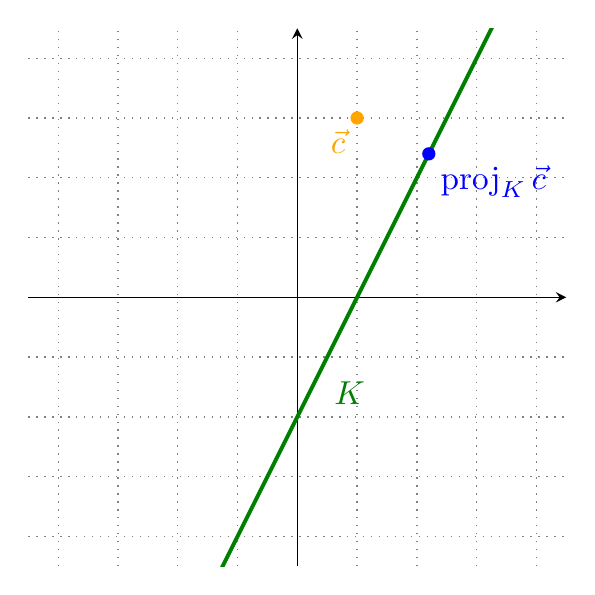
\begin{tikzpicture}[scale=1.2, >=latex]
			    \begin{axis}[scale=1,
					    axis equal image,
					    axis line style={black},
					    axis lines=middle,
					    tick style={draw=none},
					    yticklabels={,,},
					    xticklabels={,,},
					 xmin=-4.5,
					 xmax=4.5,
					 ymin=-4.5,
					 ymax=4.5,
					 major grid style={dotted, gray},
					 xtick={-10,-9,...,10},
					 ytick={-10,-9,...,10},
					 grid=both,
					 anchor=origin]

				    \draw[Green, very thick] (-2,-6) -- (4,6) node[pos=.4, below right] {$K$};

				    \fill[fill=Orange] (1,3) circle[radius=2pt] node[below left] {\color{Orange}$\vec c$};
				    \fill[fill=blue] (.2*11,.2*12) circle[radius=2pt] node[below right] {\color{blue}$\Proj_K\vec c$};
			    \end{axis}
			\end{tikzpicture}
			\end{solution}
		\item What should $(\vec c-\Proj_K\vec c)\cdot \mat{1\\2}$ be? Explain.
			\begin{solution}
				$(\vec c-\Proj_K\vec c)\cdot \mat{1\\2} = 0$.

				From our picture we can see that $c-\Proj_K\vec c$ is perpendicular
				to the line $K$, and so the dot product of this vector with any
				direction vector for $K$ should be zero.
			\end{solution}
		\item Use your formula from the previous part to find $\Proj_K\vec c$
			\emph{without} computing any distances.
			\begin{solution}
				$\Proj_K\vec c = \frac{1}{5}\mat{11\\12}$

				If $\Proj_K\vec c = \mat{x\\y}$, the formula from the previous
				part tells us
				\[
					\left(\mat{1\\3}-\mat{x\\y}\right)\cdot \mat{1\\2}
					=1-x+6-2y=0
					\quad \iff \quad
					x+2y=7
				\]
				So we need a point on $K$ that satisfies this equation. In other
				words, we need
				\[
					(t+1) + 2(2t) = 7 \quad \implies \quad t = \frac{6}{5}.
				\]
				The point on $K$ for this value of $t$ is $\frac{1}{5}\mat{11\\12}$.
			\end{solution}
	\end{parts}

	\bookonlynewpage
	\SavedDefinitionRender{Component}

	\begin{annotation}
		\begin{notes}
			\begin{itemize}
				\item This is called $\Proj_{\vec v}\vec u$ in some courses. This
					operation is renamed \emph{component \ldots} to avoid
					possible notational confusion with $\Proj_{\Set{\vec v}}\vec u$.
			\end{itemize}
		\end{notes}
	\end{annotation}

	\question
	\begin{annotation}
		\begin{goals}
			\Goal{Component of a vector in the direction of another.}

			The goal of this problem is to
			\begin{itemize}
				\item Read and apply a new definition.
				\item Use orthogonality to obtain a formula for components in terms of
					dot products.
			\end{itemize}
		\end{goals}

		\begin{notes}
			\begin{itemize}
				\item For part 1, ask students to codify their conditions
					with formulas. This will be \emph{hard}. Students
					will not know how to read the definition, They will
					get one property easily, but a second property will escape them.
				\item Part 2 is an exercise in applying the two formulas from part 1.
			\end{itemize}
		\end{notes}
	\end{annotation}
	Let $\vec a,\vec b\in \R^3$ be unknown vectors.
	\begin{parts}
		\item List two conditions that $\Comp_{\vec b}\vec a$ must satisfy.
			\begin{solution}
				$\Comp_{\vec b} \vec a$ must be a scalar multiple of $\vec b$.

				$\vec a - \Comp_{\vec b} \vec a$ must be orthogonal to $\vec b$,
				or in other words $(\vec a-\Comp_{\vec b}\vec a)\cdot \vec b=0$.
			\end{solution}
		\item Find a formula for $\Comp_{\vec b}\vec a$.
			\begin{solution}
				$\Comp_{\vec b}\vec a = \dfrac{\vec a\cdot\vec b}{\vec b\cdot\vec b} \vec b$.

				From the previous part, we should have $\Comp_{\vec b}\vec a=t\vec b$
				for some scalar $t$, and $(\vec a-\Comp_{\vec b}\vec a)\cdot \vec b=0$.

				Combining these, we get:
				\[
					0=(\vec a-t \vec b)\cdot \vec b
					=\vec a\cdot\vec b - t\vec b\cdot\vec b
					=\vec a\cdot\vec b - t(\vec b\cdot\vec b).
				\]
				Solving for $t$, we get $t = \dfrac{\vec a\cdot\vec b}{\vec b\cdot\vec b}$.
			\end{solution}
	\end{parts}


\begin{lesson}
	\Title{Projections, Subspaces}

	\Heading{Textbook}
	Sections 1.2, 1.4

	\Heading{Objectives}
	\begin{itemize}
		\item Identify $\Proj_{\Span\{\vec v\}}\vec u$ with $\Comp_{\vec v}\vec u$.
		\item Identify $\Comp_{\vec v}\vec u$ and $\Comp_{\alpha\vec v}\vec u$
			for all $\alpha\neq 0$, including negative $\alpha$.
		\item Define subspace.
		\item Distinguish subspaces and non-subspaces of $\R^2$.
	\end{itemize}

	\Heading{Motivation}
	Spans are a constructive way to describe lines, planes, and other
	flat objects. Subspaces are a categorical way of defining flat objects.
	Instead of explaining how to find the vectors in a set, we list their
	properties. This is a really powerful idea that facilitates abstraction.

	\begin{annotation}
		\begin{notes}
			\begin{itemize}
			\item	Philosophically, a subspace should be defined
			as a non-empty set closed under linear combinations.
			However, defining it as closed under addition and scalar
			multiplication gives students new to proofs
			something explicit to hang on to when attempting a proof.
			\item Some people define a subspace as a set containing
			$\vec 0$ and satisfying closure. We define a subspace
			as a non-empty set satisfying closure. We won't be trying
			to trick students by asking if an empty set is a subspace,
			so don't belabor the point.
			\item Proving a set is a subspace is one of the few proofs
				that we will hold students accountable for. That is,
					it is one of the few things we expect
					students to be able to write down completely
					correctly using formal mathematical language.
					They will need practice to be able to do this!
			\end{itemize}
		\end{notes}
	\end{annotation}
	Since we do not do abstract vector spaces in this course, subspaces are
	the first place (unless you count projections) students will encounter
	a set defined by its properties. Subspaces are suitable for a first-encounter
	because 1) the properties are simple and familiar and 2) subspaces of $\R^n$
	have a concrete geometric interpretation.

\end{lesson}

	\bookonlynewpage
	\displayonlynewpage
	\question
	\begin{annotation}
		\begin{goals}
			\Goal{Relate components and projections.}

			The goal of this problem is to
			\begin{itemize}
				\item Find a connection between components and projections
					onto spans.
				\item Recognize that $\Comp_{\vec u}\vec v=\Comp_{-\vec u}\vec v$.
			\end{itemize}
		\end{goals}

		\begin{notes}
			\begin{itemize}
				\item Part 4 will be counterintuitive. Students may
					think $\Comp_{-\vec d}\vec u=-\Comp_{\vec d}\vec u$.
					Referring back to part 2 and noticing $\Span\Set{\vec d}=\Span\Set{-\vec d}$
					should be enlightening.
			\end{itemize}
		\end{notes}
	\end{annotation}
	Let $\vec d=\mat{3\\3}$ and $\vec u=\mat{1\\2}$.
	\begin{parts}
		\item Draw $\vec d$, $\vec u$, $\Span\{\vec d\}$, and $\Proj_{\Span\{\vec d\}}\vec u$
			in the same picture.
			\begin{solution}
				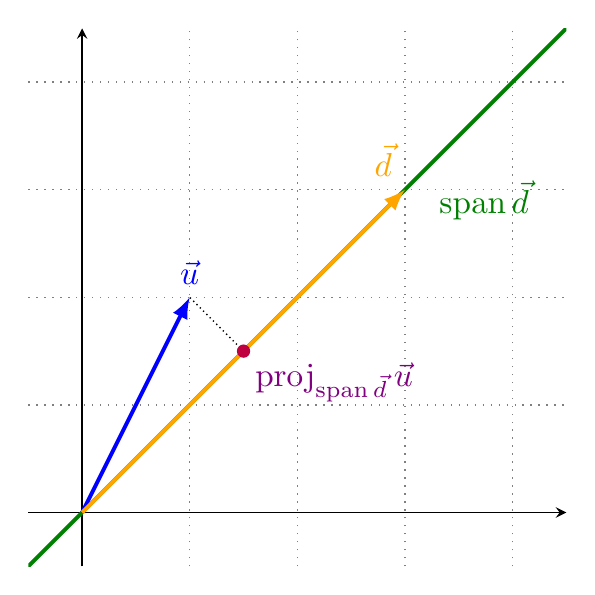
\begin{tikzpicture}[scale=1.2, >=latex]
			    \begin{axis}[scale=1,
					    axis equal image,
					    axis line style={black},
					    axis lines=middle,
					    tick style={draw=none},
					    yticklabels={,,},
					    xticklabels={,,},
					 xmin=-.5,
					 xmax=4.5,
					 ymin=-.5,
					 ymax=4.5,
					 major grid style={dotted, gray},
					 xtick={-10,-9,...,10},
					 ytick={-10,-9,...,10},
					 grid=both,
					 anchor=origin]

				    \draw[thin, densely dotted, black] (1.5,1.5) -- (1,2);
				    \draw[Green, very thick] (-1,-1) -- (5,5) node[pos=.7, below right] {$\Span\Set{\vec d}$};

				    \draw[blue, ->, very thick] (0,0) -- (1,2) node[above] {\color{blue}$\vec u$};
				    \draw[Orange, ->, very thick] (0,0) -- (3,3) node[above left] {\color{Orange}$\vec d$};
				    \fill[fill=purple] (1.5,1.5) circle[radius=2pt] node[below right] {\color{Purple}$\Proj_{\Span\Set{\vec d}}\vec u$};
			    \end{axis}
			\end{tikzpicture}
			\end{solution}
		\item How do $\Proj_{\Span\{\vec d\}}\vec u$ and $\Comp_{\vec d}\vec u$ relate?
			\begin{solution}[inline]
				They are equal.
			\end{solution}
		\item Compute $\Proj_{\Span\{\vec d\}}\vec u$ and $\Comp_{\vec d}\vec u$.
			\begin{solution}
				Using our formula from the previous problem
				\[
					\Proj_{\Span\{\vec d\}}\vec u
					=\Comp_{\vec d}\vec u
					=\frac{\vec u\cdot \vec d}{\norm{\vec d}^2} \vec d
					=\tfrac{9}{18}\vec d = \tfrac{1}{2}\mat{3\\3}.
				\]
			\end{solution}
		\item Compute $\Comp_{-\vec d}\vec u$. Is this the same as or different from
			$\Comp_{\vec d}\vec u$? Explain.
			\begin{solution}
				\[
					\Comp_{-\vec d}\vec u
					=\frac{\vec u\cdot (-\vec d)}{\norm{-\vec d}^2} (-\vec d)
					=\tfrac{-9}{18}(-\vec d) = \tfrac{1}{2}\mat{3\\3}
					=\Comp_{\vec d}\vec u.
				\]
				We expect them to be equal since $\vec d$ and $-\vec d$ are
				in the same direction as one another.
			\end{solution}
	\end{parts}


\begin{module}
	\Title{Subspaces \& Bases}

	In this module you will learn
	\begin{itemize}
		\item Formal and intuitive definitions of subspaces.
		\item The relationship between subspaces and spans.
		\item How to prove whether or not a set is a subspace.
		\item How to find a basis for and the dimension of a subspace.
	\end{itemize}

	Lines or planes through the origin can be written as spans
of their direction vectors. However, a line or plane that doesn't
pass through the origin cannot be written as a span---it must
be expressed as a \emph{translated} span.

\begin{center}
	\begin{tikzpicture}
		\begin{axis}[
		    anchor=origin,
		    disabledatascaling,
		    xmin=-2,xmax=4,
		    ymin=-1,ymax=3,
			xtick={-2,...,4},
		    x=1cm,y=1cm,
		    grid=both,
		    grid style={line width=.1pt, draw=gray!10},
		    %major grid style={line width=.2pt,draw=gray!50},
		    axis lines=middle,
		    minor tick num=0,
		    enlargelimits={abs=0.5},
		    axis line style={latex-latex},
		    ticklabel style={font=\tiny,fill=white},
		    xlabel style={at={(ticklabel* cs:1)},anchor=north west},
		    ylabel style={at={(ticklabel* cs:1)},anchor=south west}
		]

			\draw[myorange, very thick] (-4,-2) -- (6,3) node[pos=.35, below right, xshift=-7pt] {The span of $\vec d$};
			\draw[black, thick, dashed, ->] (0,0) -- (2,1) node[midway, below right] {$\vec d$};
			\draw[mygreen, thick] (-3,0) -- (5,4) node[near end, above left, xshift=8pt, yshift=-2pt] {Not a span, but a translated span};
		\end{axis}
	\end{tikzpicture}
\end{center}


There's something special about sets that can be expressed as 
(untranslated) spans. In particular, since a linear combination
of linear combinations is still a linear combination, a span
is \emph{closed} with respect to linear combinations. That is, 
by taking linear combinations of vectors in a span, you cannot
escape the span. In general, sets that have this property are called
\emph{subspaces}.

\SavedDefinitionRender{Subspace}

In the definition of a subspace, property (i) is called
	being \emph{closed with respect to vector addition} and
	property (ii) is called being \emph{closed with respect to
	scalar multiplication}.

Subspaces generalize the idea of \emph{flat spaces through the origin}. They include 
lines, planes, volumes and more.

\begin{example}
	Let $\mathcal V\subseteq \R^2$ be the complete solution to 
	$x+2y=0$.  Show that $\mathcal V$ is a subspace.
	
	Let $\vec u = \mat{u_1\\u_2}$ and 
	$\vec v = \mat{v_1\\v_2}$ be in $\mathcal V$, 
	and let $k$ be a scalar.
	
	By definition, we have 
	\[
	\begin{aligned}
		u_1+2u_2&=0 \\
		v_1+2v_2&=0
	\end{aligned}.
	\]
	
	We will show that $\mathcal V$ is nonempty and that
		(i) $\vec u + \vec v \in \mathcal V$; and
		(ii) $k\vec u \in \mathcal V$.
	
	First we will show (i).
	Observe that
	\[
		\vec u + \vec v = \mat{u_1+v_1\\u_2+v_2}
	\]
	and the coordinates of $\vec u+\vec v$ satisfy
	\[
		(u_1+v_1)+2(u_2+v_2)=
		(u_1+2u_2)+(v_1+2v_2)=
		0+0=0.
	\]
	Since the coordinates of $\vec u + \vec v$ satisfy the equation $x+2y=0$, 
	we have shown that $\vec u + \vec v \in \mathcal V$.
	
	Next we will show (ii).
	Observe that
	\[
		k\vec u = \mat{ku_1\\ku_2}
	\]
	and the coordinates of $k\vec u$ satisfy
	\[
		(ku_1)+2(ku_2) = 
		k(u_1+2u_2)=
		k0=0.
	\]
	And so, we have shown that $k\vec u \in \mathcal V$.
	
	Finally, since $\vec 0 = \mat{0\\0}$ satisfies $x+2y=0$, 
	we conclude that $\vec 0\in\mathcal V$
	and so $\mathcal V$ is non-empty.
	
	Thus, by the definition, we have shown that $\mathcal V$ is a subspace.	
\end{example}

\begin{example}
	Let $\mathcal W\subseteq \R^2$ be the line expressed in vector form
	as 
	\[
		\vec x=t\mat{1\\2}+\mat{1\\1}.
	\]
	Determine whether $\mathcal W$ is a subspace.

	$\mathcal W$ is \emph{not} a subspace. To see this, notice that $\vec v=\mat{1\\1}\in \mathcal W$,
	but $0\vec v=\vec 0\notin\mathcal W$. Therefore, $\mathcal W$ is not closed under scalar multiplication
	and so cannot be a subspace.
\end{example}


As mentioned earlier, subspaces and spans are deeply connected.
This connection is given by the following theorem.

\begin{theorem}[Subspace-Span]
	Every subspace is a span and every span is a subspace.  More precisely,
	$\mathcal V\subseteq \R^n$ is a subspace if and only if $\mathcal V=
	\Span\mathcal X$ for some set $\mathcal X$.
\end{theorem}
\begin{proof}
	We will start by showing every span is a subspace.  Fix $\mathcal X\subseteq\R^n$
	and let
	$\mathcal V=\Span\mathcal X$. First note that if $\mathcal X\neq \Set{}$, then $\mathcal V$
	is non-empty because $\mathcal X\subseteq\mathcal V$ and if $\mathcal X=\Set{}$, then $\mathcal V=\Set{\vec 0}$,
	and so is still non-empty.
	
	Fix $\vec v,\vec u\in\mathcal V$. By definition there are $\vec x_1,\vec x_2,\ldots,\vec y_1,\vec y_2,\ldots\in\mathcal X$ 
	and scalars $\alpha_1,\alpha_2,\ldots,\beta_1,\beta_2,\ldots$ so that
	\[
		\vec v=\sum \alpha_i\vec x_i\qquad \vec u=\sum\beta_i\vec y_i.
	\]

	To verify property (i), observe that
	\[
		\vec u+\vec v=\sum\alpha_i\vec x_i + \sum\beta_i\vec y_i
	\]
	is also a linear combination of vectors in $\mathcal X$ (because all $\vec x_i$ and $\vec y_i$
	are in $\mathcal X$), and so $\vec u+\vec v\in	\Span\mathcal X=\mathcal V$.
	
	To verify property (ii), observe that for any scalar $\alpha$, 
	\[
		\alpha\vec v=\alpha\sum \alpha_i\vec x_i = \sum (\alpha\alpha_i)\vec x_i\in
		\Span\mathcal X=\mathcal V.
	\]
	Since $\mathcal V$ is non-empty and satisfies both properties (i) and (ii), it is a subspace.

	Now we will prove that every subspace is a span. Let $\mathcal V$ be a subspace
	and consider $\mathcal V'=\Span\mathcal V$.  Since taking a span may only enlarge a set, we know
	$\mathcal V\subseteq \mathcal V'$. If we establish that $\mathcal V'\subseteq\mathcal V$,
	then $\mathcal V=\mathcal V'=\Span\mathcal V$, which would complete the proof.

	Fix $\vec x\in\mathcal V'$. By definition, there are $\vec v_1,\vec v_2,\ldots,\vec v_n\in\mathcal V$ and scalars
	$\alpha_1,\alpha_2,\ldots,\alpha_n$ so that
	\[
		\vec x=\sum \alpha_i\vec v_i.
	\]
	Observe that 
	$\alpha_i\vec v_i\in\mathcal V$ for all $i$, since $\mathcal V$ is closed under scalar
	multiplication. It follows that $\alpha_1\vec v_1+\alpha_2\vec v_2\in\mathcal V$,
	because $\mathcal V$ is closed under sums. Continuing, 
	$(\alpha_1\vec v_1+\alpha_2\vec v_2)+\alpha_3\vec v_3\in\mathcal V$ because
	$\mathcal V$ is closed under sums. Applying the principle of finite induction, we see
	\[
		\vec x=\sum \alpha_i\vec v_i
		=\Big(\big((\alpha_1\vec v_1+\alpha_2\vec v_2)
		+\alpha_3\vec v_3\big)+\cdots+\alpha_{n-1}\vec v_{n-1} \Big)
		+\alpha_n\vec v_n\in\mathcal V.
	\]
	Thus $\mathcal V'\subseteq\mathcal V$, which completes the proof.
\end{proof}

The previous theorem is saying that spans and subspaces are two ways of talking about the same
thing. Spans provide a \emph{constructive} definition of lines/planes/volumes/etc. through the origin. That is,
when you describe a line/plane/etc. through the origin as a span, you're saying ``this is a line/plane/etc. through the origin
because every point in it is a linear combination of \emph{these specific vectors}''. In contrast, subspaces provide a \emph{categorical}
definition of lines/planes/etc. through the origin. 
When you describe a line/plane/etc. through the origin as a subspace, 
you're saying ``this is a line/plane/etc. through the origin because these \emph{properties} are satisfied''\footnote{
Categorical definitions are useful when working with objects where it's hard to pin down exactly what the elements
inside are.}.


\begin{emphbox}[Takeaway]
	Spans and subspaces are two different ways of talking about the same objects: points/lines/planes/etc. through the origin.
\end{emphbox}

\Heading{Special Subspaces}
When thinking about $\R^n$, there are two special subspaces that are always available. The first is $\R^n$ itself.
$\R^n$ is obviously non-empty, and linear combinations of vectors in $\R^n$ remain in $\R^n$. The second is
the \emph{trivial subspace}, $\Set{\vec 0}$.

\SavedDefinitionRender{TrivialSubspace}

\begin{theorem}
	The trivial subspace is a subspace.
\end{theorem}
\begin{proof}
	First note that $\Set{\vec 0}$ is non-empty since $\vec 0\in\Set{\vec 0}$. Now, since
	$\vec 0$ is the only vector in $\Set{\vec 0}$, properties (i) and (ii) follow quickly:
	\[
		\vec 0+\vec 0=\vec 0\in \Set{\vec 0}
	\]
	and
	\[
		\alpha\vec 0=\vec 0\in\Set{\vec 0}.
	\]
\end{proof}

\Heading{Bases}

Let $\vec d=\mat{2\\1}$ and consider $\ell=\Span\Set{\vec d}$.

\begin{center}
	\begin{tikzpicture}
		\begin{axis}[
		    anchor=origin,
		    disabledatascaling,
		    xmin=-1,xmax=4,
		    ymin=-1,ymax=2,
			xtick={-2,...,4},
		    x=1cm,y=1cm,
		    grid=both,
		    grid style={line width=.1pt, draw=gray!10},
		    %major grid style={line width=.2pt,draw=gray!50},
		    axis lines=middle,
		    minor tick num=0,
		    enlargelimits={abs=0.5},
		    axis line style={latex-latex},
		    ticklabel style={font=\tiny,fill=white},
		    xlabel style={at={(ticklabel* cs:1)},anchor=north west},
		    ylabel style={at={(ticklabel* cs:1)},anchor=south west}
		]

			\draw[myorange, very thick] (-2,-1) -- (6,3) node[pos=.65, above left] {$\ell=\Span\Set{\vec d}$};
			\draw[black, thick, dashed, ->] (0,0) -- (2,1) node[midway, below right, yshift=2pt] {$\vec d$};
		\end{axis}
	\end{tikzpicture}
\end{center}

We know that $\ell$ is a subspace, and we defined $\ell$ as the span of $\Set{\vec d}$,
but we didn't have to define $\ell$ that way. We could have, for instance, defined $\ell=\Span\Set{\vec d,-2\vec d,\tfrac{1}{2}\vec d}$. However,
$\Span\Set{\vec d}$ is a simpler way to describe $\ell$ than $\Span\Set{\vec d,-2\vec d,\tfrac{1}{2}\vec d}$.
This property is general: the simplest descriptions of a line involve the span of only one vector.


Analogously, let $\mathcal P=\Span\Set{\vec d_1,\vec d_2}$ be the plane
through the origin with direction vectors $\vec d_1$ and $\vec d_2$. There
are many ways to write $\mathcal P$ as a span, but the simplest ones
involve exactly two vectors. The idea of a \emph{basis} comes
from trying to find the simplest description of a subspace.

\SavedDefinitionRender{Basis}

In short, a basis for a subspace is a linearly independent set that spans that
subspace.

\begin{example}
	\label{EXLINEBASIS}
	Let $\ell=\Span\Set*{\mat{1\\2},\mat{-2\\-4}, \mat{1/2\\1}}$. Find
	two different bases for $\ell$.
	
	We are looking for a set of linearly independent vectors that spans $\ell$.
	Notice that $\mat{1\\2} = -\tfrac{1}{2}\mat{-2\\-4} = 2\matc{1/2\\1}$.
	Therefore,
    \[
		\Span\Set*{\mat{1\\2}} =
		\Span\Set*{\mat{-2\\-4}} =
		\Span\Set*{\mat{1/2\\1}} =
		\Span\Set*{\mat{1\\2},\mat{-2\\-4}, \mat{1/2\\1}} =
		\ell.
	\]
	Because $\Set*{\mat{1\\2}}$ is linearly independent and spans $\ell$,
	we have that $\Set*{\mat{1\\2}}$ is a basis for $\ell$.
	Similarly, $\Set*{\matc{1/2\\1}}$ is another basis for $\ell$.
\end{example}

Unpacking the definition of basis a bit more, we can see that 
a basis for a subspace
 is a set of vectors
that is \emph{just the right size} to describe everything in the subspace.
It's not too big---because it is linearly independent, there are no
redundancies. It's not too small---because we require it to span the subspace\footnote{ 
If you're into British fairy tales, you might call a basis a \emph{Goldilocks set}.
}.

There are several facts everyone should know about bases:
\begin{enumerate}
	\item Bases are not unique. Every subspace (except the trivial subspace)
		has multiple bases.
	\item Given a basis for a subspace, every vector in the subspace can be written
		as a \emph{unique} linear combination of vectors in that basis.
	\item Any two bases for the same subspace have the same number of elements.
\end{enumerate}

You can prove the first fact by observing that if $\mathcal B=\Set{\vec b_1,\vec b_2,\ldots}$ is a basis
with at least one element\footnote{ The empty set is a basis for the trivial subspace.}, then
$\Set{2\vec b_1,2\vec b_2,\ldots}$ is a different basis. The second fact is a consequence of all bases 
being linearly independent. The third fact is less obvious and takes some legwork to prove, so we will accept it
as is.

\Heading{Dimension}

Let $\mathcal V$ be a subspace. Though there are many bases for $\mathcal V$, they all
have the same number of vectors in them. And, this number says something fundamental about $\mathcal V$:
it tells us the maximum number of linearly independent vectors that can simultaneously exist in $\mathcal V$.
We call this number the \emph{dimension} of $\mathcal V$.

\SavedDefinitionRender{Dimension}

This definition agrees with our intuition about lines and planes: the dimension of a line through $\vec 0$ is $1$, and
the dimension of a plane through $\vec 0$ is $2$. It even tells us the dimension of the single point $\Set{\vec 0}$
is $0$\footnote{ The dimension of a line, plane, or point
not through the origin is defined to be the dimension of the subspace obtained
when it is translated to the origin.}.

\begin{example}
	Find the dimension of $\R^2$.

	Since $\Set{\xhat, \yhat}$ is a basis for $\R^2$, we know $\R^2$ is
	two dimensional.
\end{example}

\begin{example}
	Let $\ell=\Span\Set*{\mat{1\\2},\mat{-2\\-4}, \mat{1/2\\1}}$.
	Find the dimension of the subspace $\ell$.

	This is the same subspace from the earlier example where we found
	$\Set*{\mat{1\\2}}$ and $\Set*{\matc{1/2\\1}}$
	were bases for $\ell$. Both these bases contain one element, and so
	$\ell$ is a one dimensional subspace.
\end{example}

\begin{example}
	Let $A=\Set{(x_1,x_2,x_3,x_4)\given x_1+2x_2-x_3=0\text{ and }x_1+6x_4=0}$. Find a basis for and the dimension
	of $A$.

	$A$ is the complete solution to the system
	\[
		\systeme{x_1+2x_2-x_3=0,x_1+6x_4=0},
	\]
	which can be expressed in vector form as
	\[
		\mat{x_1\\x_2\\x_3\\x_4} = t\matc{0\\1/2\\1\\0}+s\mat{-6\\3\\0\\1}.
	\]
	Therefore $A=\Span\Set*{\matc{0\\1/2\\1\\0}, \mat{-6\\3\\0\\1}}$. Since $\Set*{\matc{0\\1/2\\1\\0}, \mat{-6\\3\\0\\1}}$
	is a linearly independent spanning set with two elements, $A$ is two dimensional.
\end{example}

Like $\R^2$ and $\R^3$, whenever we discuss $\R^n$, we always have a standard basis that comes
along for the ride.

\SavedDefinitionRender{StandardBasisforRn}

Note: the notation $\vec e_i$ is context specific. If we say $\vec e_i\in\R^2$,
then $\vec e_i$ must have exactly two components. If we say $\vec e_i\in\R^{45}$,
then $\vec e_i$ must have $45$ components. 

\end{module}
	\bookonlynewpage
\section*{Subspaces and Bases}
	\vspace{-1em}
	\SavedDefinitionRender{Subspace}

	Subspaces give a mathematically precise definition of a ``flat space through the origin.''

	\question
	\begin{annotation}
		\begin{goals}
			\Goal{Visualizing subspaces.}

			The goal of this problem is to
			\begin{itemize}
				\item Read and apply the definition of subspace.
				\item Identify from a picture whether or not a set is a subspace.
				\item Write formal arguments showing whether or not certain sets are subspaces.
			\end{itemize}
		\end{goals}

		\begin{notes}
			Every part of this problem highlights a misconception or builds an abstraction.
			\begin{enumerate}
				\item[1.] Satisfies (i) but not (ii).
				\item[2.] Looks fairly flat, but violates (i) and (ii) in a specify way.
				\item[3.] First subspace.
				\item[4.] Looks flat, but violates (i) and (ii).
				\item[5.] Satisfies (ii) but not (i).
				\item[6.] Second subspace.
				\item[7.] Alternate notation which requires unpacking a definition.
				\item[8.] Abstractly defined subspace requires an abstract proof.
			\end{enumerate}
			\begin{itemize}
				\item Proving a set is a subset is one of the few \emph{proofs} we hold
					students accountable for, and they need practice. Remind them
					that to prove something is not a subspace they only need to
					prove that one condition is violated, and this can be done with
					an example. However, to prove something is a subspace, we need
					to make an argument about every single vector.
				\item Subspace proofs can follow a template. ``Let $\vec u,\vec v\in X$ and
					let $\alpha$ be a scalar. By definition \ldots, and so \ldots''. Let
					students try to write a proof on their own. Then, give them
					the template. Applying the template is harder than it seems, so
					emphasize for every subspace proof how it fits the template.
			\end{itemize}
		\end{notes}
	\end{annotation}
	For each set, draw it and explain whether or not it is a subspace of $\R^2$.
	\begin{parts}
		\item $A=\Set*{\vec x\in\R^2 \given \vec x=\mat{a\\0}\text{ for some }a\in\Z}$.
			\begin{solution}
			\begin{minipage}{.25\textwidth}
			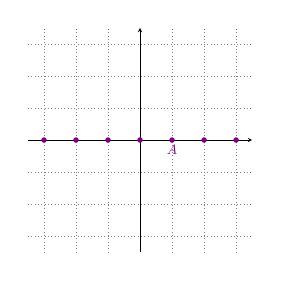
\begin{tikzpicture}[scale=.5, >=latex]
			    \begin{axis}[scale=1,
					    axis equal image,
					    axis line style={black},
					    axis lines=middle,
					    tick style={draw=none},
					    yticklabels={,,},
					    xticklabels={,,},
					 xmin=-3.5,
					 xmax=3.5,
					 ymin=-3.5,
					 ymax=3.5,
					 major grid style={dotted, gray},
					 xtick={-10,-9,...,10},
					 ytick={-10,-9,...,10},
					 grid=both,
					 anchor=origin]

				    \fill[fill=Purple] (1,0) circle[radius=2pt] node[below] {\color{Purple}$A$};
				    \fill[fill=Purple] (0,0) circle[radius=2pt];
				    \fill[fill=Purple] (-1,0) circle[radius=2pt];
				    \fill[fill=Purple] (-2,0) circle[radius=2pt];
				    \fill[fill=Purple] (-3,0) circle[radius=2pt];
				    \fill[fill=Purple] (2,0) circle[radius=2pt];
				    \fill[fill=Purple] (3,0) circle[radius=2pt];
			    \end{axis}
			\end{tikzpicture}
			\end{minipage}
			\begin{minipage}{.75\textwidth}

				$A$ is not a subspace, since for example $\mat{1\\0} \in A$ but
				$\frac{1}{2}\mat{1\\0}\notin A$.
			\end{minipage}
			\end{solution}
		\item $B=\Set*{\vec x\in\R^2 \given \vec x\neq \mat{0\\0}}$.
			\begin{solution}
				$B$ is not a subspace, since for example $\mat{1\\0}$ and $\mat{-1\\0}$
				are both in $B$, but their sum is $\mat{0\\0}$ which is not in $B$.
			\end{solution}
		\item $C=\Set*{\vec x\in\R^2 \given \vec x=\mat{0\\t}\text{ for some }t\in\R}$.
			\begin{solution}
			\begin{minipage}{.25\textwidth}
			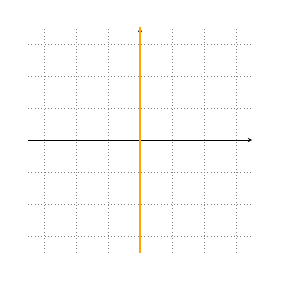
\begin{tikzpicture}[scale=.5, >=latex]
			    \begin{axis}[scale=1,
					    axis equal image,
					    axis line style={black},
					    axis lines=middle,
					    tick style={draw=none},
					    yticklabels={,,},
					    xticklabels={,,},
					 xmin=-3.5,
					 xmax=3.5,
					 ymin=-3.5,
					 ymax=3.5,
					 major grid style={dotted, gray},
					 xtick={-10,-9,...,10},
					 ytick={-10,-9,...,10},
					 grid=both,
					 anchor=origin]

				    \draw[Orange, very thick] (0,-4) -- (0,4);
			    \end{axis}
			\end{tikzpicture}
			\end{minipage}
			\begin{minipage}{.75\textwidth}

				$C$ is a subspace.

				\begin{enumerate}[label=(\roman*)]
					\item Let $\vec u,\vec v\in C$. Then $\vec u=\mat{0\\t}$ and
						$\vec v=\mat{0\\s}$ for some $s,t\in\R$.

						But then $\vec u+\vec v=\mat{0\\s+t}\in C$.
					\item Let $\vec u=\mat{0\\t}\in C$. For any scalar $\alpha$
						we have $\alpha\vec u=\mat{0\\\alpha t}\in C$.
				\end{enumerate}
			\end{minipage}
			\end{solution}
		\item $D=\Set*{\vec x\in\R^2 \given \vec x=\mat{0\\t}+\mat{1\\1}\text{ for some }t\in\R}$.
			\begin{solution}
			\begin{minipage}{.25\textwidth}
			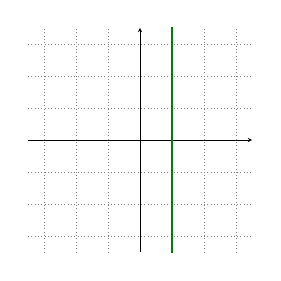
\begin{tikzpicture}[scale=.5, >=latex]
			    \begin{axis}[scale=1,
					    axis equal image,
					    axis line style={black},
					    axis lines=middle,
					    tick style={draw=none},
					    yticklabels={,,},
					    xticklabels={,,},
					 xmin=-3.5,
					 xmax=3.5,
					 ymin=-3.5,
					 ymax=3.5,
					 major grid style={dotted, gray},
					 xtick={-10,-9,...,10},
					 ytick={-10,-9,...,10},
					 grid=both,
					 anchor=origin]

				    \draw[Green, very thick] (1,-4) -- (1,4);
			    \end{axis}
			\end{tikzpicture}
			\end{minipage}
			\begin{minipage}{.75\textwidth}

				$D$ is not a subspace, since for example $\mat{1\\1}\in D$, but
				$0\mat{1\\1}=\mat{0\\0}\notin D$.
			\end{minipage}
			\end{solution}
		\item $E=\Set*{\vec x\in\R^2 \given \vec x=\mat{0\\t}\text{ or }\vec x=\mat{t\\0}\text{ for some }t\in\R}$.
			\begin{solution}
			\begin{minipage}{.25\textwidth}
			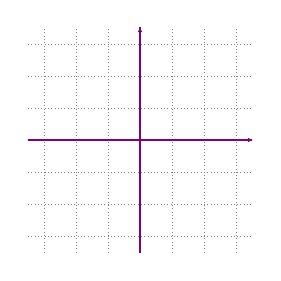
\begin{tikzpicture}[scale=.5, >=latex]
			    \begin{axis}[scale=1,
					    axis equal image,
					    axis line style={black},
					    axis lines=middle,
					    tick style={draw=none},
					    yticklabels={,,},
					    xticklabels={,,},
					 xmin=-3.5,
					 xmax=3.5,
					 ymin=-3.5,
					 ymax=3.5,
					 major grid style={dotted, gray},
					 xtick={-10,-9,...,10},
					 ytick={-10,-9,...,10},
					 grid=both,
					 anchor=origin]

				    \draw[Purple, very thick] (0,-4) -- (0,4);
				    \draw[Purple, very thick] (-4,0) -- (4,0);
			    \end{axis}
			\end{tikzpicture}
			\end{minipage}
			\begin{minipage}{.75\textwidth}

				$E$ is not a subspace, since for example  $\mat{1\\0}$ and $\mat{0\\1}$
				are both in $E$, but their sum is $\mat{1\\1}$ which is not in $E$.
			\end{minipage}
			\end{solution}
		\item $F=\Set*{\vec x\in\R^2 \given \vec x=t\mat{3\\1}\text{ for some }t\in\R}$.
			\begin{solution}
			\begin{minipage}{.25\textwidth}
			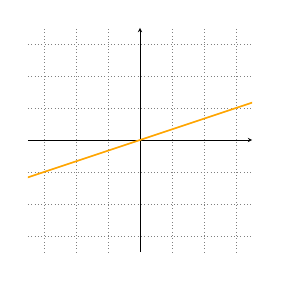
\begin{tikzpicture}[scale=.5, >=latex]
			    \begin{axis}[scale=1,
					    axis equal image,
					    axis line style={black},
					    axis lines=middle,
					    tick style={draw=none},
					    yticklabels={,,},
					    xticklabels={,,},
					 xmin=-3.5,
					 xmax=3.5,
					 ymin=-3.5,
					 ymax=3.5,
					 major grid style={dotted, gray},
					 xtick={-10,-9,...,10},
					 ytick={-10,-9,...,10},
					 grid=both,
					 anchor=origin]

				    \draw[Orange, very thick] (6,2) -- (-6,-2);
			    \end{axis}
			\end{tikzpicture}
			\end{minipage}
			\begin{minipage}{.75\textwidth}
				$F$ is a subspace.

				\begin{enumerate}[label=(\roman*)]
					\item Let $\vec u,\vec v\in F$. Then $\vec u=t\mat{3\\1}$ and
						$\vec v=s\mat{3\\1}$ for some $s,t\in\R$.

						But then $\vec u+\vec v=(s+t)\mat{3\\1}\in F$.
					\item Let $\vec u=t\mat{3\\1}\in F$. For any scalar $\alpha$
						we have $\alpha\vec u=(\alpha t)\mat{3\\1}\in F$.
				\end{enumerate}
			\end{minipage}
			\end{solution}
		\item $G=\Span\left\{\mat{1\\1}\right\}$.
			\begin{solution}
			\begin{minipage}{.25\textwidth}
			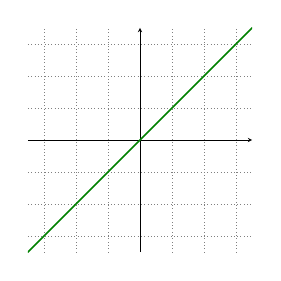
\begin{tikzpicture}[scale=.5, >=latex]
			    \begin{axis}[scale=1,
					    axis equal image,
					    axis line style={black},
					    axis lines=middle,
					    tick style={draw=none},
					    yticklabels={,,},
					    xticklabels={,,},
					 xmin=-3.5,
					 xmax=3.5,
					 ymin=-3.5,
					 ymax=3.5,
					 major grid style={dotted, gray},
					 xtick={-10,-9,...,10},
					 ytick={-10,-9,...,10},
					 grid=both,
					 anchor=origin]

				    \draw[Green, very thick] (-4,-4) -- (4,4);
			    \end{axis}
			\end{tikzpicture}
			\end{minipage}
			\begin{minipage}{.75\textwidth}

				$G$ is a subspace.

				By definition of a span,
				$G=\Set*{\vec x\in\R^2 \given \vec x=t\mat{1\\1}\text{ for some }t\in\R}$.

				The proof that $G$ is a subspace now proceeds similarly to the
				proof for $F$ above.

				\begin{enumerate}[label=(\roman*)]
					\item Let $\vec u,\vec v\in G$. Then $\vec u=t\mat{1\\1}$ and
						$\vec v=s\mat{1\\1}$ for some $s,t\in\R$.

						But then $\vec u+\vec v=(s+t)\mat{1\\1}\in G$.
					\item Let $\vec u=t\mat{1\\1}\in G$. For any scalar $\alpha$
						we have $\alpha\vec u=(\alpha t)\mat{1\\1}\in G$.
				\end{enumerate}
			\end{minipage}

		\end{solution}
		\item $H=\Span\Set{\vec u,\vec v}$ for some unknown vectors $\vec u,\vec v\in\R^2$.
			\begin{solution}
				$H$ is a subspace.

				\begin{enumerate}[label=(\roman*)]
					\item Let $\vec x,\vec y\in H$.
						Then $\vec x=\alpha_1\vec u+\alpha_2\vec v$ and
						$\vec y=\beta_1\vec u+\beta_2\vec v$ for some scalars
						$\alpha_1,\alpha_2,\beta_1,\beta_2$. But then
						\[
							\vec x+\vec y
							=\alpha_1\vec u+\alpha_2\vec v+\beta_1\vec u+\beta_2\vec v
							=(\alpha_1+\beta_1)\vec u+(\alpha_2+\beta_2)\vec v\in H.
						\]

					\item Let $\vec x=\alpha_1\vec u+\alpha_2\vec v\in H$.
						For any	scalar $\beta$ we have
						$\beta\vec u=(\beta\alpha_1)\vec u+(\beta\alpha_2)\vec v\in H$.
				\end{enumerate}
			\end{solution}
	\end{parts}

\begin{lesson}
	\Title{Basis, Dimension}

	\Heading{Textbook}
	Sections 1.2, 4.3

	\Heading{Objectives}
	\begin{itemize}
		\item Define Basis.
		\item Define Dimension.
		\item Find a basis for a subspace.
		\item Find the dimension of a subspace.
	\end{itemize}

	\Heading{Motivation}
	Bases are sets of just enough vectors to describe every vector in a subspace.
	An additional consequence of a basis is that every vector can be \emph{uniquely}
	represented as a linear combination of basis vectors. Using this fact we
	will be able to consider objects in multiple different coordinate systems. However,
	now is the time to get familiar with what a basis is and how to find one.

	Dimension ties the abstract notion of subspace to our intuition about
	Euclidean space. We already know a plane in $\R^3$ is two dimensional,
	but now we know where that number \emph{two} comes from.

\end{lesson}
	\bookonlynewpage
	\SavedDefinitionRender{Basis}
	\SavedDefinitionRender{Dimension}


	\question
	\begin{annotation}
		\begin{goals}
			\Goal{Apply the definitions of basis and dimension to a simple example.}

			The goal of this problem is to learn
			\begin{itemize}
				\item To apply the definition of basis and dimension.
				\item Intuition that a plane is two dimensional.
				\item A basis is not unique, but always has the same size (this is not proved).
				\item Spans are never bases---you must not confuse a subspace with its basis!
			\end{itemize}
		\end{goals}

		\begin{notes}
			\begin{itemize}
				\item Students will claim $V$ is $\R^2$ and fail to distinguish
					$\R^2$ and the $xy$-plane in $\R^3$.
				\item Parts 2, 3, 4, 6 will be easy; don't belabor them.
				\item Students will fail to distinguish $\Span\{\vec u,\vec v\}$
					from $\{\vec u,\vec v\}$. Make sure this distinction comes out.
			\end{itemize}
		\end{notes}
	\end{annotation}
	Let $\vec u=\mat{1\\0\\0}$, $\vec v=\mat{0\\1\\0}$, $\vec w=\mat{1\\1\\0}$,
	and $V=\Span\Set{\vec u,\vec v,\vec w}$.
	\begin{parts}
		\item Describe $V$.
			\begin{solution}[inline]
				$V$ is the $xy$-plane in $\R^3$.
			\end{solution}
		\item Is $\Set{\vec u,\vec v,\vec w}$ a basis for $V$?  Why or why not?
			\begin{solution}
				No. The set $\Set{\vec u,\vec v,\vec w}$ is linearly dependent since $\vec w=\vec u+\vec v$.
			\end{solution}
		\item Give a basis for $V$.
			\begin{solution}[inline]
				$\Set{\vec u,\vec v}$.
			\end{solution}
		\item Give another basis for $V$.
			\begin{solution}[inline]
				$\Set{\vec u,\vec w}$ or $\Set{\vec v,\vec w}$.
			\end{solution}
		\item Is $\Span\Set{\vec u,\vec v}$ a basis for $V$?  Why or why not?
			\begin{solution}
				No. $\Span\Set{\vec u,\vec v}$ is an infinite set of vectors
				which includes $\vec 0$, so it cannot be linearly independent and
				therefore isn't a basis.
			\end{solution}
		\item What is the dimension of $V$?
			\begin{solution}
				A basis for $V$ has two vectors so it is two-dimensional. We also
				know this because $V$ is the $xy$-plane in $\R^3$ and all planes
				are two-dimensional.
			\end{solution}
	\end{parts}

	\bookonlynewpage
	\question
	\begin{annotation}
		\begin{goals}
			\Goal{The relationship between subspaces, bases, unions, and intersections.}

			The goal of this problem is to learn
			\begin{itemize}
				\item Recognize intersections of subspaces as subspaces.
				\item Recognize the union of subspaces need not be a subspace.
				\item Visualize planes in $\R^3$ to solve problems without computations.
			\end{itemize}
		\end{goals}

		\begin{notes}
			\begin{itemize}
				\item Remind students that if they're stuck, they can always create a system
					of equations to help answer their question.
				\item For part 3, students could row-reduce if they're stuck, but the nicer
					way is to notice $\vec b$ is common to both spans and so, since the
					planes are not parallel, their intersection must be the line $\Span\Set{\vec b}$.
				\item Part 4 is hard to prove, but you can make a hand-wavy argument without
					too much trouble. Don't worry about getting a rock-solid proof for this part.
			\end{itemize}
		\end{notes}
	\end{annotation}
	Let $\vec a=\mat{1\\2\\3}$, $\vec b=\mat{4\\5\\6}$, $\vec c=\mat{7\\8\\8}$ (notice these vectors
	are linearly independent) and
	let $P=\Span\Set{\vec a,\vec b}$ and $Q=\Span\Set{\vec b,\vec c}$.
	\begin{parts}
		\item Give a basis for and the dimension of $P$.
			\begin{solution}
				$\Set{\vec a,\vec b}$ is a basis for $P$, and so its dimension is 2.
			\end{solution}
		\item Give a basis for and the dimension of $Q$.
			\begin{solution}
				$\Set{\vec b,\vec c}$ is a basis for $Q$, and so its dimension is 2.
			\end{solution}
		\item Is $P\cap Q$ a subspace? If so, give a basis for it and its dimension.
			\begin{solution}
				Yes. $\Set{\vec b}$ is a basis for $P\cap Q$, and so its dimension is 1.

				$P$ and $Q$ are both planes and are not parallel (since
				$\vec a,\vec b,\vec c$ are linearly independent). The intersection
				of any two non-parallel	planes in $\R^3$ is a line.
				We know that $\vec 0$ and $\vec b$ are on this line, and therefore
				the line is $\Span\Set{\vec b}$
			\end{solution}
		\item Is $P\cup Q$ a subspace? If so, give a basis for it and its dimension.
			\begin{solution}
				No. For example $\vec a$ and $\vec c$ are both in $P\cup Q$, but
				$\vec a+\vec c \notin P\cup Q$.

				Proof: A vector is in $P\cup Q$ if it is in $P$ or $Q$, so we must show
				that $\vec a+\vec c\notin P$ and $\vec a+\vec c\notin Q$

				$\vec a+\vec c \notin P$ since if it were, we would also have
				$(\vec a+\vec c)-\vec a=\vec c\in P$. We know this is impossible
				since the vectors $\vec a,\vec b,\vec c$ are linearly independent,
				and so $\vec c$ does not equal a linear combination of $\vec a$
				and $\vec b$.

				An analogous argument shows that $\vec a+\vec c \notin Q$.
			\end{solution}
	\end{parts}

\begin{module}
	\Title{Matrix Representations of Systems of Linear Equations}

	In this module you will learn
	\begin{itemize}
		\item How to represent a system of linear equations as a matrix equation.
		\item Multiple ways to interpret solutions of systems of linear equations.
		\item How linear independence/dependence relates to solutions to matrix equations.
		\item How to use matrix equations to find normal vectors to lines or planes.
	\end{itemize}
	
	\input{modules/module7.tex}
\end{module}
\begin{lesson}
	\Title{Matrices}

	\Heading{Textbook}
	Section 3.1

	\Heading{Objectives}
	\begin{itemize}
		\item Write a system of linear equations as a matrix equation.
		\item Write a matrix equation as a system of linear equations.
		\item Pose familiar problems (e.g., ``find a normal vector'', or
			``do these planes intersect\mbox{?}'') as matrix-equation
			questions.
	\end{itemize}

	\Heading{Motivation}
	Matrices will soon become a powerful tool to study linear transformations.
	However, we will start out viewing them as a notation to represent
	systems of linear equations. The fact that matrix-vector multiplication
	has two interpretations, as a linear combination of columns or as a dot product
	with rows, already connects geometry and angles with questions about linear combinations.

\end{lesson}
	\bookonlynewpage
\section*{Matrices}

	\question
	\begin{annotation}
		\begin{goals}
			\Goal{Relate matrix equations and systems of linear equations.}

			The goal of this problem is to
			\begin{itemize}
				\item Use matrix-vector multiplication to represent a system of equations
					with compact notation.
				\item View a matrix equation as a statement about (i) linear combinations of column vectors
					and (ii) a system of equations coming from the rows.
			\end{itemize}
		\end{goals}

		\begin{notes}
			\begin{itemize}
				\item Students know two different interpretations of matrix multiplication from
					the homework.
			\end{itemize}
		\end{notes}
	\end{annotation}
	Let $A=\mat{1&2\\3&3}$, $\vec x=\mat{x\\y}$, and $\vec b=\mat{-2\\-1}$.
	\begin{parts}
		\item Compute the product $A\vec x$.
			\begin{solution}
				$A \vec x = \mat{x+2y\\3x+3y}$.
			\end{solution}
		\item Write down a system of equations that corresponds to the matrix equation
			$A\vec x=\vec b$.
			\begin{solution}
				\begin{align*}
					x + 2y &= -2 \\
					3x + 3y &= -1
				\end{align*}
			\end{solution}
		\item Let $\mat{x_0\\y_0}$ be a solution to $A\vec x=\vec b$. Explain what
			$x_0$ and $y_0$ mean in terms of \emph{linear combinations} (hint: think
			about the columns of $A$).
			\begin{solution}
				$x_0$ and $y_0$, when used as scalars in a linear combination of
				the columns of $A$, make the vector $\vec b$. In other words:
				\[
					x_0 \mat{1\\3} + y_0 \mat{2\\3} = \mat{-2\\-1}.
				\]
			\end{solution}
		\item Let $\mat{x_0\\y_0}$ be a solution to $A\vec x=\vec b$. Explain what
			$x_0$ and $y_0$ mean in terms of \emph{intersecting lines} (hint: think
			about systems of equations).
			\begin{solution}
				The lines represented by the equations $x+2y=-2$ and $3x+3y=-1$
				from the system of equations above intersect at the point $\mat{x_0\\y_0}$.
			\end{solution}
	\end{parts}

	\bookonlynewpage
	\question
	\begin{annotation}
		\begin{goals}
			\Goal{Rephrase previous questions using matrix equations.}

			The goal of this problem is to
			\begin{itemize}
				\item Rephrase the question of linear independence as the special
					matrix equation $A\vec x=\vec 0$.
			\end{itemize}
		\end{goals}

		\begin{notes}
			\begin{itemize}
				\item We haven't formally introduced the term \emph{homogeneous system}
					yet. Now is a good time. The equation $A\vec x=\vec 0$ will be used
					again when talking about null spaces.
			\end{itemize}
		\end{notes}
	\end{annotation}
	Let $\vec u=\mat{1\\2\\3}$, $\vec v=\mat{4\\5\\6}$, $\vec w=\mat{7\\8\\9}$.
	\begin{parts}
		\item How could you determine if $\Set{\vec u,\vec v,\vec w}$ was a linearly
			independent set?
			\begin{solution}
				The set is linearly independent if and only if no non-trivial linear
				combination of the vectors $\vec u,\vec v,\vec w$ equals $\vec 0$.
				That is, if $x, y, z$ are scalars such that
				$x\vec u+y\vec v+z\vec w=\vec 0$, then $x=y=z=0$.

				In other words, the only solution of the following
				system of equations is $x=y=z=0$.
				\begin{align*}
					x + 4y + 7z &= 0 \\
					2x + 5y + 8z &= 0 \\
					3x + 6y + 9z &= 0 \\
				\end{align*}
			\end{solution}
		\item Can your method be rephrased in terms of a matrix equation? Explain.
			\begin{solution}
				The system of linear equations above can be represented by the
				matrix equation $A\vec x = \vec 0$, where $A = \mat{1&4&7\\2&5&8\\3&6&9}$
				and $\vec x=\mat{x\\y\\z}$.

				So another way to say the above is that the set is linearly independent
				if and only if the only solution to the equation $A \vec x = \vec 0$
				is $\vec x = \vec 0$.
			\end{solution}
	\end{parts}


	\bookonlynewpage
	\question
	\begin{annotation}
		\begin{goals}
			\Goal{Interpret matrix equations.}

			The goal of this problem is to
			\begin{itemize}
				\item Use knowledge about systems of linear equations to answer questions
					about matrix equations.
			\end{itemize}
		\end{goals}

		\begin{notes}
			\begin{itemize}
				\item This is mainly an exercise in applying existing knowledge about
					interpreting RREF to matrix equations.
			\end{itemize}
		\end{notes}
	\end{annotation}
	Consider the system represented by
	\[
		\mat{1&-3&0\\0&0&1\\0&0&0}\mat{x\\y\\z}=\vec b.
	\]
	\begin{parts}
		\item If $\vec b=\mat{1\\2\\3}$, is the set of solutions to this system
			a point, line, plane, or other?
			\begin{solution}
				This system has no solutions, since, if we expand the matrix
				equation into a system of equations, the third equation would be
				$0=3$, which is impossible.
			\end{solution}
		\item If $\vec b=\mat{1\\1\\0}$, is the set of solutions to this system
			a point, line, plane, or other?
			\begin{solution}
				A line. The system would be
				\begin{align*}
					x - 3y &= 1 \\
					z &= 1 \\
					0 &= 0
				\end{align*}
				A vector $\vec x=\mat{x\\y\\z}$ that satisfies this system must have
				$z=1$, and by the first equation in the system any value of $x$
				determines the value of $y$, and vice versa. In other words the
				system has one free variable, and so its set of solutions is a line.
			\end{solution}
	\end{parts}

	\bookonlynewpage
	\question
	\begin{annotation}
		\begin{goals}
			\Goal{Apply matrix equations to planes.}

			The goal of this problem is to
			\begin{itemize}
				\item Rephrase properties of a plane in terms of matrix equations.
				\item Be able to describe one application of the transpose.
			\end{itemize}
		\end{goals}

		\begin{notes}
			\begin{itemize}
				\item We are using the range of a matrix operator to describe a plane and the
					null space of a matrix to define normal vectors.
				\item Part 2 admits some trivial answers, but the interesting one is when 
					the range is $\mathcal P$.
				\item For part 3, students might miss the $\vec n\neq \vec 0$ condition.
				\item The matrices $K$ and $M$ do not have to be transposes of each other,
					but arrange it so they are.
			\end{itemize}
		\end{notes}
	\end{annotation}
	Let $\vec d_1=\mat{1\\1\\2}$ and $\vec d_2=\mat{-1\\1\\0}$.
	Let $\mathcal P$ be the plane given in vector form by $\vec x=t\vec d_1+s\vec d_2$.
	Further, suppose $M$ is a matrix so that $M\vec r\in\mathcal P$ for any $\vec r\in\R^2$.
	\begin{parts}
		\item How many rows does $M$ have?
			\begin{solution}
				Three. It must have three rows in order for $M\vec r$ to be an
				element of $\R^3$.
			\end{solution}
		\item Find such an $M$.
			\begin{solution}
				$M=\mat{1&-1\\1&1\\2&0}$ is one possible answer, since if
				$\vec r = \mat{a\\b}$, then $M \vec r = a \vec d_1 + b \vec d_2$.

				Another less interesting answer is the $3\times2$ zero matrix.
			\end{solution}
		\item Find necessary and sufficient conditions (phrased as equations) for
			$\vec n$ to be a normal vector for $\mathcal P$.
			\begin{solution}
				$\vec n$ is normal to $\mathcal P$ if and only if $\vec n\neq \vec 0$,
				$\vec n\cdot\vec d_1=0$, \emph{and} $\vec n\cdot\vec d_2=0$
			\end{solution}
		\item Find a matrix $K$ so that non-zero solutions to $K\vec x=\vec 0$ are normal
			vectors for $\mathcal P$. How do $K$ and $M$ relate?
			\begin{solution}
				$K = \mat{1&1&2\\-1&1&0}$. $K$ and $M$ are transposes of
				one another.

				The conditions $\vec n\cdot\vec d_1=0$ and $\vec n\cdot\vec d_2=0$
				from the previous part translate to the following system of equations:
				\begin{align*}
					x + y + 2z &= 0 \\
					-x + y &= 0.
				\end{align*}
				This system of equations can be represented by the matrix equation
				\[
					\mat{1&1&2\\-1&1&0}\mat{x\\y\\z} = \mat{0\\0}.
				\]
			\end{solution}
	\end{parts}


\begin{module}
	\Title{Coordinates \& Change of Basis I}

	In this module you will learn
	\begin{itemize}
		\item Notation for representing a vector in multiple bases.
		\item The distinction between a vector and its representation.
		\item How to compute multiple representation of a vector.
		\item The definition of an \emph{oriented} basis.
	\end{itemize}

	\input{modules/module8.tex}
\end{module}
\begin{lesson}
	\Title{Change of Basis I}

	\Heading{Textbook}
	Section 4.4

	\Heading{Objectives}
	\begin{itemize}
		\item Write a vector in multiple bases.
		\item Explain what the notation $[\vec v]_{\mathcal B}$ means.
		\item Explain what the notation $\mat{a\\b\\c}_{\mathcal B}$ means.
	\end{itemize}

	\Heading{Motivation}
	One of the most useful ideas in linear algebra is that you can
	represent a vector, a geometric object, with a list of numbers. This
	is done by picking a basis. So far we've implicitly used the standard basis,
	but now we're going to use other bases.

	\begin{annotation}
		\begin{notes}
			So far, we have written $\mat{1\\1}$ to mean
			$\mat{1\\1}_{\mathcal E}$ where $\mathcal E$ is the
			standard basis. We will continue to do this as convenient,
			but if multiple bases are ever involved, we will be careful
			to specify the basis.
		\end{notes}
	\end{annotation}
	Now lists of numbers can mean many different things and can be identified
	with vectors in many ways, so we need some notation to keep things straight.
	It's important now to distinguish when something is a list of numbers (a matrix)
	and when it is a vector. This distinction will arise again when
	we talk about linear transformations and their matrix representations.

\end{lesson}
	\bookonlynewpage
\section*{Change of Basis \& Coordinates}

	\question
	\begin{annotation}
		\begin{goals}
			\Goal{Motivate change of basis.}

			The goal of this problem is to
			\begin{itemize}
				\item Describe points in multiple bases when given a visual description of the basis
					or when given the basis vectors numerically.
				\item Recognize ambiguity when faced with the question, ``Which basis is better?''
			\end{itemize}
		\end{goals}

		\begin{notes}
			\begin{itemize}
				\item The Oronto streets are set up like 3,4,5 right triangle and all the numbers are easy.
					This question can be answered from the picture or algebraically.
				\item Part 4 is important. A convincing argument is that one basis is not intrinsically
					``better'' than the other is that if the compass rose were
					not shown, you couldn't tell from the picture which way was north (since the streets are orthogonal
					to each other just like north and east are)!

					Emphasize that the ``best'' representation of a point will depend on what
					question you're trying to answer.
			\end{itemize}
		\end{notes}
	\end{annotation}
	The fictional town of Oronto is not aligned with the usual
	compass directions. The streets are laid out as follows:

\begin{center}
	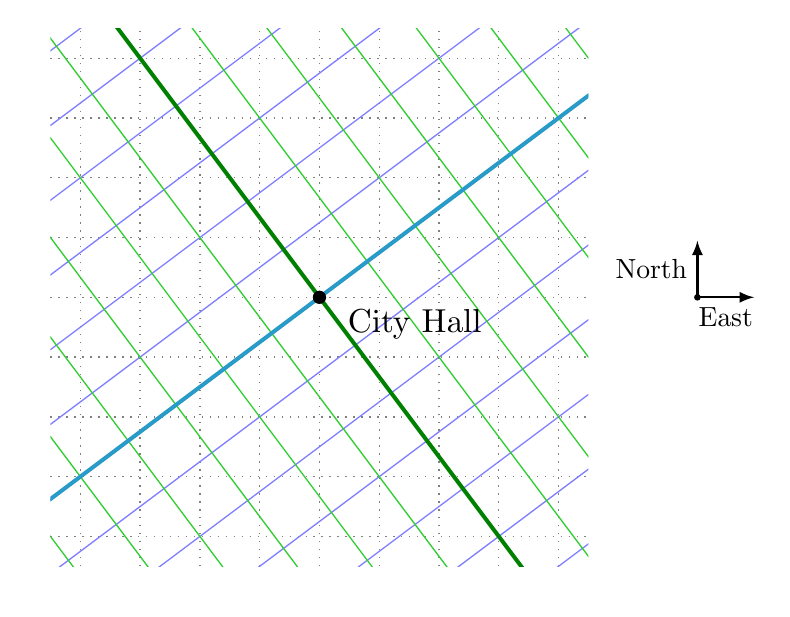
\begin{tikzpicture}[scale=1.2, >=latex]
    \begin{axis}[scale=1,
		    axis equal image,
		    axis line style={draw=none},
		    tick style={draw=none},
		    yticklabels={,,},
		    xticklabels={,,},
		 xmin=-4.5,
		 xmax=4.5,
		 ymin=-4.5,
		 ymax=4.5,
		 major grid style={dotted, gray},
                 xtick={-10,-9,...,10},
                 ytick={-10,-9,...,10},
                 grid=both,
		 anchor=origin]

	    \foreach \ival in {-6,...,6} {
	    	\edef\temp{\noexpand\draw[blue!50!white] (-8-0.6*\ival,-6+0.8*\ival) -- (8-0.6*\ival,6+.8*\ival);}
		\temp
	    }
	    \foreach \ival in {-6,...,6} {
	    	\edef\temp{\noexpand\draw[LimeGreen] (-6+0.8*\ival,8+0.6*\ival) -- (6+0.8*\ival,-8+0.6*\ival);}
		\temp
	    }
	    \draw[Green, very thick] (-6,8) -- (6,-8);
	    \draw[cyan!80!black, very thick] (-8,-6) -- (8,6);


	  \fill[fill=black] (0,0) circle[radius=2pt] node[below right, xshift=5pt] {City Hall};
    \end{axis}
		\draw[->, thick] (4,0) -- (4,.6) node[midway, left] {North};
		\draw[->, thick] (4,0) -- (4.6,0) node[midway, below] {East};
	  \fill[fill=black] (4,0) circle[radius=1pt];
\end{tikzpicture}
\end{center}


	Instead, every street is parallel to the vector
	$\vec d_1=\frac{1}{5}\mat{4\text{ east}\\3\text{ north}}$ or
	$\vec d_2=\tfrac{1}{5}\mat{-3\text{ east}\\4\text{ north}}$. The center of
	town is City Hall at $\vec 0=\mat{0\text{ east}\\0\text{ north}}$.

	Locations in Oronto are typically specified in \emph{street coordinates}. That
	is, as a pair $(a,b)$ where $a$ is how far you walk along streets in the $\vec d_1$ direction
	and $b$ is how far you walk in the $\vec d_2$ direction, provided you start at city hall.

	\begin{parts}
		\item The points $A=(2,1)$ and $B=(3,-1)$ are given in street coordinates.
			Find their east-north coordinates.
			\begin{solution}
				$A=(1,2)$ and $B=(3,1)$ in east-north coordinates.

				We obtain $A$ for example by finding the vector $2\vec d_1+\vec d_2$.
			\end{solution}
		\item The points $X=(4,3)$ and $Y=(1,7)$ are given in east-north coordinates.
			Find their street coordinates.
			\begin{solution}[inline]
				$X=(5,0)$ and $Y=(5,5)$ in street coordinates.
			\end{solution}
		\item Define $\vec e_1=\mat{1\text{ east}\\0\text{ north}}$ and
			$\vec e_2=\mat{0\text{ east}\\1\text{ north}}$.
			Does $\Span\Set{\vec e_1,\vec e_2} = \Span\Set{\vec d_1,\vec d_2}$?
			\begin{solution}
				Yes. Both of these sets spans all of $\R^2$.
			\end{solution}
		\item Notice that $Y=5\vec d_1+5\vec d_2 = \vec e_1+7\vec e_2$. Is the point $Y$
			better represented by the pair $(5,5)$ or by the pair $(1,7)$? Explain.
			\begin{solution}
				It is equally well represented by either pair. For example, the
				street coordinates might be more useful for a resident of Oronto,
				while the east-north coordinates might be more useful for someone
				looking at Oronto on a world map.
			\end{solution}
	\end{parts}

\displayonlynewpage
	\bookonlynewpage
	\SavedDefinitionRender{RepresentationinaBasis}

	\question
	\begin{annotation}
		\begin{goals}
			\Goal{Change of basis notation.}

			The goal of this problem is to
		\displayonlynewpage
			\begin{itemize}
				\item Practice using change-of-basis notation.
				\item Compute representations of vectors in different bases.
				\item Find a matrix that computes a change of basis.
			\end{itemize}
		\end{goals}

		\begin{notes}
			\begin{itemize}
				\item Up to this point, we have been sloppy, writing $\mat{1\\2}$ when
					we mean $\mat{1\\2}_{\mathcal C}$. For this problem, be precise.
					Unscripted matrices are boxes of numbers with no meaning other
					than what we give them. Subscripted matrices are actual vectors.

					We will be sloppy again in the future---if we interpret $\mat{1\\2}$
					as a vector, we will always assume it is $\mat{1\\2}_{\mathcal E}$ unless
					specified otherwise. But, at the start of change-of-basis, we will be careful.
				\item For part 5, we do not know about inverse matrices yet. This question should
					be answered from first principles.
				\item It will be hard for students to get their head around this notation. $\mat{1\\2}$ and $[\vec v]_{\mathcal X}$
					are boxes of numbers while $\vec v$ and $\mat{1\\2}_{\mathcal X}$ are vectors.
			\end{itemize}
		\end{notes}
	\end{annotation}
	Let $\mathcal E=\Set{\xhat,\yhat}$ be the standard basis for $\R^2$ and
	let $\mathcal C=\Set{\vec c_1,\vec c_2}$ where $\vec c_1=\mat{2\\1}_{\mathcal E}$
	and $\vec c_2=\mat{5\\3}_{\mathcal E}$ be another basis for $\R^2$.
	\begin{parts}
		\item Express $\vec c_1$ and $\vec c_2$ as a linear combination of $\xhat$ and $\yhat$.
			\begin{solution}[inline]
				$\vec c_1=2\xhat+\yhat$ and $\vec c_2=5\xhat+3\yhat$.
			\end{solution}
		\item Express $\xhat$ and $\yhat$ as a linear combination of $\vec c_1$ and $\vec c_2$.
			\begin{solution}[inline]
				$\xhat=3\vec c_1-\vec c_2$ and $\yhat=-5\vec c_1+2\vec c_2$.
			\end{solution}
		\item Let $\vec v=2\xhat+2\yhat$. Find $[\vec v]_{\mathcal E}$ and $[\vec v]_{\mathcal C}$.
			\begin{solution}
				$[\vec v]_{\mathcal E} = \mat{2\\2}$ and
				$[\vec v]_{\mathcal C} = \mat{-4\\2}$.

				The second one is since
				\[
					\vec v=2\xhat+2\yhat
					=2(3\vec c_1-\vec c_2)+2(-5\vec c_1+2\vec c_2)
					=-4\vec c_1+2\vec c_2.
				\]
			\end{solution}
		\item Can you find a matrix $X$ so that $X[\vec w]_{\mathcal C} = [\vec w]_{\mathcal E}$
			for any	$\vec w$?
			\begin{solution}
				$X = \mat{2&5\\1&3}$ is such a matrix.

				We know $X$ must be a $2\times2$ matrix, so suppose $X=\mat{a&b\\c&b}$
				for some $a,b,c,d\in\R$.

				From the first part above, we know
				\[
					\mat{1\\0}_{\mathcal C} = \mat{2\\1}_{\mathcal E}
					\quad \text{and} \quad
					\mat{0\\1}_{\mathcal C} = \mat{5\\3}_{\mathcal E},
				\]
				and so we need $X$ to satisfy
				\[
					X\mat{1\\0}=\mat{2\\1}
					\quad \text{and} \quad
					X\mat{0\\1}=\mat{5\\3}.
				\]
				But $X\mat{1\\0}=\mat{a\\c}$ and $X\mat{0\\1}=\mat{b\\d}$, so we
				can now immediately solve for $a,b,c,d$ to find that $X$ must be
				the matrix $\mat{2&5\\1&3}$.
			\end{solution}
		\item Can you find a matrix $Y$ so that $Y[\vec w]_{\mathcal E} = [\vec w]_{\mathcal C}$
			for any	$\vec w$?
			\begin{solution}
				$Y = \mat{3&-5\\-1&2}$ is such a matrix.

				Using similar reasoning to the previous part, we know $Y$ must be
				a $2\times2$ matrix, so suppose $Y=\mat{a&b\\c&b}$ for some
				$a,b,c,d\in\R$.

				From the second part above, we know
				\[
					\mat{1\\0}_{\mathcal E} = \mat{3\\-1}_{\mathcal C}
					\quad \text{and} \quad
					\mat{0\\1}_{\mathcal E} = \mat{-5\\2}_{\mathcal C},
				\]
				and so we need $Y$ to satisfy
				\[
					Y\mat{1\\0}=\mat{3\\-1}
					\quad \text{and} \quad
					Y\mat{0\\1}=\mat{-5\\2},
				\]
				But $Y\mat{1\\0}=\mat{a\\c}$ and $Y\mat{0\\1}=\mat{b\\d}$, so we
				can now immediately solve for $a,b,c,d$ to find that $Y$ must be
				the matrix $\mat{3&-5\\-1&2}$.
			\end{solution}
		\item What is $YX$?
			\begin{solution}
				$YX = \mat{1&0\\0&1}$.
			\end{solution}
	\end{parts}

\begin{lesson}
	\Title{Orientation, Matrix Transformations}

	\Heading{Textbook}
	Section 3.2, 3.3

	\Heading{Objectives}
	\begin{itemize}
		\item Identify the orientation of ordered bases in $\R^2$.
		\item Given a set of input and output vectors for a
			linear transformation $L:\R^2\to\R^2$, find
			a matrix for the transformation.
		\item Given a picture $X$ and its image under a linear transformation,
			find a matrix for the transformation.
	\end{itemize}

	\Heading{Motivation}
	Orientation is a topic that comes up in physics and explains the sign
	of the determinant. We define orientation with an existential statement
	about whether or not certain homeomorphisms exist. The goal is not to
	prove anything rigorously about orientation, but to get students to
	make pictures for themselves of vectors moving.

	The idea is simple: $n-1$ vectors span a space that partitions $\R^n$ in
	two. Add a vector in the top partition (appropriately ordered) and you get
	a positive orientation; add to the bottom and you get a negative orientation.
	There's no way to get from one to the other without passing through the
	hyperplane. We focus on $\R^2$ so that the pictures are easy to draw.
	Eventually we will compute orientation from the determinant, but it's nice
	to have a grounding in where it comes from.

	While we're thinking dynamically, we can start thinking about transformation.
	We already know how to multiply a matrix and a vector and interpret it in
	two different ways. Now we will add a third: multiplication by a given
	matrix is a transformation from vectors to vectors.

	Most of our study of matrix transformations will be of transformations from $\R^n$
	to $\R^n$, even though non-square matrices can describe other transformations.
	For now we stick with pictures of $\R^2$ since they are easy to draw. Then
	we will generalize to linear transformations.

\end{lesson}

	\bookonlynewpage
	\SavedDefinitionRender{OrientationofaBasis}

	\question
	\begin{annotation}
		\begin{goals}
			\Goal{Visually understand orientation.}

			The goal of this problem is to
			\begin{itemize}
				\item Determine the orientation of a basis from a  picture.
				\item Recognize the order of vectors in a basis relates to the
					orientation of that basis.
			\end{itemize}
		\end{goals}

		\begin{notes}
			\begin{itemize}
				\item Orientation in $\R^2$ is graphically easy, but conceptually very abstract.
					The definition references ``continuously transformed''. Do not try
					to make this precise. It is sufficient to have a visual representation.
				\item For part 2, have them draw some examples of $\Set{\xhat, \vec u_\theta}$
					and $\Set{\xhat, \yhat}$ on the same set of axes and a dotted line
					showing how one can transform into the other.
				\item Most students will picture transformations that preserve the length of $\vec u_\theta$,
					but that need not be the case.

					The (hidden) quantifier order in the definition may be a stumbling block for students. Some might
					claim that since there exists a transformation that takes $\vec u_\theta$ through $\vec 0$
					before its destination, $\Set{\xhat,\vec u_\theta}$ must always be left-handed.
					Don't spend time on this unless students bring it up.
			\end{itemize}
		\end{notes}
	\end{annotation}
	Let $\Set{\xhat,\yhat}$ be the standard basis for $\R^2$ and let
	$\vec u_{\theta}$ be a unit vector. Let $\theta$ be the angle between $\vec u_{\theta}$ and
	$\xhat$ measured counter-clockwise starting at $\xhat$.
	\begin{parts}
		\item For which $\theta$ is $\Set{\xhat,\vec u_{\theta}}$ a linearly independent set?
			\begin{solution}[inline]
				Every $\theta$ that is not a multiple of $\pi$.
			\end{solution}
		\item For which $\theta$ can $\Set{\xhat,\vec u_{\theta}}$ be continuously
			transformed into $\Set{\xhat,\yhat}$ and remain linearly independent the
			whole time?
			\begin{solution}
				Every $\theta \in (0, \pi)$.

				For $\theta\in(\pi,2\pi)$, a continuous transformation of
				$\vec u_\theta$	to $\yhat$ would have to cross the $x$-axis,
				at which point $\Set{\xhat,\vec u_\theta}$ would cease to be
				linearly independent.
			\end{solution}
		\item For which $\theta$ is $\Set{\xhat,\vec u_{\theta}}$ right-handed?
			Left-handed?
			\begin{solution}
				It is right-handed for $\theta\in(0, \pi)$, and left handed for
				$\theta\in(\pi,2\pi)$.
			\end{solution}
		\item For which $\theta$ is $\Set{\vec u_{\theta},\xhat}$ (in that order)
			right-handed? Left-handed?
			\begin{solution}
				It is right-handed for $\theta\in(\pi,2\pi)$, and left handed
				for $\theta\in(0,\pi)$.
			\end{solution}
		\item Is $\Set{2\xhat, 3\yhat}$ right-handed or left-handed? What about $\Set{2\xhat, -3\yhat}$?
			\begin{solution}
				$\Set{2\xhat, 3\yhat}$ is right-handed and $\Set{2\xhat, -3\yhat}$ is left-handed.
			\end{solution}
	\end{parts}


\begin{module}
	\Title{Linear Transformations}

	In this module you will learn
	\begin{itemize}
		\item The definition of a linear transformation.
		\item The definition of the image of a set under a transformation.
		\item How to prove whether a transformation is linear or not.
		\item How to find a matrix for a linear transformation.
		\item The difference between a matrix and a linear transformation.
	\end{itemize}

	\input{modules/module9.tex}
\end{module}
\begin{iola}
\section*{Task 2.1: Italicizing N}
\addcontentsline{toc}{subsection}{Task 2.1: Italicizing N}

\hfill\begin{tikzpicture}[scale=1.5]
    \begin{axis}[
		    axis equal image,
		    axis line style={draw=none},
		    tick style={draw=none},
		    yticklabels={,,},
		    xticklabels={,,},
		 xmin=-.5,
		 xmax=3.5,
		 ymin=-.5,
		 ymax=5.5,
		 major grid style={dotted, gray, thick},
                 xtick={0,1,2,3},
		 ytick={0,1,2,3,4,5},
                 grid=both]

	 \draw[black, thick] (0,0) -- (0,3) -- (2,0) -- (2,3);
    \end{axis}
\end{tikzpicture}\hfill
\begin{tikzpicture}[scale=1.5]
    \begin{axis}[
		    axis equal image,
		    axis line style={draw=none},
		    tick style={draw=none},
		    yticklabels={,,},
		    xticklabels={,,},
		 xmin=-.5,
		 xmax=3.5,
		 ymin=-.5,
		 ymax=5.5,
		 major grid style={dotted, gray, thick},
                 xtick={0,1,2,3},
		 ytick={0,1,2,3,4,5},
                 grid=both]

	 \draw[black, thick] (0,0) -- (1,4) -- (2,0) -- (3,4);
    \end{axis}
\end{tikzpicture}\hfill


	\begin{annotation}
		\begin{notes}
			\begin{itemize}
				\item Students might need some hints. Good starting hints are: ``Discuss
					what size the inputs and outputs to your matrix are and then what size
					the matrix must be.'' and ``If you're stuck, try making a matrix of variables
					and then figuring out what the variables are.''
				\item Many groups will miss the ``12''-point and ``16''-point designations, assuming that each
					grid line indicates one unit.
				\item Groups will pick different vectors: some will pick
					vectors rooted in the lower-left and others will pick vectors
					that go ``along'' the $N$. Have a discussion about how
					these relate via linear combinations and why you get the
					same matrix either way.
				\item Most groups will only deal with the ``corners'' of the $N$ and ignore
					the fact that the $N$ is made of up line segments. Using the language
					of convex linear combinations and linearity of matrix multiplication,
					we can come up with a proof that generalizes the corners to the whole $N$.
			\end{itemize}
		\end{notes}
	\end{annotation}

Suppose that the ``N'' on the left is written in regular 12-point font.  Find a matrix $A$ that will transform
	the ``N'' into the letter on the right which is written in an \emph{italic} 16-point font.

Work with your group to write out your solution and approach.  Make a list of any assumptions you
notice your group making or any questions for further pursuit.
\end{iola}


\begin{lesson}
	\Title{Linear Transformations I}

	\Heading{Textbook}
	Section 3.2

	\Heading{Objectives}
	\begin{itemize}
		\item Use the fact that linear transformations take lines to lines and preserve
			ratios to classify transformations as linear or not.
		\item Use the formal definition of a linear transformation to prove whether or not a
			transformation is linear.
	\end{itemize}

	\Heading{Motivation}
		Linear transformations are one of the fundamental objects of study in linear algebra.
		It's time to see what they look like and what they can do.

		We want to develop both a visual and algebraic intuition for linear transformations.
		Visually, a linear transformation takes straight lines to straight lines and preserves ``ratios'' between
		vectors (making this statement precise is hard). Algebraically, linear transformations are exactly
		the functions that factor in and out of linear combinations, making them easy to work with.

		Though few things in our world are linear, calculus shows us how to approximate
		non-linear functions with linear ones. As a consequence, linear transformations show
		up all over the place, and so it's worth spending time to understand them.
\end{lesson}

\begin{iola}
\section*{Task 2.2: Beyond the N}
\addcontentsline{toc}{subsection}{Task 2.2: Beyond the N}

	A few students were wondering how letters placed in other
	locations in the plane would be transformed under $A= \mat{ 1&  1/3  \\ 0 & 4/3}$.
	If other letters are placed around the
	``N,'' the students argued over four different possible results for the
	transformed letters. Which choice below, if any, is correct, and why? If none of
	the four options are correct, what would the correct option be, and why?



\begin{minipage}{6.5in}
\begin{tikzpicture}
    \begin{axis}[scale=1.2,
		    axis equal image,
		    axis line style={draw=none},
		    tick style={draw=none},
		    yticklabels={,,},
		    xticklabels={,,},
		 xmin=-4.5,
		 xmax=7.5,
		 ymin=-4.5,
		 ymax=11.5,
		 major grid style={dotted, blue!50!white},
                 xtick={-10,-9,...,10},
                 ytick={-10,-9,...,11},
                 grid=both]
	 \draw[black, thick] (0,0) -- (0,3) -- (2,0) -- (2,3);

	\draw[black, thick] (-2,0) -- (0,0) -- (0,-1.5) -- (-2,-1.5) -- (-2,-3) -- (0,-3);
	
	\draw[black, thick] (5, 3) -- (3, 3) -- (3, 0) -- (5, 0)  (3, 1.5) -- (5, 1.5);
	\draw[black, thick] (2, 8) -- (0, 8) -- (0, 5) -- (2, 5) -- (2,8);

	    \node[blue, right] at (-4,10.5) {Original};
	    \fill[red] (0,0) circle[radius=1pt] node[below right, black] {$(0,0)$};

    \end{axis}
\end{tikzpicture}
\hfill
\begin{tikzpicture}
    \begin{axis}[scale=1.2,
		    axis equal image,
		    axis line style={draw=none},
		    tick style={draw=none},
		    yticklabels={,,},
		    xticklabels={,,},
		 xmin=-4.5,
		 xmax=7.5,
		 ymin=-4.5,
		 ymax=11.5,
		 major grid style={dotted, gray},
                 xtick={-10,-9,...,10},
                 ytick={-10,-9,...,11},
                 grid=both]
	\draw[black, thick] (0, 0) -- (1, 4) -- (2, 0) -- (3, 4);

	
	\draw[black, thick] (-2,0)--(0,0)--(-0.5,-2)--(-2.5,-2)--(-3,-4)--(-1,-4);
	\draw[black, thick] (5, 0) -- (3, 0) -- (4, 4) -- (6, 4) (3.5, 2) -- (5.5, 2);
	\draw[black, thick](2, 6) -- (0, 6) -- (1, 10) -- (3, 10) -- (2,6) ;
	    \node[red] at (-3.5,10.5) {\bfseries (A)};
	    \fill[red] (0,0) circle[radius=1pt] node[below right, black] {$(0,0)$};
    \end{axis}
\end{tikzpicture}
\hfill
\begin{tikzpicture}
    \begin{axis}[scale=1.2,
		    axis equal image,
		    axis line style={draw=none},
		    tick style={draw=none},
		    yticklabels={,,},
		    xticklabels={,,},
		 xmin=-4.5,
		 xmax=7.5,
		 ymin=-4.5,
		 ymax=11.5,
		 major grid style={dotted, gray},
                 xtick={-10,-9,...,10},
                 ytick={-10,-9,...,11},
                 grid=both]
	\draw[black, thick] (0, 0) -- (1, 4) -- (2, 0) -- (3, 4);

	\draw[black, thick] (-2,0)--(0,0)--(-0.5,-2)--(-2.5,-2)--(-3,-4)--(-1,-4);
	\draw[black, thick] (5, 0) -- (3, 0) -- (4, 4) -- (6, 4) (3.5, 2) -- (5.5, 2);
	\draw[black, thick] (3.5, 6) -- (1.5, 6) -- (2.5, 10) -- (4.5, 10) -- (3.5,6);
	    \node[red] at (-3.5,10.5) {\bfseries (B)};
	    \fill[red] (0,0) circle[radius=1pt] node[below right, black] {$(0,0)$};
    \end{axis}
\end{tikzpicture}
\end{minipage}
\hfill

\hfill
\begin{minipage}{6.5in}
	\hspace{2.13in}
	\hfill
\begin{tikzpicture}
    \begin{axis}[scale=1.2,
		    axis equal image,
		    axis line style={draw=none},
		    tick style={draw=none},
		    yticklabels={,,},
		    xticklabels={,,},
		 xmin=-4.5,
		 xmax=7.5,
		 ymin=-4.5,
		 ymax=11.5,
		 major grid style={dotted, gray},
                 xtick={-10,-9,...,10},
                 ytick={-10,-9,...,11},
                 grid=both]
	\draw[black, thick] (0, 0) -- (1, 4) -- (2, 0) -- (3, 4);

	\draw[black, thick] (-2,0)--(0,0)--(-0.5,-2)--(-2.5,-2)--(-3,-4)--(-1,-4);
	\draw[black, thick] (5, 0) -- (3, 0) -- (4, 4) -- (6, 4) (3.5, 2) -- (5.5, 2);
	\draw[black, thick] (3.666666666666667, 6.666666666666667) -- (1.6666666666666667, 6.666666666666667) -- (2.666666666666667, 10.666666666666668) -- (4.666666666666667, 10.666666666666668) -- (3.666666666666667, 6.666666666666667);
	    \node[red] at (-3.5,10.5) {\bfseries (C)};
	    \fill[red] (0,0) circle[radius=1pt,fill=blue] node[below right, black] {$(0,0)$};
    \end{axis}
\end{tikzpicture}
\hfill
\begin{tikzpicture}
    \begin{axis}[scale=1.2,
		    axis equal image,
		    axis line style={draw=none},
		    tick style={draw=none},
		    yticklabels={,,},
		    xticklabels={,,},
		 xmin=-4.5,
		 xmax=7.5,
		 ymin=-4.5,
		 ymax=11.5,
		 major grid style={dotted, gray},
                 xtick={-10,-9,...,10},
                 ytick={-10,-9,...,11},
                 grid=both]
	\draw[black, thick] (0, 0) -- (1, 4) -- (2, 0) -- (3, 4);

	\draw[black, thick] (-1,0)--(1,0)--(0.5,-2)--(-1.5,-2)--(-2,-4)--(0,-4);
	\draw[black, thick] (5, 0) -- (3, 0) -- (4, 4) -- (6, 4) (3.5, 2) -- (5.5, 2);
	\draw[black, thick] (3.666666666666667, 6.666666666666667) -- (1.6666666666666667, 6.666666666666667) -- (2.666666666666667, 10.666666666666668) -- (4.666666666666667, 10.666666666666668) -- (3.666666666666667, 6.666666666666667);
	    \node[red] at (-3.5,10.5) {\bfseries (D)};
	    \fill[red] (0,0) circle[radius=1pt,fill=blue] node[below left, black] {$(0,0)$};
    \end{axis}
\end{tikzpicture}
\end{minipage}
\hfill

	\begin{annotation}
		\begin{notes}
			\begin{itemize}
				\item Every picture focuses on a different
					property of linear transformations. (D) will
					be the easiest to argue against. Be warned, the numbers
					don't work out so nicely, and the correct answer is not
					aligned to the grid.
			\end{itemize}
		\end{notes}
	\end{annotation}

\vfill
\end{iola}


	\bookonlynewpage
\section*{Linear Transformations}
\vspace{-1.5em}

	\question
	\begin{annotation}
		\begin{goals}
			\Goal{Apply geometric transformations to vectors.}

			The goal of this problem is to
			\begin{itemize}
				\item Given a transformation described in words, compute the result
					of the transformation applied to particular vectors.
				\item Use linear combinations to compute the result of rotations applied
					to unknown vectors.
				\item Distinguish between a general transformation and a matrix transformation.
			\end{itemize}
		\end{goals}

		\begin{notes}
			\begin{itemize}
				\item Expect at least one student to say $\mathcal R\mat{1\\0}=\mat{1&0}$.
				\item In part 2, emphasize the relationship between linear combinations
					in the input and linear combinations in the output.
				\item I part 4, emphasize that $\mathcal R$ is \emph{not} the matrix $R$.
					That multiplication by $R$ is just one way to write $\mathcal R$.
					(For analogy, the squaring function is \emph{not} ``$x^2$'', nor is it ``$x\cdot x$''.
					Those are both sequences of symbols that describe how to square a number $x$, but
					the squaring function itself is an abstract \emph{function}.)
					
			\end{itemize}
		\end{notes}
	\end{annotation}
	$\mathcal R:\R^2\to\R^2$ is the transformation that rotates vectors counter-clockwise
	by $90^\circ$.
	\begin{parts}
		\item Compute $\mathcal R\mat{1\\0}$ and $\mathcal R\mat{0\\1}$.
			\begin{solution}[inline]
				$\mathcal R\mat{1\\0}=\mat{0\\1}$ and
				$\mathcal R\mat{0\\1}=\mat{-1\\0}$.
			\end{solution}
		\item Compute $\mathcal R\mat{1\\1}$. How does this relate to
			$\mathcal R\mat{1\\0}$ and $\mathcal R\mat{0\\1}$?
			\begin{solution}
				$\mathcal R\mat{1\\1}=\mat{-1\\1}=\mathcal R\mat{1\\0}+\mathcal R\mat{0\\1}$.
			\end{solution}
		\item What is $\mathcal R\left(a\mat{1\\0}+b\mat{0\\1}\right)$?
			\begin{solution}
				$\mathcal R\left(a\mat{1\\0}+b\mat{0\\1}\right)=a\mat{0\\1}+b\mat{-1\\0}$.

				Rotating a vector and then multiplying by a scalar gives the same
				result as multiplying first then rotating. Similarly, adding two
				vectors and then rotating their sum gives the same result as rotating
				them and then adding.
			\end{solution}
		\item Write down a matrix $R$ so that $R\vec v$ is $\vec v$ rotated
			counter-clockwise by $90^\circ$.
			\begin{solution}
				$R = \mat{0&-1\\1&0}$ is such a matrix.
			\end{solution}
	\end{parts}

	\bookonlynewpage
	\SavedDefinitionRender{LinearTransformation}

	\question
	\begin{annotation}
		\begin{goals}
			\Goal{Apply the definition of a linear transformation to examples.}

			The goal of this problem is to
			\begin{itemize}
				\item Distinguish between a linear transformation and a non-linear transformation.
				\item Provide a proof of whether a transformation is linear or not.
			\end{itemize}
		\end{goals}

		\begin{notes}
			\begin{itemize}
				\item When talking about transformations, it is common
					to drop the parentheses around the function argument. 
					E.g., $T(\vec x)\equiv T\vec x$. Point this out to students.
				\item Part (a) is hard to write down a proof for. Don't spend so much time on it.
				\item Spend time on the remaining parts having students write proofs. Proofs 
					of whether something is linear follow a template. Motivate the template as: 
					\emph{Start with the definitions, then write what you want. Next, write what you know.}
					By that point, the problem is almost finished.
			\end{itemize}
		\end{notes}
	\end{annotation}
	\begin{parts}
		\item Classify the following as linear transformations or not.
			\begin{enumerate}
				\item $\mathcal R$ from before (rotation counter-clockwise by $90^\circ$).
					\begin{solution}
						A linear transformation. We proved this in the previous problem.
					\end{solution}
				\item $W:\R^2\to\R^2$ where $W\mat{x\\y}=\mat{x^2\\y}$.
					\begin{solution}
						Not a linear transformation, since for example
						$W\left(2\mat{1\\0}\right)=\mat{4\\0}\neq\mat{2\\0}=2W\mat{1\\0}$.
					\end{solution}
				\item $T:\R^2\to\R^2$ where $T\mat{x\\y}=\mat{x+2\\y}$.
					\begin{solution}
						Not a linear transformation, since for example
						$T\left(2\mat{1\\0}\right) = \mat{4\\0} \neq 2T\mat{1\\0}$.
					\end{solution}
				\item $\mathcal P:\R^2\to\R^2$ where
					$\mathcal P\mat{x\\y}=\Comp_{\vec u}\mat{x\\y}$ and
					$\vec u=\mat{2\\3}$.
					\begin{solution}
						A linear transformation.

						We found a general formula for $\Comp_{\vec u}$ in a previous
						exercise:
						\[
							\Comp_{\vec u}\vec x
							=\frac{\vec u\cdot\vec x}{\vec u\cdot\vec u}\vec u
							=\frac{\vec u\cdot\vec x}{13}\vec u.
						\]

						For any two vectors $\vec x$ and $\vec y$, we have
						\begin{align*}
							\Comp_{\vec u}(\vec x + \vec y)&=\frac{\vec u\cdot(\vec x + \vec y)}{13}\vec u\\
							&=\frac{\vec u\cdot\vec x}{13}\vec u + \frac{\vec u\cdot\vec y}{13}\vec u\\
							&=\Comp_{\vec u}\vec x + \Comp_{\vec u}\vec y.
						\end{align*}
						For any $\vec x$ and scalar $\alpha$, we have
						\[
							\Comp_{\vec u}(\alpha\vec x)
							=\frac{\vec u\cdot(\alpha\vec x)}{13}\vec u
							=\frac{\alpha(\vec u\cdot\vec x)}{13}\vec u
							=\alpha\Comp_{\vec u}\vec x.
						\]
					\end{solution}
			\end{enumerate}
	\end{parts}

\begin{lesson}
	\Title{Linear Transformations II, Composition of Linear Transformations}

	\Heading{Textbook}
	Section 3.2, 3.3

	\Heading{Objectives}
	\begin{itemize}
		\item Draw the image of a set under a (not necessarily linear) transformation.
		\item Recognize composition of functions as not commutative.
		\item Decompose complicated transformations in terms of simpler ones.
	\end{itemize}

	\Heading{Motivation}
		Linear transformations are a big topic, and we're continuing our study.

		We start by introducing the technical term \emph{image} so that we can describe
		a transformation changing a bunch of points at once. This term will be used again when
		we start looking at determinants, which measure how transformations change volumes.

		Linear transformations are nice because the composition of two linear transformations
		is another linear transformation. That means, given a complicated transformation, we can
		search for a sequence of simple transformations that will have the same effect. This is
		where many of the matrix decompositions (which we aren't covering in this course) come from.

		Geometrically, it's easier to reason about simple transformations in a sequence than a complicated
		transformation. Algebraically, we will be relying on composition of linear functions and its relationship
		to matrices when we decompose a matrix into a product of elementary matrices (which in turn will
		allow us to think about the determinant algebraically).
\end{lesson}
	\bookonlynewpage
	\SavedDefinitionRender{ImageofaSet}

	\question
	\begin{annotation}
		\begin{goals}
			\Goal{Work with \emph{Images}.}

			The goal of this problem is to
			\begin{itemize}
				\item Compute images of sets under transformations.
				\item Develop geometric intuition for transformations of $\R^n$
					in terms of inputs and outputs.
				\item Relate \emph{images} to graphical problems like italicising $N$.
			\end{itemize}
		\end{goals}

		\begin{notes}
			\begin{itemize}
				\item The idea of images applies to linear and non-linear functions.
					Though soon we will only consider linear functions, now
					we will work in generality.
			\end{itemize}
		\end{notes}
	\end{annotation}
	Let $S=\Set*{\mat{x\\y} \given 0\leq x,y\leq 1}\subseteq \R^2$ be the filled-in unit
	square and let $C=\Set{\vec 0, \xhat,\yhat,\xhat+\yhat}\subseteq \R^2$
	be the corners of the unit square.
	\begin{parts}
		\item Find $\mathcal R(C)$, $W(C)$, and $T(C)$ (where $\mathcal R$, $W$,
			and $T$ are from the previous question).
			\begin{solution}
				$\mathcal R(C) = \Set{\vec 0,\yhat,-\xhat,-\xhat+\yhat}$.

				$W(C) = C$.

				$T(C) = \Set*{\mat{2\\0},\mat{3\\0},\mat{2\\1},\mat{3\\1}}$.
			\end{solution}
		\item Draw $\mathcal R(S)$, $T(S)$, and $\mathcal P(S)$ (where $\mathcal R$,
			$T$, and $\mathcal P$ are from the previous question).
			\begin{solution}
			\begin{tikzpicture}[scale=1, >=latex]
			    \begin{axis}[scale=1,
					    axis equal image,
					    axis line style={black},
					    axis lines=middle,
					    tick style={draw=none},
					    yticklabels={,,},
					    xticklabels={,,},
					 xmin=-3.5,
					 xmax=3.5,
					 ymin=-1.5,
					 ymax=2.5,
					 major grid style={dotted, gray},
					 xtick={-10,-9,...,10},
					 ytick={-10,-9,...,10},
					 grid=both,
					 anchor=origin]

				    \fill[Green, opacity=.5] (2,0) -- (3,0) -- (3,1) -- (2,1) -- cycle node[opacity=1, below right] {$\mathcal T(S)$};
				    \fill[Blue, opacity=.5] (0,0) -- (0,1) -- (-1,1) -- (-1,0) -- cycle node[opacity=1, below left] {$\mathcal R(S)$};
				    \draw[Purple, opacity=.5, thick] (0,0) -- (10/13,15/13) node[opacity=1, above] {$\mathcal P(S)$};
			    \end{axis}
			\end{tikzpicture}
			\end{solution}
		\item Let $\ell=\Set{\text{all convex combinations of }\vec a\text{ and }\vec b}$
			be a line segment with endpoints $\vec a$ and $\vec b$ and let $A$ be
			a linear transformation. Must $A(\ell)$ be a line segment?
			What are its endpoints?
			\begin{solution}
				$A(\ell)$ must be a line segment, with endpoints $A(\vec a)$ and
				$A(\vec b)$.

				For any scalars $\alpha_1$ and $\alpha_2$, by the linearity of $A$
				we have: $A(\alpha_1\vec a+\alpha_2\vec b)=\alpha_1A(\vec a)+\alpha_2A(\vec b)$.

				If $\alpha_1+\alpha_2=1$, then the linear combination on the right
				is also convex, and so $A(\ell)$ is the set of convex combinations
				of $A(\vec a)$ and $A(\vec b)$.
				This is precisely the straight line segment joining $A(\vec a)$
				and $A(\vec b)$.

				Note that if $A(\vec a)=A(\vec b)$ (for example, if $A$ is the
				zero transformation), then $A(\ell)$ will consist of the single
				point, which we think of as a ``degenerate'' line segment in this
				situation.
			\end{solution}
		\item Explain how images of sets relate to the \emph{Italicizing N} task.
			\begin{solution}
				The task asked us to find a linear transformation such that the
				image of the regular ``N'' is the italicized ``N''.

				By the previous exercise, we now know it suffices to find a
				linear transformation that sends the four endpoints of line
				segments on the regular ``N'' to the corresponding four endpoints
				on the italicized ``N''.
			\end{solution}
	\end{parts}

\begin{module}
	\Title{The Composition of Linear Transformations}

	In this module you will learn
	\begin{itemize}
		\item How to break a complicated transformation into the composition
			of simpler ones.
		\item How the composition of linear transformations relates to matrix multiplication.
	\end{itemize}

	\input{modules/module10.tex}
\end{module}
\begin{iola}
\section*{Task 2.3: Pat and Jamie}
\addcontentsline{toc}{subsection}{Task 2.3: Pat and Jamie}

\begin{minipage}{.5\textwidth}
\begin{tikzpicture}[scale=.8]
    \begin{axis}[
		    axis equal image,
		    axis line style={draw=none},
		    tick style={draw=none},
		    yticklabels={,,},
		    xticklabels={,,},
		 xmin=-.5,
		 xmax=3.5,
		 ymin=-.5,
		 ymax=5.5,
		 major grid style={dotted, gray, thick},
                 xtick={0,1,2,3},
		 ytick={0,1,2,3,4,5},
                 grid=both]

	 \draw[black, thick] (0,0) -- (0,3) -- (2,0) -- (2,3);
    \end{axis}
\end{tikzpicture}\hfill
\begin{tikzpicture}[scale=.8]
    \begin{axis}[
		    axis equal image,
		    axis line style={draw=none},
		    tick style={draw=none},
		    yticklabels={,,},
		    xticklabels={,,},
		 xmin=-.5,
		 xmax=3.5,
		 ymin=-.5,
		 ymax=5.5,
		 major grid style={dotted, gray, thick},
                 xtick={0,1,2,3},
		 ytick={0,1,2,3,4,5},
                 grid=both]

	 \draw[black, thick] (0,0) -- (1,4) -- (2,0) -- (3,4);
    \end{axis}
\end{tikzpicture}\hfill
\end{minipage}
\begin{minipage}{.5\textwidth}

Suppose that the ``N'' on the left is written in regular 12-point font.  Find a matrix $A$ that will transform
	the ``N'' into the letter on the right which is written in an \emph{italic} 16-point font.
\end{minipage}
	\begin{annotation}
		\begin{goals}
			\Goal{Decompose a transformation into a composition of simpler transformations.}

			The goal of this problem is to
			\begin{itemize}
				\item Decompose a transformation into simpler ones.
				\item Produce examples showing matrix multiplication is not commutative.
			\end{itemize}
		\end{goals}

		\begin{notes}
			\begin{itemize}
				\item Carefully plan how to name your matrices. For example, $T$ for 
					the matrix that makes it \emph{taller} and $L$ for the matrix
					that \emph{leans} the $N$.
				\item Some students will have the question, ``Do we lean the taller $N$ or the original $N$?''
					Make sure this discussion point comes out.
					
			\end{itemize}
		\end{notes}
	\end{annotation}

Two students---Pat and Jamie---explained their approach to the Italicizing N task as follows:
\begin{quote}\itshape
	In order to find the matrix $A$, we are going to find a matrix that makes the ``N'' taller,
	find a matrix that italicizes the taller ``N,'' and a combination of those two matrices
	will give the desired matrix $A$.
\end{quote}

\begin{enumerate}
	\item Do you think Pat and Jamie's approach allowed them to find $A$?  If so, do
		you think they found the same matrix that you did during Italicising N?
	\item Try Pat and Jamie's approach.  Either (a) come up with a matrix $A$ using
		their approach, or (b) explain why their approach does not work.
\end{enumerate}

\end{iola}

\begin{lesson}
	\Title{Composition \& Matrix Transformations, Range, Nullspace}

	\Heading{Textbook}
	Section 3.4

	\Heading{Objectives}
	\begin{itemize}
		\item Recognize matrix multiplication as an operation related to function composition.
		\item Define \emph{range} and \emph{null space} for both a matrix and a transformation.
		\item Compute the range and null space of linear transformations described
			with a formula or geometrically.
	\end{itemize}

	\Heading{Motivation}
		We've studied composition of linear transformations in detail, and we have explored
		matrix transformations. Now it is time to see how the two relate. That is, given
		two matrix transformations, the matrix for their composition can be obtained by
		multiplying the matrices in the proper order.

		Every linear transformation has a range and a null space. The dimension of the range
		will give the rank of the transformation, and the dimension of the null space
		will tell how far a transformation is from being one-to-one. These two subspaces come up
		a lot when posing and solving problems, so we'd like to get some familiarity with them,
		both computationally
		and visually.


\end{lesson}
	\question
	\begin{annotation}
		\begin{goals}
			\Goal{Connect function composition and matrix multiplication.}

			The goal of this problem is to
			\begin{itemize}
				\item Distinguish between matrices and linear transformations.
				\item Explain the relationship between matrix multiplication and composition
					of linear transformations.
			\end{itemize}
		\end{goals}

		\begin{notes}
			\begin{itemize}
				\item Many students won't distinguish between $\mathcal P$ and $P$. Nor
					will the understand that the fact that $PR$ is the matrix for $P\circ R$
					is a theorem---they will think it's obvious.
				\item For part 3, many students will multiply matrices (based on intuition),
					but couldn't answer the question without matrix multiplication. Encourage
					them to return to the definition of function composition and the procedure
					for finding a matrix for a linear transformation.
			\end{itemize}
		\end{notes}
	\end{annotation}
	\label{projectionAndRotation}
	Define $\mathcal P$ to be projection onto $\Span\Set{\vec u}$ where $\vec u=\mat{2\\3}$,
	and let $\mathcal R$ be rotation counter-clockwise by $90^\circ$.
	\begin{parts}
		\item Find a matrix $P$ so that $P\vec x=\mathcal P(\vec x)$ for all $\vec x\in\R^2$.
			\begin{solution}
				$P = \frac{1}{13}\mat{4&6\\6&9}$ is such a matrix.

				The matrix $P$ corresponding to $\mathcal P$ is a $2\times 2$ matrix,
				so suppose $P=\mat{a&b\\c&d}$ for some $a,b,c,d\in\R$. Then we
				know that if $\Set{\xhat,\yhat}$ is the standard basis for $\R^2$,
				\[
					P(\xhat)=\mat{a\\c} \quad \text{and} \quad P(\yhat)=\mat{b\\d}.
				\]
				We know from an earlier exercise that
				$\mathcal P(\vec x)=\dfrac{\vec x\cdot\vec u}{\vec u\cdot\vec u}\vec u$.
				Therefore, the first column of $P$ is
				\[
					\mat{a\\c}=\mathcal P(\xhat)=\frac{2}{13}\vec u=\frac{1}{13}\mat{4\\6}
				\]
				and the second column of $P$ is
				\[
					\mat{b\\d}=\mathcal P(\yhat)=\frac{3}{13}\vec u=\frac{1}{13}\mat{6\\9}.
				\]
			\end{solution}
		\item Find a matrix $R$ so that $R\vec x=\mathcal R(\vec x)$ for all $\vec x\in\R^2$.
			\begin{solution}
				$R=\mat{0&-1\\1&0}$ is such a matrix.

				Using the same reasoning as the previous part, we can compute
				\[
					\mathcal R(\xhat)=\yhat=\mat{0\\1}
					\quad \text{and} \quad
					\mathcal R(\yhat)=-\xhat=\mat{-1\\0}.
				\]
				Therefore, the matrix $R$ for $\mathcal R$ is the matrix with the
				two vectors above as its respective columns.
			\end{solution}
		\item Write down matrices $A$ and $B$ for $\mathcal P\circ\mathcal R$
			and $\mathcal R\circ \mathcal P$.
			\begin{solution}
				$A=\frac{1}{13}\mat{6&-4\\9&-6}$ and $B=\frac{1}{13}\mat{-6&-9\\4&6}$
				are two such matrices.

				Using the same reasoning as above, we can compute
				\[
					(\mathcal P\circ\mathcal R)(\xhat)
					=\mathcal P(\mathcal R(\xhat))
					=\mathcal P(\yhat)
					=\frac{1}{13}\mat{6\\9}
					\qquad \text{and} \qquad
					(\mathcal P\circ\mathcal R)(\yhat)
					=\mathcal P(\mathcal R(\yhat))
					=\mathcal P(-\xhat)
					=\frac{1}{13}\mat{-4\\-6}.
				\]
				Therefore, the matrix $A$ for $\mathcal P\circ\mathcal R$ is the
				matrix with the two vectors above as its respective columns.

				Similarly, for $\mathcal R\circ \mathcal P$, we can compute:
				\begin{gather*}
					(\mathcal R\circ\mathcal P)(\xhat)
					=\mathcal R(\mathcal P(\xhat))
					=\mathcal R\left(\frac{1}{13}\mat{4\\6}\right)
					=\frac{1}{13}\mat{-6\\4} \\
					(\mathcal R\circ\mathcal P)(\yhat)
					=\mathcal R(\mathcal P(\yhat))
					=\mathcal R\left(\frac{1}{13}\mat{6\\9}\right)
					=\frac{1}{13}\mat{-9\\6}.
				\end{gather*}
				Therefore, the matrix $B$ for $\mathcal R\circ\mathcal P$ is the
				matrix with these two vectors as its respective columns.
			\end{solution}
		\item How do the matrices $A$ and $B$ relate to the matrices $P$ and $R$?
			\begin{solution}
				$A = PR$ and $B = RP$.

				We can compute these matrix products to see this, but
				from the previous parts, we know that for any vector $\vec x$
				\[
					A\vec x
					=(\mathcal P\circ\mathcal R)(\vec x)
					=\mathcal P(\mathcal R(\vec x))
					=\mathcal P(R\vec x)
					=PR\vec x
				\]
				and
				\[
					B\vec x
					=(\mathcal R\circ\mathcal P)(\vec x)
					=\mathcal R(\mathcal P(\vec x)
					=\mathcal R(P\vec x)
					=RP\vec x.
				\]
				Using $\vec x = \xhat$ shows that first column of $A$ must equal
				the first column of $PR$, and using $\vec x = \yhat$ shows that
				the second column of $A$ must equal the second column of $PR$,
				and therefore $A = PR$. For the same reason, we must also have $B=RP$.
			\end{solution}

	\end{parts}

\begin{module}
	\Title{Range \& Nullspace of a Linear Transformation}

	In this module you will learn
	\begin{itemize}
		\item The definition of the range and null space of a linear transformation.
		\item How to precisely notate the matrix for a linear transformation.
		\item The fundamental subspaces corresponding to a matrix (row space, column space,
			null space) and how they relate to the range and null space of a linear transformation.
		\item How to find a basis for the fundamental subspaces of a matrix.
		\item The definition of rank and the rank-nullity theorem.
	\end{itemize}

	\input{modules/module11.tex}
\end{module}

	\bookonlynewpage
	\SavedDefinitionRender{Range}
	\SavedDefinitionRender{NullSpace}

	\question
	\begin{annotation}
		\begin{goals}
			\Goal{Understanding ranges and null spaces.}

			The goal of this problem is to
			\begin{itemize}
				\item Read and apply the definition of range and null space.
				\item Geometrically visualize the range and null space of a projection.
			\end{itemize}
		\end{goals}

		\begin{notes}
			\begin{itemize}
				\item The definition of range is \emph{much} harder for students
					because there is an extra quantifier.
				\item Encourage students to draw pictures. Projections are nice because you can illustrate
					a set and its image in the same drawing without the drawing becoming too cluttered.
			\end{itemize}
		\end{notes}
	\end{annotation}
	Let $\mathcal P:\R^2\to\R^2$ be projection onto $\Span\Set{\vec u}$ where
	$\vec u=\mat{2\\3}$ (like before).
	\begin{parts}
		\item What is the range of $\mathcal P$?
			\begin{solution}
				$\Range(\mathcal P)=\Span\Set{\vec u}$.

				$\mathcal P(\vec x)$ is by definition the vector in $\Span\Set{\vec u}$
				that is closest to $\vec x$, so in particular
				$\mathcal P(\vec x) \in \Span\Set{\vec u}$ for all $\vec x\in\R^2$.
				Therefore $\Range(\mathcal P)\subseteq\Span\Set{\vec u}$.

				On the other hand, $\mathcal P(\alpha \vec u)=\alpha\mathcal P(\vec u)=\alpha\vec u$
				for any scalar $\alpha$, and so $\Range(\mathcal P)=\Span\Set{\vec u}$.
			\end{solution}
		\item What is the null space of $\mathcal P$?
			\begin{solution}
				\begin{solution}
					$\Null(\mathcal P)=\Span\Set*{\mat{3\\-2}}$.

					A vector $\vec x$ projects to $\vec 0$ if and only if $\vec x$
					is on the line perpendicular to $\Span\Set{\vec u}$ passing
					through the origin.
				\end{solution}
			\end{solution}
	\end{parts}

	\bookonlynewpage
	\question
	\begin{annotation}
		\begin{goals}
			\Goal{Practicing proofs.}

			The goal of this problem is to
			\begin{itemize}
				\item Practice proving an abstract set (the range or the null space) is a subspace.
			\end{itemize}
		\end{goals}

		\begin{notes}
			\begin{itemize}
				\item These proofs have the same template as the previous subspace proofs but
					are more abstract and so will present a new challenge to students. When
					they are stuck, emphasize the technique: \emph{write the definitions; write what you want; 
					write what you know.} Most will not have internalized this procedure!
			\end{itemize}
		\end{notes}
	\end{annotation}
	Let $T:\R^n\to\R^m$ be an arbitrary linear transformation.
	\begin{parts}
		\item Show that the null space of $T$ is a subspace.
			\begin{solution}
				\begin{enumerate}[label=(\roman*)]
					\item Let $\vec u,\vec v\in\Null(T)$.
						Applying the linearity of $T$ we see
						$T(\vec u+\vec v)=T(\vec u)+T(\vec v)=\vec 0+\vec 0=\vec 0$,
						and so $\vec u+\vec v\in\Null(T)$.
					\item Let $\vec u\in\Null(T)$ and let $\alpha$ be any scalar.
						Again using the linearity of $T$ we see
						$T(\alpha\vec u)=\alpha T(\vec u)=\alpha\vec 0=\vec 0$,
						and so $\alpha\vec u\in\Null(T)$.
				\end{enumerate}
			\end{solution}
		\item Show that the range of $T$ is a subspace.
			\begin{solution}
				Since $\Range(T)=T(\R^n)$ and $\R^n$ is non-empty, we know that $\Range(T)$ is non-empty.
				Therefore, to show that $\Range(T)$ is a subspace, we need to show (i) that it's closed under vector addition,
				and (ii) that it is closed under scalar multiplication.
				\begin{enumerate}[label=(\roman*)]
					\item Let $\vec x,\vec y\in\Range(T)$.
						By definition, there exist $\vec u,\vec v\in\R^n$ such that $T(\vec u)=\vec x$
						and $T(\vec v)=\vec y$. Since $T$ is linear,
						$
							\vec x+\vec y=T(\vec u)+T(\vec v)=T(\vec u+\vec v),
						$
						and so $\vec x+\vec y\in\Range(T)$.
					\item Let $\vec x\in\Range(T)$ and let $\alpha$ be a scalar.
						By definition, there exists $\vec u\in\R^n$ such that $T(\vec u)=\vec x$,
						and so by the linearity of $T$,
						$
						\alpha\vec x=\alpha T(\vec u)=T(\alpha\vec u).
						$
						Therefore $\alpha\vec x\in\Range(T)$.
				\end{enumerate}
			\end{solution}
	\end{parts}

\begin{lesson}
	\Title{Fundamental Subspaces}

	\Heading{Textbook}
	Section 3.4

	\Heading{Objectives}
	\begin{itemize}
		\item Recognize a matrix as the representation of a linear transformation in a basis.
		\item Distinguish between matrices and linear transformations.
		\item Compute the fundamental subspaces of a matrix and relate them to the range and null space
			of the corresponding linear transformation.
		\item Identify which subspaces of a matrix are changed when row operations are performed.
	\end{itemize}

	\Heading{Motivation}
		Just like column vectors were really a shorthand for describing linear combinations
		of standard basis vectors,
		matrices are a shorthand for describing linear transformations. Most of the time we play fast
		and loose with notation and treat matrices as linear transformations. However there are times,
		like when talking about change of basis, when it is important to distinguish between
		a transformation and its representation. In preparation for this, we are going to spend some
		time studying the relationship between linear transformations and matrices.

		Once we find a matrix for a linear transformation, we have a natural set of row vectors and column
		vectors (coming from the matrix). These span the row space and the column space,
		and together with the null space give the fundamental subspaces of a matrix. The column space of
		a matrix corresponds to the range of a transformation and the null space of a matrix corresponds
		to the null space of a transformation. The row space is the odd one out, but is included since it is
		the orthogonal complement to the null space (which will allow us to tie together normal form and vector
		form of planes through the origin).

		In this setting, we also start studying row reduction as a ``transformation''. It changes
		the column space but not the null space. When we study elementary matrices and inverses, we will
		see row reduction in terms of matrix multiplication.

\end{lesson}

	\bookonlynewpage
	\begin{annotation}
		\begin{notes}
			\begin{itemize}
				\item Students will ask if $\mathcal E$ and $\mathcal E'$ are the same thing.
			\end{itemize}
		\end{notes}
	\end{annotation}
	\SavedDefinitionRender{InducedTransformation}
	
	\question
	\begin{annotation}
		\begin{goals}
			\Goal{Formalizing the connection between matrices and linear transformations.}

			The goal of this problem is to
			\begin{itemize}
				\item Distinguish between linear transformations and matrices.
				\item Explain how to relate matrices and linear transformations.
				\item Practice using formal language and notation, avoiding category errors.
			\end{itemize}
		\end{goals}

		\begin{notes}
			\begin{itemize}
				\item At this point, students have a notion that linear transformations
					and matrices are connected, and some will know that matrices and linear
					transformations are not the same thing. However, most will not know how to
					create correct sentences that distinguish between matrices and linear transformations.

					This problem forces the use of precise language and terminology (e.g., that of 
					change of basis) to discuss a matrix and its induced transformation.
				\item Throughout most of the course, we are sloppy in distinguishing $\mat{1\\2}$ and
					$\mat{1\\2}_{\mathcal E}$. This allows us to write $T\left(\mat{1\\2}\right)$ when $T:\R^2\to\R^2$
					is a linear transformation (instead of the correct $T\left(\mat{1\\2}_{\mathcal E}\right)$). 
					
					Acknowledge this---we will continue to be sloppy some times, but when push comes to
					shove, we must be able to be precise.
				\item Saying ``$T$ is the transformation induced by $M$'' is slightly faster
					than saying ``$T$ is the transformation given by multiplication by $M$ when
					vectors are written in the standard basis'',
					but both are formal and correct. We might also say, ``Consider the matrix transformation
					$M:\R^m\to\R^n$.'' When we say this, we mean that we are using the letter $M$ 
					to represent both the matrix and the induced transformation.
			\end{itemize}
		\end{notes}
	\end{annotation}
	\label{inducedTransform}
	Let $M$ be a $2\times 2$ matrix and let $\vec v\in\R^2$. Further, let $T_M$
	be the transformation induced by $M$.
	\begin{parts}
		\item What is the difference between
			``$M\vec v$'' and ``$M[\vec v]_{\mathcal E}$''?
			\begin{solution}
				``$M\vec v$'' is ambiguous notation, as it is only defined if
				$\vec v$ is a specific column vector. There are infinitely many
				different bases of $\R^2$, and so a given vector $\vec v$ has
				infinitely many different representations as a column vector,
				each in a different basis.

				``$M[\vec v]_{\mathcal E}$'' is unambiguous, as
				$[\vec v]_{\mathcal E}$ is an explicit representation of $\vec v$
				in a particular basis.
			\end{solution}
		\item What is $[T_M\xhat]_{\mathcal E}$?
			\begin{solution}
				It is the first column of $M$.

				By definition,
				$[T_M\xhat]_{\mathcal E}=M[\xhat]_{\mathcal E}=M\mat{1\\0}$,
				which equals the first column of $M$.
			\end{solution}
		\item \label{inducedTransform.3}
			Can you relate the columns of $M$ to the range of $T_M$?
			\begin{solution}
				The range of $T_M$ equals the span of the columns of $M$.

				By the previous part, the first column of $M$ is in the range of
				$T_M$. By a similar argument, the second column of $M$ is also
				in the range of $T_M$, since it equals $[T_M\yhat]_{\mathcal E}$.
				Therefore the span of the columns of $M$ is a subset of the range
				of $T_M$.

				On the other hand, if $\vec v_1=\mat{a\\c}$ and $\vec v_2=\mat{b\\d}$
				are the columns of $M$ and $\vec x = \alpha_1\vec v_1+\alpha_2\vec v_2$
				is an element of $\Span\Set*{\vec v_1,\vec v_2}$, then
				\[
					[\vec x]_{\mathcal E}
					=\alpha_1\mat{a\\c}+\alpha_2\mat{b\\d}
					=\alpha_1[T_M\xhat]_{\mathcal E}+\alpha_2[T_M\yhat]_{\mathcal E}
					=[T_M(\alpha_1\xhat+\alpha_2\yhat)]_{\mathcal E}.
				\]
				Therefore $\vec x$ is in the range of $T_M$.
			\end{solution}
	\end{parts}


	\displayonlynewpage
	\bookonlynewpage
	\SavedDefinitionRender{FundamentalSubspaces}

	\question
	\begin{annotation}
		\begin{goals}
			\Goal{Fundamental subspaces of a matrix.}

			The goal of this problem is to
			\begin{itemize}
				\item Compute row and column spaces of a matrix.
				\item Recognize that row and column spaces may be unrelated.
				\item Geometrically relate the row space to the null space.
				\item Connect the fundamental subspaces of a matrix to the
					range and null space of a transformation.
			\end{itemize}
		\end{goals}

		\begin{notes}
			\begin{itemize}
				\item In part 3, a lot of students will say they're both $\R^2$.
				\item In part 4, students might claim $\R^3\backslash\Set{\text{$xy$-plane}}$.
					These students are still thinking about rooted vectors that can be moved anywhere.
				\item In part 5, emphasize the new geometric interpretation of null space.
			\end{itemize}
		\end{notes}
	\end{annotation}
	\label{fundamentalSubspaces}
	Consider $A=\mat{1&0&0\\0&1&0}$.
	\begin{parts}
		\item Describe the row space of $A$.
			\begin{solution}
				$\Row(A) = \Span\Set*{\mat{1\\0\\0},\mat{0\\1\\0}}$,
				which is the $xy$-plane in $\R^3$.
			\end{solution}
		\item Describe the column space of $A$.
			\begin{solution}
				$\Col(A)=\Span\Set*{\mat{1\\0},\mat{0\\1},\mat{0\\0}}
					=\Span\Set*{\mat{1\\0},\mat{0\\1}}=\R^2$.
			\end{solution}
		\item Is the row space of $A$ the same as the column space of $A$?
			\begin{solution}
				No.

				Although they are both two dimensional spaces, $\Row(A)$ is a
				subspace of $\R^3$ and all vectors in it have three coordinates
				(with the third always being zero), while $\Col(A)$ is a
				subspace of $\R^2$ and all vectors in it have two coordinates.
				Therefore, these two spaces are different.
			\end{solution}
		\item Describe the set of all vectors perpendicular to the rows of $A$.
			\begin{solution}
				The $z$-axis in $\R^3$.

				A vector $\vec x=\mat{x\\y\\z}$ is perpendicular to the rows of $A$
				if and only if its dot product with both rows is zero. That is
				\[
					\vec x\cdot\mat{1\\0\\0} = x = 0
					\quad \text{and} \quad
					\vec x\cdot\mat{0\\1\\0} = y = 0.
				\]
				$\vec x$ satisfies these equations if and only if $\vec x=\mat{0\\0\\t}$
				for some real number $t$, or in other words if $\vec x$ is on the
				$z$-axis.
			\end{solution}
		\item Describe the null space of $A$.
			\begin{solution}
				The $z$-axis in $\R^3$.

				A vector $\vec x=\mat{x\\y\\z}$ is in $\Null(A)$ if
				and only if
				\[
					A\vec x = \mat{x\\y} = \vec 0.
				\]
				These are the same conditions as in the previous part, so the set
				of vectors satisfying this is the $z$-axis.
			\end{solution}
		\item Describe the range and null space of $T_A$, the transformation
			induced by $A$.
			\label{fundamentalSubspaces.6}
			\begin{solution}
				$\Range(T_A)=\Col(A)=\R^2$ and $\Null(T_A)=\Null(A)$,
				which is the $z$-axis in $\R^3$.

				By Problem \ref{inducedTransform}.\ref{inducedTransform.3}, the
				range of an induced transformation equals the span of the columns
				of the matrix. In other words, $\Range(T_A)=\Col(A)$.

				Next, by definition $\vec v\in\Null(T_A)$ when
				$[T_A\vec v]_{\mathcal E}=A[\vec v]_{\mathcal E}=\vec 0$.
				In other words, $\vec v\in\Null(T_A)$ if and only if
				$[\vec v]_{\mathcal E}\in\Null(A)$. We know from the previous
				part that $\Null(A)$ is the $z$-axis in $\R^3$.
			\end{solution}
	\end{parts}

	\bookonlynewpage
	\question
	\begin{annotation}
		\begin{goals}
			\Goal{Fundamental subspaces and row reduction.}

			The goal of this problem is to
			\begin{itemize}
				\item Explain why row reduction doesn't change the row space or the null space.
			\end{itemize}
		\end{goals}

		\begin{notes}
			\begin{itemize}
				\item In part 2, encourage students to think both geometrically
					and algebraically. How do the solutions to $B\vec x=\vec 0$ and
					$C\vec x=\vec 0$ relate? What is the orthogonal complement to their row
					spaces?
			\end{itemize}
		\end{notes}
	\end{annotation}
	\[
		B=\mat{1&2&3\\1&1&1}\qquad C=\rref(B)=\mat{1&0&-1\\0&1&2}
	\]
	\begin{parts}
		\item How does the row space of $B$ relate to the row space of $C$?
			\begin{solution}
				They are equal.

				Row operations replace rows with linear combinations of rows.
				Therefore, since $C$ is the matrix $B$ after the application of
				some row operations, $\Row(C)\subseteq\Row(B)$.

				Since row operations are all reversible, we also know that $B$
				can be obtained from $C$ by applying row operations, so
				$\Row(B)\subseteq\Row(C)$.

				Therefore, $\Row(B)=\Row(C)$.
			\end{solution}
		\item How does the null space of $B$ relate to the null space of $C$?
			\begin{solution}
				They are equal.

				A vector is in $\Null(B)$ or $\Null(C)$ if and only if it is
				orthogonal to all vectors in $\Row(B)$ or all vectors in $\Row(C)$,
				respectively. But $\Row(B)=\Row(C)$ by the previous part, so
				their null spaces must also be equal.
			\end{solution}
		\item Compute the null space of $B$.
			\begin{solution}
				$\Null(C)=\Span\Set*{\mat{1\\-2\\1}}$.

				We compute $\Null(C)$, since it equals $\Null(B)$ by the previous part.

				$\vec x=\mat{x\\y\\z}$ is in $\Null(C)$ if and only if
				$C\vec x = \mat{x-z\\y+2z} = \vec 0$. The complete solution to this matrix equation is
				\[
					\Null(C)=
					\Set*{\mat{t\\-2{t}\\t}\in\R^3 \given t\in\R}
					=\Span\Set*{\mat{1\\-2\\1}}.
				\]
			\end{solution}
	\end{parts}

	\bookonlynewpage
	\question
	\begin{annotation}
		\begin{goals}
			\Goal{Fundamental subspaces and row reduction.}

			The goal of this problem is to
			\begin{itemize}
				\item Recognize that row reduction may change the column space of a matrix.
			\end{itemize}
		\end{goals}

		\begin{notes}
			\begin{itemize}
				\item This question should be straightforward for students.
			\end{itemize}
		\end{notes}
	\end{annotation}
	\[
		P=\mat{0&0\\1&2}\qquad Q=\rref(P)=\mat{1&2\\0&0}
	\]
	\begin{parts}
		\item How does the column space of $P$ relate to the column space of $Q$?
			\begin{solution}
				They are not equal, but have the same dimension.
			\end{solution}
		\item Describe the column space of $P$ and the column space of $Q$.
			\begin{solution}
				$\Col(P)=\Span\Set*{\mat{0\\1},\mat{0\\2}}=\Span\Set*{\mat{0\\1}}$,
				which is the $y$-axis in $\R^2$.

				$\Col(Q)=\Span\Set*{\mat{1\\0},\mat{2\\0}}=\Span\Set*{\mat{1\\0}}$,
				which is the $x$-axis in $\R^2$.
			\end{solution}
	\end{parts}


\begin{lesson}
	\Title{Rank}

	\Heading{Textbook}
	Section 2.2, 3.4

	\Heading{Objectives}
	\begin{itemize}
		\item Compute the rank of a linear transformation or a matrix.
		\item Relate rank, linear independence of column vectors, and number of solutions.
	\end{itemize}

	\Heading{Motivation}
	\begin{annotation}
		\begin{notes}
			\begin{itemize}
				\item Students will gravitate towards rank for matrices because it's definition
					is ``easier''. Further, the book emphasizes this definition more. However,
					when viewed as a fact about transformations, it won't matter which
					basis you write down a transformation in. For this reason, we study the
					rank of a transformation directly.
			\end{itemize}
		\end{notes}
	\end{annotation}
	Rank is a number that tells us a lot about a linear transformation or a matrix. In particular,
	if a linear transformation $T$ is full rank, we know it is one-to-one and onto and that there are unique
	solutions to $T(\vec x)=\vec b$. In contrast, if the rank is not full, we know the transformation either fails to be
	one-to-one or fails to be onto. By considering the domain of $T$, we can decide which property fails.

	The language of rank will help us reason about dimension, and for us the main application will be the
	rank-nullity theorem. We will not use the ideas of rank to their full potential, but in
	future courses, students will hear the term ``rank'' thrown around a lot.

\end{lesson}
	\bookonlynewpage
	\SavedDefinitionRender{Rank}

	\question
	\begin{annotation}
		\begin{goals}
			\Goal{Rank of linear transformations.}

			The goal of this problem is to
			\begin{itemize}
				\item Apply the definition of \emph{rank} to compute the rank of a linear transformation.
				\item Use geometric intuition to compute the rank of a linear transformation.
				\item Relate the rank of a linear transformation to the rank of its matrix.
			\end{itemize}
		\end{goals}

		\begin{notes}
			\begin{itemize}
				\item Don't labor over proofs in this question.
			\end{itemize}
		\end{notes}
	\end{annotation}
	\label{rankOfMatricesAndTransformations}
	Let $\mathcal P$ be projection onto $\Span\Set{\vec u}$ where $\vec u=\mat{2\\3}$,
	and let $\mathcal R$ be rotation counter-clockwise by $90^\circ$.
	\begin{parts}
		\item Describe $\Range(\mathcal P)$ and $\Range(\mathcal R)$.
			\begin{solution}
				$\Range(\mathcal P)=\Span\Set{\vec u}$, and $\Range(\mathcal R)=\R^2$.

				For $\mathcal P$, by the definition of projection $\mathcal P(\vec x)$
				is the vector in $\Span\Set{\vec u}$ that is closest to $\vec x$,
				so in particular $\mathcal P(\vec x) \in \Span\Set{\vec u}$ for
				all $\vec x\in\R^2$. Therefore $\Range(\mathcal P)\subseteq\Span\Set{\vec u}$.

				On the other hand, $\mathcal P(\alpha \vec u)=\alpha\mathcal P(\vec u)=\alpha\vec u$
				for any scalar $\alpha$, and so $\Range(\mathcal P)=\Span\Set{\vec u}$.

				For $\mathcal Q$, we have that any vector $\vec x\in\R^2$,
				$\vec x=\mathcal Q(\vec y)$, where $\vec y$ is the rotation of
				$\vec x$ clockwise by $90^\circ$. Therefore $\Range(\mathcal Q)=\R^2$.
			\end{solution}
		\item What is the rank of $\mathcal P$ and the rank of $\mathcal R$?
			\begin{solution}
				$\Rank(\mathcal P)=1$ and $\Rank(\mathcal R)=2$.

				By the previous part, we know $\Range(\mathcal P)$ is 1-dimensional
				and $\Range(\mathcal Q)$ is 2-dimensional.
			\end{solution}
		\item Let $P$ and $R$ be the matrices corresponding to $\mathcal P$ and
			$\mathcal R$. What is the rank of $P$ and the rank of $R$?
			\begin{solution}
				$\Rank(P)=1$ and $\Rank(R)=2$.

				By Problem \ref{projectionAndRotation}, $P=\frac{1}{13}\mat{4&6\\6&9}$
				and $R=\mat{0&-1\\1&0}$ are the	matrices corresponding to
				$\mathcal P$ and $\mathcal R$. Then we compute:
				\[
					\rref(P)=\mat{1&\frac{3}{2}\\0&0}
					\quad \text{and} \quad
					\rref(R)=\mat{1&0\\0&1}.
				\]
				These matrices have 1 and 2 pivots, respectively.
			\end{solution}
		\item Make a conjecture about how the rank of a transformation and the
			rank of its corresponding matrix relate. Can you justify your claim?
			\label{rankOfMatricesAndTransformations.4}
			\begin{solution}
				They are equal.

				By Problem \ref{inducedTransform}.\ref{inducedTransform.3}, the
				range of a transformation is equal to the column space of its
				corresponding matrix, and therefore the dimensions of these two
				spaces are equal. In other words, the rank of a transformation is
				equal to the dimension of the column space of its corresponding
				matrix.

				We already know that the dimension of the column space of a matrix
				is equal to the number of pivots in its reduced row echelon form,
				and that is by definition the rank of the matrix.
			\end{solution}
	\end{parts}


	\displayonlynewpage
	\bookonlynewpage
	\question
	\begin{annotation}
		\begin{goals}
			\Goal{Rank of matrices.}

			The goal of this problem is to
			\begin{itemize}
				\item Use the definition of rank  to compute the rank of matrices.
			\end{itemize}
		\end{goals}

		\begin{notes}
			\begin{itemize}
				\item Part (d) will be the only hard one; don't spend much time on this question.
			\end{itemize}
		\end{notes}
	\end{annotation}
	\begin{parts}
		\item Determine the rank of
		\begin{enumerate*}
			\item $\mat{1&1\\2&2}$
			\item $\mat{1&2\\3&4}$
			\item $\mat{1&1&0\\0&0&1}$
			\item $\mat{3\\3\\2}$
			\item $\mat{1&0&1\\0&1&0\\0&0&1}$.
		\end{enumerate*}
		\begin{solution}
			For each part, we compute the reduced row echelon form of the matrix
			and count the number of pivots.
			\begin{enumerate}
				\item $\Rank\left(\mat{1&1\\2&2}\right)=1$, since
					$\rref\left(\mat{1&1\\2&2}\right)=\mat{1&1\\0&0}$ has one pivot.
				\item $\Rank\left(\mat{1&2\\3&4}\right)=2$, since
					$\rref\left(\mat{1&2\\3&4}\right)=\mat{1&0\\0&1}$ has two pivots
				\item $\Rank\left(\mat{1&1&0\\0&0&1}\right)=2$.
					This matrix is already in reduced row echelon form, and has two pivots.
				\item $\Rank\left(\mat{3\\3\\2}\right)=1$, since
					$\rref\left(\mat{3\\3\\2}\right)=\mat{1\\0\\0}$ has one pivot.
				\item $\Rank\left(\mat{1&0&1\\0&1&0\\0&0&1}\right)=3$, since
					$\rref\left(\mat{1&0&1\\0&1&0\\0&0&1}\right)=\mat{1&0&0\\0&1&0\\0&0&1}$
					has three pivots.
			\end{enumerate}
		\end{solution}
	\end{parts}


	\bookonlynewpage
	\question
	\begin{annotation}
		\begin{goals}
			\Goal{Connect rank to existing concepts.}

			The goal of this problem is to
			\begin{itemize}
				\item Connect $\Rank(A)$ to the number of solutions to $A\vec x=\vec 0$.
				\item Connect $\Rank(A)$ to linear independence or dependence of the columns of $A$.
			\end{itemize}
		\end{goals}

		\begin{notes}
			\begin{itemize}
				\item This problem is a warmup to the abstract one that follows.
			\end{itemize}
		\end{notes}
	\end{annotation}
	Consider the homogeneous system
		\begin{equation}\label{eq4bx}
			\begin{array}{llll}
				x&+2y&+z &= 0\\
				x&+2y&+3z &= 0\\
				-x&-2y&+z &= 0
			\end{array}
		\end{equation}
	and the non-augmented matrix of coefficients $A=\mat{1&2&1\\1&2&3\\-1&-2&1}$.
	\begin{parts}
		\item What is $\Rank(A)$?
			\begin{solution}
				$\Rank(A)=2$, since $\rref(A)=\mat{1&2&0\\0&0&1\\0&0&0}$ as two pivots.
			\end{solution}
		\item Give the general solution to system \eqref{eq4bx}.
			\begin{solution}
				$\vec x$ is a solution to the system if
				$\vec x=t\mat{-2\\1\\0}$ for some real number $t$.

				If $\vec x=\mat{x\\y\\z}$ is a solution to the system, then we
				must have $\mat{1&2&0\\0&0&1\\0&0&0}\mat{x\\y\\z}=\mat{x+2y\\z\\0}=\mat{0\\0\\0}$,
				from which it follows that $z=0$ and $x=-2y$. In other words,
				any scalar multiple of $\mat{-2\\1\\0}$ is a solution.
			\end{solution}
		\item Are the column vectors of $A$ linearly independent?
			\begin{solution}
				No. The second column is two times the first column.
			\end{solution}
		\item Give a non-homogeneous system with the same coefficients as \eqref{eq4bx} that has
			\begin{enumerate}
				\item infinitely many solutions
				\item no solutions.
			\end{enumerate}
			\begin{solution}
				\begin{enumerate}
					\item
						\begin{equation*}
							\begin{array}{llll}
								x&+2y&+z &= 1\\
								x&+2y&+3z &= 1\\
								-x&-2y&+z &= -1
							\end{array}
						\end{equation*}
					\item
						\begin{equation*}
							\begin{array}{llll}
								x&+2y&+z &= 0\\
								x&+2y&+3z &= 0\\
								-x&-2y&+z &= 1
							\end{array}
						\end{equation*}
				\end{enumerate}
			\end{solution}
	\end{parts}

	\bookonlynewpage
	\question
	\begin{annotation}
		\begin{goals}
			\Goal{Connect the rank of a matrix to the linear independence/dependence of its columns.}

			The goal of this problem is to
			\begin{itemize}
				\item Determine the linear independence/dependence of the columns of a matrix
					based on its size and rank.
			\end{itemize}
		\end{goals}
	\end{annotation}
	\begin{parts}
		\item The rank of a $3\times 4$ matrix $A$ is $3$.
			Are the column vectors of $A$ linearly independent?
			\begin{solution}
				No. A $3 \times 4$ matrix has four columns, each of which are
				vectors in $\R^3$. It is not possible for four different vectors
				in $\R^3$ to be linearly independent.
			\end{solution}
		\item The rank of a $4\times 3$ matrix $B$ is $3$.
			Are the column vectors of $B$ linearly independent?
			\begin{solution}
				Yes. Since $\Rank(B)=3$, there are three pivots in $\rref(B)$.
				Pivot positions in $\rref(B)$ indicate a maximal linearly
				independent subset of the columns of $B$. Since there are three
				columns in $B$ and three pivots, the three columns of $B$ must be
				linearly independent.
			\end{solution}
	\end{parts}


\begin{lesson}
	\Title{Rank-nullity Theorem, Inverses I}

	\Heading{Textbook}
	Section 3.4, 3.5

	\Heading{Objectives}
	\begin{itemize}
		\item Relate the rank-nullity theorem for matrices and the rank-nullity theorem for transformations.
		\item Use the rank-nullity theorem to compute ranks and nullities.
		\item View an inverse transformation as one that ``undoes'' the transformation.
		\item Recognize the rank of $A$ and $A^T$ are equal.
	\end{itemize}

	\Heading{Motivation}
	\begin{annotation}
		\begin{notes}
			\begin{itemize}
				\item The fact that $\Rank(A)=\Rank(A^T)$ is easy to see by reasoning
					about the dimensions of the row space and column space of $A$
					via row-reduction and pivots. This is where RREF really shines.
			\end{itemize}
		\end{notes}
	\end{annotation}
	The rank-nullity theorem is our big application of rank. It states that whatever
	left-over dimensions of the domain are not accounted for by the rank end up in the null space.
	This is valuable to know because a matrix equation $A\vec x=\vec b$ has infinitely many
	solutions if and only if $A\vec x=\vec b$ is consistent and $A$ has a non-trivial null space. Using
	the rank-nullity theorem, we can connect the rank of a matrix to whether a matrix equation has infinitely
	many solutions. And, pulling this back into the world of transformations, we can start reasoning
	about the number of solutions to an abstract equation $T(\vec x)=\vec b$ where $T$ is a linear
	transformation.

	We also start talking about inverses. Invertible transformations always have full rank, but
	our goal here is to start thinking about transformations that ``undo'' other transformations. We
	are building up to things like an intuitive understanding of $(T\circ S)^{-1} = S^{-1}\circ T^{-1}$.

\end{lesson}
	\bookonlynewpage
	\begin{theorem}[Rank-nullity Theorem]
	The \emph{nullity} of a matrix is the dimension of the null space.

	The rank-nullity theorem for a matrix $A$ states
	\[
		\Rank(A)+\Nullity(A) = \#\text{ of columns in }A.
	\]
	\end{theorem}

	\question
	\begin{annotation}
		\begin{goals}
			\Goal{Relate linear transformation concepts with matrix concepts.}

			The goal of this problem is to
			\begin{itemize}
				\item Rephrase the rank-nullity theorem as stated for matrices as
					the rank-nullity theorem for linear transformations.
			\end{itemize}
		\end{goals}

		\begin{notes}
			\begin{itemize}
				\item The rank-nullity theorem for matrices is easy to argue for using
					the reduced row echelon form. The rank-nullity theorem for 
					linear transformations is much harder to prove (unless you exploit
					the links between transformations and their corresponding matrices).
			\end{itemize}
		\end{notes}
	\end{annotation}
	\begin{parts}
		\item Is there a version of the rank-nullity theorem that applies to linear
			transformations instead of matrices? If so, state it.
			\begin{solution}
				Yes. If $T:V\to W$ is a linear transformation, then
				$\Rank(T)+\Dim(\Null(T))=\Dim(V)$.

				If $A$ is the matrix corresponding to $T$, then $\Rank(T)=\Rank(A)$
				by Problem \ref{rankOfMatricesAndTransformations}.\ref{rankOfMatricesAndTransformations.4}.

				$\Null(T)=\Null(A)$ by Problem \ref{fundamentalSubspaces}.\ref{fundamentalSubspaces.6},
				since $T=T_A$, and so $\Dim(\Null(T))=\Nullity(A)$.

				Finally, the number of columns of $A$ is equal to the dimension
				of the domain of $T$.
			\end{solution}
	\end{parts}

	\vspace{\stretch{1}}
	\question
	\begin{annotation}
		\begin{goals}
			\Goal{Apply the rank-nullity theorem.}

			The goal of this problem is to
			\begin{itemize}
				\item Apply the rank-nullity theorem to compute the rank or nullity of unknown matrices.
			\end{itemize}
		\end{goals}
	\end{annotation}
	The vectors $\vec u,\vec v\in\R^9$ are linearly independent and $\vec w=2\vec u-\vec v$.
	Define $A=[\vec u|\vec v|\vec w]$.
	\begin{parts}
		\item What is the rank and nullity of $A^T$?
			\begin{solution}
				$\Rank(A^T)=2$ and $\Nullity(A^T)=7$.

				$A^T$ is the matrix with rows $\vec u,\vec v$, and $\vec w$.
				Since $\vec w=2\vec u-\vec v$, the third row of $A^T$ can be
				reduced to a row of zeros by the row operation
				$R_3\mapsto R_3-2R_1+R_2$. Neither of the first two rows can be
				reduced to rows of zeros since they are linearly independent.
				Therefore $\rref(A^T)$ has two pivots, meaning $\Rank(A^T)=2$.

				The rank-nullity theorem then says that $2+\Nullity(A^T)=9$, and so
				$\Nullity(A^T)=7$
			\end{solution}
		\item What is the rank and nullity of $A$?
			\begin{solution}
				$\Rank(A)=2$ and $\Nullity(A)=1$.

				We know that $\Rank(A)$ equals the number of pivots in $\rref(A)$,
				which in turn equals the dimension of $\Col(A)$. Since $A$ has two
				linearly independent columns, $\Dim(\Col(A))=2$.

				Again, the rank-nullity theorem then says that $2+\Nullity(A)=3$,
				and so $\Nullity(A)=1$
			\end{solution}
	\end{parts}
	\vspace{\stretch{1}}







\begin{module}
	\Title{Inverse Functions \& Inverse Matrices}

	In this module you will learn
	\begin{itemize}
		\item The definition of an inverse function and an inverse matrix.
		\item How to decompose a matrix into the product of elementary matrices and how to use
			elementary matrices to compute inverses.
		\item How the order of matrix multiplication matters.
		\item How row-reduction and matrix inverses relate.
	\end{itemize}

	\input{modules/module12.tex}
\end{module}

\begin{iola}
\section*{Task 2.4: Getting back N}
\addcontentsline{toc}{subsection}{Task 2.4: Getting back N}

\begin{minipage}{.5\textwidth}
\begin{tikzpicture}[scale=.8]
    \begin{axis}[
		    axis equal image,
		    axis line style={draw=none},
		    tick style={draw=none},
		    yticklabels={,,},
		    xticklabels={,,},
		 xmin=-.5,
		 xmax=3.5,
		 ymin=-.5,
		 ymax=5.5,
		 major grid style={dotted, gray, thick},
                 xtick={0,1,2,3},
		 ytick={0,1,2,3,4,5},
                 grid=both]

	 \draw[black, thick] (0,0) -- (0,3) -- (2,0) -- (2,3);
    \end{axis}
\end{tikzpicture}\hfill
\begin{tikzpicture}[scale=.8]
    \begin{axis}[
		    axis equal image,
		    axis line style={draw=none},
		    tick style={draw=none},
		    yticklabels={,,},
		    xticklabels={,,},
		 xmin=-.5,
		 xmax=3.5,
		 ymin=-.5,
		 ymax=5.5,
		 major grid style={dotted, gray, thick},
                 xtick={0,1,2,3},
		 ytick={0,1,2,3,4,5},
                 grid=both]

	 \draw[black, thick] (0,0) -- (1,4) -- (2,0) -- (3,4);
    \end{axis}
\end{tikzpicture}\hfill
\end{minipage}
\begin{minipage}{.5\textwidth}

Suppose that the ``N'' on the left is written in regular 12-point font.  Find a matrix $A$ that will transform
	the ``N'' into the letter on the right which is written in an \emph{italic} 16-point font.
\end{minipage}

Two students---Pat and Jamie---explained their approach to the Italicizing N task as follows:
\begin{quote}\itshape
	In order to find the matrix $A$, we are going to find a matrix that makes the ``N'' taller,
	find a matrix that italicizes the taller ``N,'' and a combination of those two matrices
	will give the desired matrix $A$.
\end{quote}


	\begin{annotation}
		\begin{notes}
			\begin{itemize}
				\item This is the time to think about composition and ``undoing'' 
					transformations. In particular, the order that you undo
					them in matters!
				\item Plan the names of your transformations carefully. One option is to use the letters
					$T$ for matrix that makes it taller, $L$ for the matrix that leans,
					$U$ for the matrix that unleans, and $S$ for the matrix that shortens.
			\end{itemize}
		\end{notes}
	\end{annotation}
Consider the new task: find a matrix $C$ that transforms the ``N'' on the right to
the ``N'' on the left.
\begin{enumerate}
	\item Use any method you like to find $C$.
	\item Use a method similar to Pat and Jamie's method, only use it to find $C$ instead
		of $A$.
\end{enumerate}
\end{iola}


\begin{lesson}
	\Title{Inverses II, Elementary Matrices}

	\Heading{Textbook}
	Section 3.5, 3.6

	\Heading{Objectives}
	\begin{itemize}
		\item Define the \emph{inverse} of a matrix.
		\item Define an \emph{elementary matrix}.
		\item Use elementary matrices to compute inverses.
	\end{itemize}

	\Heading{Motivation}
	A common mathematical technique is to decompose a complicated problem into lots of simpler ones.
	In this lesson, the complicated problem is that of finding the inverse of a matrix. We will do this
	by recasting row reduction in terms of elementary matrices and using the rules of matrix arithmetic
	to produce the inverse of a matrix. This is not the most efficient way to produce the inverse, but we
	do it this way for three reasons:
	\begin{enumerate}
		\item Elementary matrices bring row reduction out of the realm of ``algorithms on entries'' and into
			the realm of matrices and function composition.
		\item Decomposition into elementary matrices foreshadows further matrix decompositions (like $LU$ or $QR$, etc.),
			even though we won't be working with those decompositions in this course.
		\item Decomposition into elementary matrices will be used to compute general determinants.
	\end{enumerate}


	\begin{annotation}
		\begin{notes}
			\begin{itemize}
				\item Most students won't know the definition of the inverse of a function.
					They think of the inverse of a function in terms of ``the reflection of the graph
					across $y=x$''. This is a big problem for us.
			\end{itemize}
		\end{notes}
	\end{annotation}
	As far as inverses are concerned, they will allow us to recast solutions to systems of equations as ``inverse problems''.


\end{lesson}

	\bookonlynewpage
\section*{Inverses}

	\question
	\begin{annotation}
		\begin{goals}
			\Goal{Elementary matrices.}

			The goal of this problem is to
			\begin{itemize}
				\item Define \emph{elementary matrices}.
				\item Relate elementary matrices to row reduction.
				\item Use the ``reversibility'' of elementary row
					operations to create inverses to elementary matrices.
			\end{itemize}
		\end{goals}

		\begin{notes}
			\begin{itemize}
				\item One punchline is that elementary matrices
					allow do the same thing as elementary row
					operations. This means we can understand row
					reduction in terms of matrix multiplication instead
					of as an algorithm that operates on matrix entries.
				\item Parts 4 and 5 foreshadow inverses. They're meant to start
					building the intuition that inverses ``undo'' operations.
			\end{itemize}
		\end{notes}
	\end{annotation}
	\begin{parts}
		\item Apply the row operation $R_3\mapsto R_3+2R_1$ to the $3\times 3$ identity
		matrix and call the result $E_1$.
			\begin{solution}
				$\mat{1&0&0\\0&1&0\\0&0&1} \xrightarrow{R_3\mapsto R_3+2R_1} \mat{1&0&0\\0&1&0\\2&0&1}=E_1$.
			\end{solution}
		\item Apply the row operation $R_3\mapsto R_3-2R_1$ to the $3\times 3$ identity
		matrix and call the result $E_2$.
			\begin{solution}
				$\mat{1&0&0\\0&1&0\\0&0&1} \xrightarrow{R_3\mapsto R_3-2R_1} \mat{1&0&0\\0&1&0\\-2&0&1}=E_2$.
			\end{solution}
	\end{parts}

	\SavedDefinitionRender{ElementaryMatrix}

	\[
		A=\mat{1&2&3\\4&5&6\\7&8&9}
	\]
	\begin{parts}[resume]
		\item Compute $E_1A$ and $E_2A$. How do the resulting matrices relate to row
		operations?
			\begin{solution}
				$E_1A=\mat{1&2&3\\4&5&6\\9&12&15}$ and $E_2A=\mat{1&2&3\\4&5&6\\5&4&3}$.

				$E_1A$ is the result applying the row operation $R_3\mapsto R_3+2R_1$
				to $A$, and similarly $E_2A$ is the result of applying the row
				operation $R_3\mapsto R_3-2R_1$ to $A$.
			\end{solution}
		\item Without computing, what should the result of applying the row
		operation $R_3\mapsto R_3-2R_1$ to $E_1$ be? Compute and verify.
			\begin{solution}
				It should be the identity matrix, since the row operation
				$R_3\mapsto R_3-2R_1$ should undo the operation $R_3\mapsto R_3+2R_1$.
			\end{solution}
		\item Without computing, what should $E_2E_1$ be? What about $E_1E_2$?
		Now compute and verify.
			\begin{solution}
				They should both be the identity matrix.

				The solution to part 3 above lead us to believe that applying $E_1$
				to a matrix has the effect of applying the row operation $R_3\mapsto R_3+2R_1$
				to it. Applying that row operation to $E_2$ would produce the
				identity matrix, so we expect that $E_1E_2$ should equal the
				identity matrix.

				Similar reasoning leads us to believe that $E_2E_1$ should also
				equal the identity matrix.

				Indeed, we can compute
				\[
					E_1E_2
					=\mat{1&0&0\\0&1&0\\2&0&1}\mat{1&0&0\\0&1&0\\-2&0&1}
					=\mat{1&0&0\\0&1&0\\0&0&1}
					=\mat{1&0&0\\0&1&0\\-2&0&1}\mat{1&0&0\\0&1&0\\2&0&1}
					=E_2E_1.
				\]
			\end{solution}
	\end{parts}

	\begin{annotation}
		\begin{notes}
			\begin{itemize}
				\item The definition is written as $AB=I$ and $BA=I$ instead
					of $AB=BA=I$ so that a simple dimension argument cannot rule
					out invertibility.
			\end{itemize}
		\end{notes}
	\end{annotation}

	\bookonlynewpage
	\SavedDefinitionRender{MatrixInverse}

	\question
	\begin{annotation}
		\begin{goals}
			\Goal{Apply the definition of \emph{inverse matrix}.}

			The goal of this problem is to
			\begin{itemize}
				\item Use the definition of \emph{inverse matrix} to
					identify whether two matrices are inverses of each other.
			\end{itemize}
		\end{goals}

		\begin{notes}
			\begin{itemize}
				\item In a large class, students will find all pairs, but many will miss
					$F,F$ as a pair.
				\item Make sure to have a discussion of $B,C$, since $BC=I$ but $CB\neq I$.
					The fact you can multiply both ways and get $I$ is a really important
					part of the definition!
			\end{itemize}
		\end{notes}
	\end{annotation}
	Consider the matrices
	\[
		A=\mat{1&2&0\\0&1&0\\-3&-6&1}\qquad
		B=\mat{1&0&0\\0&1&0}\qquad
		C=\mat{1&0\\0&1\\0&0}
	\]
	\[
		D=\mat{1&-2&0\\0&1&0\\3&0&1}\qquad
		E=\mat{1&0&0\\0&2&0\\0&1&1}\qquad
		F=\mat{1&0&0\\0&1&0\\0&0&1}
	\]
	\begin{parts}
		\item Which pairs of matrices above are inverses of each other?
			\begin{solution}
				$A$ and $D$ are inverses of each other, and $F$ is its own
				inverse.
			\end{solution}
	\end{parts}

	\bookonlynewpage
	\question
	\begin{annotation}
		\begin{goals}
			\Goal{Compute inverses.}

			The goal of this problem is to
			\begin{itemize}
				\item Use elementary matrices to compute matrix inverses.
				\item Decompose an invertible matrix into the product of elementary matrices.
			\end{itemize}
		\end{goals}

		\begin{notes}
			\begin{itemize}
				\item There are two different ways to row reduce $B$ using two elementary row
					operations. They give different pairs of elementary matrices, but produce
					the same inverse. This is a good discussion point.
				\item In part 3, many will forget to check that $B(E_2E_1)=I$. They don't know
					the theorem that for a square matrix a left inverse is also a right inverse,
					so they must check this!
				\item In part 4, emphasize the order in which the elementary matrices must be multiplied.
				\item You can use the two different decompositions of $B^{-1}$ as an opportunity to
					show that order matters.
			\end{itemize}
		\end{notes}
	\end{annotation}
	\[
		B=\mat{1 &4\\0 &2}
	\]
	\begin{parts}
		\item Use two row operations to reduce $B$ to $I_{2\times 2}$ and write
			an elementary matrix $E_1$ corresponding to the first operation and
			$E_2$ corresponding to the second.
			\begin{solution}
				$\mat{1&4\\0&2}\xrightarrow{R_2\mapsto \frac{1}{2}R_2}\mat{1&4\\0&1}
				\xrightarrow{R_1\mapsto R_1-4R_2}\mat{1&0\\0&1}$.

				The two elementary matrices are $E_1=\mat{1&0\\0&\frac{1}{2}}$
				and $E_2=\mat{1&-4\\0&1}$.
			\end{solution}
		\item What is $E_2E_1B$?
			\begin{solution}
				$E_2E_1B=\mat{1&-4\\0&1}\mat{1&0\\0&\frac{1}{2}}\mat{1 &4\\0 &2}=\mat{1&0\\0&1}$.
			\end{solution}
		\item Find $B^{-1}$.
			\begin{solution}
				$B^{-1}=E_2E_1=\mat{1&-2\\0&\frac{1}{2}}=\frac{1}{2}\mat{2&-4\\0&1}$.

				By the previous part we already know that $(E_2E_1)B=I$. We can also
				check that $B(E_2E_1)=I$, meaning $E_2E_1$ is the inverse of $B$.
			\end{solution}
		\item Can you outline a procedure for finding the inverse of a matrix
		using elementary matrices?
			\begin{solution}
				Suppose $A$ is a matrix that can be row reduced to the identity.
				Let $E_1, E_2, \dots, E_n$ be the elementary matrices corresponding
				to the sequence of row operations that reduces $A$ to $I$. Then
				as we have seen, we have $E_n E_{n-1} \cdots E_2 E_1 A = I$.

				Thus $E_n E_{n-1} \cdots E_2 E_1$ is the inverse of $A$.
			\end{solution}
	\end{parts}

\begin{lesson}
	\Title{Applications of Inverses I}

	\Heading{Textbook}
	Section 3.5

	\Heading{Objectives}
	\begin{itemize}
		\item Recognize applying an inverse as ``undoing'' a transformation.
		\item Use inverses to solve matrix equations.
		\item Relate inverses to row reduction.
		\item Correctly reproduce a formula for $(XY)^{-1}$.
		\item Apply inverses to change of basis.
	\end{itemize}

	\Heading{Motivation}
	Inverses give a new way to solve systems of equations. Using row reduction, solving $A\vec x=\vec b_i$ for $i=1,\ldots, 7$
	would involve row-reducing 7 times. But, if we compute $A^{-1}$ we can do matrix multiplication instead of row reduction!


\end{lesson}
	\bookonlynewpage
	\question
	\begin{annotation}
		\begin{goals}
			\Goal{Solve systems with inverses.}

			The goal of this problem is to
			\begin{itemize}
				\item Relate inverse matrices to the previous methods for solving
					equations, row reduction.
				\item Symbolically write the solution to a matrix equation using inverses.
			\end{itemize}
		\end{goals}

		\begin{notes}
			\begin{itemize}
				\item Many will not know how to answer part 3. Ask them
					to think $A^{-1}$ as representing a series of elementary row
					operations (because it is a product of elementary matrices).
				\item In part 4, emphasize that order matters and that $\vec bA^{-1}$ doesn't
					even make sense as a product.
			\end{itemize}
		\end{notes}
	\end{annotation}
	\[
		A=\mat{1&2&-1\\2&2&4\\1&3&-3}\qquad
		\vec b=\mat{1\\2\\3}\qquad
		C=[A|\vec b]\qquad
		A^{-1}=\mat{9&-3/2&-5\\-5&1&3\\-2&1/2&1}
	\]
	\begin{parts}
		\item What is $A^{-1}A$?
			\begin{solution}
				$A^{-1}A = I$. This is true by the definition of an inverse,
				but we can also verify it by hand.
			\end{solution}
		\item What is $\rref(A)$?
			\begin{solution}
				$\rref(A) = \mat{1&0&0\\0&1&0\\0&0&1} = I$.
			\end{solution}
		\item What is $\rref(C)$? (Hint, there is no need to actually do row reduction!)
			\begin{solution}
				$\rref(C) = \left[I\middle|A^{-1}\vec b\right]
				=\left[
					\begin{array}{rrr|r}
						1&0&0&-9\\
						0&1&0&6\\
						0&0&1&2
					\end{array}
				\right]$.

				We know that the reduced row echelon form of $C$ must be of the
				form $[I|\vec c]$ for some $\vec c$, and we know that multiplying
				on the left by $A^{-1}$ is equivalent to applying the sequence of
				row operations that reduces $A$ to $\rref(A)=I$. So the same sequence
				of row operations applied to $\vec b$, the last column of $C$,
				will produce the vector $\vec c=A^{-1}\vec b=\mat{-9\\6\\2}$.
			\end{solution}

		\item Solve the system $A\vec x=\vec b$.
			\begin{solution}
				The system has one solution: $\vec x=A^{-1}\vec b=\mat{-9\\6\\2}$.

				We can read this solution from the reduced row echelon form of the
				augmented matrix $C$ representing this system. We can also multiply
				both sides of the equation on the left by $A^{-1}$:
				\[
					A\vec x=\vec x
					\implies A^{-1}A\vec x=A^{-1}\vec b
					\implies \vec x=A^{-1}\vec b.
				\]
			\end{solution}
	\end{parts}

	\bookonlynewpage
	\question
	\begin{annotation}
		\begin{goals}
			\Goal{Inverses and composition.}

			The goal of this problem is to
			\begin{itemize}
				\item Create a correct formula for $(XY)^{-1}$ and
					explain it algebraically or in terms of 
					function composition.
				\item Relate invertibility of a matrix and its induced transformation.
			\end{itemize}
		\end{goals}

		\begin{notes}
			\begin{itemize}
				\item Depending on time, you can do a ``soft'' argument for part 2.
			\end{itemize}
		\end{notes}
	\end{annotation}
	\begin{parts}
		\item For two square matrices $X,Y$, should $(XY)^{-1}=X^{-1}Y^{-1}$?
			\begin{solution}
				No.

				By the definition of an inverse we need $(XY)^{-1}(XY)=I$, so
				that multiplying by $(XY)^{-1}$ undoes multiplication
				by $XY$. To do this, we must first undo multiplication by $X$,
				then undo multiplication by $Y$. That is, we must first multiply
				by $X^{-1}$ then multiply by $Y^{-1}$.

				In other words, we expect that $(XY)^{-1} = Y^{-1}X^{-1}$. We can
				then verify this by computing
				\[
					(XY)(Y^{-1}X^{-1}) = XYY^{-1}X^{-1} = XIX^{-1} = XX^{-1} = I
				\]
				and
				\[
					(Y^{-1}X^{-1})(XY) = Y^{-1}X^{-1}XY = Y^{-1}IY = Y^{-1}Y = I.
				\]
			\end{solution}
		\item If $M$ is a matrix corresponding to a non-invertible linear transformation $T$,
			could $M$ be invertible?
			\begin{solution}
				No.

				Suppose $M^{-1}$ exists. Then $M^{-1}M=MM^{-1}=I$.
				Let $S$ be the linear transformation induced by $M^{-1}$.
				Since $M$ is the matrix for $T$ we must have $S\circ T=T\circ S=\Id$. But
				then $S$ would be the inverse of $T$, which is impossible.
			\end{solution}
	\end{parts}

\begin{module}
	\Title{Change of Basis II}

	In this module you will learn
	\begin{itemize}
		\item How to create \emph{change-of-basis} matrices.
		\item How to write a linear transformation in multiple bases.
	\end{itemize}

	
Any basis for $\R^n$ gives us a way to analyze vectors in $\R^n$
by turning them in to lists of numbers (i.e., coordinates).  Given a
basis $\mathcal A$ for $\R^n$, every  vector $\vec x\in\R^n$ uniquely
corresponds to the list of numbers $[\vec x]_{\mathcal A}$.
In other words, the operation of writing a vector in a basis is \emph{invertible}.

If we have two bases, $\mathcal A$ and $\mathcal B$, for $\R^n$, we have two equally valid
ways of representing a vector in coordinates.

\[
	\begin{tikzcd}[row sep=huge]
		&\vec x\in \R^n 
			\arrow[rd, to-to, "\text{Represent in $\mathcal{B}$ basis}"] 
			\arrow[ld, to-to, "\text{Represent in $\mathcal{A}$ basis}" above left]&\\
		{[\vec x]_{\mathcal A}} 
			%\arrow[rr, to-to, dashed, "\text{Switch representations}" below]
		&&{[\vec x]_{\mathcal B}}
	\end{tikzcd}
\]

Not only that, but there must be a function that converts between $[\vec x]_{\mathcal A}$ and $[\vec x]_{\mathcal B}$.
The function works as follows: input the list of numbers $[\vec x]_{\mathcal A}$, use
those numbers as coefficients of the $\mathcal A$ basis vectors to get the true vector $\vec x$, and then find
the coordinates of that vector with respect to the $\mathcal B$ basis.

\begin{example}
	Let $\mathcal A=\Set{\vec a_1,\vec a_2}$ where $\vec a_1=\mat{1\\1}_{\mathcal E}$ and $\vec a_2=\mat{1\\-1}_{\mathcal E}$ and let
	$\mathcal B=\Set{\vec b_1,\vec b_2}$ where $\vec b_1=\mat{2\\1}_{\mathcal E}$ and $\vec b_2=\mat{5\\3}_{\mathcal E}$ be bases for $\R^2$.
	Given that $[\vec x]_{\mathcal A}=\mat{2\\-3}$, find $[\vec x]_{\mathcal B}$.

	XXX Finish
\end{example}

For a basis $\mathcal A$, the invertible function that takes a vector $\vec x$ and generates the coordinates $[\vec x]_{\mathcal A}$
is a linear function. Therefore, for bases $\mathcal A$ and $\mathcal B$, the function that converts $[\vec x]_{\mathcal A}$ to $[\vec x]_{\mathcal B}$
must have a matrix. This matrix is called the \emph{change of basis} matrix.

\SavedDefinitionRender{ChangeofBasisMatrix}

\begin{example}
	Let $\mathcal A=\Set{\vec a_1,\vec a_2}$ where $\vec a_1=\mat{1\\1}_{\mathcal E}$ and $\vec a_2=\mat{1\\-1}_{\mathcal E}$ and let
	$\mathcal B=\Set{\vec b_1,\vec b_2}$ where $\vec b_1=\mat{2\\1}_{\mathcal E}$ and $\vec b_2=\mat{5\\3}_{\mathcal E}$ be bases for $\R^2$.
	Find the change of basis matrix $\BasisChange{\mathcal A}{\mathcal B}$.

	XXX Finish
\end{example}

We can now enhance our diagram from earlier.

\[
	\begin{tikzcd}[row sep=huge]
		&\vec x\in \R^n 
			\arrow[rd, to-to, "\text{Represent in $\mathcal{B}$ basis}"] 
			\arrow[ld, to-to, "\text{Represent in $\mathcal{A}$ basis}" above left]&\\
		{[\vec x]_{\mathcal A}} 
			\arrow[rr, -to, dashed, "\BasisChange{\mathcal A}{\mathcal B}" below, yshift=-.25em, mygreen]
			\arrow[rr, to-, dashed, "\BasisChange{\mathcal B}{\mathcal A}" above, yshift=.25em, mypink]
		&&{[\vec x]_{\mathcal B}}
	\end{tikzcd}
\]

The notation $\BasisChange{\mathcal A}{\mathcal B}$ for the matrix that changes from the $\mathcal A$ basis to
the $\mathcal B$ basis is suggestive. Suppose we have another basis $\mathcal C$. We can obtain
$\BasisChange{\mathcal A}{\mathcal C}$ by multiplying $\BasisChange{\mathcal A}{\mathcal B}$ and $\BasisChange{\mathcal B}{\mathcal C}$.
That is,
\[
	\BasisChange{\mathcal A}{\mathcal C}=\BasisChange{\mathcal B}{\mathcal C}\BasisChange{\mathcal A}{\mathcal B}.
\]
The backwards arrow ``$\leftarrow$'' in the change-of-basis matrix notation comes because we multiply vectors on the
\emph{left} by matrices. So, \[
	[\vec x]_{\mathcal C}=
	\BasisChange{\mathcal A}{\mathcal C}[\vec x]_{\mathcal C}
	=\BasisChange{\mathcal B}{\mathcal C}\BasisChange{\mathcal A}{\mathcal B}[\vec x]_{\mathcal C}.
\]
As such, the notation for the change of basis matrix chains, allowing you to figure out what's going on without too much trouble.

\Heading{Change of Basis Matrix in Detail}

Let $\mathcal A$ and $\mathcal B$ be bases for $\R^n$ and $M=\BasisChange{\mathcal A}{\mathcal B}$ be the matrix
that changes from the $\mathcal A$ to the $\mathcal B$ basis. Since we can change vectors back from $\mathcal B$ to
$\mathcal A$, we know $M$ is invertible and
\[
	M^{-1}=\BasisChange{\mathcal B}{\mathcal A}
\]
Just playing with notation, we see
\[
	M^{-1}M=\BasisChange{\mathcal B}{\mathcal A}\BasisChange{\mathcal A}{\mathcal B}=\BasisChange{\mathcal A}{\mathcal A} = I\qquad
	MM^{-1}=\BasisChange{\mathcal A}{\mathcal B}\BasisChange{\mathcal B}{\mathcal A}=\BasisChange{\mathcal B}{\mathcal B} = I,
\]
which makes sense. The matrices $\BasisChange{\mathcal A}{\mathcal A}$ and $\BasisChange{\mathcal B}{\mathcal B}$
take vectors and rewrite them in the same basis, which is to say, they do nothing to the vectors.

The argument above shows that every change of basis matrix is invertible. The converse is also true.

\begin{theorem}
	An $n\times n$ matrix is invertible if and only if it is a change of basis matrix.
\end{theorem}
\begin{proof}
	Suppose $M=\BasisChange{\mathcal A}{\mathcal B}$ is a change-of-basis matrix. Then
	\[
		M^{-1}=\BasisChange{\mathcal B}{\mathcal A}.
	\]

	Alternatively, suppose $M=[C_1|C_2|\cdots|C_n]$ is an invertible $n\times n$ matrix with columns $C_1$, \ldots, $C_n$.
	Let $\vec c_i=[C_i]_{\mathcal E}$. That is, $\vec c_i$ is the vector which comes from interpreting $C_i$ as coordinates
	with respect to the standard basis.

	Since $M$ is invertible, $\Rref(M)=I$, and so $\Set{\vec c_1,\ldots,\vec c_n}$ is a linearly independent set of $n$ vectors.
	Therefore $\mathcal C=\Set{\vec c_1,\ldots,\vec c_n}$ is a basis for $\R^n$. Now, observe
	\[
		M[\vec c_i]_{\mathcal C} = C_i=[\vec c_i]_{\mathcal E}
	\]
	for $i=1,\ldots, n$,
	and so $M=\BasisChange{\mathcal C}{\mathcal E}$ is a change-of-basis matrix.
\end{proof}

The proof of the above theorem highlights something interesting. Let $\mathcal A=\Set{\vec a_1,\ldots, \vec a_n}$
be a basis for $\R^n$. It is always the case that
\[
	[\vec a_i]_{\mathcal A}=\matc{\vdots\\0\\1\\0\\0\\\vdots}
\]
has a $1$ in the $i$th position and zeros elsewhere. Now, let 
$\mathcal B=\Set{\vec b_1,\ldots,\vec b_n}$ be another basis for $\R^n$
and define the matrix $M=\mat{[\vec a_1]_{\mathcal B}&[\vec a_2]_{\mathcal B}&\cdots&[\vec a_n]_{\mathcal B}}$
to be the matrix with columns $[\vec a_1]_{\mathcal B},\ldots, [\vec a_n]_{\mathcal B}$.
Since multiplying a matrix by $[\vec a_i]_{\mathcal A}$ will pick out the $i$th column, we have that
\[
	M[\vec a_i]_{\mathcal A} = [\vec a_i]_{\mathcal B}.
\]
In other words,
\[
	M=\BasisChange{\mathcal A}{\mathcal B}.
\]

\Heading{Transformations and Bases}
A linear transformation $\mathcal T:\R^n\to\R^n$ always has a matrix associated with it.
This matrix is defined as the matrix $M$ so that
\[
	[\mathcal T\vec x]_{\mathcal E}=M[\vec x]_{\mathcal E}.
\]
But, what if we swapped out $\mathcal E$ for a different basis?

\SavedDefinitionRender{LinearTransformationinaBasis}

Just like there are many ways to write down coordinates for a vector---one per choice of basis---there
are many ways to write down a matrix for a linear transformation. Up to this point, when we've said
``$M$ is a matrix for $\mathcal T$'', what we meant is ``$M=[\mathcal T]_{\mathcal E}$''. And, like
with vectors, if we talk about a matrix for a linear transformation without specifying the basis,
we mean the matrix for the transformation with respect to the standard basis.

\begin{example}
	Let $\mathcal B=\Set{\vec b_1,\vec b_2}$ where $\vec b_1=\mat{2\\-3}_{\mathcal E}$ and $\vec b_2=\mat{5\\-7}_{\mathcal E}$
	be a basis for $\R^2$ and let $\mathcal T:\R^2\to\R^2$ be the transformation that stretches in the $\vec e_1$ direction 
	by a factor of $2$. Find $[\mathcal T]_{\mathcal E}$ and $[\mathcal T]_{\mathcal B}$.

	XXX Finish
\end{example}

\Heading{Similar Matrices}

Just like some bases are better than others to represent particular vectors, some bases are better than others
to represent a particular linear transformation.

\begin{example}
	Let $\mathcal B=\Set{\vec b_1,\vec b_2}$ where $\vec b_1=\mat{2\\-3}_{\mathcal E}$ and $\vec b_2=\mat{5\\-7}_{\mathcal E}$
	be a basis for $\R^2$ and let $\mathcal S:\R^2\to\R^2$ be the transformation that stretches in the $2\vec e_1-3\vec e_3$ direction 
	by a factor of $2$. Find $[\mathcal S]_{\mathcal E}$ and $[\mathcal S]_{\mathcal B}$.

	XXX Finish
\end{example}

In the example above, $[\mathcal S]_{\mathcal B}$ is a much nicer matrix than $[\mathcal S]_{\mathcal E}$. However, the
two matrices relate to each other. After all,
\[
	[\mathcal S]_{\mathcal B}=\BasisChange{\mathcal E}{\mathcal B}[\mathcal S]_{\mathcal E}\BasisChange{\mathcal B}{\mathcal E}.
\]
In this case, we call these matrices \emph{similar}\footnote{ Another commonly used term is \emph{conjugate}.}.

\SavedDefinitionRender{SimilarMatrices}

The $X$ in the definition of similar matrices is always a change-of-basis matrix. 

When studying a linear transformation, you can pick any basis to represent it in and study the resulting
matrix. Different choices of basis will give you different perspectives on the linear transformation.
It what's to follow, we will work to find the ``best'' basis in which to study a given linear transformation\footnote{ If you
cannot wait, the ``best'' basis will turn out to be the \emph{eigen basis} (provided it exists).}.

\end{module}
	\bookonlynewpage
\subsection*{More Change of Basis}
	\question
	\begin{annotation}
		\begin{goals}
			\Goal{Inverses and change of basis.}

			The goal of this problem is to
			\begin{itemize}
				\item Use inverses to answer change-of-basis questions.
				\item Explain why the inverse of a change-of-basis matrix is another
					change of basis matrix.
			\end{itemize}
		\end{goals}

		\begin{notes}
			\begin{itemize}
				\item It's been a while since change of basis. Students might be rusty.
				\item This question was foreshadowed in the initial change-of-basis exercises.
			\end{itemize}
		\end{notes}
	\end{annotation}
	Let $\mathcal B=\Set{\vec b_1,\vec b_2}$ where $\vec b_1=\mat{1\\1}$, $\vec b_2=\mat{1\\-1}$
	and let $X=[\vec b_1|\vec b_2]$ be the matrix whose columns are $\vec b_1$ and $\vec b_2$.
	\begin{parts}
		\item Compute $[\xhat]_{\mathcal B}$ and $[\yhat]_{\mathcal B}$.
			\begin{solution}
				$[\xhat]_{\mathcal B}=\frac{1}{2}\mat{1\\1}$ and
				$[\yhat]_{\mathcal B}=\frac{1}{2}\mat{1\\-1}$.

				This is because $\xhat=\frac{1}{2}(\vec b_1+\vec b_2)$ and
				$\yhat=\frac{1}{2}(\vec b_1-\vec b_2)$
			\end{solution}
		\item Compute $X[\xhat]_{\mathcal B}$ and $X[\yhat]_{\mathcal B}$.
			What do you notice?
			\begin{solution}
				$X[\xhat]_{\mathcal B}=\frac{1}{2}\mat{1&1\\1&-1}\mat{1\\1}
				=\frac{1}{2}\mat{1\\1}+\frac{1}{2}\mat{1\\-1}
				=\frac{1}{2}\vec b_1+\frac{1}{2}\vec b_2=\mat{1\\0}$
				and

				$X[\yhat]_{\mathcal B}=\frac{1}{2}\mat{1&1\\1&-1}\mat{1\\-1}
				=\frac{1}{2}\mat{1\\1}-\frac{1}{2}\mat{1\\-1}
				=\frac{1}{2}\vec b_1-\frac{1}{2}\vec b_2=\mat{0\\1}$

				We notice that multiplying by $X$ turns the representations	of
				these two vectors in the basis $\mathcal B$ into representations
				in the standard basis.
			\end{solution}
		\item Find the matrix $X^{-1}$. How does $X^{-1}$ relate to change of basis?
			\begin{solution}
				$X^{-1}=\tfrac{1}{2}\mat{1&1\\1&-1}$.

				$X^{-1}$ should undo what $X$ does. In the previous part we saw
				that $X$ takes vectors represented in $\mathcal B$ and represents
				them in the standard basis. So $X^{-1}$ should do the reverse, and
				take vectors represented in the standard basis and represent them
				in the basis $\mathcal B$.
			\end{solution}
	\end{parts}


\begin{lesson}
	\Title{Applications of Inverses II, Change of Basis}

	\Heading{Textbook}
	Section 4.4

	\Heading{Objectives}
	\begin{itemize}
		\item Create and use change-of-basis matrices.
		\item Describe in words what a change-of-basis matrix and its inverse does.
		\item Given a linear transformation, explain how to get from a matrix representation in a basis $\mathcal A$
			to a matrix representation in a basis $\mathcal B$.
	\end{itemize}

	\Heading{Motivation}
	Change of basis is one of \emph{the} big ideas in linear algebra. The universe has no
	privileged basis. Some bases are nicer than others, they may be orthonormal, for example, but
	other than that, all bases are created equal. Therefore, we must understand the relationship 
	\emph{between} bases. We need facility in converting from one basis to another. And, lo and behold,
	converting between representations in a basis is a linear transformation!

	Just as coordinates represent vectors with respect to a basis, matrices represent
	linear transformations with respect to a basis. And, just as the same vector can
	have two different representations in terms of coordinates, the same transformation
	can have different representations in terms of a basis. If two matrices represent the
	same transformation, we call them \emph{similar}. The question of ``given two
	matrices, how can you tell if they're similar?'' is answered in the next course, MAT224, with
	the study of Jordan forms.

\end{lesson}
	\bookonlynewpage
	\question
	\begin{annotation}
		\begin{goals}
			\Goal{Inverses and change of basis in arbitrary dimensions.}

			The goal of this problem is to
			\begin{itemize}
				\item Recognize $[\vec b_1|\cdots|\vec b_n]$ as a change-of-basis matrix.
				\item Explain why changing basis is an invertible operation.
				\item Explain how the representation of the standard basis vectors as columns
					of $0$'s and one $1$ is a result of representing a vector in its own
					basis and not something special about the standard basis.
			\end{itemize}
		\end{goals}

		\begin{notes}
			\begin{itemize}
				\item This problem abstracts the previous and should come easily.
				\item In part 1, The existence of $X^{-1}$ can be argued by arguing that change of basis
					is invertible, or that $X$ has $n$ linearly independent columns and
					so is a square matrix with full rank. Ideally, both these arguments come out.
				\item In part 3, many students will assert ``$[\vec b_1]_{\mathcal B}=\vec e_1$''.
					We are often loose with our notation, writing $\mat{1\\0}$
					when we mean $\mat{1\\0}_{\mathcal E}$. However, in this case,
					$[\vec b_1]_{\mathcal B}$ is explicitly a list of numbers and we're
					not allowed to be sloppy with notation.
				\item A student might ask how $[\vec b_1|\cdots|\vec b_n]$ is a matrix if the $\vec b_i$
					are vectors and not lists of numbers. In this case, we're sloppy and actually
					mean $\Big[[\vec b_1]_{\mathcal E}|\cdots|[\vec b_n]_{\mathcal E}\Big]$. However, that is
					notational overload for most students. Don't bring it up unless they do.
			\end{itemize}
		\end{notes}
	\end{annotation}
	Let $\mathcal E=\Set{\vec e_1,\vec e_2,\ldots,\vec e_n}$ be the standard basis for $\R^n$.
	Given a basis $\mathcal B=\Set{\vec b_1,\vec b_2,\ldots,\vec b_n}$ for $\R^n$, the
	matrix $X=[\vec b_1|\vec b_2|\cdots|\vec b_n]$ converts
	vectors from the $\mathcal B$ basis into the standard basis. In other words,
	\[
		X[\vec v]_{\mathcal B} = [\vec v]_{\mathcal E}.
	\]
	\begin{parts}
		\item Should $X^{-1}$ exist? Explain.
			\begin{solution}
				Yes. $X$ converts vectors from the
				$\mathcal B$ basis to the standard basis, and this process can be undone.
				$X^{-1}$ is the matrix that does this.
			\end{solution}
		\item Consider the equation
			\[
				X^{-1}[\vec v]_{?} = [\vec v]_{?}.
			\]
			Can you fill in the ``?''~symbols so that the equation makes sense?
			\begin{solution}
				$X^{-1}[\vec v]_{\mathcal E} = [\vec v]_{\mathcal B}$.

				As we said in the previous part $X^{-1}$ should undo what $X$ does,
				meaning it should convert vectors from the standard basis into
				the $\mathcal B$ basis.
			\end{solution}
		\item What is $[\vec b_1]_{\mathcal B}$?  How about $[\vec b_2]_{\mathcal B}$?  Can
			you generalize to $[\vec b_i]_{\mathcal B}$?
			\begin{solution}
				$[\vec b_1]_{\mathcal B}=\matc{1\\0\\0\\\vdots\\0}$, and
				$[\vec b_2]_{\mathcal B}=\matc{0\\1\\0\\\vdots\\0}$, where each of
				these vectors have $n$ coordinates.

				In general, $[\vec b_i]_{\mathcal B}$ should be the column vector
				with zeroes in all coordinates except for a 1 in the $i^\text{th}$
				coordinate.
			\end{solution}
	\end{parts}

	\bookonlynewpage
	\question
	\begin{annotation}
		\begin{goals}
			\Goal{Representations of transformations.}

			The goal of this problem is to
			\begin{itemize}
				\item Represent a transformation as a matrix in different bases.
				\item Recognize that some bases give \emph{nicer} matrix representations
					than others.
				\item Connect the definition of similar matrices to change-of-basis.
			\end{itemize}
		\end{goals}

		\begin{notes}
			\begin{itemize}
				\item This problem is coming back again after we do eigenvectors.
				\item Since we have vectors in multiple bases and transformations in
					multiple bases, it's especially important to be consistent
					with vector/list of numbers notation.
				\item Students have been primed for this problem for a long time. It won't
					be \emph{so} hard, but they'll need the instructors help to connect the
					pieces.
				\item Part 6 can be solved in two ways: (i) find $[T]_{\mathcal E}$ by ``calibrating''
					using vectors written in the $\mathcal E$ basis, and (ii) using $[T]_{\mathcal C}$
					and the change of basis matrices $X$ and $X^{-1}$. Make sure both of these come out.
					You'll have more wow-factor if they come out in order (i) (the one
					they already know) then (ii) (the one that gives a new perspective).
			\end{itemize}
		\end{notes}
	\end{annotation}
	Let $\vec c_1=\mat{2\\1}_{\mathcal E}$, $\vec c_2=\mat{5\\3}_{\mathcal E}$, $\mathcal C=\Set{\vec c_1,\vec c_2}$, and $A=\mat{2&5\\1&3}$.
	Note that $A^{-1}=\mat{3&-5\\-1&2}$ and that $A$ changes vectors from the $\mathcal C$ basis to the standard
	basis and $A^{-1}$ changes vectors from the standard basis to the $\mathcal C$ basis.
	\begin{parts}
		\item Compute $[\vec c_1]_{\mathcal C}$ and $[\vec c_2]_{\mathcal C}$.
			\begin{solution}[inline]
				$[\vec c_1]_{\mathcal C}=\mat{1\\0}$ and
				$[\vec c_2]_{\mathcal C}=\mat{0\\1}$.
			\end{solution}
	\end{parts}
	Let $T:\R^2\to\R^2$ be the linear transformation that stretches in the $\vec c_1$ direction by a factor of $2$
	and doesn't stretch in the $\vec c_2$ direction at all.
	\begin{parts}[resume]
		\item Compute $T\mat{2\\1}_{\mathcal E}$ and $T\mat{5\\3}_{\mathcal E}$.
			\begin{solution}[inline]
				$T\mat{2\\1}_{\mathcal E}=T\vec c_1=2\vec c_1=\mat{4\\2}_{\mathcal E}$ and
				$T\mat{5\\3}_{\mathcal E}=T\vec c_2=\vec c_2=\mat{5\\3}_{\mathcal E}$.
			\end{solution}
		\item Compute $[T\vec c_1]_{\mathcal C}$ and $[T\vec c_2]_{\mathcal C}$.
			\begin{solution}[inline]
				$[T\vec c_1]_{\mathcal C}=[2\vec c_1]_{\mathcal C}=\mat{2\\0}$ and
				$[T\vec c_2]_{\mathcal C}=[\vec c_2]_{\mathcal C}=\mat{0\\1}$.
			\end{solution}
		\item Compute the result of $T\mat{\alpha\\\beta}_{\mathcal C}$ and express the result in the
			$\mathcal C$ basis (i.e., as a vector of the form $\mat{?\\?}_{\mathcal C}$).
			\begin{solution}
				$T\mat{\alpha\\\beta}_{\mathcal C}=\mat{2\alpha\\\beta}_{\mathcal C}$.

				If $\vec v$ is a vector such that
				$[\vec v]_{\mathcal C}=\mat{\alpha\\\beta}$, then
				$\vec v=\alpha\vec c_1+\beta\vec c_2$. Since $T$ is linear, we can
				then compute
				\[
					T\vec v
					=T(\alpha\vec c_1+\beta\vec c_2)
					=\alpha T(\vec c_1)+\beta T(\vec c_2)
					=2\alpha\vec c_1+\beta\vec c_2
					=\mat{2\alpha\\\beta}_{\mathcal C}.
				\]
			\end{solution}
		\item Find $[T]_{\mathcal C}$, the matrix for $T$ in the $\mathcal C$ basis.
			\begin{solution}
				$[T]_{\mathcal C}=\mat{2&0\\0&1}$.

				From the results of the previous parts, we know that we must have
				$[T]_{\mathcal C}\mat{1\\0}=\mat{2\\0}$ and
				$[T]_{\mathcal C}\mat{0\\1}=\mat{0\\1}$, so these
				must be the first and second columns of $[T]_{\mathcal C}$, respectively.
			\end{solution}
		\item Find $[T]_{\mathcal E}$, the matrix for $T$ in the standard basis.
			\begin{solution}
				$[T]_{\mathcal E}=\mat{7&-10\\3&-4}$

				There are two methods to determine this.

				Method 1:
				Since $\xhat=3\vec c_1-\vec c_2$ and $\yhat=-5\vec c_1+2\vec c_2$,
				we compute
				\[
					[T\xhat]_{\mathcal E}
					=[T(3\vec c_1-\vec c_2)]_{\mathcal E}
					=3[T(\vec c_1)]_{\mathcal E}-[T(\vec c_2)]_{\mathcal E}
					=3\mat{4\\2}-\mat{5\\3}
					=\mat{7\\3}
				\]
				and
				\[
					[T\yhat]_{\mathcal E}
					=[T(-5\vec c_1+2\vec c_2)]_{\mathcal E}
					=-5[T(\vec c_1)]_{\mathcal E}+2[T(\vec c_2)]_{\mathcal E}
					=-5\mat{4\\2}+2\mat{5\\3}
					=\mat{-10\\-4}.
				\]
				These two vectors are the respective columns of $[T]_{\mathcal E}$,
				as usual.

				Method 2:
				Since $A$ changes vectors from the $\mathcal C$ basis to the standard
				basis and $A^{-1}$ changes vectors from the standard basis to the
				$\mathcal C$ basis, we know $[T]_{\mathcal E} = A[T]_{\mathcal C}A^{-1}$.
				Using $[T]_{\mathcal C}$ from the previous part, we compute
				\[
					[T]_{\mathcal E}
					=\mat{2&5\\1&3}\mat{2&0\\0&1}\mat{3&-5\\-1&2}
					=\mat{7&-10\\3&-4}.
				\]


			\end{solution}
	\end{parts}

	\SavedDefinitionRender{SimilarMatrices}



\begin{module}
	\Title{Determinants}

	In this module you will learn
	\begin{itemize}
		\item The definition of the determinant of a linear transformation and of a matrix.
		\item How to interpret the determinant as a change-of-volume factor.
		\item How to relate the determinant of $S\circ T$ to the determinant of $S$ and
			of $T$.
		\item How to compute the determinants of elementary matrices and how to compute determinants
			of large matrices using row reduction.
	\end{itemize}

	\input{modules/module14.tex}
\end{module}
\begin{lesson}
	\Title{Determinants}

	\Heading{Textbook}
	Section 5.4

	\Heading{Objectives}
	\begin{itemize}
		\item Define the determinant as an oriented volume.
		\item Given a linear transformation $T:\R^2\to\R^2$, 
			compute the determinant from the definition.
		\item Correctly extend the definition of orientation of a basis to the sign
			of the determinant.
	\end{itemize}

	\Heading{Motivation}
	\begin{annotation}
		\begin{notes}
			\begin{itemize}
				\item From the online homework, students already know how to compute $2\times 2$ and
					$3\times 3$ determinants.
				\item At this point in the class, everything is coming together. In particular, orientation
					of a basis, images of sets, null spaces, and invertibility.
			\end{itemize}
		\end{notes}
	\end{annotation}
	Determinants are geometric and combinatoric objects. We leave the combinatoric perspective for another
	course and focus only on the geometric perspective. We do this because:
	\begin{enumerate}
		\item Seeing determinants as change of volumes explains the use of the Jacobian in multivariable calculus.
		\item Determinants of linear transformations, by definition, don't depend on a choice of basis.
		\item The product rule for determinants is a consequence of composition of functions.
		\item $\det(T) = 0$ $\implies$ $T$ is not invertible has a straightforward explanation: If the volume
			becomes zero, a dimension was ``crushed'' and therefore $T$ has a non-trivial null space.
	\end{enumerate}
	The disadvantage of the purely geometric approach is that $\det(A)=\det(A^T)$ becomes a mysterious theorem
	(though this can be explained with elementary matrices).



\end{lesson}
	\bookonlynewpage
\section*{Determinants}
	\SavedDefinitionRender{Unitncube}
	The sides of the unit $n$-cube are always length 1 and its volume is always 1.

	\question
	\begin{annotation}
		\begin{goals}
			\Goal{Volumes of images.}

			The goal of this problem is to
			\begin{itemize}
				\item Apply the definitions of \emph{unit $n$-cube} and \emph{image of a set}.
				\item Use tools from outside of linear algebra class to compute the area of a polygon.
				\item Be comfortable using the word ``volume'' in $\R^2$.
			\end{itemize}
		\end{goals}

		\begin{notes}
			\begin{itemize}
				\item Most of this problem is review.
				\item Students will struggle computing the area of the rhombus. By dividing
					the figure into right triangles you can compute its area quickly.
			\end{itemize}
		\end{notes}
	\end{annotation}
	The picture shows what the linear transformation $T$ does to the unit square (i.e., the unit $2$-cube).

	\begin{center}
\begin{tikzpicture}[>=latex]
    \begin{axis}[scale=.9,
		    axis equal image,
		    axis lines=middle,
		    %axis line style={draw=none},
		    %tick style={draw=none},
		    %yticklabels={,,},
		    %xticklabels={,,},
		 xmin=-.3,
		 xmax=2.3,
		 ymin=-.3,
		 ymax=2.3,
		 major grid style={black!30!white},
		 minor grid style={dotted, gray},
		 minor tick num=1,
                 xtick={-10,-9,...,10},
                 ytick={-10,-9,...,10},
                 grid=both]



		\fill[blue!50!white, opacity=0.3] (0,0) -- (0,1) -- (1,1) -- (1,0) -- (0,0);
		\draw[thick,blue] (0,0) -- (0,1) -- (1,1) -- (1,0) -- (0,0);
		\draw[->,very thick,violet] (0,0) -- (1,0);
		\draw[->,very thick,blue] (0,0) -- (0,1);
	    \fill[fill=violet] (0,0) circle[radius=2pt];
    \end{axis}
\end{tikzpicture}\hspace{.5cm}
\begin{tikzpicture}[>=latex]
    \begin{axis}[scale=.9,
		    axis equal image,
		    axis lines=middle,
		    %axis line style={draw=none},
		    %tick style={draw=none},
		    %yticklabels={,,},
		    %xticklabels={,,},
		 xmin=-.3,
		 xmax=2.3,
		 ymin=-.3,
		 ymax=2.3,
		 major grid style={black!30!white},
		 minor grid style={dotted, gray},
		 minor tick num=1,
                 xtick={-10,-9,...,10},
                 ytick={-10,-9,...,10},
                 grid=both]



		\fill[blue!50!white, opacity=0.3] (0,0) -- (0.5,1) -- (1.5,1.5) -- (1,0.5) -- (0,0);
		\draw[thick,blue] (0,0) -- (0.5,1) -- (1.5,1.5) -- (1,0.5) -- (0,0);
		\draw[->,very thick,violet] (0,0) -- (1,0.5);
		\draw[->,very thick,blue] (0,0) -- (0.5,1);
	    \fill[fill=violet] (0,0) circle[radius=2pt];
    \end{axis}
\end{tikzpicture}
\end{center}


	\begin{parts}
		\item What is $T\mat{1\\0}$, $T\mat{0\\1}$, $T\mat{1\\1}$?
			\begin{solution}
				$T\mat{1\\0}=\mat{1\\\frac{1}{2}}$,
				$T\mat{0\\1}=\mat{\frac{1}{2}\\1}$, and
				$T\mat{1\\1}=\mat{\frac{3}{2}\\\frac{3}{2}}$?

				We can see first two directly in the picture.

				Using the linearity of $T$, we can compute
				\[
					T\mat{1\\1}
					=T\left(\mat{1\\0}+\mat{0\\1}\right)
					=T\mat{1\\0}+T\mat{0\\1}
					=\mat{1\\\frac{1}{2}}+\mat{\frac{1}{2}\\1}
					=\mat{\frac{3}{2}\\\frac{3}{2}}.
				\]

			\end{solution}
		\item Write down a matrix for $T$.
			\begin{solution}
				The matrix for $T$ in the standard basis is
				$\mat{1&\frac{1}{2}\\\frac{1}{2}&1}$.
			\end{solution}
		\item What is the volume of the image of the unit square
			(i.e., the volume of $T(C_2)$)? You may use trigonometry.
			\begin{solution}
				The volume is $\frac{3}{4}$.
			\end{solution}
	\end{parts}

	\bookonlynewpage
	\SavedDefinitionRender{Determinant}
	\begin{annotation}
		\begin{notes}
			\begin{itemize}
				\item This is the first time orientation has shown up since we saw it last. Spend some
					time explaining how orientation of a basis relates to orientation of $T(C_n)$.

					It's helpful to draw an analogy with ``area under the curve'' and ``integral'' 
					from calculus. Rectangles with positive integral have sides in the $\vec e_1,\vec e_2$
					directions (right-handed basis), and rectangles with negative integral
					have sides in the $\vec e_1,-\vec e_2$ directions (left-handed basis).
			\end{itemize}
		\end{notes}
	\end{annotation}

	\question
	\begin{annotation}
		\begin{goals}
			\Goal{Apply the definition of determinant.}

			The goal of this problem is to
			\begin{itemize}
				\item Compute a determinant from the definition.
				\item Practice finding the area of a parallelogram.
			\end{itemize}
		\end{goals}

		\begin{notes}
			\begin{itemize}
				\item This example is very hands-on with minimal complications.
			\end{itemize}
		\end{notes}
	\end{annotation}
	We know the following about the transformation $A$:
	\[
		A\mat{1\\0}=\mat{2\\0}\qquad\text{and}\qquad A\mat{0\\1}=\mat{1\\1}.
	\]
	\begin{parts}
		\item Draw $C_2$ and $A(C_2)$, the image of the unit square
			under $A$.
			\begin{solution}
\begin{tikzpicture}[>=latex]
    \begin{axis}[scale=.9,
		    axis equal image,
		    axis lines=middle,
		 xmin=-.3,
		 xmax=3.3,
		 ymin=-.3,
		 ymax=2.3,
		 major grid style={black!30!white},
		 minor grid style={dotted, gray},
		 minor tick num=1,
                 xtick={-10,-9,...,10},
                 ytick={-10,-9,...,10},
                 grid=both]



		\fill[blue!50!white, opacity=0.3] (0,0) -- (0,1) -- (1,1) -- (1,0) -- cycle;
		\fill[Purple, opacity=0.3] (0,0) -- (1,1) -- (3,1) node[opacity=1, above left] {$A(C_2)$} -- (2,0) -- cycle;
    \end{axis}
\end{tikzpicture}
			\end{solution}
		\item Compute the area of $A(C_2)$.
			\begin{solution}[inline]
				The area of this parallelogram is 2.
			\end{solution}
		\item Compute $\det(A)$.
			\begin{solution}
				$\det(A)=2$.

				The parallelogram with sides $\mat{2\\0}$ and $\mat{0\\1}$ is
				positively oriented, so $\det(A)=+2$.
			\end{solution}
	\end{parts}

	\bookonlynewpage
	\question
	\begin{annotation}
		\begin{goals}
			\Goal{Apply the definition of determinant.}

			The goal of this problem is to
			\begin{itemize}
				\item Compute a determinant from the definition by applying geometric reasoning.
			\end{itemize}
		\end{goals}

		\begin{notes}
			\begin{itemize}
				\item This example is difficult to ``compute'' without thinking about it.
			\end{itemize}
		\end{notes}
	\end{annotation}
	Suppose $R$ is a rotation counter-clockwise by $30^\circ$.
	\begin{parts}
		\item Draw $C_2$ and $R(C_2)$.
			\begin{solution}
\begin{tikzpicture}[>=latex]
    \begin{axis}[scale=.9,
		    axis equal image,
		    axis lines=middle,
		 xmin=-.8,
		 xmax=2.3,
		 ymin=-.3,
		 ymax=2.3,
		 major grid style={black!30!white},
		 minor grid style={dotted, gray},
		 minor tick num=1,
                 xtick={-10,-9,...,10},
                 ytick={-10,-9,...,10},
                 grid=both]



		\fill[blue!50!white, opacity=0.3] (0,0) -- (0,1) -- (1,1) -- (1,0) -- cycle;
		\fill[Purple, opacity=0.3] (0,0) -- (.866, .5) -- (.366, 1.366) node[opacity=1, above] {$R(C_2)$} -- (-.5, .866) -- cycle;
    \end{axis}
\end{tikzpicture}
			\end{solution}
		\item Compute the area of $R(C_2)$.
			\begin{solution}
				The area is 1.

				$R$ rotates the entire unit square, which does not change its area.
			\end{solution}
		\item Compute $\det(R)$.
			\begin{solution}
				Since $R$ preserves orientation, $\det(R)$ must be positive.
				Since $R$ does not change the area of the unit square, $\det(R)=+1$.
			\end{solution}
	\end{parts}

	\displayonlynewpage
	\bookonlynewpage
	\question
	\begin{annotation}
		\begin{goals}
			\Goal{Apply the definition of determinant.}

			The goal of this problem is to
			\begin{itemize}
				\item Compute a determinant from the definition when orientation is reversed.
			\end{itemize}
		\end{goals}
	\end{annotation}
	We know the following about the transformation $F$:
	\[
		F\mat{1\\0}=\mat{0\\1}\qquad\text{and}\qquad F\mat{0\\1}=\mat{1\\0}.
	\]
	\begin{parts}
		\item What is $\det(F)$?
			\begin{solution}
				$\det(F)=-1$.

				$F$ does not change the area of the unit square, but reverses its
				orientation, so $\det(F)=-1$.
			\end{solution}
	\end{parts}

	\bookonlynewpage
	\begin{theorem}[Volume Theorem I]
		For a square matrix $M$, $\det(M)$ is the oriented volume of the parallelepiped
		($n$-dimensional parallelogram) given by the column vectors of $M$.
	\end{theorem}
	\begin{theorem}[Volume Theorem II]
		For a square matrix $M$, $\det(M)$ is the oriented volume of the parallelepiped
		($n$-dimensional parallelogram) given by the row vectors of $M$.
	\end{theorem}
	\question
	\begin{annotation}
		\begin{goals}
			\Goal{Relate determinants of transformations and matrices.}

			The goal of this problem is to
			\begin{itemize}
				\item Relate the image of the unit cube under a transformation $T$ to the columns
					of $T$'s matrix representation.
				\item Relate the determinant of a matrix and its transpose.
			\end{itemize}
		\end{goals}

		\begin{notes}
			\begin{itemize}
				\item The explanation for part 1 harks back to the relationship between
					the range of a transformation and the column space of its matrix.
			\end{itemize}
		\end{notes}
	\end{annotation}
	\begin{parts}
		\item Explain Volume Theorem I using the definition of determinant.
			\begin{solution}
				If $T:\R^n\to\R^n$ is a transformation with standard matrix $M=[\vec c_1|\cdots|\vec c_n]$, 
				then
				$T(\vec e_i)$ (represented in the standard basis) will be $c_i$, the $i$th
				column of $M$. The image of the unit cube will be a parallelepiped
				with sides $T(\vec e_1)=\vec c_1$, \ldots, $T(\vec e_n)=\vec c_n$, and so $\det(T)$
				will be the oriented volume of the parallelepiped with sides given by $\vec c_1$, \ldots, $\vec c_n$.
			\end{solution}
		\item Based on Volume Theorems I and II, how should $\det(M)$ and $\det(M^T)$
			relate for a square matrix $M$?
			\begin{solution}
				$\det(M)=\det(M^T)$. Since the transpose switches columns for rows,
				this is an immediate consequence of Volume Theorems I and II.
			\end{solution}
	\end{parts}

\begin{lesson}
	\Title{Determinants and Compositions}

	\Heading{Textbook}
	Section 5.4, 5.2

	\Heading{Objectives}
	\begin{itemize}
		\item Compute the volume/area of a figure after multiple linear transformations
			have been applied.
		\item Explain the multiplicative property $\det(A\circ B)=\det(A)\det(B)$ in terms
			of function composition and change of area.
		\item Compute the determinant of each type of elementary matrix.
		\item Quickly compute the determinant of triangular matrices.
		\item Compute the determinant of an arbitrary matrix by decomposing it into the product of elementary matrices.
		\item Explain the relationship $\det(X^{-1})=1/\det(X)$.
	\end{itemize}

	\Heading{Motivation}
	\begin{annotation}
		\begin{notes}
			\begin{itemize}
				\item Students will have memorized the formula for $2\times 2$ and $3\times 3$ determinants
					from their homework.
			\end{itemize}
		\end{notes}
	\end{annotation}
	Determinants, especially higher-dimensional ones, are difficult to compute from the definition. However,
	since $\det(A\circ B)=\det(A)\det(B)$, we can compute the determinant of complicated transformations/matrices
	by decomposing them into simple ones.

	Elementary matrices come in three types, one for each type of elementary operation. Two of the elementary
	matrices change the determinant by a multiplicative factor, and the last one (the workhorse of row reduction) doesn't
	change the determinant at all. Given a decomposition of a matrix as the product of elementary matrices,
	it is easy to compute the determinant. However, if we just want to compute the determinant, it's easier than that.
	By row reducing while keeping track of row swaps and when
	we normalize rows, we can efficiently compute the determinant of any matrix.

	Elementary matrices also nail down two theorems:
	\begin{enumerate}
		\item[(1)] $\det(A) = 0$ $\iff$ $A$ is not invertible.
		\item[(2)] $\det(A)=\det(A^T)$.
	\end{enumerate}

	The first theorem is proved because, for a matrix $A$, we have $A=X\!\Rref(A)$ where $X$ is the product of elementary matrices.
	If $\Rref(A)\neq I$, the matrix cannot be invertible and $\det(A)=0$. If $\Rref(A)=I$, then $\det(A)\neq 0$.

	The second theorem follows by noticing that if $E$ is an elementary matrix, $E^T$ is an elementary matrix 
	of the same type and it changes volume by the same amount. Thus, by decomposing $A$ as a product of elementary
	matrices (assume it is invertible), we see $\det(A)=\det(A^T)$.

\end{lesson}
	\bookonlynewpage
	\question
	\begin{annotation}
		\begin{goals}
			\Goal{Determinants and areas.}

			The goal of this problem is to
			\begin{itemize}
				\item Use determinants to compute areas/volumes of images of
					arbitrary sets.
				\item See determinants as a ``change of area/volume'' \emph{factor}.
				\item Explain the multiplicative property of determinants in
					terms of area/volume changes.
			\end{itemize}
		\end{goals}

		\begin{notes}
			\begin{itemize}
				\item So far, determinants have only been used to compute
					the volume of $T(C_n)$. However, they can be used to compute
					the volume of $T(X)$ given that you know the volume of $X$.

					The argument comes from calculus: if we can show it works
					for translated and scaled copies of $C_n$, it works for any 
					reasonable shape.

					The pieces of this argument are there, but it isn't put together.
					Put this together for the students in part 4.
				\item When concluding part 4, make sure the formula $\det(T\circ M)=
					\det(T)\det(M)$ comes up.
			\end{itemize}
		\end{notes}
	\end{annotation}
\begin{minipage}{.45\textwidth}
\begin{tikzpicture}[>=latex]
    \begin{axis}[scale=1,
		    axis equal image,
		    axis lines=middle,
		 xmin=-.2,
		 xmax=1.2,
		 ymin=-.2,
		 ymax=1.2,
		 major grid style={black!30!white},
		 minor grid style={dotted, gray},
		 minor tick num=1,
                 xtick={-10,-9,...,10},
                 ytick={-10,-9,...,10},
                 grid=both]

		\fill[blue!50!white, opacity=0.3] (0,0) -- (0,1) -- (1,1) -- (1,0) -- cycle;
		\draw[black!80!white] (.5,0) -- (.5,1) (0, .5) -- (1, .5);
		\node at (.25,.25) {$R_1$};
		\node at (.75,.25) {$R_2$};
		\node at (.75,.75) {$R_3$};
		\node at (.25,.75) {$R_4$};
    \end{axis}
\end{tikzpicture}\hspace{.55cm}
\end{minipage}
\begin{minipage}{.5\textwidth}
	Let $R=R_1\cup R_2\cup R_3\cup R_4$. You know the following about the linear transformations $M$, $T$, and $S$.
	
	\[M\mat{x\\y}=\mat{2x\\y}\]
	\[T:\R^2\to\R^2\text{ has determinant }2\]
	\[S:\R^2\to\R^2\text{ has determinant }3\]


\end{minipage}

	\begin{parts}
		\item Find the volumes (areas) of $R_1$, $R_2$, $R_3$, $R_4$, and $R$.
			\begin{solution}
				The volumes of $R_1$, $R_2$, $R_3$, and $R_4$ are $\tfrac{1}{4}$. The
				volume of $R$ is $1$.
			\end{solution}
		\item Compute the oriented volume of $M(R_1)$, $M(R_2)$, and $M(R)$.
			\begin{solution}
				The oriented volumes of $M(R_1)$ and $M(R_2)$ are $\tfrac{1}{2}$ and the oriented volume of
				$M(R)$ is $2$. 
			\end{solution}
		\item Do you have enough information to compute the oriented volume of $T(R_2)$? What about the oriented volume of $T(R+\Set{\yhat})$?
			\begin{solution}
				Yes. The oriented volume of $T(R_2)=\tfrac{1}{2}$ and the oriented volume of $T(R+\Set{\vec e_2})=2$.
				
				We don't have enough information to determine what $T(R_2)$ looks like, but we do know (i) $T(R_2)$ 
				will be a parallelogram, (ii) $T(R)$ has oriented volume $2$, and (iii) $T(R)$ is made of
				four translated copies of $T(R_2)$. From this we deduce that the oriented volume of $T(R_2)=\tfrac{1}{4}\big($oriented
				volume of $T(R)\big)=(\tfrac{1}{4})(2)$.

				To find the oriented volume of $T(R+\Set{\yhat})$, we use linearity to observe
				\[
					T(R+\Set{\yhat})=T(R)+T(\Set{\yhat}) = T(R)+\Set{T\yhat}.
				\]
				This shows that $T(R+\Set{\yhat})$ is just a translation of $T(R)$ and therefore has the same oriented volume.
			\end{solution}
%		\item Suppose $Q\subseteq \R^2$ is a shape (which is \emph{not} a rectangle) that has volume $7$. Can you determine
%			the volume of $T(Q)$?
%			\begin{solution}
%				Yes. The volume of $T(Q)$ is $(2)(7)=14$.
%
%				Based on t
%			\end{solution}
		\item What is the oriented volume of $S\circ T(R)$? What is $\det(S\circ T)$?
			\begin{solution}
				They are both equal to $6$.

				$S\circ T(R)=S(T(R))$. We already know $T(R)$ has a volume
				of $2$, and so $S(T(R))$ has a volume of $6$, since $S$ scales
				the volumes of all regions by $3$. The oriented volume of $S\circ T(R)$
				is the determinant of $S\circ T$ by definition.
			\end{solution}
	\end{parts}

	\bookonlynewpage
	\question
	\begin{annotation}
		\begin{goals}
			\Goal{Determinants of elementary matrices.}

			The goal of this problem is to
			\begin{itemize}
				\item Memorize the determinant of each type of elementary matrix.
				\item Justify why the determinant of an elementary matrix of type ``add a
					multiple of one row to another'' is always $1$.
				\item Outline a method to compute determinants of arbitrary matrices.
			\end{itemize}
		\end{goals}

		\begin{notes}
			\begin{itemize}
				\item Part 1 and 2 will be easy.
				\item Part 3 makes sense if it is explained right. Carefully
					plan out what pictures you will use to explain this.
					It's helpful to draw the parallelepiped with the $z$-axis sticking
					straight out of the board, effectively reducing it to the 2d case.
				\item The punchline from part 6 is that you can now compute the determinant
					of any matrix by decomposing it into the product of elementary matrices.
					If you haven't explicitly talked about this decomposition before, now is
					the time.
			\end{itemize}
		\end{notes}
	\end{annotation}
	\begin{itemize}
		\item $E_f$ is $I_{3\times 3}$ with the first two rows swapped.
		\item $E_m$ is $I_{3\times 3}$ with the third row multiplied by 6.
		\item $E_a$ is $I_{3\times 3}$ with $R_1\mapsto R_1+2R_2$ applied.
	\end{itemize}

	\begin{parts}
		\item What is $\det(E_f)$?
			\begin{solution}
				$\det(E_f)=-1$.

				$\det(I_{3\times 3})=1$, and swapping one pair of rows of a matrix
				changes the sign of its determinant.
			\end{solution}
		\item What is $\det(E_m)$?
			\begin{solution}
				$\det(E_m)=6$.

				Multiplying one row of a matrix by a constant multiplies its
				determinant by the same constant.
			\end{solution}
		\item What is $\det(E_a)$?
			\begin{solution}
				$\det(E_a)=1$.

				Adding a multiple of one row of a matrix to another row has no
				effect on its determinant.
			\end{solution}
		\item What is $\det(E_fE_m)$?
			\begin{solution}[inline]
				$\det(E_fE_m)=\det(E_f)\det(E_m)=(-1)(6)=-6$.
			\end{solution}
		\item What is $\det(4I_{3\times 3})$?
			\begin{solution}[inline]
				$\det(4I_{3\times 3})=4^3=64$.
			\end{solution}
		\item What is $\det(W)$ where $W=E_fE_aE_fE_mE_m$?
			\begin{solution}
				$\det(W)=\det(E_f)\det(E_a)\det(E_f)\det(E_m)\det(E_m)=(-1)(1)(-1)(6)(6)=36$.
			\end{solution}
	\end{parts}

	\bookonlynewpage
	\question
	\begin{annotation}
		\begin{goals}
			\Goal{Reasoning about determinants via elementary matrices.}

			The goal of this problem is to
			\begin{itemize}
				\item Develop a shortcut for computing determinants of triangular matrices.
				\item Reason about the determinant of a matrix when given its reduced
					row echelon form.
			\end{itemize}
		\end{goals}

		\begin{notes}
			\begin{itemize}
				\item In part 1, give the hint, ``imagine that you decomposed
					$U$ into the product of elementary matrices. What types of
					elementary matrices would you need?''
				\item For part 1, a good way to to explain it is by explaining that 
					reducing $U$ to a diagonal matrix won't affect the determinant.
					Now reason geometrically about a diagonal matrix.
				\item For part 2, argue algebraically: there is a matrix $R$ so $V=R\Rref(V)$.
					Therefore $\det(V)=\det(R\Rref(V))=\det(V)\det(\Rref(V))$, but $\Rref(V)$
					has a zero on the diagonal! The geometric perspective will come in the next problem.
			\end{itemize}
		\end{notes}
	\end{annotation}
	$U=\mat{1&2&1&2\\0&3&-2&4\\0&0&-1&0\\0&0&0&4}$
	\begin{parts}
		\item What is $\det(U)$?
			\begin{solution}
				$\det(U)=-12$.
			\end{solution}
		\item $V$ is a square matrix and $\Rref(V)$ has a row of zeros.
			What is $\det(V)$?
			\begin{solution}
				$\det(V)=0$.
			\end{solution}
	\end{parts}
	
	\bookonlynewpage
	\question
	\begin{annotation}
		\begin{goals}
			\Goal{Determinants of singular matrices.}

			The goal of this problem is to
			\begin{itemize}
				\item Reason geometrically about why a transformation that isn't one-to-one
					has a zero determinant.
			\end{itemize}
		\end{goals}

		\begin{notes}
			\begin{itemize}
				\item For part 1, emphasize the geometry first: if 
					the columns are linearly dependent they will
					specify a ``flattened'' parallelepiped, which must have zero volume.

					Then, connect this to the previous question where $\Rref(V)$ had a row of zeros.
				\item For part 2, reemphasize the ``flattening'' picture. You can also mention
					that if the transformation is not invertible, the image of $C_n$ will
					be flattened.
			\end{itemize}
		\end{notes}
	\end{annotation}
	\begin{parts}
		\item $V$ is a square matrix whose columns are linearly dependent.
			What is $\det(V)$?
			\begin{solution}
				$\det(V)=0$.
			\end{solution}
		\item $P$ is projection onto $\Span\Set*{\mat{-1\\-1}}$. What is $\det(P)$?
			\begin{solution}
				$\det(P)=0$.

				The image of the unit square under $P$ is a line segment, which
				has zero volume.
			\end{solution}
	\end{parts}

	\bookonlynewpage
	\question
	\begin{annotation}
		\begin{goals}
			\Goal{Determinants and invertibility.}

			The goal of this problem is to
			\begin{itemize}
				\item Produce the determinant of $X^{-1}$ give the determinant of $X$.
				\item Explain why a transformation $T$ is invertible if and only if 
					$\det(T)\neq 0$.
			\end{itemize}
		\end{goals}
	\end{annotation}
	Suppose you know $\det(X)=4$.
	\begin{parts}
		\item What is $\det(X^{-1})$?
			\begin{solution}
				$\det(X^{-1})=\frac{1}{4}$.

				We know that $XX^{-1}=I$. Therefore we must have that
				$\det(XX^{-1})=\det(X)\det(X^{-1})=\det(I)=1$,
				and so $\det(X^{-1})=\frac{1}{4}$.
			\end{solution}
		\item Derive a relationship between $\det(Y)$
			and $\det(Y^{-1})$ for an arbitrary matrix $Y$.
			\begin{solution}
				$\det(Y^{-1})=\frac{1}{\det(Y)}$.

				Using the same reasoning as the previous part, we know that
				$YY^{-1}=I$. Therefore we must have
				$\det(Y)\det(Y^{-1})=\det(YY^{-1})=\det(I)=1$, and so
				$\det(Y^{-1})=\frac{1}{\det(Y)}$.
			\end{solution}
		\item Suppose $Y$ is not invertible. What is $\det(Y)$?
			\begin{solution}
				$\det(Y)=0$.

				If $Y$ is not invertible, it has linearly dependent columns. Therefore
				the parallelepiped formed by the columns of $Y$ will be ``flattened''
				and have zero volume.

				This is consistent with our previous findings. For a square matrix $Y$,
				$\det(Y^{-1})=\frac{1}{\det(Y)}$. This
				formula always works, except when $\det(Y)=0$.
			\end{solution}
	\end{parts}

\begin{module}
	\Title{Eigenvalues and Eigenvectors}

	In this module you will learn
	\begin{itemize}
		\item The definition of eigenvalues and eigenvectors.
		\item That eigenvectors give a particularly nice basis in which to study a linear transformation.
		\item How the characteristic polynomial relates to eigenvalues.
	\end{itemize}

	From here on out, we will only be considering linear transformations with the same domain
and codomain (i.e., transformations $\mathcal T:\R^n\to\R^n$). Why? Because that will allow us
to \emph{compare} input and output vectors. From this perspective, a linear transformation $\mathcal T:\R^n\to\R^n$
may stretch, twist, shear, rotate, and project vectors. 

\begin{center}
	\begin{tikzpicture}
		\begin{scope}[cm={1,0,0,1,(0,0)}, black]
			\node[transform shape, black] at (.5,.5) {Box};
			\fill[opacity=.3] (0,0) rectangle (1,1) +(-.5,0)node[opacity=1, above] {Untransformed};
			\draw[thick, ->] (0,0) -- (1,0);
			\draw[thick, densely dotted, ->] (0,0) -- (0,1);
		\end{scope}
		\begin{scope}[cm={1,0,-1,1,(3,0)}, mygreen]
			\node[transform shape, black] at (.5,.5) {Box};
			\fill[mygreen, opacity=.3] (0,0) rectangle (1,1)  +(-.5,0) node[opacity=1, above] {Shear};
			\draw[thick, ->] (0,0) -- (1,0);
			\draw[thick, densely dotted, ->] (0,0) -- (0,1);
		\end{scope}
		\begin{scope}[cm={1, 0, 0, 1,(5,.13)}, Blue]
			\draw[very thick, opacity=.5] (0,0) -- (1.15,.77) +(-.5,0)node[opacity=1, above] {Project};
			\draw[thick, ->] (0,0) -- (.69,.46);
			\draw[thick, densely dotted, ->] (0,0) -- (.46, .31);
		\end{scope}
		\begin{scope}[cm={.936, .352, -.352, .936,(7.5,-.1)}, myorange]
			\node[transform shape, black] at (.5,.5) {Box};
			\fill[opacity=.3] (0,0) rectangle (1,1)  +(-.5,0) node[opacity=1, above] {Rotate};
			\draw[thick, ->] (0,0) -- (1,0);
			\draw[thick, densely dotted, ->] (0,0) -- (0,1);
		\end{scope}
		\begin{scope}[cm={3,0,0,1,(9.4,0)}, mypink]
			\node[transform shape, black] at (.5,.5) {Box};
			\fill[opacity=.3] (0,0) rectangle (1,1)  +(-.5,0) node[opacity=1, above] {Stretch};
			\draw[thick, ->] (0,0) -- (1,0);
			\draw[thick, densely dotted, ->] (0,0) -- (0,1);
		\end{scope}
	\end{tikzpicture}
\end{center}

It's the stretched vectors that we're most interested in now. If $\mathcal T$ stretches the vector $\vec v$,
then $\mathcal T$, in that direction, can be described by $\vec v\mapsto \alpha\vec v$, which is an easy-to-understand
linear transformation. The ``stretch'' directions for a linear transformation have a special name---\emph{eigen directions}---and
the vectors that are stretched are called \emph{eigenvectors}.

\SavedDefinitionRender{Eigenvector}

The word \emph{eigen} is German for characteristic, representative, or intrinsic, and
we will see that eigenvectors provide one of the best contexts in which to understand a linear transformation.

\begin{example}
	Let $\mathcal P:\R^2\to\R^2$ be projection onto the line $\ell$ given by $y=x$.
	Find the eigenvectors and eigenvalues of $\mathcal P$.

	We are looking for vectors $\vec v\neq \vec 0$ such that $\mathcal P\vec v=\lambda \vec v$ for some $\lambda$.
	Since $\mathcal P(\ell)=\ell$, we know for any $\vec v\in \ell$
	\[
		\mathcal P(\vec v)=1\vec v=\vec v.
	\]
	Therefore, any non-zero multiple of $\mat{1\\1}$ is an eigenvector for $\mathcal P$ with corresponding
	eigenvalue $1$.

	By considering the null space of $\mathcal P$, we see, for example,
	\[
		\mathcal P\mat{1\\-1}=\mat{0\\0}=0\mat{1\\-1},
	\]
	and so $\mat{1\\-1}$ and all its non-zero multiples are eigenvectors of $\mathcal P$ with corresponding
	eigenvalue $0$.
\end{example}

\Heading{Finding Eigenvectors}

Sometimes you can find the eigenvectors/values of a linear transformation just by thinking about it.
For example, for reflections, projections, and dilations eigenvectors, the eigen directions
are geometrically clear. However, for an arbitrary matrix transformation, it may not be obvious.

Our goal now will be to see if we can leverage our other linear algebra knowledge to find eigenvectors/values,
particularly for matrix transformations. So that we don't have to switch back and forth
between thinking about linear transformations and thinking about matrices, let just think about matrices for now.

Let $M$ be a square matrix. The vector $\vec v\neq \vec 0$
is an eigenvector for $M$ if and only if there exists a scalar $\lambda$ so that
\begin{equation}
	\label{EQEIGEN}
	M\vec v=\lambda \vec v.
\end{equation}
Put another way, $\vec v\neq \vec 0$ is an eigenvector for $M$ if and only if
\[
	M\vec v-\lambda \vec v=(M-\lambda I)\vec v=\vec 0.
\]
The middle equation provides a key insight. The operation $\vec v\mapsto M\vec v-\lambda\vec v$ can be achieved
by multiplying $\vec v$ by the single matrix $E_\lambda=M-\lambda I$.

Now we have that $\vec v\neq \vec 0$ is an eigenvector for $M$ if and only if
\[
	E_\lambda \vec v=(M-\lambda I)\vec v = M\vec v-\lambda \vec v=\vec 0,
\]
or, phrased another way, $\vec v$ is a non-zero vector satisfying $\vec v\in \Null(E_\lambda)$.

We've reduced the problem of finding eigenvectors/values of $M$ to finding the null space of $E_\lambda$,
a related matrix.

\Heading{Characteristic Polynomial}

Let $M$ be an $n\times n$ matrix and define $E_\lambda=M-\lambda I$. Every eigenvector for
$M$ must be in the null space of $E_\lambda$ for some $\lambda$. However, because eigenvectors
must be non-zero, the only chance we have of finding an eigenvector is if $\Null(E_\lambda)\neq \Set{\vec 0}$.
In other words, we would like to know when $\Null(E_\lambda)$ is \emph{non-trivial}.

We're well equipped to answer this question. Because $E_\lambda$ is an $n\times n$ matrix, we know $E_\lambda$ has
a non-trivial null space if and only if $E_\lambda$ is not invertible which is true if and only if $\det(E_\lambda)=0$.
Every $\lambda$ defines a different $E_\lambda$ where eigenvectors could be hiding. By viewing $\det(E_\lambda)$
\emph{as a function of $\lambda$}, we can use our mathematical knowledge of single-variable functions to 
figure out when $\det(E_\lambda)=0$.

The quantity $\det(E_\lambda)$, view as a function of $\lambda$, has a special name---it's
called the \emph{characteristic polynomial}\footnote{ This time the term is traditionally given the English name, rather
than being called the \emph{eigenpolynomial}.}.

\SavedDefinitionRender{CharacteristicPolynomial}

\begin{example}
	Find the characteristic polynomial of $A=\mat{1&2\\3&4}$.
	
	By the definition of the characteristic polynomial of A, we have
	\begin{align*}
	    \Char(A) &=\det(A-\lambda I)\\
	            &=\det\left(\mat{1&2\\3&4}-\mat{\lambda&0\\0&\lambda}\right)=\det\left(\mat{1-\lambda&2\\3&4-\lambda}\right)\\
	            &=(1-\lambda)(4-\lambda) - 6=\lambda^2 -5\lambda-2.
	\end{align*}
\end{example}
For an $n\times n$ matrix $A$, $\Char(A)$ has some nice properties.
\begin{itemize}
	\item $\Char(A)$ is a polynomial\footnote{ A priori, it's not obvious that $\det(A-\lambda I)$
	should be a polynomial as opposed to some other type of function.}.
	\item $\Char(A)$ has degree $n$.
	\item The coefficient of the $\lambda^n$ term in $\Char(A)$ is $\pm1$.
	\item $\Char(A)$ evaluated at $\lambda = 0$ is $\det(A)$.
	\item The roots of $\Char(A)$ are precisely the eigenvalues of $A$.
\end{itemize}
We will just accept these properties as facts, but each of them can be proved with the tools we've developed.

\Heading{Using the Characteristic Polynomial to find Eigenvalues}

With the characteristic polynomial in hand, finding eigenvectors/values becomes easier.

\begin{example}
	Find the eigenvectors/values of $A=\mat{1&2\\3&2}$.

	Similarly to the above example, we first determinate $\Char(A)$:
	\begin{align*}
	    \Char(A)&=\det\left(\mat{1-\lambda&2\\3&2-\lambda}\right)\\
	            &=(1-\lambda)(2-\lambda)-6=\lambda^2-3\lambda-4=(4-\lambda)(-1-\lambda)
	\end{align*}
	Next, we set the $\chr(A)=0$ to find eigenvalues, which are $\lambda_1=-1$ and $\lambda_2=4$. Based on the previous discussion, we know non-zero vectors in $\Null(A-\lambda_1I)$ are eigenvectors with eigenvalue $-1$. Computing, 
	\[
	\Null(A-\lambda_1I) = \Null\left(\mat{2&2\\3&3}\right)=
	\Span\Set*{\mat{1\\-1}}.
	\]
	The vector $\mat{1\\-1}$ can be found by using row reduction to solve $\mat{2&2\\3&3}\vec x=\vec 0$.
	
	We conclude, one eigenvector of $A$ with eigenvalue $\lambda_1=-1$ is $\mat{1\\-1}$. More generally, vectors $\vec v = k \mat{1\\-1}$ where $k \neq 0$ are eigenvectors of A with eigenvalue $-1$. 
	
	Similarly,
	\[
	\Null(A-\lambda_2I) = \Null\left(\mat{-3&2\\3&-2}\right)=
	\Span\Set*{\mat{2\\3}},
	\]
	and so the eigenvectors with eigenvalue $4$ are $\vec v_2 = k\mat{2\\3}$ where $k \neq 0$.
	
\end{example}

Using the characteristic polynomial, we can show that every eigenvalue
for a matrix is a root of some polynomial (the characteristic polynomial).
In general, finding roots of polynomials is a hard problem\footnote{ In fact,
numerically approximating eigenvalues turns out to be easier than finding roots
of a polynomial, so many numerical root finding algorithms actually create a matrix
with an appropriate characteristic polynomial and use numerical linear
algebra to approximate its roots.}, and it's not one we will focus on. However, it's
handy to have the quadratic formula in you're back pocket for factoring particularly
stubborn polynomials.

\begin{example}
	Find the eigenvectors/values of $A=\mat{1&2\\3&4}$.

	First, find the roots of $\Char(A)$ by setting it to $0$.
	\begin{align*}
	    \Char(A)&=\det\left(\mat{1-\lambda&2\\3&4-\lambda}\right)\\
	            &=(1-\lambda)(4-\lambda)-6=\lambda^2-5\lambda-2=0
	\end{align*}
	By the quadratic formula\footnote{ Recall that the
	roots of $ax^2+bx+c$ are given by $\frac{-b\pm\sqrt{b^2-4ac}}{2a}$.}, we find that
	\[\lambda_1=\frac{5-\sqrt{33}}{2}\qquad\lambda_2=\frac{5+\sqrt{33}}{2}\]
	are the roots of $\Char(A)$.
	
	
	Following the procedure outlined above, we need to
	find $\Null(A-\lambda_1I)$ and $\Null(A-\lambda_2I)$.
	
	We will start by applying row reduction to $A-\lambda_1I$.
	\begin{align*}
	    \matc{1-\frac{5-\sqrt{33}}{2}&2\\3&4-\frac{5-\sqrt{33}}{2}} & \sim
	    \matc{\frac{-3+\sqrt{33}}{2}&2\\3&\frac{3+\sqrt{33}}{2}} \sim \mat{1&\frac{4}{-3+\sqrt{33}}\\1&\frac{3+\sqrt{33}}{6}}\\
	    & \sim \matc{1&\frac{4(3+\sqrt{33})}{(-3+\sqrt{33})(3+\sqrt{33})}\\1&\frac{3+\sqrt{33}}{6}} \sim \mat{1&\frac{3+\sqrt{33}}{6}\\1&\frac{3+\sqrt{33}}{6}}\\
	    & \sim \matc{1&\frac{3+\sqrt{33}}{6}\\0&0}
	\end{align*}
	Thus, we conclude that $\vec v_1 = \matc{\frac{3+\sqrt{33}}{6}\\-1}$ is an eigenvector with eigenvalue $\frac{5-\sqrt{33}}{2}$. Similarly, $\vec v_2=\matc{\frac{3-\sqrt{33}}{6}\\-1}$ is an eigenvector with eigenvalue $\lambda_2 = \frac{5+\sqrt{33}}{2}$.
\end{example}

\Heading{Transformations without Eigenvectors}

Are there linear transformations without eigenvectors? Well, it
depends on exactly what you mean. Let $\mathcal R:\R^2\to\R^2$
be rotation counter-clockwise by $90^\circ$. Are there any non-zero
vectors that don't change direction when $\mathcal R$ is applied?
Certainly not.

Let's examine further. We know $R=\mat{0&-1\\1&0}$ is a matrix for $\mathcal R$,
and
\[
	\Char(R) = \lambda^2+1.
\]
The polynomial $\lambda^2+1$ has no real roots, which means that $R$ (and $\mathcal R$) have
no real eigenvalues. However, $\lambda^2+1$ does have \emph{complex} roots of $\pm i$.
So far, we've always though of scalars as real numbers, but if we allow complex numbers as
scalars and view $\mathcal R$ as a transformation from $\C^2\to\C^2$, it would have eigenvalues
and eigenvectors.

Complex numbers play an invaluable role in advanced linear algebra and applications of linear
algebra to physics. We will leave the following theorem as foot for thought\footnote{ The theorem
is a direct corollary of the fundamental theorem of algebra.}.

\begin{theorem}
	If $A$ is a square matrix, then $A$ always has an eigenvalue provided complex eigenvalues are permitted.
\end{theorem}

\end{module}
\begin{lesson}
	\Title{Eigenstuff I}

	\Heading{Textbook}
	Section 6.1

	\Heading{Objectives}
	\begin{itemize}
		\item Compute linear transformations presented in different bases.
		\item Recognize a preferred basis (the eigen basis) for transformations
			which can be described as stretching in particular directions.
	\end{itemize}

	\Heading{Motivation}
	Eigenvectors and diagonalization are the capstones of this course. However,
	they are a major stumbling block for students because they can easily get lost in
	the algebraic procedure of finding eigenvectors/values and not have any grounding
	of their meaning.

	We will start out with a very concrete example where we see that
	describing a transformation in terms of stretch directions gives us a preferred basis.
	We will later realize this basis as the eigen basis.

\end{lesson}
\begin{iola}
\section*{Task 3.1: The Green and the Black}
\addcontentsline{toc}{subsection}{Task 3.1: The Green and the Black}
Consider the following two bases for $\R^2$: the green basis $\mathcal G=\{\vec g_1,\vec g_2\}$
and the black basis $\mathcal B=\{\vec e_1,\vec e_2\}$.
\begin{center}
\begin{tikzpicture}[>=latex]
    \begin{axis}[scale=2,
		    axis equal image,
		    axis line style={draw=none},
		    tick style={draw=none},
		    yticklabels={,,},
		    xticklabels={,,},
		 xmin=-9.5,
		 xmax=9.5,
		 ymin=-9.5,
		 ymax=9.5,
		 major grid style={black!30!white},
                 xtick={-10,-9,...,11},
                 ytick={-10,-9,...,11},
                 grid=both]

		 \coordinate (A) at (-9.5, 0);
		 \coordinate (B) at (9.5, 0);
		 \coordinate (C) at (0, -9.5);
		 \coordinate (D) at (0, 9.5);
		\draw[<->, very thick, black!50!white] (A) -- (B);
		\draw[<->, very thick, black!50!white] (C) -- (D);


	    \foreach \ival in {-40,-36,...,40} {
	    	\edef\temp{\noexpand\draw[PineGreen!40!white] (-12,36+\ival) -- (12,-36+\ival);}
		\temp
	    	\edef\temp{\noexpand\draw[PineGreen!40!white] (-36,-36+\ival) -- (36,36+\ival);}
		\temp
	    }
	    \draw[PineGreen!80!white, thick] (-12,36) -- (12,-36) (-36,-36) -- (36, 36);
	    \draw[->, ultra thick, LimeGreen!90!black] (0,0) -- (1,1);
	    \draw[->, ultra thick, LimeGreen!90!black] (0,0) -- (-1,3);
	    \draw[->, very thick, black] (0,0) -- (0,1);
	    \draw[->, very thick, black] (0,0) -- (1,0);


	  	\fill[fill=black] (0,0) circle[radius=2pt];
	  	\fill[red] (2,6) circle[radius=2pt] node[below right] {$\vec a$};
	  	\fill[red] (-8,0) circle[radius=2pt] node[below right] {$\vec b$};
	  	\fill[red] (2,-6) circle[radius=2pt] node[below left] {$\vec c$};
	  	\fill[red] (0,4) circle[radius=2pt] node[below right] {$\vec d$};
	  	\fill[red] (8,0) circle[radius=2pt] node[below right] {$\vec e$};
	  	\fill[red] (-3,9) circle[radius=2pt] node[below left] {$\vec f$};
    \end{axis}
\end{tikzpicture}
\end{center}

	\begin{annotation}
		\begin{notes}
			This problem is very similar to a previous problem except that
			the vectors are more complicated and most of the information
			is presented graphically instead of numerically. It is also
			longer and has less scaffolding.

			\begin{itemize}
				\item In part 2, of course $Y=X^{-1}$. Some students will
					compute it that way and others will find $Y$ from
					first principles.
				\item In part 4, we have an opportunity to practice communicating
					a value judgement. Ask students to prepare a 20 second explanation
					that they might give in a business meeting where an excavation
					team was trying to decide what basis to record measurements
					in.
				\item Though the problem doesn't explicitly ask it, you have the opportunity
					to discuss inverse matrices (in terms of change of basis) and similar
					matrices (giving different, but equivalent, representations of $T$).
			\end{itemize}
		\end{notes}
	\end{annotation}


\begin{enumerate}
	\item Write each point above in both the green and the black bases.
	\item Find a change-of-basis matrix $X$ that converts vectors from
		a green basis representation to a black basis representation. Find
		another matrix $Y$ that converts vectors from a black basis representation
		to a green basis representation.
	\item Let $T:\R^2\to\R^2$ be the linear transformation that stretches in the $y=-3x$ direction
		by a factor of $2$ and leaves vectors in the $y=x$ direction fixed.

		Describe what happens to the vectors $\vec u$, $\vec v$, and $\vec w$ when
		$T$ is applied given that
		\[
			[\vec u]_{\mathcal G} = \mat{6\\1} \qquad
			[\vec v]_{\mathcal G} = \mat{4\\-3} \qquad
			[\vec w]_{\mathcal B} = \mat{-8\\-7}.
		\]
	\item When working with the transformation $T$, which basis do you prefer vectors be
		represented in?
\end{enumerate}
\end{iola}



\begin{lesson}
	\Title{Eigenstuff II}

	\Heading{Textbook}
	Section 6.1

	\Heading{Objectives}
	\begin{itemize}
		\item Define eigenvector/value.
		\item Compute eigenvectors/values given a geometric description of a linear transformation.
		\item Argue that $A-\lambda I$ has a non-trivial null space $\iff$ $\lambda$ is an eigenvector for $A$.
	\end{itemize}

	\Heading{Motivation}
	We want students to be able to explain how the procedure for finding eigenvectors/values
	relates to the definition of eigenvectors/values. Therefore, we proceed slowly, exploring
	properties of eigenvectors/values one step at a time.

	As we've already seen, if $\vec v$ is an eigenvector for $A$, then $A\vec v$ is easy to compute.
	It's less obvious to students that $(A+tI)\vec v$ is equally easy to compute. 
	The algorithm for
	finding eigenvectors/values relies on (i) our ability to compute the null space of $A-\lambda I$,
	and (ii) our ability to algorithmically determine if $A-\lambda I$ is invertible. In this lesson we
	establish both needs, but don't yet practice an algorithm.


\end{lesson}
	\bookonlynewpage
\section*{Eigenvectors}

	\SavedDefinitionRender{Eigenvector}

	\question
	\begin{annotation}
		\begin{goals}
			\Goal{Apply the definition of eigenvector/value geometrically.}

			The goal of this problem is to
			\begin{itemize}
				\item Find eigenvectors/values from transformations defined geometrically.
				\item Produce new eigenvectors from existing ones by scaling.
			\end{itemize}
		\end{goals}

		\begin{notes}
			\begin{itemize}
				\item Most students will miss the eigenvector $\mat{-1\\1}$, but they
					may succeed in finding multiple eigenvectors by scaling the obvious one.
					Scaling is a great idea! But, after they figure out how to produce multiple
					eigenvectors by scaling, ask them if they can find another linearly independent
					eigenvector.
			\end{itemize}
		\end{notes}
	\end{annotation}
	The picture shows what the linear transformation $T$ does to the unit square (i.e., the unit $2$-cube).

	\begin{center}
\begin{tikzpicture}[>=latex]
    \begin{axis}[scale=.75,
		    axis equal image,
		    axis lines=middle,
		    %axis line style={draw=none},
		    %tick style={draw=none},
		    %yticklabels={,,},
		    %xticklabels={,,},
		 xmin=-.3,
		 xmax=2.3,
		 ymin=-.3,
		 ymax=2.3,
		 major grid style={black!30!white},
		 minor grid style={dotted, gray},
		 minor tick num=1,
                 xtick={-10,-9,...,10},
                 ytick={-10,-9,...,10},
                 grid=both]



		\fill[blue!50!white, opacity=0.3] (0,0) -- (0,1) -- (1,1) -- (1,0) -- (0,0);
		\draw[thick,blue] (0,0) -- (0,1) -- (1,1) -- (1,0) -- (0,0);
		\draw[->,very thick,violet] (0,0) -- (1,0);
		\draw[->,very thick,blue] (0,0) -- (0,1);
	    \fill[fill=violet] (0,0) circle[radius=2pt];
    \end{axis}
\end{tikzpicture}\hspace{.5cm}
\begin{tikzpicture}[>=latex]
    \begin{axis}[scale=.75,
		    axis equal image,
		    axis lines=middle,
		    %axis line style={draw=none},
		    %tick style={draw=none},
		    %yticklabels={,,},
		    %xticklabels={,,},
		 xmin=-.3,
		 xmax=2.3,
		 ymin=-.3,
		 ymax=2.3,
		 major grid style={black!30!white},
		 minor grid style={dotted, gray},
		 minor tick num=1,
                 xtick={-10,-9,...,10},
                 ytick={-10,-9,...,10},
                 grid=both]



		\fill[blue!50!white, opacity=0.3] (0,0) -- (0.5,1) -- (1.5,1.5) -- (1,0.5) -- (0,0);
		\draw[thick,blue] (0,0) -- (0.5,1) -- (1.5,1.5) -- (1,0.5) -- (0,0);
		\draw[->,very thick,violet] (0,0) -- (1,0.5);
		\draw[->,very thick,blue] (0,0) -- (0.5,1);
	    \fill[fill=violet] (0,0) circle[radius=2pt];
    \end{axis}
\end{tikzpicture}
\end{center}


	\begin{parts}
		\item Give an eigenvector for $T$. What is the eigenvalue?
			\begin{solution}
				$\vec v=\mat{1\\1}$ is an eigenvector for $T$, with corresponding
				eigenvalue $\frac{3}{2}$.

				We can see from the image that
				$T\mat{1\\1}=\mat{\frac{3}{2}\\\frac{3}{2}}=\frac{3}{2}\mat{1\\1}$.
			\end{solution}
		\item Can you give another?
			\begin{solution}
				Any scalar multiple of $\mat{1\\1}$ is also an eigenvector for $T$.

				For any scalar $\alpha$, we have
				$T\left(\alpha\mat{1\\1}\right)=\alpha T\mat{1\\1}=\alpha\frac{3}{2}\mat{1\\1}$,
				meaning $\alpha\mat{1\\1}$ is an eigenvector for $T$ with
				eigenvalue $\frac{3}{2}\alpha$.

				More interestingly, since $T\mat{-1\\1}=\frac{1}{2}\mat{-1\\1}$,
				$\mat{-1\\1}$ is an eigenvector with corresponding eigenvalue
				$\frac{1}{2}$.
			\end{solution}
	\end{parts}


	\bookonlynewpage
	\question
	\begin{annotation}
		\begin{goals}
			\Goal{Apply the definition of eigenvector/value algebraically.}

			The goal of this problem is to
			\begin{itemize}
				\item Identify numerically whether a vector is an eigenvector.
				\item Use numerical evidence to compute an eigenvalue.
				\item Reason about the matrix $A-\lambda I$ given $\lambda$ is an eigenvalue.
			\end{itemize}
		\end{goals}

		\begin{notes}
			\begin{itemize}
				\item In part 1, students might need a hint like, ``try testing the only vector
					that you're given information about.''
				\item Part 2 will be surprisingly hard for students.
				\item Part 3 has no exact answer. Many students will claim $\Nullity(B)=3$.
					Make sure you discuss why you can only draw a limited conclusion.
			\end{itemize}
		\end{notes}
	\end{annotation}
	For some matrix $A$,
	\vspace{-.2cm}
	\[
		A\mat{3\\3\\1}=\mat{2\\2\\2/3}\qquad\text{ and }\qquad B=A-\tfrac{2}{3}I.
	\]
	\vspace{-.4cm}
	\begin{parts}
		\item Give an eigenvector and a corresponding eigenvalue for $A$.
			\begin{solution}
				$\mat{3\\3\\1}$ is an eigenvector for $A$, with corresponding
				eigenvalue $\frac{2}{3}$.
			\end{solution}
		\item What is $B\mat{3\\3\\1}$?
			\begin{solution}
				$B\mat{3\\3\\1}=\mat{0\\0\\0}$.

				We compute
				\[
					B\mat{3\\3\\1}
					=(A-\frac{2}{3}I)\mat{3\\3\\1}
					=A\mat{3\\3\\1} - \frac{2}{3}I\mat{3\\3\\1}
					=\mat{2\\2\\2/3} - \mat{2\\2\\2/3}
					=\mat{0\\0\\0}.
				\]
			\end{solution}
		\item What is the dimension of $\Null(B)$?
			\begin{solution}
				The most we can say is that $\Nullity(B)\geq1$.

				We know $\mat{3\\3\\1}\in\Null(B)$ by the previous part, and so
				the dimension of $\Null(B)$ is at least 1. It could be larger, but
				we do not have enough information to say for sure.
			\end{solution}
		\item What is $\det(B)$?
			\begin{solution}[inline]
				$\det(B)=0$.
			\end{solution}
	\end{parts}

	\bookonlynewpage
	\question
	\begin{annotation}
		\begin{goals}
			\Goal{Explore the matrix $C-\lambda I$.}

			The goal of this problem is to
			\begin{itemize}
				\item Relate the matrix $C-\lambda I$ to the problem of finding eigenvectors/values.
				\item Relate the equation $C\vec x=\lambda \vec x$ to the null
					space of the matrix $E_{\lambda} = C-\lambda I$.
				\item Use the determinant to determine when a parameterized family of matrices
					is invertible or not.
				\item Numerically compute eigenvalues/vectors without extra geometric information.
			\end{itemize}
		\end{goals}

		\begin{notes}
			\begin{itemize}
				\item This example combines lots of linear algebra tools. Make sure to draw
					connections with our previous work so that students see that
					everything we did was for a reason.
				\item In part 1, students might need a little push along the lines of:
					``what can the determinant tell you about a null space?''
				\item In part 2, it's time to make the connection explicit: $C\vec v=\lambda \vec v$
					if and only if $\vec v$ is in the null space of $C-\lambda I$. And in this case,
					$\lambda$ is the eigenvalue.
				\item In part 3, students might need a little push: ``remember, you know how
					to compute the null space of any matrix (using row reduction)!''
			\end{itemize}
		\end{notes}
	\end{annotation}
	Let $C=\mat{-1&2\\1&0}$ and $E_\lambda = C-\lambda I$.
	\begin{parts}
		\item For what values of $\lambda$ does $E_\lambda$ have a non-trivial
			null space?
			\begin{solution}
				$\lambda=-2$ and $\lambda=1$. 

				$E_\lambda$ has a non-trivial null space exactly when its 
				determinant is zero. We compute:
				\[
					\det(E_\lambda)
					=\det\left(\mat{-1-\lambda&2\\1&-\lambda}\right)
					=(-1-\lambda)(-\lambda)-(1)(2)
					=\lambda^2+\lambda-2
					=(\lambda-1)(\lambda+2).
				\]
				This equals zero exactly when $\lambda=-2$ or $\lambda=1$.
			\end{solution}
		\item What are the eigenvalues of $C$?
			\begin{solution}
				$-2$ and $1$.

				The scalar $\lambda$ is an eigenvalue of $C$ if and only if $C\vec v=\lambda \vec v$ for
				some $\vec v\neq \vec 0$. Thus
				\[
					\vec 0=C\vec v-\lambda \vec v=(C-\lambda I)\vec v=E_\lambda \vec v,
				\]
				and so $E_{\lambda}$ has a non-trivial null space if and only if $\lambda$ is
				an eigenvalue of $C$.
			\end{solution}
		\item Find the eigenvectors of $C$.
			\begin{solution}
				$\mat{-2\\1}$ and $\mat{1\\1}$ (along with all non-zero scalar
				multiples of these).

				We know from the previous part that finding an eigenvector with
				corresponding eigenvalue $-2$ amounts to finding the non-zero 
				vectors	in the null space of  
				$E_{-2}=\mat{1&2\\1&2}$. Computing,
				\[\Null(E_{-2})=\Span\Set*{\mat{-2\\1}}.\]
				Similarly, the eigenvectors with corresponding eigenvalue $1$ are
				the non-zero vectors in the null space of $E_1=\mat{-2&2\\1&-1}$, 
				and we compute that $\Null(E_1)=\Span\Set*{\mat{1\\1}}$.
			\end{solution}
	\end{parts}

\begin{lesson}
	\Title{Characteristic Polynomial, Diagonalization I}

	\Heading{Textbook}
	Section 6.2

	\Heading{Objectives}
	\begin{itemize}
		\item Define \emph{characteristic polynomial}
		\item Explain how the characteristic polynomial relates to eigenvalues.
		\item Use the characteristic polynomial to determine if a matrix is invertible.
		\item Compute eigenvalues given eigenvectors.
		\item Compute the image of a vector written in an eigen basis.
	\end{itemize}

	\Heading{Motivation}
	\begin{annotation}
		\begin{notes}
			\begin{itemize}
				\item We define $\Char(A)=\det(A-\lambda I)$.
					Some define $\Char(A)=\det(\lambda I-A)$.

					The up side of the second definition is
					that the characteristic polynomial is always monic.
					The up side of our definition is that
					$\Char(A)(0)=\det(A)$, and the down side is that
					the leading coefficient of $\Char(A)$ is $\pm\lambda^n$ depending
					on whether $n$ is even or odd.

					When writing a factored characteristic polynomial, write
					\[
						(\lambda_1-x)(\lambda_2-x)\cdots
					\]
					instead of
					\[
						\pm(x-\lambda_1)(x-\lambda_2)\cdots
					\]
					to avoid issues.
			\end{itemize}
		\end{notes}
	\end{annotation}
	We are building up to diagonalization. One of the tools along the way is the characteristic polynomial,
	which connects algebra (in particular the fundamental theorem of algebra) to matrices. It is a deep
	and mysterious connection and is not technically needed to study eigenvalues and eigenvectors\footnote{
		For example, see \emph{Linear Algebra Done Right}'s approach.}, but characteristic polynomials
	are used in many fields and provide a quick way to find eigenvalues.

	We are not studying characteristic polynomials outright. Instead, they are a clever object
	that allows us to determine when a matrix $A-\lambda I$ has a non-trivial null space. (Alas, the
	study of minimal polynomials must wait for a different course.)
	\emph{Our end-goal is to see that the eigen basis is useful.}

\end{lesson}
	\bookonlynewpage
	\SavedDefinitionRender{CharacteristicPolynomial}
	\begin{annotation}
		\begin{notes}
			\begin{itemize}
				\item $\chr(A)$ could be defined as $\det(\lambda I-A)$
					but if done this way, the constant term of the polynomial
					is not equal to the determinant. The
					downside of our definition is that $\chr(A)$ is not always monic.
			\end{itemize}
		\end{notes}
	\end{annotation}

	\question
	\begin{annotation}
		\begin{goals}
			\Goal{Apply the definition of the characteristic polynomial.}

			The goal of this problem is to
			\begin{itemize}
				\item Compute a characteristic polynomial by applying the definition.
				\item Relate the characteristic polynomial to eigenvalues.
			\end{itemize}
		\end{goals}

		\begin{notes}
			\begin{itemize}
				\item This problem is largely a sanity check to see if students
					remember what was done in the previous problem.
			\end{itemize}
		\end{notes}
	\end{annotation}
	Let $D=\mat{1&2\\3&0}$.
	\begin{parts}
		\item Compute $\chr(D)$.
			\begin{solution}
				$\chr(D)=(-2-\lambda)(3-\lambda)$. 

				We compute:
				\[
					\det(D-\lambda I)
					=\det\left(\mat{1-\lambda&2\\3&-\lambda}\right)
					=(1-\lambda)(-\lambda)-(2)(3)
					=\lambda^2-\lambda-6
					=(-2-\lambda)(3-\lambda).
				\]
			\end{solution}
		\item Find the eigenvalues of $D$.
			\begin{solution}
				The eigenvalues of $D$ are $-2$ and $3$. 
				The eigenvalues of $D$ are the roots of $\chr(D)$. 
			\end{solution}
	\end{parts}


	\bookonlynewpage
	\question
	\begin{annotation}
		\begin{goals}
			\Goal{Getting information from the characteristic polynomial.}

			The goal of this problem is to
			\begin{itemize}
				\item Use the characteristic polynomial to determine eigenvalues
					and invertibility of matrices.
				\item Relate the characteristic polynomial to determinants.
			\end{itemize}
		\end{goals}

		\begin{notes}
			\begin{itemize}
				\item Part 2 will seem obvious to students, but only
					in retrospect. They will forget that the characteristic polynomial
					relates to the determinant!
				\item Part 3 requires carefully keeping track of signs. The definition of characteristic
					polynomial is $\det(A-\lambda I)$, not $\det(A+\lambda I)$.

					This part also requires a lot of sophistication to pin down.
					It's easy to argue that the appropriate nullities will be $\geq 1$
					and $<3$, but arguing that they are equal to $1$ (and not $2$) takes work.
					Don't bother completing the argument pinning down the exact nullities 
					(but feel free to tell them the exact nullities).
			\end{itemize}
		\end{notes}
	\end{annotation}
	\vspace{-.2cm}
	Suppose $\chr(E)=-\lambda(2-\lambda)(-3-\lambda)$ for some unknown $3\times 3$
	matrix $E$.
	\begin{parts}
		\item What are the eigenvalues of $E$?
			\begin{solution}
				$0$, $2$, and $-3$. 

				The eigenvalues of $E$ are the roots of $\chr(E)$. 
			\end{solution}
		\item Is $E$ invertible?
			\begin{solution}
				No. 

				Since $0$ is an eigenvalue of $E$, there must be a non-zero vector
				$\vec v$ such that $E\vec v=0\vec v=\vec 0$. This means $\Nullity(E)>0$,
				which implies $E$ is not invertible. 
			\end{solution}
		\item What can you say about $\Nullity(E)$, $\Nullity(E-3I)$, $\Nullity(E+3I)$?
			\begin{solution}
				$\Nullity(E)=1$, $\Nullity(E-3I)=0$, $\Nullity(E+3I)=1$

				Notice that evaluating the characteristic polynomial at $\lambda$
				give the determinant of $E-\lambda I$. From this, we can determine the
				invertibility of any matrix of the form $E-\lambda I$.

				Since $E$ is not invertible, $\Nullity(E)\geq 1$. Since $E-3I$ is
				invertible, $\Nullity(E-3I)=0$, and since $E+3I$ is not invertible,
				$\Nullity(E+3I)\geq 1$.

				To pin down the nullities of $E$ and $E+3I$ exactly takes more work.
				$E$ has three distinct eigenvalues and so $E$ must have three linearly
				independent eigenvectors $\vec v_0,\vec v_2,\vec v_{-3}$. Further, $\Span\Set{\vec v_i}\subseteq 
				\Null(E-\lambda_i I)$.				
				Since $\vec v_0,\vec v_1,\vec v_{-3}\in\R^3$, it must be the case that $\Null(E-\lambda_i I)$ is one
				dimensional for $i\in\Set{0,2,-3}$.
			\end{solution}
	\end{parts}






\begin{module}
	\Title{Diagonalization}

	In this module you will learn
	\begin{itemize}
		\item How to diagonalize a matrix.
		\item When a matrix can and cannot be diagonalized.
	\end{itemize}

	\input{modules/module16.tex}
\end{module}
	\bookonlynewpage
	\question
	\label{actingOnEigenvectors}
	\begin{annotation}
		\begin{goals}
			\Goal{Eigen bases.}

			The goal of this problem is to
			\begin{itemize}
				\item Compute eigenvalues when given eigenvectors.
				\item Compute a characteristic polynomial without using a determinant
					when given eigenvalues.
				\item Compute the result of a transformation when vectors are written in an eigen basis.
			\end{itemize}
		\end{goals}

		\begin{notes}
			\begin{itemize}
				\item In part 2, many students will waste their time computing a determinant instead
					of using the information they already have. For those that use the eigenvalues
					directly, many will miss the fact that the leading coefficient of $\chr(A)$ is $-1$.
					This point is not important.
				\item Parts 4 and 5 should look very familiar to students. We have done them again and again.
					The moral is, some bases are better than others, and the eigen basis is awesome!
			\end{itemize}
		\end{notes}
	\end{annotation}
	Consider
	\[
		A=\mat{1&0&1\\0&1&1\\1&1&0}\qquad
		\vec v_1=\mat{1\\1\\1}\qquad
		\vec v_2=\mat{1\\1\\-2}\qquad
		\vec v_3=\mat{-1\\1\\0}
	\]
	and notice that $\vec v_1,\vec v_2,\vec v_3$ are eigenvectors for $A$. Let $T_A$ be the transformation induced by $A$.
	\begin{parts}
		\item Find the eigenvalues of $T_A$.
			\begin{solution}
				The eigenvalues of $T_A$ are $2$, $-1$, and $1$.

				We compute that $T_A\vec v_1=2\vec v_1$, $T_A\vec v_2=-\vec v_2$,
				and $T_A\vec v_3=\vec v_3$, so $2$, $-1$, and $1$ are eigenvalues
				of $T_A$. By the last part of the previous problem, there are no
				other eigenvalues.
			\end{solution}
		\item Find the characteristic polynomial of $T_A$.
			\begin{solution}
				$\chr(A)=(2-\lambda)(1-\lambda)(-1-\lambda)=-(\lambda-2)(\lambda+1)(\lambda-1)$.
				
				Sine we know the roots of the characteristic polynomial are the eigenvalues and
				we know $\chr(T_A)$ is a cubic, we can immediately write down
				$\chr(T_A)=(2-\lambda)(1-\lambda)(-1-\lambda)$ without computing a determinant.
			\end{solution}
		\item Compute $T_A\vec w$ where $w=2\vec v_1-\vec v_2$.
			\begin{solution}
				$T_A\vec w=4\vec v_1+\vec v_2$.

				Using the computations we did in the first part above, we find
				\[
					T_A\vec w
					=T_A(2\vec v_1-\vec v_2)
					=2T_A\vec v_1-A\vec v_2
					=2(2\vec v_1)-(-\vec v_2)
					=4\vec v_1+\vec v_2.
				\]
			\end{solution}
		\item Compute $T_A\vec u$ where $\vec u=a\vec v_1+b\vec v_2+c\vec v_3$ for
			unknown scalar coefficients $a,b,c$.
			\begin{solution}
				$T_A\vec u=2a\vec v_1-b\vec v_2+c\vec v_3$.

				Using the same reasoning as the previous part, we compute
				\[
					T_A\vec u
					=aA\vec v_1+bA\vec v_2+cA\vec v_3
					=2a\vec v_1-b\vec v_2+c\vec v_3.
				\]
			\end{solution}
	\end{parts}
	Notice that $\mathcal V=\Set{\vec v_1,\vec v_2,\vec v_3}$ is a basis for $\R^3$.
	\begin{parts}[resume]
	\item If $[\vec x]_{\mathcal V}=\mat{1\\3\\4}$ is $\vec x$ written in the $\mathcal V$ basis,
		compute $T_A\vec x$ in the $\mathcal V$ basis.
		\begin{solution}
			$[T_A\vec x]_{\mathcal V}=\mat{2\\-3\\4}$.

			If $[\vec x]_{\mathcal V}=\mat{1\\3\\4}$, then
			$\vec x=\vec v_1+3\vec v_2+4\vec v_3$. Using the previous part, we
			then have that $T_A\vec x=2\vec v_1-3\vec v_2+4\vec v_3$, so
			$[T_A\vec x]_{\mathcal V}=\mat{2\\-3\\4}$.
		\end{solution}
	\end{parts}


\begin{lesson}
	\Title{Diagonalization II}

	\Heading{Textbook}
	Section 6.2

	\Heading{Objectives}
	\begin{itemize}
		\item Explain how diagonalization can be used to compute large matrix powers.
		\item Explain a link between eigenvectors, eigenvalues, and diagonalization.

	\end{itemize}

	\Heading{Motivation}
	We finally have all the tools we need to diagonalize a matrix and to explain why diagonalization is useful.
	Let's do it!

	However, not all matrices are diagonalizable. We need to carefully outline that we need a
	basis of eigenvectors to diagonalize a matrix, and that this condition is an if and only if.

\end{lesson}
	\bookonlynewpage
	\question
	\begin{annotation}
		\begin{goals}
			\Goal{Diagonalizing matrices.}

			The goal of this problem is to
			\begin{itemize}
				\item Diagonalize a matrix.
				\item Explain diagonalization in terms of change of basis.
				\item Use diagonalization to compute large matrix powers.
			\end{itemize}
		\end{goals}

		\begin{notes}
			\begin{itemize}
				\item In part 2, students will struggle to articulate their ideas.
				\item In part 4, students are regularly impressed seeing the $P$'s and
					$P^{-1}$'s cancel in $PDP^{-1}PDP^{-1}\cdots$.
			\end{itemize}
		\end{notes}
	\end{annotation}
	The matrix $P^{-1}$ takes vectors in the standard basis and outputs
	vectors in their $\mathcal V$-basis representation. Here, $A$, $T_A$, and $\mathcal V$
	come from Problem \ref{actingOnEigenvectors}.
	\begin{parts}
		\item Describe in words what $P$ does.
			\begin{solution}
				$P$ undoes what $P^{-1}$ does, which is to say that it takes vectors
				in the $\mathcal V$ basis and outputs vectors in their representation
				in the standard basis.
			\end{solution}
		\item Describe how you can use $P$ and $P^{-1}$ to compute
			$T_A\vec y$ for any $\vec y\in \R^3$.
			\begin{solution}
				Computing $[T_A]_{\mathcal V}[\vec y]_{\mathcal V}$ is easy, since
				$[T_A]_{\mathcal V}$ just multiplies each coordinate of $[\vec y]_{\mathcal V}$
				by a scalar. We know that $P^{-1}[\vec y]_{\mathcal E}=[\vec y]_{\mathcal V}$ 
				and that $P[\vec x]_{\mathcal V}=[\vec x]_{\mathcal E}$ and so 
				given any vector $\vec v$ represented by $[\vec v]_{\mathcal E}$
				in the standard basis, we have
				\[
					A[\vec v]_{\mathcal E}=P[T_A]_{\mathcal V}P^{-1}[\vec v]_{\mathcal E}
				\]
				since
				\[
					P[T_A]_{\mathcal V}P^{-1}[\vec v]_{\mathcal E}
					=P[T_A]_{\mathcal V}[\vec v]_{\mathcal V}
					=P[T_A\vec v]_{\mathcal V}
					=[T_A\vec v]_{\mathcal E}
					=A[\vec v]_{\mathcal E}.
				\]
			\end{solution}
		\item Can you find a matrix $D$ so that
			\[
				PDP^{-1}=A?
			\]
			\begin{solution}
				$D=\mat{2&0&0\\0&-1&0\\0&0&1}$.

				$D=[A]_{\mathcal V}$, so by the previous part we have that
				that for any vector $\vec v$
				\[
					A[\vec v]_{\mathcal E}=PDP^{-1}[\vec v]_{\mathcal E}.
				\]
			\end{solution}
		\item $[\vec x]_{\mathcal V}=\mat{1\\3\\4}$.  Compute $T_A^{100}\vec x$. Express
			your answer in both the $\mathcal V$ basis and the standard basis.
			\begin{solution}
				$T_A^{100}\vec x=\mat{2^{100}\\3\\4}_{\mathcal V}$.

				By the previous problem, we know how $T_A$ acts on vectors represented
				in the $\mathcal V$ basis: it multiplies the first coordinate by
				$2$, the second by $-1$, and leaves the third coordinate unchanged.
				So we compute
				\[
					T_A^{100}\mat{1\\3\\4}
					=T_A^{99}\mat{2\\-3\\4}
					=TA^{98}\mat{2^2\\3\\4}
					=T_A^{97}\mat{2^3\\-3\\4}
					=\dots
				\]
				To express $T_A^{100}\vec x$ in the standard basis, we use $P$.
				\[
					[T_A^{100}\vec x]_{\mathcal E} = P[T_A^{100}\vec x]_{\mathcal V} = \mat{2^{100}-1\\2^{100}+7\\2^{100}-6}.
				\]
			\end{solution}
	\end{parts}


	\bookonlynewpage
	\SavedDefinitionRender{Diagonalizable}
	\question
	\begin{annotation}
		\begin{goals}
			\Goal{Eigenvectors and diagonalization.}

			The goal of this problem is to
			\begin{itemize}
				\item Explain how the existence of a basis of eigenvectors implies diagonalizability.
				\item Explain how if there isn't a basis of eigenvectors a matrix is not diagonalizable.
				\item Not confuse diagonalizability and invertibility.
			\end{itemize}
		\end{goals}

		\begin{notes}
			\begin{itemize}
				\item In part 2, many students will answer ``no'' on autopilot. Make
					sure they think about this. It's a common error that students
					conflate diagonalizability with invertibility.
				\item Part 3 is hard to explain. Prepare your explanation carefully.
			\end{itemize}
		\end{notes}
	\end{annotation}
	Let $B$ be an $n\times n$ matrix and let $T_B$ be the induced transformation.
	Suppose $T_B$ has eigenvectors $\vec v_1,\ldots, \vec v_n$ which
	form a basis for $\R^n$, and let $\lambda_1,\ldots,\lambda_n$ be the corresponding
	eigenvalues.


	\begin{parts}
		\item How do the eigenvalues and eigenvectors of $B$ and $T_B$ relate?
		\begin{solution}
			The eigenvalues of $B$ and $T_B$ are the same. The eigen vectors
			are also the same, except eigenvectors for $B$ must be written
			in the standard basis. E.g., $[\vec v_1]_{\mathcal E},\ldots,[\vec v_n]_{\mathcal E}$
			are eigenvectors for $B$.
		\end{solution}
		\item Is $B$ diagonalizable (i.e., similar to a diagonal matrix)?  If so, explain how to obtain its diagonalized form.
		\begin{solution}
			Yes. 

			$\mathcal V=\Set{\vec v_1,\ldots \vec v_n}$ is a basis consisting
			of eigenvectors for $T_B$. By definition, $B[\vec v_i]_{\mathcal E}=\lambda_i[\vec v_i]_{\mathcal E}$
			for each $i$. 

			Let $P$ be the matrix that takes vectors represented in the
			$\mathcal V$ basis and outputs their representations in the standard
			basis $\mathcal E$. Then, for example, we should have that
			\[
				P^{-1}BP\matc{1\\0\\\vdots\\0}
				=P^{-1}BP[\vec v_1]_{\mathcal V}
				=P^{-1}B[\vec v_1]_{\mathcal E}
				=\lambda_1P^{-1}[\vec v_1]_{\mathcal E}
				=\lambda_1[\vec v_1]_{\mathcal V}
				=\matc{\lambda_1\\0\\\vdots\\0}.
			\]
			Therefore, the first column of $P^{-1}BP$ is $\matc{\lambda_1\\0\\\vdots\\0}$.
			By similar reasoning, the $i^\text{th}$ column of $P^{-1}BP$ consists
			of all zeroes except for $\lambda_i$ in the $i^\text{th}$ position. 
			In other words, $B$ is similar to the diagonal matrix $D$ with 
			$\lambda_1, \lambda_2, \dots, \lambda_n$ along the diagonal, in that
			order. 
		\end{solution}
		\item What if one of the eigenvalues of $T_B$ is zero?  Would $B$ be diagonalizable?
			\begin{solution}
				Yes. 

				The argument in the previous part does not depend on any of the
				eigenvalues being non-zero.
			\end{solution}
		\item What if the eigenvectors of $T_B$ did not form a basis for $\R^n$.
			Would $B$ be diagonalizable?
			\begin{solution}
				No. 

				The argument we used in the first part definitely would not work.

				Consider the converse, and assume $B$ is similar to diagonal 
				matrix $D$. That is, suppose there is an invertible matrix 
				$P$ such that $B=PDP^{-1}$. Then, if $\vec v_1$ is the first 
				column of $P$ and $\lambda_1$ is the first entry on	the diagonal
				of $D$, we would have
				\[
					B[\vec v_1]_{\mathcal E}
					=PDP^{-1}[\vec v_1]_{\mathcal E}
					=PD[\vec v_1]_{\mathcal V}
					=PD\matc{1\\0\\\vdots\\0}
					=\lambda_1P\matc{1\\0\\\vdots\\0}
					=\lambda_1[\vec v_1]_{\mathcal E},
				\]
				meaning that $[\vec v_1]_{\mathcal E}$ is an eigenvector of $B$. Similarly, all
				of the columns of $P$ would be eigenvectors of $B$, with eigenvalues
				equal to the corresponding entry on the diagonal of $D$. Since $P$ is 
				invertible, its columns must be linearly independent, and therefore
				the $n$ columns of $P$ would form a basis of $\R^n$ consisting of
				eigenvectors of $B$. 
			\end{solution}
	\end{parts}

\begin{lesson}
	\Title{Diagonalization III}

	\Heading{Textbook}
	Section 6.2

	\Heading{Objectives}
	\begin{itemize}
		\item Define \emph{eigenspace}, \emph{geometric multiplicity}, and \emph{algebraic multiplicity}.
		\item State the theorem a matrix is diagonalizable iff the algebraic multiplicities match the geometric
			multiplicities and sum to the dimension of the space.
		\item Show a particular matrix is not diagonalizable.
		\item Produce a non-diagonalizable matrix.
	\end{itemize}

	\Heading{Motivation}
	\begin{annotation}
		\begin{notes}
			\begin{itemize}
				\item Half of the students in this class have never seen complex
					numbers before. We aren't holding students accountable
					for knowing how to use complex numbers, but the fundamental
					theorem of algebra is worth mentioning.
			\end{itemize}
		\end{notes}
	\end{annotation}
	Diagonalization is great, but not all matrices can be diagonalized. This is because the transformation might not
	have a basis of eigenvectors. The sum of the geometric multiplicities gives the dimension of the span
	of all the eigenvectors. If it is not $n$ (for an $n\times n$ matrix), the transformation cannot be diagonalizable.
	This is the start of the theory of Jordan forms. We aren't developing this theory, but we do want to understand
	the limitations of diagonalization.

\end{lesson}

	\bookonlynewpage
	\SavedDefinitionRender{Eigenspace}

	\question
	\begin{annotation}
		\begin{goals}
			\Goal{Non-diagonalizable matrices.}

			The goal of this problem is to
			\begin{itemize}
				\item Explain why not all matrices are diagonalizable.
				\item Memorize an example of a non-diagonalizable matrix.
			\end{itemize}
		\end{goals}

		\begin{notes}
			\begin{itemize}
				\item Part 1 asks students to do all the diagonalization steps
					without any scaffolding. This will take time and may take
					some prodding.
				\item The explanation for part 3 depends on whether you allow complex numbers.
					If you allow complex numbers, then $\sum$ algebraic multiplicities = dim
					of space. If not, it's $\leq$ dim of space. In either case, geometric
					multiplicity $<$ algebraic multiplicity implies not diagonalizable. 
					But only in the case of an algebraically closed field do you get
					converse.
				\item If you like, you can bring up an example of a rotation that has non-real
					eigenvalues, and so isn't real-diagonalizable for a different reason.
			\end{itemize}
		\end{notes}
	\end{annotation}
	Let $F=\mat{3&1\\0&3}$ and $G=\mat{3&0\\0&3}$.
	\begin{parts}
		\item Is $F$ diagonalizable?  Why or why not?
			\begin{solution}
				No.

				$F$ is diagonalizable if and only if there is a basis of $\R^2$
				consisting of eigenvectors of $F$, so we begin by computing all
				eigenvectors of $F$.
				$\chr(F)=(3-\lambda)^2$, so the only eigenvalue of $F$ is $3$, 
				meaning that the eigenvectors of $F$ are precisely the non-zero
				vectors in $\Null(F-3I)$. We check that 
				\[
					\Null(F-3I)
					=\Null\left(\mat{0&1\\0&0}\right)
					=\Span\Set*{\mat{1\\0}},
				\]
				which is one-dimensional, and so there cannot be a basis of $\R^2$
				consisting of eigenvectors of $F$. 
			\end{solution}
		\item Is $G$ diagonalizable?  Why or why not?
			\begin{solution}
				Yes. $G$ is already diagonal (and is necessarily similar to itself).
			\end{solution}
		\item What are the geometric and algebraic multiplicities of each eigenvalue
			of $F$? What about the multiplicities for each eigenvalue of $G$?
			\begin{solution}
				The only eigenvalue for $F$ is $3$. Its geometric multiplicity is $1$, 
				and its algebraic multiplicity is $2$. 
				
				The only eigenvalue for $G$ is $3$. Its geometric and algebraic multiplicity is $2$.
			\end{solution}
		\item Suppose $A$ is a matrix where the geometric multiplicity of one of its eigenvalues
			is smaller than the algebraic multiplicity of the same eigenvalue.  Is
			$A$ diagonalizable?  What if all the geometric and algebraic multiplicities
			match?
		\begin{solution}
				If one of the geometric multiplicities is smaller than the corresponding
				algebraic multiplicity, $A$ cannot be diagonalizable. 
				
				Since the characteristic polynomial of an $n\times n$ matrix has degree $n$,
				it has at most $n$ real roots. Since each root is an eigenvalue, we have
				\[
					\sum \text{ algebraic multiplicities }\leq n.
				\]
				If one of the geometric multiplicities is smaller than the algebraic multiplicities,
				we have
				\[
					\sum \text{ geometric multiplicities } < n,
				\]
				and so there cannot be a basis for $\R^n$ consisting of eigenvectors.

				For the converse statement, we need the fundamental theorem of algebra:\emph{
					a degree $n$ polynomial has exactly $n$ complex roots, counting multiplicity.}

				If we allow eigenvalues to be complex numbers, then
				\[
					\sum \text{ algebraic multiplicities }= n,
				\]
				and so if all geometric and algebraic multiplicities are equal, we have
				\[
					\sum \text{ geometric multiplicities } = n.
				\]
				Thus, there would be a basis of eigenvectors.
			\end{solution}
	\end{parts}



\end{document}
